%input macros (i.e. write your own macros file called MacroFile1.tex)
%\include{Macros/MacroFile1}
\documentclass[oneside,12pt]{Classes/CUEDthesisPSnPDF}

\newcommand{\mytitle}{Analysis of alignment error and sitewise
  constraint in mammalian comparative genomics}

\ifpdf
    \pdfinfo { /Title  (Greg's Awesome Thesis)
               /Creator (TeX)
               /Producer (pdfTeX)
               /Author (Gregory Jordan greg@ebi.ac.uk)
               /CreationDate (D:20100930000000)  %format D:YYYYMMDDhhmmss
               /ModDate (D:20030815213532)
               /Subject (Comparative Genomics)
               /Keywords (PhD, Thesis)}
    \pdfcatalog { /PageMode (/UseOutlines)
                  /OpenAction (fitbh)  }
\fi

\title{\mytitle}

\ifpdf
  \author{\href{mailto:gjuggler@gmail.com}{Gregory Jordan}}
  \collegeordept{\href{http://www.ebi.ac.uk}{European Bioinformatics Institute}}
  \university{\href{http://www.cam.ac.uk}{University of Cambridge}}
% insert below the file name that contains the crest in-place of 'UnivShield'
  \crest{
\includegraphics[width=40mm]{cam_crest.pdf}}
\else
  \author{Gregory Jordan}
  \collegeordept{European Bioinformatics Institute}
  \university{University of Cambridge}
% insert below the file name that contains the crest in-place of 'UnivShield'
  \crest{
\includegraphics[bb = 0 0 292 336, width=30mm]{UnivShield}}
\fi
%
% insert below the file name that contains the crest in-place of 'UnivShield'
% \crest{\IncludeGraphicsW{UnivShield}{40mm}{14 14 73 81}}
%
%\renewcommand{\submittedtext}{change the default text here if needed}
\degree{Doctor of Philosophy}
\degreedate{November 30, 2011}

% turn of those nasty overfull and underfull hboxes
\hbadness=10000
\hfuzz=50pt

% Put all the style files you want in the directory StyleFiles and usepackage like this:
\usepackage{hyphenat}
\usepackage{Styles/bibunits}
\usepackage[small]{caption}
\usepackage{xspace,bm,amsmath,amssymb}
\usepackage{setspace}
\usepackage{Styles/watermark}
\usepackage{multirow}
\usepackage{threeparttable}
\usepackage{array}
\usepackage{booktabs}
\usepackage{rotating}
\usepackage{pdflscape}
\usepackage{longtable}
\usepackage[table]{xcolor}
%\usepackage[colorinlistoftodos, textwidth=4cm, shadow]{todonotes}
\usepackage{a4wide}
\usepackage[printonlyused]{acronym}

% Comment out the next line to get single spacing
\onehalfspacing
%\renewcommand{\baselinestretch}{1.8}

\renewcommand\floatpagefraction{.9}
\renewcommand\topfraction{.95}
\renewcommand\bottomfraction{.95}
\renewcommand\textfraction{.2}
\setcounter{totalnumber}{50}
\setcounter{topnumber}{50}
\setcounter{bottomnumber}{50}

\renewcommand*\backref[1]{\ifx#1\relax \else [#1] \fi}

\begin{document}

%\language{english}

% A page with the abstract on including title and author etc may be
% required to be handed in separately. If this is not so, then comment
% the below 3 lines (between '\begin{abstractseparte}' and 
% 'end{abstractseparate}'), normally like a declaration ... needs some more
% work, mind as environment abstracts creates a new page!
% \begin{abstractseparate}
%   \input{Abstract/abstract}
% \end{abstractseparate}


% Using the watermark package which is in StyleFiles/
% and to remove DRAFT COPY ONLY appearing on the top of all pages comment out below line
%\watermark{DRAFT COPY ONLY}

\maketitle

%set the number of sectioning levels that get number and appear in the contents
\setcounter{secnumdepth}{1}
\setcounter{tocdepth}{1}

\frontmatter % book mode only
% Thesis Dedictation ---------------------------------------------------

\begin{dedication} %this creates the heading for the dedication page

To my parents, who kept us thinking and playing
%To my brothers, who never stopped thinking and playing.

\end{dedication}

\setlength{\parskip}{\baselineskip}

\noindent This dissertation is the result of my own work and includes nothing
which is the outcome of work done in collaboration except where
specifically indicated in the text and acknowledgements.

\noindent This dissertation is not substantially the same as any I have
submitted for a degree, diploma or other qualification at any other
university, and no part has already been, or is currently being
submitted for any degree, diploma or other qualification.


\noindent This dissertation does not exceed the specified length limit
of 60,000 words as defined by the Biology Degree Committee.

\noindent \today \hfill Gregory Jordan

\setlength{\parskip}{0pt}

\begin{center}
\Large \mytitle

\large Summary
\end{center}

\hfill Gregory Jordan \\
\noindent{\today} \hfill Darwin College \\

Insight into the evolution of protein-coding genes can be gained from
the use of phylogenetic codon models. Recently sequenced mammalian
genomes and powerful analysis methods developed over the past decade
provide the potential to globally measure the impact of natural
selection on protein sequences at a fine scale. The detection of
positive selection in particular is of great interest, with relevance
to the study of host-parasite conflicts, immune system evolution and
adaptive differences between species. This thesis examines the
performance of methods for detecting positive selection first with a
series of simulation experiments, and then with two empirical studies
in mammals and primates.

Our ability to make confident estimates of the prevalence of positive
selection in proteins has been hampered to some extent by uncertainty
regarding the level of false positives resulting from alignment
error. To this end, I conduct a simulation study to estimate the rate
of false positive results attributable to alignment error. A variety
of aligners and alignment filtering methods are compared, showing a
striking difference between aligners in their tendency to produce
false positive results. Under most conditions, the best aligners tend
to produce very few false positives due to misalignment.

The rest of this thesis focuses on two genome-wide studies: an
analysis of sitewise selective pressures across 38 mammalian genomes,
and a genome-wide scan for genes with evidence of accelerated
evolution in gorilla and the African great apes. In the broader
mammalian analysis, the global distribution of sitewise evolutionary
constraint is characterized and strong evidence is presented for less
positive selection in the protein-coding genes of rodents compared to
primates and other mammalian orders. New methods are developed for
combining sitewise estimates across genes and protein-coding domains,
revealing widespread signals of positive selection in genes and
domains related to host defense and, surprisingly, centromere
binding. The African great ape analysis uses phylogenetic codon models
to identify genes which have experienced elevated evolutionary rates
in gorilla, human and chimpanzee. Similar numbers of accelerated genes
are identified in each of these genomes, and several accelerated genes
are identified in gorilla with plausible relationships to its unique
phenotypic and behavioral characteristics. Finally, genome-wide coding
alignments are used to infer genome-wide selective pressures along
each branch of the great ape tree, providing corroborating evidence of
a trend towards decreasing population sizes in the recent evolutionary
history of African great apes.

\begin{acknowledgements}      %this creates the heading for the acknowlegments

First and foremost I would like to thank Nick Goldman, who supervised
my Ph.D. research at the EBI. I arrived with little knowledge and even
less experience; it is a testament to Nick's patience, encouragement,
and unequivocal support that I arrived at the other end some sort of
scientist. Thanks especially for giving me the freedom to make my own
mistakes---and for having the kindness to help mend them.

For enlightening my mind and enriching my spirits at work and beyond,
I have the past, former and current members of the Goldman Group to
thank. One would have some difficulty casting a more insightful,
helpful, and playfully skeptical ensemble. The characters, in order of
appearance: Tim, Ari, Martin, Fabio, Jacky, Stefan, Emeric, Botond,
and Hazel (plus the cameos and guest appearances).

My work and my scientific growth have benefitted greatly from fruitful
discussions and productive collaborations with several others who got
caught in my academic web. My thesis advisory committee (Ewan Birney,
Nick Mundy, and Jan Korbel) provided useful feedback and well-tempered
advice; members of the Ensembl Compara team (Albert Vilella, Javier
Herrero) kindly introduced me to their systems and taught me
invaluable ``farming techniques''; and other collaborators (including
Stephen Montgomery, Aylwyn Scally, Tim O'Connor, Amalio Telenti, David
Aanansen and the members of the Mammalian Genome Project Consortium)
have together taught me innumerable lessons about how to do good work
and play nice with others.

To my family, I owe everything for their love and support over the
past years. I couldn't have dreamt of feeling so close to home while
living thousands of miles away. Sure, Skype helped, but it was a
feeling much more magical than the Internet that kept me close.

Throughout the years I've been blessed with great friends, who
together made sure life in Cambridge never lost its lustre. My adopted
Gates ``family'' embraced me with entertaining dinners, exciting trips
and a new bunch of lifelong friends. Juggling pals Ben and Guy allowed
me a curious peek into the world of May ball entertainment. And my
amazing housemates, the fearless tenants of the pink house on
Coleridge Road---Niko, Lesley, Loizos, Jan, Felix, Tom and Karolina
through the years---have always been there when I most needed to
laugh, commisserate, eat good food, or enjoy yet another alphabetical
party.

Finally, the EBI Predocs \& Friends have been there all along, a core
to my life in so many ways. The gang of 2007 predocs---Michele,
Markus, Adam, Diva, Julia and Judith---have been constant companions
from Heidelberg to Cambridge, as well as reliable scientists, friends,
and travelers on our various acronymic holidays. To all the others, I
am thankful for the never-ending mailing list hijinks, the 24-hour
support network (for computers and for life) and the endless good
cheer. It's a rare bunch that can keep you looking forward to what's
next even after four years. And I would like to extend a very special
thank-you to Anna, who as a friend and so much more has filled this
``thesis year'' of our lives with a much-needed blend of caring,
encouragement and fun.

\end{acknowledgements}


\tableofcontents

\mainmatter % book mode only


\acrodef{fpr}[FPR]{false positive rate}
\acrodef{lot}[LOT]{largely orthologous tree}
\acrodef{mpl}[MPL]{mean path length}
\acrodef{mgp}[MGP]{Mammalian Genome Project}
\acrodef{tc}[TC]{taxonomic coverage}
\acrodef{tcc}[TCC]{taxonomic coverage constraint}
\acrodef{slr}[SLR]{Sitewise Likelihood Ratio}
\acrodef{lr}{LR}{length ratio}
\acrodef{wcs}{WCS}{windows of clustered substitution}

\newcommand{\tocite}[2]{\draft{To cite: \citet{#1} --- #2}}


\newcommand{\TODO}[1]{\textcolor{red}{TODO} \todo{#1}\xspace}
\newcommand{\draft}[1]{\textcolor{gray}{[#1]}\xspace}
%\newcommand{\todo}{\textcolor{red}{TO-DO}\xspace}

\newcommand{\gene}[1]{\emph{#1}}
\newcommand{\species}[1]{\emph{#1}}

% Intro
\newcommand{\syn}{synonymous\xspace}
\newcommand{\nsyn}{non-synonymous\xspace}

\newcommand{\sw}{sitewise\xspace}
\newcommand{\ml}{maximum likelihood\xspace}

\newcommand{\slr}{SLR\xspace}
\newcommand{\pamlTwo}{PAML M2\xspace}
\newcommand{\pamlEight}{PAML M8\xspace}

\newcommand{\fpr}{FPR\xspace}
\newcommand{\pss}{PSS\xspace}
\newcommand{\psg}{PSG\xspace}

% Indel1
\newcommand{\prankc}{PRANK$_{\textrm{C}}$\xspace}

% Orthologs
\newcommand{\ens}{Ensembl\xspace}
\newcommand{\cmp}{Compara\xspace}
\newcommand{\lcv}{low-coverage\xspace}
\newcommand{\euth}{Eutherian\xspace}
\newcommand{\mammln}{mammalian\xspace}
\newcommand{\mamml}{mammal\xspace}
\newcommand{\zcop}{zero-copy\xspace}

% Mammals1

\newcommand{\mgp}{Mammalian Genome Project\xspace}
\newcommand{\hclust}{$hcluster\_sg$\xspace}
\newcommand{\subtr}{subtree\xspace}
\newcommand{\prank}{PRANK\xspace}

\newcommand{\ngenes}{15,XYZ\xspace}
\newcommand{\dnds}{dN/dS\xspace}
\newcommand{\omg}{$\omega$\xspace}
\newcommand{\omgml}{$\omega_{ML}$\xspace}
\newcommand{\omgmean}{$\bar{\omega}$\xspace}
\newcommand{\psc}{PSC\xspace}
\newcommand{\nsc}{NSC\xspace}
\newcommand{\nsfive}{NSC$_{5\%}$\xspace}
\newcommand{\psfive}{PSC$_{5\%}$\xspace}
\newcommand{\psten}{PSC$_{10\%}$\xspace}
\newcommand{\nsten}{NSC$_{10\%}$\xspace}
\newcommand{\psone}{PSC$_{1\%}$\xspace}
\newcommand{\psfdr}{PSC$_{FDR}$\xspace}

\newcommand{\fpos}{$F_{pos}$\xspace}
\newcommand{\fblw}{$F_{<1}$\xspace}
\newcommand{\fabv}{$F_{>1}$\xspace}

\newcommand{\mpl}{MPL\xspace}

\newcommand{\confint}{confidence interval\xspace}

\newcommand{\pos}[1]{Pos$_{#1}$\xspace}
\newcommand{\chisqlt}[1]{$P_{\chi^{2}_{1}}<#1$\xspace}
\newcommand{\chisq}{$\chi^{2}_{1}$\xspace}
\newcommand{\bhfdr}[1]{FDR$<#1$\xspace}
\newcommand{\slrt}{LRT$_{SLR}$\xspace}
\newcommand{\ci}{CI$_{95\%}$\xspace}
\newcommand{\ciup}{CI$_{upper}$\xspace}
\newcommand{\cidown}{CI$_{lower}$\xspace}

\newcommand{\nz}{nonzero\xspace}

\newcommand{\Ne}{N$_{E}$\xspace}

\newcommand{\nhom}{non-homologous\xspace}

%************************************************
\chapter{Introduction}
\label{ch_intro}
%************************************************

Over the past decade, the comparative analysis of genomic sequences
has immeasurably expanded our understanding of the evoluion, biology
and diversity of mammals, the taxonomic class to which we belong.
%\citep{Lander2001,Mouse2002Initial,Rat2004Genome,LindbladToh2005Genome,
%  Sequencing2005a,Margulies2007}.
Although the revolution in genomic
medicine that was optimistically predicted during the unveiling of the
draft human genome sequence is still far from being realized
\citep{Collins2001,Varmus2010}, the impact of comparative genomics on
the study of human evolution, diversity and biology has been more
immediate, far-reaching and deep \citep{OBrien1999,Lander2011}. Many
important questions in evolution have been asked---for example, what
is the rate of mammalian speciation
\citep{BinindaEmonds2007,Venditti2011}, or what is the fraction of the
genome under functional constraint
\citep{Boffelli2003a,Siepel2005,Ponting2011}---and, to some extent
answered, using large amounts of genomic data.

The aim of this thesis is to show how the large-scale comparative
analysis of genes and genomes can be used to identify genomic regions
and biological features which have been subject to exceptional levels
of selective constraint throughout mammalian evolution. When shared
across many species, these evolutionary patterns of purifying and
positive selection can highlight genes and pathways involved in
ongoing, universal mammalian genetic conflicts related to host immune
defense and reproduction \citep{CastilloDavis2004}. On the other hand,
when strong selective pressures are observed in just one or a few
lineages, they may indicate more specific adaptations related to those
species' unique evolutionary hsitory
\citep{Messier1997,Sawyer2005a,Nielsen2007}.

Along with the increased use of high-throughput methods and datasets
in biology has come a heightened awareness of the inescapable presence
of noise and error within data. The study of genome sequences is no
exception to this point; indeed, the many potential sources of error
in any comparative genomic analysis combine to make it difficult to
assess accuracy or to identify anomalous results. This is especially
problematic in comparative genomic analyses, where genome sequencing
and sequence alignment errors can be mistaken for interesting
biological signals
\citep{Mallick2009,Schneider2009,Fletcher2010,MarkovaRaina2011}. Some
of the difficulty of assessing results stems from a limited
understanding of how various sources of error can impact downstream
evolutionary analyses; thus, a secondary aim of this thesis is to
contribute to our understanding of the impact of error on large-scale
comparative analyses and to further develop methods for appropriately
predicting and handling such error.

\section{The evolution of mammals and the mammalian genome}
\label{section_mammal_evolution}

A major motivating factor behind the sequencing and study of mammalian
genomes has been the desire to shed light on the human genome sequence
through comparative study, leading to a better understanding of the
diversity of genomic constraints under which our species has evolved
\citep{Mouse2002Initial}. As the genome sequence of every animal is
intertwined with all aspects of its biology, any comparison of genomes
must be performed within the context of each species' phenotypic
traits and evolutionary history. It will thus be useful to briefly
review some salient features of the evolutionary history of mammals
and their genomes which will serve as useful background for the
analyses presented in this thesis.

Mammals are a diverse class of vertebrates, comprising roughly 5,400
species whose common ancestor lived ca. 165--170 \ac{myr} ago
\citep{Wilson2005}. According to a comprehensive supertree constructed
by Bininda-Emonds et al. using a combination of molecular data and
fossil calibrations, the earliest major branching events were the
split of Monotremata (containing the egg-laying mammals such as
platypus and echidna) around 166 \ac{myr} ago and the divergence of
the Marsupialia and Placentialia orders around 150 \ac{myr} ago. By
100 \ac{myr} ago the major placental superorders (e.g., Afrotheria,
Euarchontoglires, Laurasiatheria and Xenarthra) had all diverged, and
nearly all extant mammalian orders originated prior to 85 \ac{myr} ago
\citep{BinindaEmonds2007}. These dates were somewhat earlier than what
had commonly been estimated based purely on fossil evidence
\citep{Archibald2001}, but the early mammalian fossil record is
sparse, which lends weight to the argument that the true date of
origin is several \ac{myr} before the earliest discovered
fossil. Taking this effect into account, an independent statistical
analysis of primate fossils provided corroborating evidence for the
relatively early divergence of mammalian lineages
\citep{Martin2007}. The Bininda-Emonds et al. phylogeny suggests that
43 placental lineages with extant descendants survived through the
mass extinction at the K/T boundary, when up to two-thirds of all
mammalian species went extinct \citep{Alroy1999}. Most mammalian
lineages experienced decreased diversification levels (i.e., lower
speciation rates) for 10 \ac{myr} after the K/T extinction event,
after which point they continued to diversify at a relatively constant
rate up to modern times \citep{BinindaEmonds2007,Martin2007}.

This evolutionary history has influenced the shape of the phylogenetic
tree relating the extant mammalian species, a summarized version of
which is shown in Figure \ref{fig_mammals_10k}. (Note that the dates
of some of the earliest branches of the phylogeny in Figure
\ref{fig_mammals_10k}, which was adapted from \citet{Haussler2009}
using data from \citet{Hedges2009}, disagree with the above
description based on \citet{BinindaEmonds2007}. This reflects the
large amount of uncertainty regarding the dates of the earliest
events.) Deep but relatively short branches separate most of the
ordinal groups, with the exception of Marsiupialia and Monotremata,
which are separated from the other mammalian orders by much longer
distances. Within each order, a fairly regular pattern of branching is
seen (but note that the phylogeny in Figure \ref{fig_mammals_10k} is
truncated at the family level, omitting the relationships of
individual species). Most orders are represented by several extant
species, suggesting that the branch length separating any one species
from its closest relative is fairly small, again with the exception of
Monotremata which contains only 5 species spanning 45 \ac{myr}. These
aspects of the mammalian phylogeny make it well-suited for large-scale
comparative analysis, as long evolutionary branches separating
sequences, which are a major source of alignment error and of
uncertainty in evolutionary estimates, can continue to be shortened by
sequencing additional species. Indeed, this was part of the motivation
behind the \ac{mgp} \citep{LindbladToh2011}, which generated much of
the data used throughout this thesis and which I will introduce in
more detail in Chapter \ref{ch_orthologs}.

\begin{figure}
\centering
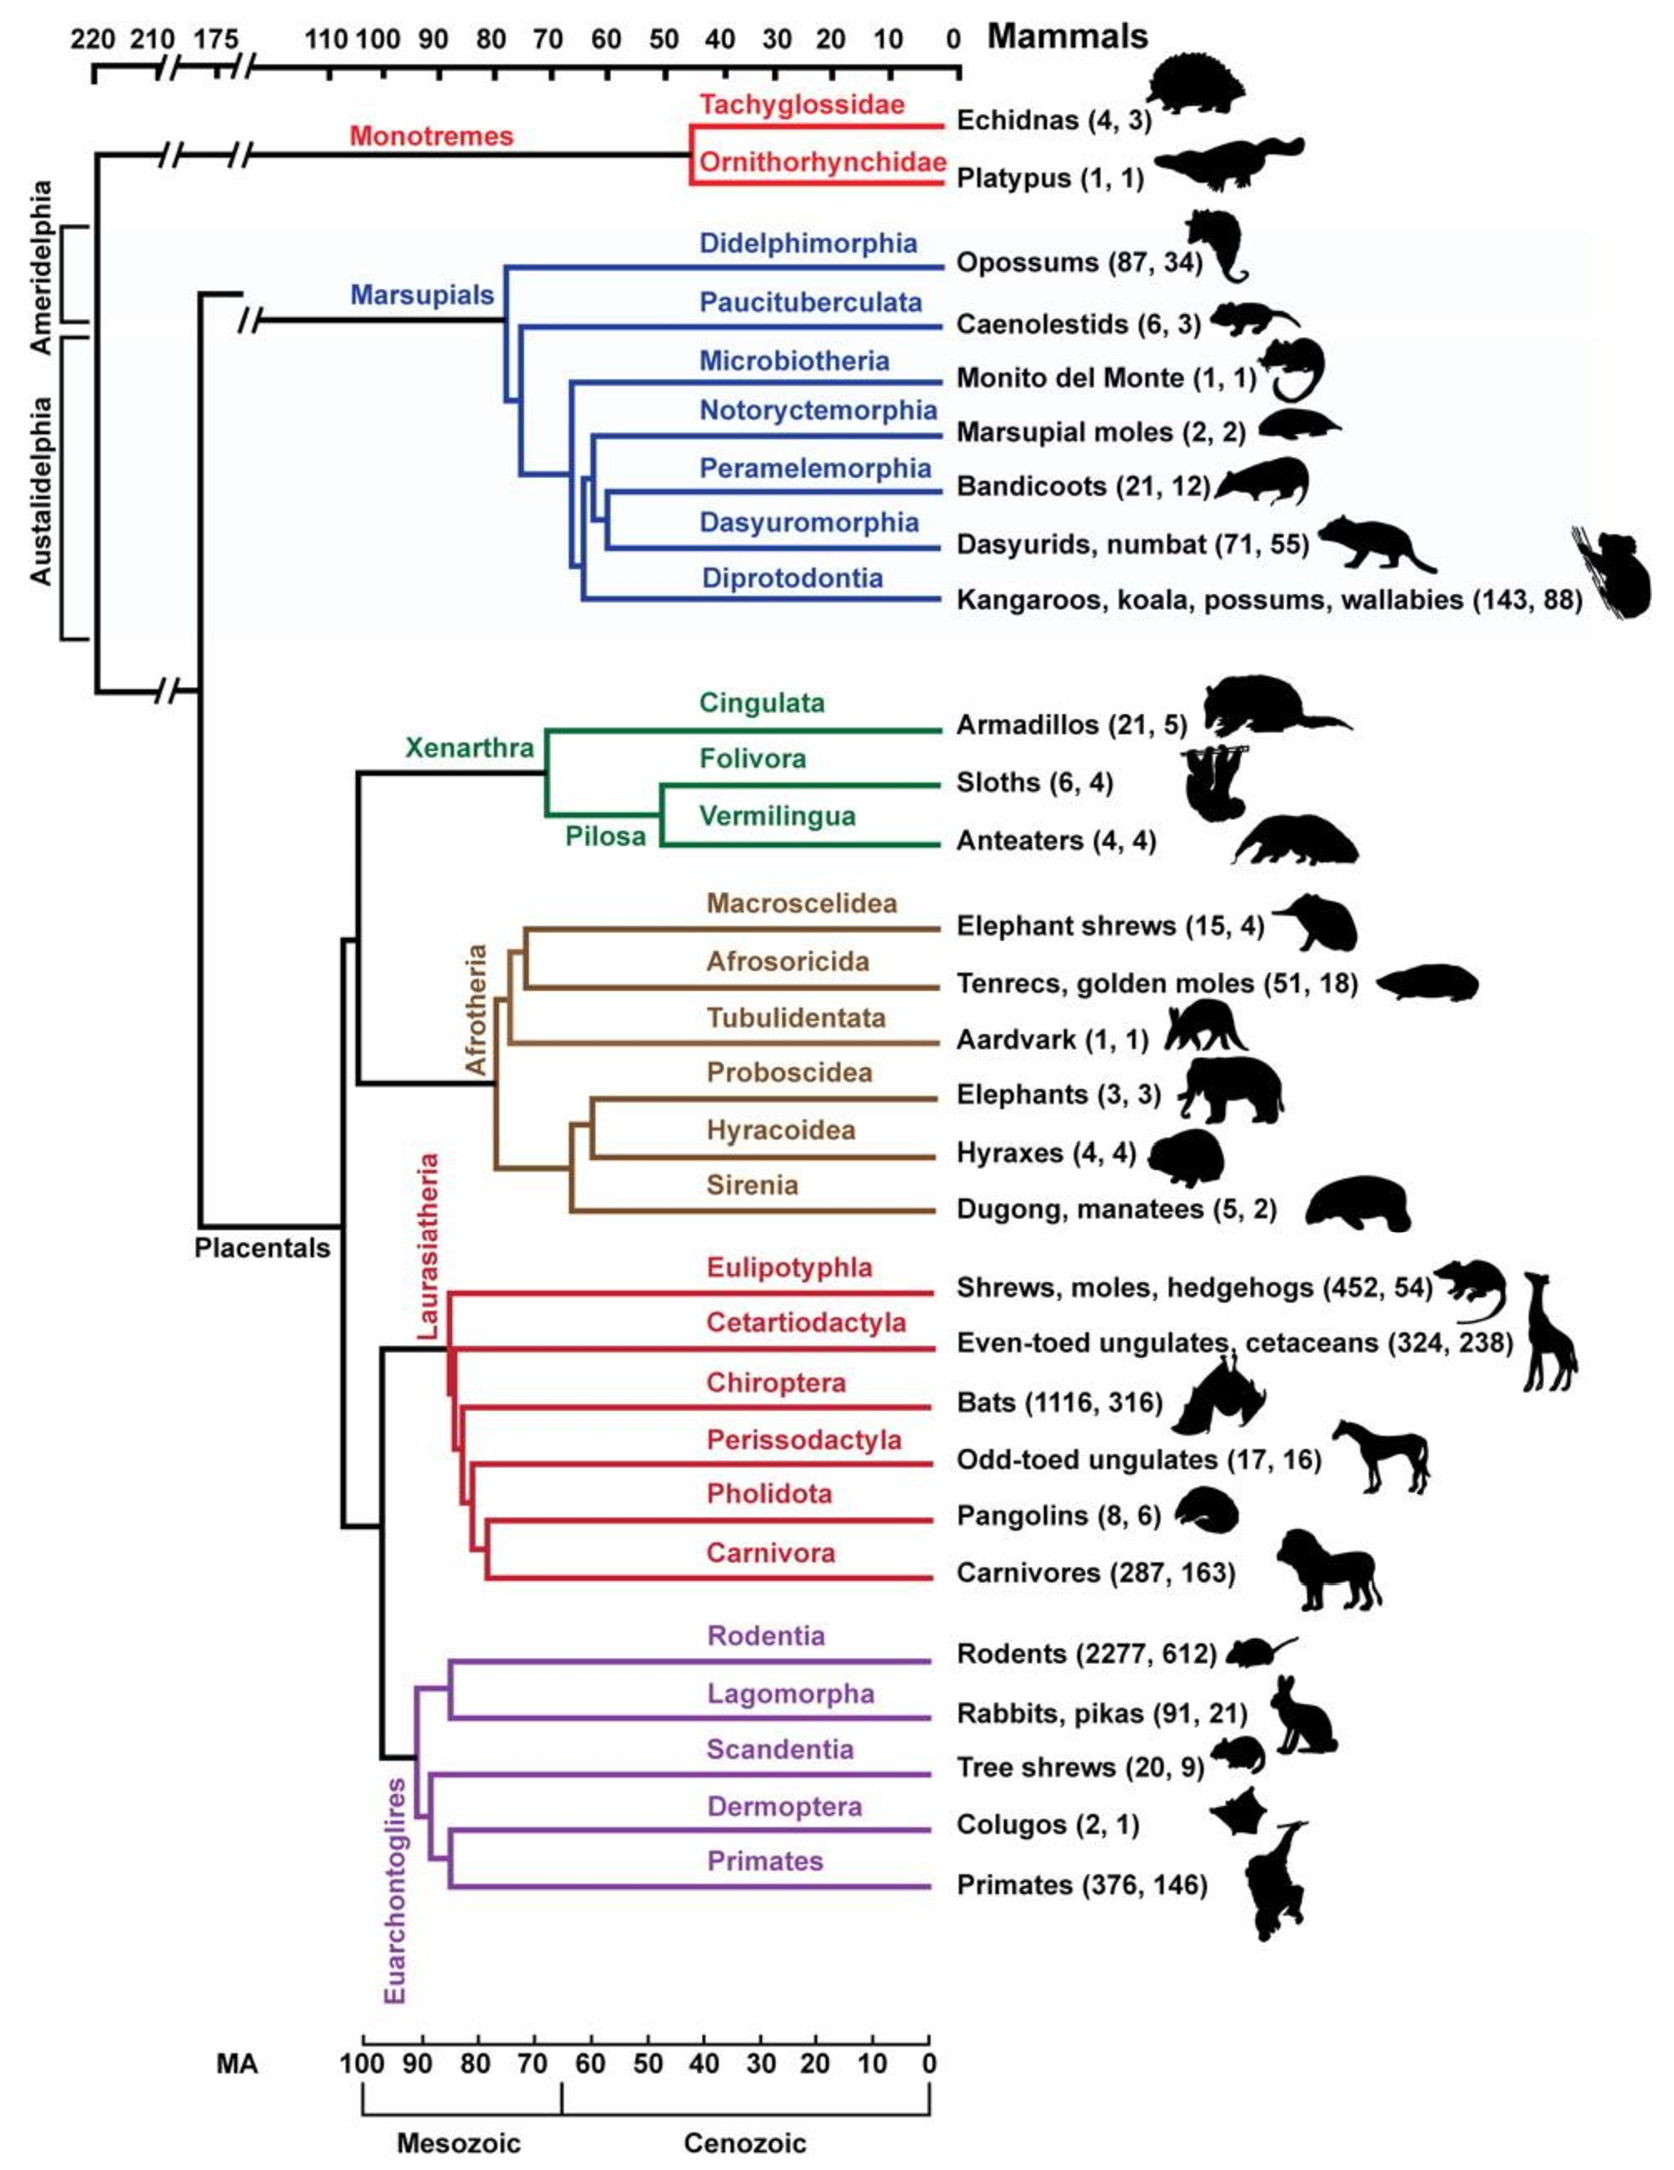
\includegraphics[scale=0.5]{Figs/mammals_10k.pdf}
\caption{A time-resolved consensus phylogeny of the major mammalian
  lineages. Topologies and dates use data from Hedges and Kumar
  \citeyearpar{Hedges2009}. Each terminal branch represents a
  mammalian family. The number of species contained in each family is
  included as the first number in parentheses after each family name
  (e.g., there are 2,227 species of rodents). Figure taken from
  \citet{Haussler2009}. }
\label{fig_mammals_10k}
\end{figure}

Before the K/T boundary, ancestral mammal and primate species were
likely smaller in size than they are today, as the ecological niches
for larger animals were occupied by dinosaurs
\citep{Martin2007,Smith2010}. Their diet is assumed to have been
largely insectivorous, as folivory in extant species is observed
mainly in larger mammals \citep{Smith2010} (but see \citet{Martin2007}
for an alternative perspective favoring a more folivorous primate
ancestor). After the K/T extinction event around 65 \ac{myr} ago,
mammals eventually diversified to occupy a wide range of the
ecological roles left vacant by extinct species, with many lineages
undergoing highly specialized morphological and behavioral adaptations
and the range of mammalian body sizes expanding by four orders of
magnitude \citep{Alroy1998}. A long-term trend towards larger body
sizes has been observed in many lineages; the hypothesis that this is
a general feature of mammalian evolution has been termed Cope's rule
\citep{Alroy1998}, though its universality is controversial
\citep{Finarelli2006,Monroe2010}.

The body size of mammals and their ancestors is an important
consideration in sequence analyses, as body size has been shown to
correlate with the overall rate of substitution in multicellular
eukaryotes
\citep{Mouse2002Initial,Hwang2004a,Welch2008,Galtier2009,Romiguier2010,
  Bromham2011}.  Other phenotypic features such as metabolic rate and
generation time have been similarly linked to genomic evolutionary
rates \citep{Martin1993,Nabholz2008}, but all three of these
characters are strongly cross-correlated in mammals, making it
difficult to isolate the effect of each particular variable on the
overall evolutionary rate or to identify the causative factor behind
such variation. Regardless, it is clear that extant mammals exhibit a
wide range of neutral evolutionary rates \citep{BinindaEmonds2007b},
with proposed explanatory factors including differences in the amount
of mutagenic free radicals associated with an animal's metabolic rate,
different rates of germ line cell divisions per year, and different
DNA repair control mechanisms \citep{Baer2007}.

\begin{figure}
\centering
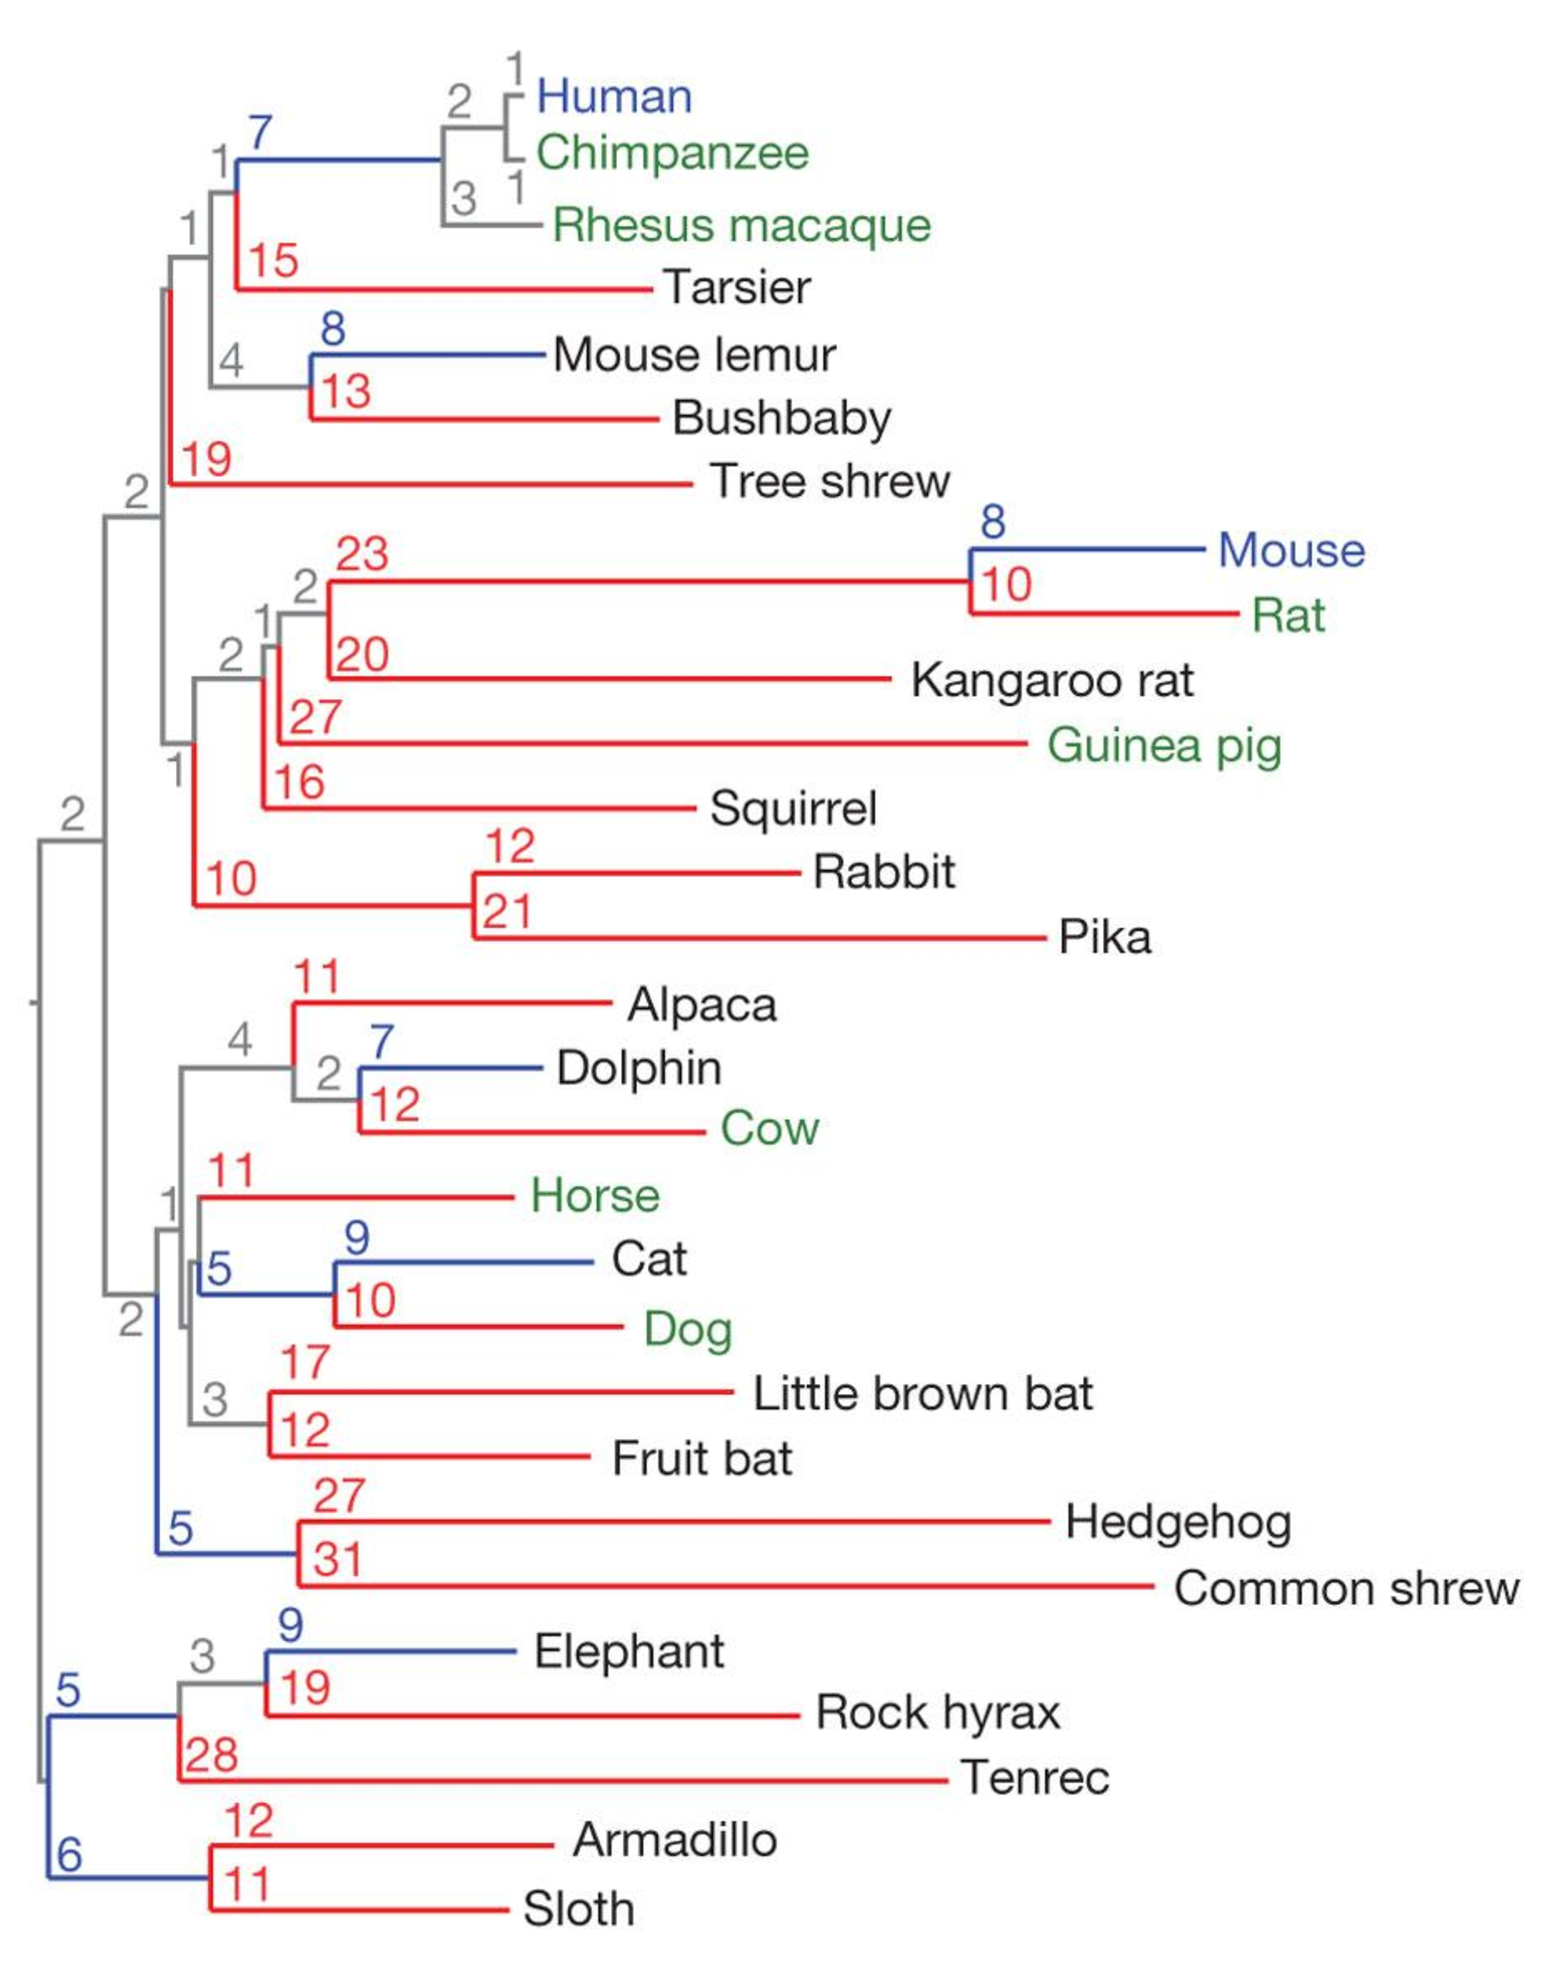
\includegraphics[scale=0.3]{Figs/mammals_29.pdf}
\caption{A phylogeny of 29 mammalian species, with branch lengths
  scaled with the neutral evolutionary rate estimated from genome-wide
  DNA alignments. Note the increased branch lengths of most rodent
  species (e.g., mouse, rat, pika) and various small members of
  Laurasiatheria (e.g., little brown bat, hedgehog, common shrew)
  relative to most primates (e.g., human, chimpanzee). Figure taken
  from \citet{LindbladToh2011}.}
\label{fig_mammals_29}
\end{figure}

The correlation between body size and neutral evolutionary rate has an
important consequence for comparative genomic studies in mammals:
extant species groups with smaller body sizes are expected to have
experienced more DNA substitutions since their common ancestor than
larger-bodied species groups, leading to increased branch lengths
within smaller-bodied clades when branches are scaled by the neutral
evolutionary rate. Figure \ref{fig_mammals_29} shows a phylogenetic
tree for 29 mammals scaled by the genome-wide rate of observed
substitutions, emphasizing the high observed substitution rates of
most rodents and low rates of most hominids and some larger-bodied
species from other mammalian orders. In comparative analyses where a
larger number of substitutions increases the power of a method to
detect a genomic feature or estimate an evolutionary rate (as is the
case for detecting conserved regulatory elements or
positively-selected genes), the larger branch lengths of
smaller-bodied species would be expected to result in improved power
and statistical accuracy. This effect will be especially important in
Chapter~\ref{ch_mammals1} where I compare \sw estimates of selection
pressures from groups of species from different mammalian orders.

A second biological characteristic showing significant variation
between mammals, the \ac{ne}, has important consequences for the study
of genomic regions subject to natural selection
\citep{Charlesworth2009}. \ac{ne} is a fundamental parameter in
population genetics, describing the size of an idealized population
that exhibits the same amount of dispersion of allele frequencies due
to genetic drift as the real population under study
\citep{Wright1931,Woolfit2009}. Many aspects of a population can
influence its \ac{ne}, including the census count, breeding patterns,
and geographical distribution of individuals \citep{Caballero1994},
and studies within mammals have consistently shown a much larger
\ac{ne} for rodents than for primates and for small versus large
mammals \citep{EyreWalker2002,Popadin2007,Halligan2010}, suggesting
that extant mammalian populations can significantly vary in this
parameter. It is beyond the scope of this thesis to provide a
comprehensive discussion of \ac{ne} and its importance within
population genetics and molecular evolution, but \citet{Woolfit2009}
and \citet{Charlesworth2009} provide focused reviews of the
subject. The main predicted impact of \ac{ne} on the study of fixed
substitutions between species is that slightly deleterious mutations
are more likely to become fixed within a population having a small
\ac{ne} versus a population with a large \ac{ne}. Closely tied to this
effect is the prediction of the nearly neutral thoery of molecular
evolution \citep{Kimura1985} that many mutations in protein-coding
regions are slightly deleterious and thus subject to this dependence
on \ac{ne} \citep{Kimura1974,Kimura1985,Ohta1992}. Several empirical
studies have supported this hypothesis, showing that a different
\ac{ne} leads to different rates of protein evolution in bacteria
\citep{Moran2008,Warnecke2011}, birds \citep{Axelsson2009} and mammals
\citep{Kosiol2008,Ellegren2009} (but see \citet{Bachtrog2008} for
potentially contradictory evidence from \emph{Drosophila}). Any
analysis of comparative evolution in mammals should thus evaluated
with respect to these well-established trends; in Chapters~
\ref{ch_mammals1} and~\ref{ch_mammals2} I consider the possible
effects of \ac{ne} on the observed patterns of positive selection
within different groups of mammals, and in Chapter~\ref{ch_gorilla} I
use genome-wide comparisons to estimate ancestral \ac{ne} in our
closest primate relatives.

Some key features of the mammalian genome itself are also worth
highlighting. Mammals contain relatively large genomes (containing
roughly 3 Gb of DNA, ranging from 2.5 to 4.5 Gb) with between 20 to 80
chromosomes \citep{Bachmann1972}. The large range in chromosome count
is likely a result of the high rate of chromosomal rearrangement in
mammals \citep{Eichler2003,Pevzner2003}. Some regions termed
``rearrangement hotspots'' show especially large amounts of
large-scale genomic shuffling within mammals, and it has been
speculated that these regions have contributed to the many
lineage-specific gene family expansions which are found in mammals
\citep{Eichler2003}. Breakpoints of mammalian chromosomal
rearrangements tend to occur near transposable elements
\citep{Zhao2009}, which are small DNA sequences capable of replicating
throughout the genome \citep{Lander2001}. Transposable elements, a
diverse class of sequence elements representing a variety of
transposition mechanisms and sequence characteristics, together
comprise roughly 45\% of DNA in the human genome and have contributed
signifciantly the ancient and ongoing evolution of mammalian genomes
\citep{Lander2001,Cordaux2009}.

In contrast to the rapid turnover of noncoding DNA and high rate of
genomic rearrangement observed in mammalian genomes, the
protein-coding gene complement appears to be less variable. Initial
estimates of roughly 30,000 protein-coding
\citep{Lander2001,Mouse2002Initial} genes in the human and mouse
genomes have been lowered based on accumulating functional and
phylogenetic evidence to roughly 21,000 genes \citep{Macaque2007}; the
most recent gene annotations from \ens \citep{Flicek2011} contain
20,599 human and 21,873 mouse ``known'' protein-coding genes. A
majority of these genes are shared between all mammals: human and
mouse share an estimated 80\% of genes in a ``one-to-one'' fashion,
meaning no apparent gene duplications or deletions occurred since the
common ancestor \citep{Mouse2002Initial}, and a wider group of mammals
including platypus show detectable orthologs (including genes with
duplications or deletions in one or more lineages) in 82\% of genes
\citep{Warren2008b}. Despite the relative consistency of the mammalian
protein-coding catalogue, features such as alternative splicing and
domain concatenations have been identified as potential contributors
to mammalian phenotypic complexity and diversity \citep{Lander2001}.

In any study of vertebrate protein-coding genes, the \ac{2r} of genome
duplication hypothesis looms large. Originally proposed by
\citet{Ohno1970}, the \ac{2r} hypothesis suggests that two
polyplidization events occurred during the early evolution of the
vertebrate common ancestor, explaining the observation that
vertebrates often have up to four homologs of invertebrate genes
\citep{Hokamp2003}. For three decades the veracity of the \ac{2r}
hypothesis was hotly debated \citep{McLysaght2002,Dehal2005}, but
analyses based on comparisons between whole-genome sequences of
several fish and basal chordates have repeatedly confirmed its
predictions \citep{Kasahara2007,Putnam2008b}. In addition to having
interesting implications for the evolution of the immune system and of
morphological diversity within vertebrates
\citep{Hughes1997,Hoffmann1999,Peer2009b}, the existence of ancient
genomic duplications can cause problems in the inference of homology
relationships between genes. Many of these aspects will be considered
in more detail in Chapter~\ref{ch_orthologs} when a set of mammalian
orthologs suitable for evolutionary analysis is identified.

\section{Models of sequence evolution}
\label{section_evolution_models}

The previous section described the major genomic and evolutionary
features of mammalian species. It is important to note that the
majority of those well-established observations were made by applying
mathematical models of sequence evolution to comparative genomics
data, which is now a standard analytical approach. This section
briefly introduces the methods and models of evolutionary analysis
which will be applied throughout the remaining chapters.

As the hereditary material of all free-living organisms, DNA
represents a record of the history of life on earth. When an
individual gives rise to offspring, special segments of DNA are
replicated and passed on to all its descendants; importantly, the
processes of DNA replication and repair are imperfect
\citep{Arnheim2009} and the resulting errors, called mutations, can be
passed on to successive generations if they occur in germline
cells. In addition to being a major source of the variation between
individuals invoked in Darwin's theory of natural selection
\citep{Darwin1859a}, mutations in DNA leave a molecular record of
evolutionary relationships and of the passage of time. The gradual
accumulation of mutations in DNA, commonly observed as differences in
DNA sequences between species at the same homologous location, can be
reasonably modeled using phylogenetic trees and Markov models of
sequence evolution \citep{Yang2006}.

The earliest observations that biological sequences tend to randomly
change over time were made from sequences of proteins, the main
molecules of cellular machinery comprised of amino acid units whose
arrangement is encoded in the DNA sequences of exons within genes. In
the early 1960s, Zuckerkandl and Pauling were analyzing the amino acid
sequences of hemoglobin genes from various species. They noted that
the number of changes between sequences from different species
corresponded well with the evolutionary distance those species based
on fossil evidence; this led them to hypothesize that evolution at a
molecular level may occur at a largely constant rate
\citep{Zuckerkandl1962,Morgan1998}. Zuckerkandl and Pauling continued
to explore the implications and applications of this ``molecular
evolutionary clock'' hypothesis, using hemoglobin and cytochrome C
sequences to estimate the date of human-gorilla divergence (at 11
million years) and to infer the protein sequences of mammalian
ancestors \citep{Zuckerkandl1965}. A wide variety of evolutionary
models have subsequently been developed to describe observed patterns
of amino acid and DNA substitutions. As this thesis is concerned
largely with the application of such methods, I will only briefly
summarize the key features of the more popular evolutionary models;
\citet{Yang2006} provides a comprehensive mathematical treatment of
the main models used in practice.

The simplest Markov model for DNA substitution, proposed by
\citet{Jukes1969a}, assumes that every nucleotide has the same rate of
changing into any other nucleotide. Although the assumption of equal
rates is a reasonable starting point for modeling a random process,
the mutation of a DNA base pair is a biochemical process (or rather, a
set of potentially many unobserved biochemical processes which all
produce the same class of observable result), making the existence of
biases towards or against certain types of mutations highly
plausible. This was quickly discovered to be the case: analysis of the
ever-increasing number of available biological DNA sequences showed
that in most datasets \emph{transitions}, defined as substitutions
between two pyrimidine nucleotides (e.g., T$\to$C or C$\to$T) or
between two purine nucleotides (e.g., A$\to$G or G$\to$A), are more
common than \emph{transversions}, defined as substitutions from a
purine to a pyrimidine or vice-versa. \citet{Kimura1980} thus proposed
a more complex model, called K80 or Kimura's two-parameter model,
which accounted for this bias. Specifically, K80 extends JC69 by
incorporating an additional parameter, $\kappa$, referred to as the
transition/transversion ratio, representing the ratio of the rate of
transition substitutions to the rate of transversion
substitutions. When $\kappa$ is greater than one, transitions occur at
a higher rate than transversions, providing a better fit to most
biological datasets \citep{Brown1982}. The $\kappa$ parameter of K80 a
prototypical example of the parametric approach to building
evolutionary models, whereby a parameter is introduced into the model
which allows for a commonly-violated assumption of the simpler model
to be relaxed. Note that the value of the parameter is not specified
in the model; rather, it must be provided or estimated from the data
on a case-by-case basis, usually by \ac{ml} estimation
\citep{Whelan2001}.

Several nucleotide models were subsequently described which relax
various assumptions of the JC69 and K80 models
\citep{Whelan2001,Yang2006}. One especially unrealistic feature of K80
is its symmetric nature (meaning that the rate of substitution from
one nucleotide to another is the same as the rate of the reverse
substitution, e.g. G$\to$C = C$\to$G). A symmetric DNA Markov chain
yields equal nucleotide frequencies when the substitution process
reaches equilibrium, meaning that any starting DNA sequence, if left
to evolve long enough under such a process, will end up with equal
nucleotide frequencies. In reality, many biological sequences contain
highly unequal nucleotide frequencies (owing to a variety of possible
selective or mutationsal biases), making it inappropriate to assume an
equal base composition \citep{Yang2006}. Thus, models such as FEL
\citep{Felsenstein1981a}, HKY \citep{Hasegawa1985} and TN93
\citep{Tamura1993} were developed to allow for various combinations of
unequal base frequencies and unequal transition/transversion
ratios. The most general reversible nucleotide model, REV, includes four
parameters describing the equilibrium nucleotide frequencies and six
rate parameters, one for each possible pair of substitutions
\citep{Tavare1986}.

In contrast to the primarily parametric DNA models, evolutionary
models for amino acids have generally been estimated empirically
\citep{Whelan2001}. The JTT \citep{Jones1992} and Dayhoff
\citep{Dayhoff1978} amino acid models, developed during the early days
of evolutionary sequence analysis, were estimated using
parsimony-based counting methods. The parsimony principle was first
used to infer phylogenetic trees and ancestral protein sequences from
each set of aligned proteins within a large database. Based on those
phylogenetic trees and ancestral sequences, the entries of the 20x20
amino acid substitution matrix were populated with counts of inferred
amino acid substitutions, and these counts were used to estimate
reversible Markov substitution models. More recently, empirical amino
acid models were estimated using \ac{ml} methods, which improved upon
a number of methodological deficiencies of the parsimony approach
\citep{Adachi1996,Whelan2001b}.

At this point it should be pointed out that a few important
assumptions are shared by all of the models already described, namely
that all sites within an alignment are (a) evolving independently of
one another, (b) evolving under the same evolutionary process and at
the same evolutionary rate, and (c) related by the same underlying
phylogenetic tree. These assumptions are clearly violated in many real
datasets, so I will briefly review the development of models which
relax them to various degrees.

Independence between sites is generally a difficult assumption to
relax for computational reasons \citep{Kosiol2006c}, but the
hypermutability of CpG dinucleotides within mammalian genomes (where
CpG denotes a C nucleotide followed by a G nucleotide, the ``p''
representing the phosphodiester bond separating nucleotides on the
same strand of a DNA molecule) has provided strong impetus to
incorporate at least a dinucleotide context into models for estimating
nucleotide substitution rates from large mammalian alignments
\citep{Blake1992,Hwang2004a,Siepel2004a}. CpG hypermutability results
from the methylation and subsequent deamination of the cytosine
nucleotide at CpG sites in most mammalian genomic DNA. Although all
cytosine nucleotides are prone to deamination (whether methylated or
not), cytosine deamination produces uracil, which is removed from DNA
strands by the enzyme uracil glycosylase, allowing for DNA repair
mechanisms to replace the original cytosine. On the other hand, the
deamination of 5-methylcytosine produces thymidine, which is not
efficiently repaired and results in frequent C$\to$T transitions
\citep{Ehrlich1982,Hwang2004a}. Context-dependent substitution models
have shown that CpG mutations are by far the dominant form of mutation
in mammalian genomes, and such models have also been essential for
studying the evolution of GC content and mammalian isochores
\citep{Duret2006,Duret2008}.

The assumption of a homogeneous evolutionary process acting across all
alignment sites is often violated in real datasets of all sequence
types \citep{Yang2006,Whelan2008}, and the development of methods
allowing for this assumption to be relaxed in the analysis of various
types of sequences has long been an area of active research. Most
studies have focused on across-site variation of a single parameter
such as the evolutionary rate
\citep{Uzzell1971,Yang1994c,Yang1996,Nielsen1998}, but more complex
types of heterogeneity, such as heterogeneity in the entire rate
matrix which describes the evolutionary process, have also been
explored \citep{Lartillot2004} . The approach generally taken for
variation of a single parameter is to describe the rate (or whichever
parameter is being modeled as varying across sites) for each site as a
random draw from a statistical distribution. In this way, the
mathematically convenient assumption of independence between sites is
upheld while sites are allowed to vary according to the parameter of
interest. The gamma distribution is commonly used for this purpose, as
it contains only one parameter if the mean rate is normalized to
1. This parameter, $\alpha$, is typically estimated from the data and
has a very clear interpretation: low values of $\alpha$ reflect a
L-shaped gamma distribution with a large amount of rate variation,
while high values of $\alpha$ reflect a bell-shaped distribution where
most sites have the average rate.

The final assumption of a single phylogenetic tree relating all sites
within a sequence has been less studied. Simulations have been used to
evaluate the potential impact of recombination
\citet{Anisimova2003,Shriner2003} and gene conversion
\citet{Casola2009} on the use of evolutionary codon models (introduced
in the next section) to detect positive selection, finding that
moderate levels of false positive occur when the assumption of a
single tree is violated. Simulations have also been used to estimate
the impact of recombination on reconstruction of ancestral sequences
\citep{Busto2010} and phylogeny inference \citep{Schierup2000}. In
virus genetics where recombination is commonly encountered, methods
have been developed to automate the identification and handling of
recombination events in evolutionary analyses \citep{Pond2006}. In
comparative genomic analyses of closely-related species, the tree
relating the species' sequences may vary across the genome due to
\ac{ils}. This is encountered in the analysis of great ape genes
presented in Chapter \ref{ch_gorilla}, where a simple filtering scheme
was used to remove sites potentially subject to \ac{ils}.

\section{Detecting purifying and positive selection in proteins}
\label{section_codon_models}

Proteins are functionally active as folded, structured amino acid
molecules, but the genes which encode them replicate and mutate as DNA
molecules. The connection between DNA and protein is mediated by the
genetic code, which describes how non-overlapping codons, or triplets
of nucleotides within the coding sequence of a protein-coding gene,
are translated by the ribosome and tRNA molecules into polymers of the
20 common amino acids. Since there are $4^3=64$ possible codons and
only 20 amino acids, the genetic code is degenerate (i.e., multiple
codons are translated into the same amino acid). This degeneracy is
concentrated in the third codon position, with many codons differing
by only their third nucleotide coding for the same amino acid, but
some degeneracy also exists in the first position. No codons differing
by their second nucleotide encode the same amino acid. Only two amino
acids, methionine and tryptophan, are encoded by just one codon, and
three codons are stop codons used to signal the end of the peptide
chain.

The degeneracy of the genetic code causes some changes on the DNA
level to be \syn, meaning they result in no change to the encoded
amino acid sequence, while others are \nsyn, meaning they result in an
altered protein sequence. The decoupled nature of the process of DNA
mutation, which is presumably ``unaware'' of the genetic code and
affects all nucleotides equally, and the process of natural selection,
which acts on phenotypes typically (but not exclusively) affected by
protein structure, suggests that a comparison of rates of \nsyn and
\syn substitution would allow the influence of natural selection
acting on a protein to be detected while inherently correcting for the
neutral mutation rate. Indeed, the potential of this approach was
noted by various researchers as soon as large-scale DNA sequencing
became practical \citep{Kimura1977,Jukes1979}, and the comparison of
the rate of \nsyn substitution ($d$N) and the rate of \syn
substitution ($d$S) has been a cornerstone of the evolutionary
analysis of proteins ever since \citep{Yang2006}. Various techniques
were historically used to estimate \dn and \ds \citep{Yang2000c}, but
most modern software is based on one of the two parametric Markov
models for coding sequence evolution independently proposed by
\citet{Goldman1994a} and \citet{Muse1994} or, when an empirical codon
model is desirable, a version of the model estimated by
\citet{Kosiol2007}.

Although the two parametric codon models differ in the details of how
nucleotide and codon frequencies are handled
\citep{Yang2000c,Bierne2003a}, they are similar in that each
incorporates a selection parameter $\omega$, representing the ratio of
\dn and \ds, into a Markov model of coding sequence evolution. The
$\omega$ parameter has a simple interpretation, namely that it
measures the ``the net effect of selection at the protein level''
\citep{Yang2000CodonSubstitution}. When $\omega=1$, natural selection
acts neither for nor against protein change, and the sequence is said
to be evolving neutrally; when $\omega<1$, selection acts to conserve
the protein sequence, exerting a so-called purifying selective
pressure; when $\omega>1$, selection acts to change the protein
sequence, exerting a so-called positive selective pressure. Within the
context of population genetics, the $\omega$ parameter can be linked
to $s$, the selective coefficient of an allele segregating in the
population \citep{Nielsen2003,Nielsen2005b,Kryazhimskiy2008}, with
$\omega>1$ corresponding to $s>0$ and $\omega<1$ corresponding to
$s<0$. This interpretation involves many assumptions, however, and has
found little practical use \citep{Nielsen2003,Nielsen2005b}.

For either of these Markov codon models, parameters (including
$\omega$, $\kappa$, and branch lengths for the model of
\citet{Goldman1994a}) can be numerically optimized for a given
alignment and phylogeny by \ac{ml} using Felsenstein's pruning
algorithm \citep{Felsenstein1981a,Goldman1994a,Yang2000c}. In their
initial description of the model, \citet{Goldman1994a} presented an
example modification to the model which allowed for heterogeneous
substitution rates across sites using an approach similar to that
described above for nucleotide models. Much subsequent work has been
focused on developing models allowing for variation of $\omega$ across
sites in the alignment
\citep{Nielsen1998,Yang2000CodonSubstitution,Yang2002,
  Wong2004,Yang2005Bayes,Massingham2005}, between branches in the tree
\citep{Yang1998a}, or both \citep{Yang2002b,Zhang2005}.  A detailed
account of these developments will not be presented here
(\citet{Anisimova2009} provide a comprehensive review of the
state-of-the-art in probabilistic codon models), but three codon-based
models in particular are used extensively throughout this thesis to
examine patterns of natural selection within mammalian proteins: the
branch model and sites models implemented in the \ac{paml} program by
Ziheng Yang \citep{Yang2007PAML} and the \ac{slr} method implemented
in the \ac{slr} program by Tim Massingham \citep{Massingham2005}. Each
of these models is introduced in more detail below.

\subsection{Branch and sites models in PAML}

For a long time, the $\omega$ ratio was almost always calculated as an
average value across an entire protein \citep{Sharp1997}. Functional
and structural constraints within a protein sequence might dominate
the gene-averaged signal of evolutionary constraint, however, even if
positive selection has acted on some portion of the protein. In some
cases, such as when the amount of computational power or data
available is limited, averaging $\omega$ across sites is a reasonable
compromise, but as computer and sequencing technologies rapidly
developed in the late 1990s, that compromise was becoming less
necessary and whole-gene estimates less justifiable. Whole-gene
$\omega$ estimates were shown to lack power \citep{Endo1996}, and
although ad-hoc analyses of $\omega$ within specific regions of proteins
were more sensitive \citep{Hughes1988}, they were limited to cases
where prior knowledge of the tertiary or domain structure of a protein
could be used to identify subsets of the protein for analysis.

As a statistically rigorous alternative, Ziheng Yang and collaborators
adopted a random sites approach to modeling variation of the $\omega$
ratio across sites for the PAML software. This implementation
typically favored modeling $\omega$ variation with a gamma or beta
distribution, discretized into a predefined number of site classes for
computational efficiency. To identify positive selection with
statistical confidence, a variety of \acp{lrt} were developed. The
\ac{lrt} is a widely-used technique which allows a specific hypothesis
to be tested by comparing the probabilistic fit, known as the
likelihood, of two nested models to a given dataset
\citep{Fisher1925}. (Two models are nested when one model is a special
case of the other, as is the case when one model is equivalent to the
other model with a parameter held at a fixed value.)  In the context
of detecting positive selection, the most effective \acp{lrt}
typically compare a model allowing for some variation of $\omega$, but
not allowing $\omega>1$, to a more complex model which allows for
$\omega>1$ (the former model being nested within the
latter). \citet{Nielsen1998} initially proposed a few simple \acp{lrt}
for detecting positive selection; these were further expanded and
evaluated by \citet{Yang2000CodonSubstitution}, and
\citet{Anisimova2001} performed extensive simulations assessing the
power and accuracy of these tests. The current release of PAML
recommends two \acp{lrt} for detecting positive selection acting at a
subset of sites within genes: \mbox{M2a--M1a} and \mbox{M8--M7} (see
Table 1 in \citet{Wong2004} for a complete description of each
model). PAML also implements a method for identifying which individual
sites show strong evidence for positive selection. This method, called
the Bayes Empirical Bayes method and described in
\citet{Yang2005Bayes}, calculates for each site an approximate
posterior probability that it has been subject to positive
selection. I evaluate the power of this method for detecting \sw
positive selection in Chapter \ref{ch_indels1}.

Codon models relaxing the assumption of a constant $\omega$ throughout
the branches of the tree, but not across sites, were also developed
and implemented in PAML \citep{Yang1998,Yang1998a}. Although these
models have received less attention and use than the branch-site
models which allow $\omega$ to vary across both sites and branches
\citep{Zhang2005}, they may be useful when branch lengths are small
and parameter estimation under the complex branch-site models is
difficult, or when variation of $\omega$ across sites is not of
interest. These models are used in Chapter \ref{ch_gorilla} to
construct a series of \acp{lrt} for detecting accelerated evolution
along specific branches of the great ape tree.

\subsection{The Sitewise Likelihood Ratio method}

In contrast to PAML's approach to site-specific evolutionary analysis,
where a \ac{lrt} for positive selection within a gene is first
performed and, subject to a significant \ac{lrt} result, \sw posterior
probabilities for positive selection are then inferred, the \ac{slr}
method \citep{Massingham2005} was specifically designed for the
sitewise estimation of purifying and positive selection. \ac{slr} is
based on an explicit Markov model of codon evolution similar to that
of \citet{Goldman1994a}. No assumptions are made regarding the
distribution of $\omega$ ratios within the alignment; instead, the
value of $\omega$ is considered to be an independent parameter at each
site. As the estimation of model parameters and calulation of
likelihood values to perform an exact \ac{lrt} at each site would
involve an expensive high-dimensional optimization, \ac{slr} uses two
approximations which greatly reduce the computational complexity:
first, common parameters are estimated under the M0 model
\citep{Yang2000CodonSubstitution} with one $\omega$ for all sites
instead of the more parameter-rich true null model, and second, the
\sw $\omega$ parameter is estimated independently at each site under
the simplifying assumption that each site's contribution to the common
parameters is minimal \citep{Massingham2005}. In practical terms,
\ac{slr} uses the common parameters and the alignment data at each
alignment site to calculate a sitewise statistic for non-neutral
evolution. This statistic is based on a likelihood-ratio test where
the null model is neutral evolution ($\omega=1$) and the alternative
model is either purifying or positive selection ($\omega<1$ or
$\omega>1$, respectively). The raw statistic measures the strength of
evidence for non-neutral evolution at each site, and the observed
statistic can be compared to its theoretical distribution under the
null model, \chisq, to identify sites with evidence for purifying or
positive selection at a desired significance threshold. Simulations
performed by \citet{Massingham2005} showed \ac{slr} to perform as well
as or better than PAML’s random sites models; Chapter \ref{ch_indels1}
provides further assessment of the power of the \ac{slr} method to
detect \sw positive selection under a wide range of conditions, and in
Chapters \ref{ch_mammals1} and \ref{ch_mammals2} I apply \ac{slr} on a
large scale to analyze genome-wide patterns of \sw positive selection
in mammals.

\section{Outline of the thesis}

This thesis describes three largely independent studies centered
around the theme of using codon models to analyze patterns of
selective constraint in mammalian genomes.

Chapter \ref{ch_indels1} describes a simulation study I conducted to
evaluate the impact of alignment error on detecting \sw positive
selection. The widespread adoption of powerful methods for sequence
analysis has been somewhat hampered by a lack of understanding of the
limitations of, and sources of error inherent within, those
methods. Without such knowledge, researchers could either avoid using
such methods for fear of producing misleading results, or blindly
apply such methods without regard for possible errors. Both paths have
been taken by others with respect to the issue of alignment error in
detecting positive selection. As a first step towards an improved
understanding of alignment error and its impact on downstream
evolutionary analyses, I performed a thorough examination of the
impact of alignment error by comparing different aligners, trees, and
methods for detecting positive selection. This work has been recently
published \citep{Jordan2011} and is presented in Chapter
\ref{ch_indels1} largely unmodified from its published form.

With whole-genome sequences quickly accruing in the databases at an
ever-increasing pace, I devoted a large part of my research effort
towards applying evolutionary codon models on a large scale to
mammalian and primate genomes. The rest of the thesis reflects this
focus, presenting two major empirical analyses. Chapters
\ref{ch_orthologs}, \ref{ch_mammals1} and \ref{ch_mammals2} describe
in three sections a genome-wide analysis of \sw selective pressures in
mammals that was performed in collaboration with the \acf{mgp}; a more
detailed description of the \acp{mgp} and my involvement in the
analysis is provided as a preface to Chapter \ref{ch_orthologs}. A
highly summarized version of the results of this analyses was recently
published \citep{LindbladToh2011}, but the version presented here
differs in that a more recent dataset was used and the methods and
results are described in considerably more detail. Particular
attention was paid to identifying (and in some cases ameliorating)
possible sources of error and to comparing the current results with
those from previous similar studies in the literature.

Chapter \ref{ch_gorilla} presents a more detailed survey of
genome-wide evolutionary patterns within a much more closely-related
group of mammals, the African great apes. This study was the result of
a collaboration with Stephen Montgomery and Nick Mundy as part of the
gorilla genome analysis group led by the Wellcome Trust Sanger
Institute, and a manuscript including the major results from our
analysis is currently under review. As a few aspects of the study
design and interpretation of results were performed by collaborators
as well as myself, those items which do not represent entirely my own
work are clearly indicated. As in the mammalian analysis, attention
was paid to assessing the potential impact of known and unknown
sources of error on the conclusions drawn. The short branches
separating the great apes meant that even small amounts of sequencing
error could yield incorrect results.

Finally, Chapter \ref{ch_conclusions} briefly ties together the
themes developed within each of the prior chapters, summarizing the
main contributions of my research towards the field and describing
planned future areas of research.

%************************************************
\chapter{The effects of alignment error and alignment filtering on the sitewise detection of positive selection}
%************************************************

\section{Introduction}

\subsection{Methods for detecting sitewise positive selection}

\subsection{Substitution and indel processes in simulating protein-coding sequence evolution}

\section{Models and parameters for simulating the evolution of mammalian genes}

\subsection{Distribution of selective pressures}

\subsection{Phylogenetic tree size and shape}

\subsection{Frequency and size distribution of insertions and deletions}

\section{Analysis of the alignment error simulation results}

\section{Methods for filtering alignments}

\section{Analysis of the alignment filtering simulation results}

%************************************************
\chapter{Curating a set of genome-wide orthologous mammalian gene alignments}
\label{ch_orthologs}
%************************************************

\section{Introduction}

\section{Low-coverage genomes in the Ensembl database}

The prevalence of missing sequence data and fragmented contigs in
low-coverage genomes presents a unique set of problems for the
generation of transcript annotations. In recognition of these
differences, the procedure used by the Ensembl database to annotate
genomes assembled from low-coverage data is distinct from the usual
gene-building pipeline \citep{TODO, Ensembl 2006}. Briefly, a
whole-genome alignment is produced between the human genome and each
low-coverage target, and gene models are projected from human to the
target genome. Small frame-disrupting insertions or deletions within
orthologous exons are corrected, and missing exons are padded with Ns
in order to obtain the correct transcript length.

The inclusion of these error-correcting features allows intact, if not
complete, coding transcripts to be generated for low-coverage
genomes. The Compara gene family pipeline uses the set of transcripts
from each species as its input \citep{TODO, Ensembl Compara}, so the
quality of the gene models from each species has a direct impact on
the overall quality and accuracy of gene trees. Although the reliance
on genome-wide alignments to, and gene annotations from, a reference
genome could be criticised for potentially causing a bias towards the
genomic properties of the reference, this approach is a reasonable
workaround in the absence of higher-coverage sequence data or a
painstakingly curated assembly. Furthermore, the gene model error-correcting
features of the Ensembl pipeline are especially beneficial, making
more complicated methods for correcting errors from low-coverage
genomes such as those described by \citep{TODO, PLoS One hubisz and
  siepel} seem largely unnecessary.


\section{The Ensembl Compara gene tree pipeline}

All genomic data and gene trees used for this analysis were sourced
from version 63 of the Ensembl Compara database \citep{TODO, Ensembl
  2010 and EnsemblCompara GeneTrees}. Although a complete description
of the design, implementation, and validation of the pipeline behind
the Ensembl database is beyond the scope of this thesis, I will
briefly outline the major aspects of the approach, focusing on a few
details which are relevant to the current sitewise analysis and the
ensuing discussion.

The Compara pipeline begins with a set of protein-coding transcripts
collected from each individual species' annotation database. This step
is not exactly straightforward, as the prevalence of alternative
splicing in Eutherian mammals makes it common for a single gene to
harbor many different transcript structures. In terms of biology and
evolution, alternative splicing is a very interesting
phenomenon. Tightly linked to the evolutionary innovation of
regulatory control and tissue-specific gene expression, the existence
of multiple transcripts per gene is one of the likely substrates of
biological and developmental complexity within vertebrates and mammals
as compared to single-celled eukaryotes, which show less developmental
complexity but largely similar numbers of genes \citep{TODO}. Further
evidence of the unique evolutionary characteristics of
alternatively-spliced exons comes from molecular evolutionary studies
which have shown such exons to show, on average, higher levels of
evolutionary constraint, possibly owing to the importance of exonic
splice enhancers in modulating the inclusion or exclusion of their
associated exons \citep{TODO}.

However, in terms of organizing biological data, pervasive alternative
splicing---with XYZ\% of human genes containing at least two (and up
to several dozen) transcripts per gene \citep{TODO}, showing tissue-specific and
species-specific expression patterns, different levels of overall
transcription, and sometimes comprising mutually exclusive exons---is
somewhat burdensome. The first problem is the fact that primary data
on alternative transcript structures (e.g., resulting from expressed
sequence tags, RNA-seq, or proteomics experiments) are largely absent
from most organisms with sequenced genomes. Even ignoring this lack of
data, the task of incorporating multiple transcripts per gene into an
evolutionary analysis is non-trivial, and leaves many unresolved
questions open to debate: should all transcripts be treated as
independent evolutionary entities, or should some form of
meta-transcript be produced, comprising all possible transcripts for a
given gene? Should expression levels and tissue-specificity be taken
into account (as both factors have been correlated with evolutionary
rate, e.g. \citep{TODO, TODO})? And what is the expected evolutionary
impact of the loss, gain, or modulation of the prevalence or
tissue-specificity of a given exon or transcript in one lineage? Even
a fairly shallow consideration of the topic quickly reveals layers of
complexity that would quickly hinder many large-scale evolutionary
analyses such as the current one, whose main goals are to understand
the levels of evolutionary constraint of some subset of genes (or
protein-coding sites) within some subset of species.

As a result of these difficulties, the current design of the Compara
pipeline only incorporates one 'canonical' transcript per gene into
the evolutionary analysis and the resulting inferred gene trees. This
reflects a conscious decision to sacrifice some biological fidelity
for reduced design complexity and computational load (as the inclusion
of multiple transcripts would inevitably require some amount of
additional processing and/or calculation). Unfortunately, this only
somewhat alleviates the problem, shifting the burden from ``how to
deal with multiple transcripts in a comparative setting'' to ``how to
choose the best representative transcript for each gene.'' In the case
of a gene with many transcripts of varying sizes containing many
non-overlapping exons, the negative consequences of choosing a
non-optimal transcript are clear: too short of a transcript could
exclude important sequence information from the dataset, while
transcripts with spurious exons (resulting from misannotation or
erroneous experimental evidence for a transcript) could introduce
potentially large amounts of non-orthologous, nonfunctional, or
nonconserved sequence into the evolutionary analysis.

Fortunately, the consensus coding sequence (CCDS) project was
initiated in 2005 to ``identify a core set of human and mouse protein
coding regions that are consistently annotated and of high quality''
\citep{TODO, Pruitt et al. 2009 Gen Res}. Although the transcripts
that satisfy these two criteria will not necessarily be the same as
those which meet the desired definition of ``the best representative
transcript for use in an evolutionary study,'' the confidence that one
can have in the quality and consistency of CCDS transcripts helps to
reduce the prevalence of potentially damaging errors in the Compara
pipeline.  Thus, in the current release (version 63), the
``representative'' transcript used for the Compara pipeline is chosen
on the basis of (a) existence within the CCDS set of transcripts and
(b) the total length of the transcript's coding sequence. The
combination of these two factors can be expected to identify a
reasonably representative transcript, at least for the human and mouse
genomes. The situation will be similar for genomes whose Ensembl
annotation is derived largely from synteny and orthology to human and
mouse annotated genes, but two classes of genomes---those resulting
from low-coverage sequencing and those from more distant species whose
annotations are derived from largely independent data sources---will
still suffer from some amount error in the form of poor transcript
choice.

Once the set of canonical transcripts is chosen, the Compara pipeline
performs an all-against-all protein BLAST search (using the Washington
University variant of BLAST) and clusters genes into groups of
evolutionarily-related sequences using \hclust, an
implementation of a hierarchical clustering algorithm for sparse
graphs. Sequences are aligned using MCoffee, a meta-aligner algorithm
which combines the results from different aligners into one alignment
using a maximum-consistency criterion. The aligners used for the
M-Coffee alignment include XXX, YYY, and ZZZ. Finally, the aligned
sequences are input to TreeBeST, which infers a gene tree (including
gene duplication and loss events) given a set of aligned sequences and
a known species tree \citep{TODO}. The type of the homology
relationship between each pair of genes (e.g., one-to-one ortholog,
one-to-many ortholog, within-species paralog) is determined using a
simple set of rules based on the structure of the inferred gene tree
and the annotation of ancestral nodes where a duplication event has
likely occurred.

The Compara pipeline has been a part of the Ensembl ecosystem at least
since its first mention in \citep{TODO}. Remarkably, aside from slight
tweaks to the protein clustering method and some changes in the exact
aligners used, the pipeline has changed little from its original
published form \citep{TODO}. In part, this lack of change reflects the
ease with which sets of vertebrate orthologs can be identified using
the existing methodology, lying in stark contrast to the equivalent
task in sets of insect or fungal genomes where divergence levels
between extant sequences are much larger \citep{TODO} and the shape of
the underlying species tree may be uncertain and/or unknown
\citep{TODO}, making the development of specialized methods or
extensive manual annotation necessary \citep{TODO}. This is equivalent
to saying that Ensembl's pipeline, while not perfect in its orthology
predictions or tree inferences (as indicated in a series of
back-and-forth papers between Ensembl scientists and XYZ,
\citep{TODO}), has proved sufficiently accurate enough that an
extensive reworking of the system has not yet been deemed
necessary. Additional validation of this approach comes in the form of
Treefam \citep{TODO}, a database of animal gene trees which applies a
similar set of tools to infer gene trees from a more diverse set of
genomes, with largely similar results.

\textcolor{red}{[Something about Ensembl being directed at inferreing
    gene tree topologies, and not being vetted for use in estimates of
    selective constraint]}

\textcolor{red}{[Introduce the structure of the next few subsections:
    ways of massaging / filtering the Ensembl data to fit with the
    needs of the current project]}

\section{Identifying orthologous subtrees within large mammalian gene families}

The first task in preparing the Ensembl data for sitewise analysis was
to identify and extract a biologically meaningful set of orthologous
mammalian subtrees from the set of gene trees within the Compara
database. This was necessary because many Compara gene trees contain
multiple sets of Eutherian orthologs linked by ancient gene
duplication events, while I wished to study the evolution of each
individual set of Eutherian orthologous genes. In other words, Compara
gene trees are over-clustered with respect to the core set of
Eutherian orthologs.

Evidence for this over-clustering comes from Table \ref{table1}, which
shows the number of root Compara gene trees which contain zero, one,
or multiple genes in human, zebrafish and drosphila, as well as Figure
\ref{fig1}, which shows the distribution of gene counts in the set of
root Compara gene trees. The percentage of Compara trees with 2 or
more human genes is strikingly high, at XYZ\%. If each Compara tree
contained one single set of Eutherian orthologs, then the proportion
of trees with multiple human gene copies could only be explained by an
unrealistically high rate of gene duplication. A more parsimonious
explanation would be that many Ensembl trees represent not one group
of Eutherian orthologs, but two or more sets of Eutherian orthologous
gene trees joined by one or more ancient duplications. This
explanation is further supported by Figure \ref{fig1}, which shows
concentrations of gene counts centered roughly around whole-integer
multiples of the number of vertebrate species present in the Ensembl
database (shown as gray dotted lines).

The prevalence of over-clustered Eutherian orthologs in the Compara
database is easily explained by a combination of the \hclust algorithm
used for the hierarchical clustering step, which uses only protein
distances as its source of clustering information, and the wide range
of protein evolutionary rates in the vertebrate genome. As I mentioned
in the previous subsection, the Compara pipeline uses all-by-all
protein BLAST E-value scores and the \hclust algorithm to produce sets
of sequences containing minimal average within-group E-values. No
additional biological information, such as the source species of each
sequence or the overall taxonomic coverage of each cluster, is used in
identifying clusters, and no attempt is made to fit clusters to an
expected model of orthologous gene evolution. On the one hand, the
lack of additional information and assumptions allows the algorithm to
remain simple and the clustering behavior to remain consistent across
different groups of genomes; on the other hand, a number of technical
(in the sense of non-biologically meaningful) parameters and
thresholds must be tuned in order to result in the desired cluster
sizes and contents. Importantly, even after these parameters are tuned
to perform well on the dataset as a whole, the reliance on protein
distances alone means that fast-evolving proteins will be more likely
to be under-clustered and slow-evolving proteins will be more likely
to be over-clustered. Given that the protein evolutionary rate varies
widely within a genome (\TODO{in a study of vertebrate genes, XYZ et
al. found $K_a$ values ranging from ZZZ to YYY}), the excess of
over-clustered orthologs in the Compara database is understandable and
even somewhat expected.

I should note that my use of the phrase ``over-clustered'' refers only
to over-clustering with respect to the current goal of analyzing
independent sets of orthologous genes within Eutherian
mammals. Certainly these large ``over-clustered'' trees, which
represent a more distant evolutionary history than a single Eutherian
orthologous group, are just as accurate with respect to the true
evolutionary history of the genes as more narrow groupings would
be. Furthermore, the inclusion of a deeper evolutionary context may
sometimes be more useful to users of the Compara database, for whom an
understanding of the overall evolutionary history of a gene may be the
topic of primary interest.

\begin{figure}[h]
\centering
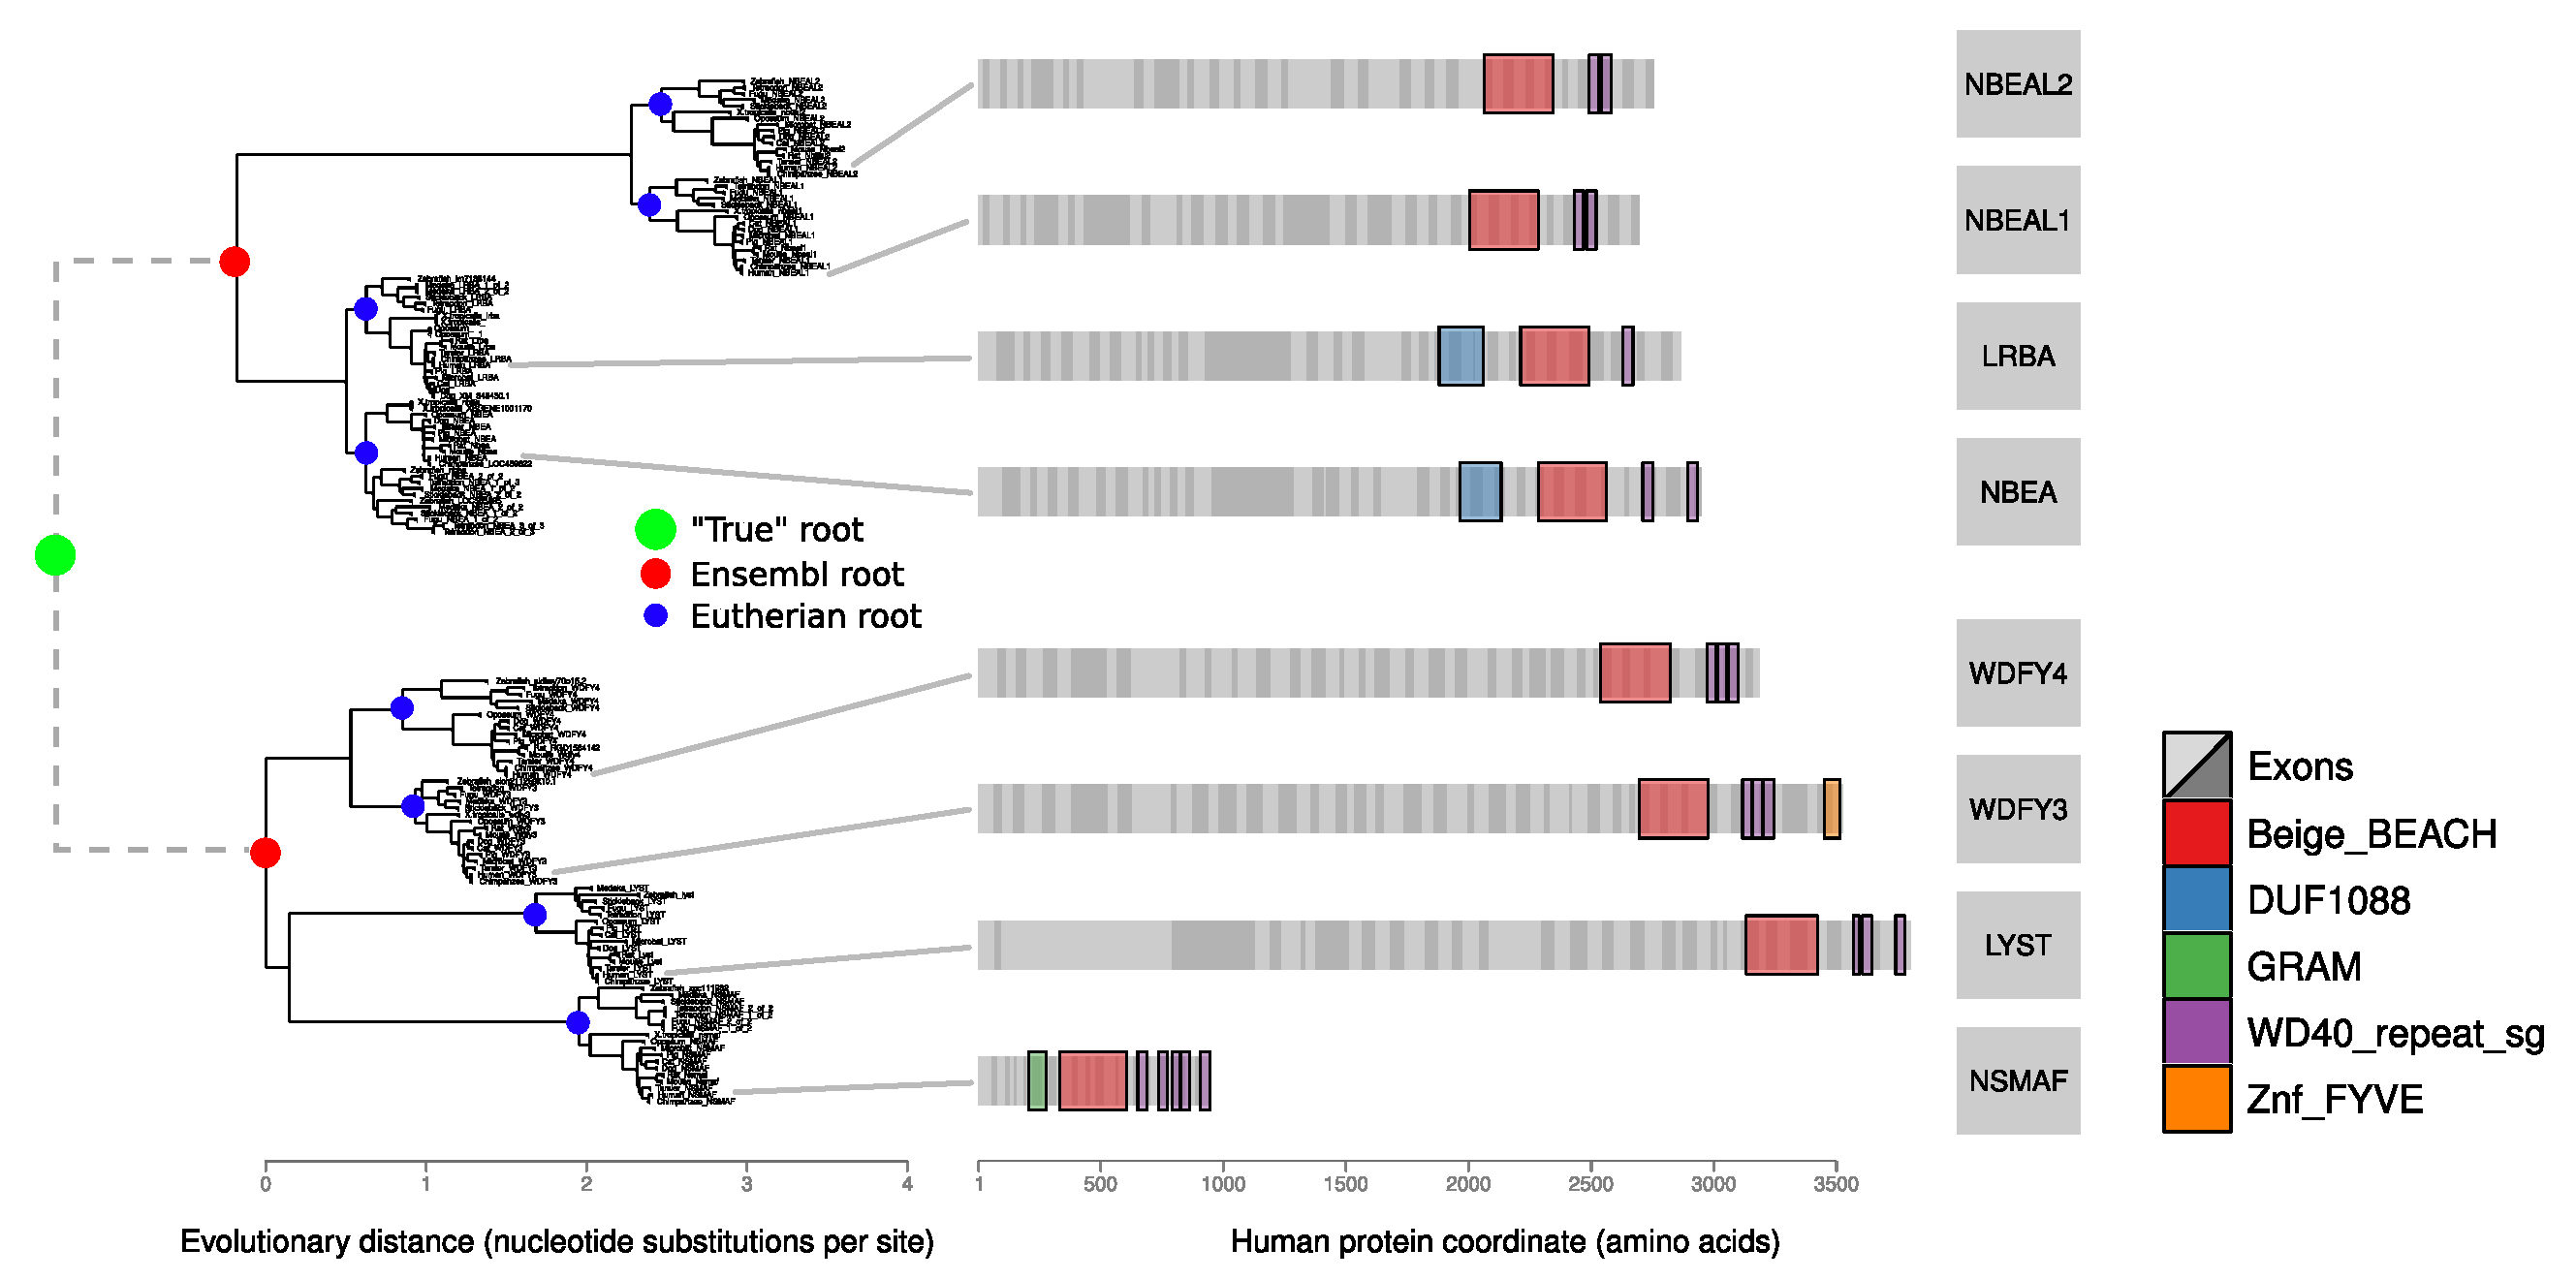
\includegraphics[scale=0.3]{Figs/nbeal2_full.pdf}
\caption{The evolutionary history of the human \gene{neurobeachin-like 2}
  gene (\gene{NBEAL2}) and its paralogs. Left, two phylogenetic trees from
  Ensembl Compara (release 60) are shown, summarizing the evolution of
  \gene{NBEAL2} and its three paralogs (top) and \gene{LYST}, a presumed distant
  paralog of \gene{NBEAL2}, and its three paralogs (bottom) in 15
  vertebrate species. The phylogeny shows that \gene{NBEAL2} is
  taxonomically conserved and distinct from its paralogs. Red dots
  highlight the root nodes of Ensembl gene trees, blue dots highlight
  the root nodes of Eutherian orthologous subtrees, and a dashed line
  with a green dot represents the putative paralogous relationship
  (with a hypothetical root) between the two Ensembl gene
  trees. Right, the exon and domain structure of each human gene is
  shown: exons are displayed alternating shades of gray, and Pfam
  domain annotations are colored according to their Pfam identifier.}
\label{nbeal2}
\end{figure}

Take for example the gene \gene{NBEAL2} and its human paralogs, whose gene
trees, exon structures and domain classifications were extracted from
Ensembl v62 and summarized in Figure \ref{nbeal2}. A recent medical
sequencing project identified \gene{NBEAL2}, a gene of previously unknown
function, as the putative causative gene for gray platelet syndrome, a
predominantly recessive platelet disorder resulting in moderate to
severe bleeding \citep{TODO}. It was important for the
authors of this study to ensure that the \gene{NBEAL2} gene is well-conserved
across mammals and distinct from its paralogs. The Compara pipeline
clustered \gene{NBEAL2} with three of its closest paralogs into one tree (and
similarly clustered four more distant \gene{NBEAL2} paralogs into a separate
tree), yielding two views which together showed both the full
taxonomic coverage of the \gene{NBEAL2} \subtr{} and the large amount of
separation between paralogs. Had each Eutherian ortholog been
displayed independently in Ensembl (using the blue ``Eutherian root'' nodes in
Figure \ref{nbeal2}), it would have been more difficult to make such
claims regarding the evolutionary history of \gene{NBEAL2} without further
analysis. Conversely, had the Compara pipeline been even more
inclusive in its clustering step and identified a hypothetical deeper
root connecting these two sets of trees (represented by the green node
in Figure \ref{nbeal2}), the connection between these eight genes
would have been more immediately apparent.

For the purposes of the current mammalian sitewise analysis, however,
it was important to isolate individual mammalian gene trees for
further processing and sitewise analysis. To this end, I designed a
simple scheme for splitting gene trees into non-overlapping subtrees
based on flexible taxonomic coverage criteria.

I hypothesized that a relatively simple set of rules based on
taxonomic coverage would be sufficient to identify most largely
orthologous mammalian subtrees. This hypothesis was based on two
well-established observations in mammalian genomes. First, the
existence of two rounds of whole-genome duplication preceding the
evolution of vertebrates \citep{TODO} suggested that many of the
ancient duplication events contained within Ensembl gene trees
occurred before the divergence of \mmls, making it possible to cleanly
separate out taxonomically complete \mmln \subtr{}s in the majority of
cases. This would not be possible if duplication events were common
and spread evenly throughout the \mmln tree; if that were the case,
many duplication events would have occurred after the divergence of
some or all of the major \mmln groups, resulting in a larger
proportion of \mmln genes with ``internal'' duplications and, thus,
fewer singly orthologous trees with high taxonomic coverage. Second,
the overall low rate of gene duplication and loss in mammals
\citep{TODO, mammalian gene trees PLoS One} (excluding, of course, the
aforementioned whole-genome duplication events) predicts that few
mammalian gene trees will be subject to one or more gene duplication
or loss events. In other words, most mammalian gene trees should
contain sequences from a majority of mammalian species, so the
effectiveness of using taxonomic coverage to identify mammalian
\subtr{}s should be largely unaffected by individual (i.e., post-2R)
gene duplication or loss events. The potential utility of taxonomic
coverage was further bolstered by the star-like shape of the mammalian
tree: star-like trees contain more branch length within terminal
lineages than ladder-like trees with an equivalent total branch
length, making it less likely that a gene duplication or loss event
(if such events occurred randomly throughout the mammalian tree) would
result in a significant disruption to the taxonomic coverage of the
gene tree.

The taxonomic-based tree splitting scheme works as follows. For every
internal node $N$ of each Compara gene tree, the taxonomic coverage
(TC) was calculated for several vertebrate clades. The TC for node $N$
and clade $C$ is given by $TC(N,C) = species(N) / species(C) $, where
$species(N)$ is the number of unique species represented by the
sequences beneath node $N$ and $species(C)$ is the number of species
within the vertebrate clade $C$. The tree is traversed from root to
tip, and if a given set of TC constraints (referred to as the subtree
constraints) are satisfied by both \subtr{}s below node $i$, then the
tree is split into two \subtr{}s at node $i$ (with the new trees
having root nodes placed at the two child nodes, $i_a$ and $i_b$). The
traversal continues recursively until every node is tested. If only
the original root node satisfies the subtree constraints, then the
entire Compara tree is included in the resulting tree set; if the
entire Compara tree fails to satisfy the subtree constraints, it is
excluded altogether.

I chose a variety of subtree constraints based on the structure of the
vertebrate phylogeny, all of which were run against the 18,613 gene
trees within the Compara database to generate several genome-wide sets
of subtrees. Table \ref{subtree_constraints} shows the details of the
various subtree constraints I used; the clade names (e.g.,
$TC(Primates)$) are used to refer to sets of species contained within
the Ensembl database, as defined by the NCBI taxonomy. The NCBI
taxonomy of species contained in Ensembl is shown in Figure
\ref{ncbi_tree}.

For the Ingroup and Outgroup categories of subtree constraints, a TC
value of greater than 0.6 was required for a single taxonomic
clade. If the required TC value for a clade were set to 1, then all
subtrees containing deletions in any species within the clade of
interest would be rejected. On the other hand, requiring a TC value of
less than 0.5 would allow for a truly singly-orthologous tree to be
split into two \subtr{}s, with one tree having a TC below 0.5, and the
other tree (containing the other half of the species) also having a TC
below 0.5. Thus, 0.6 seemed to be a reasonable TC requirement for
isolating \subtr{}s with reasonable taxonomic coverage while allowing
for some amount of gene deletion.

Two additional types of constraints were designed for use in the
MammalSubgroups and MammalSubgroupsPlusOutgoup methods. Inspired by
the alignment filtering method from Pollard et al. \citeyearpar{TODO},
which required sequence data from all three major mammalian clades
(Primates, Glires, and Laurasiatheria) to be present for a column to
pass through the filter, the $TC_{all}$ constraint requires that the
TC for all of the included clades is above a given threshold. To
complement the $TC_{all}$ constraint, the $TC_{any}$ constraint
requires that the TC for any of the included clades is above a given
threshold. These more complicated methods were included in the
analysis in case the simpler TC constraints within the Ingroup and
Outgroup categories did not perform satisfactorily.

The methods within the Orthologs category of subtree constraints were
implemented separately from the rest. Instead of splitting Compara
trees based on taxonomic criteria, the subtrees in the Orthologs
category were defined from the sets of genes annotated by Ensembl as
orthologs to each gene from a given source species. Thus, for each
gene from the source species, the Compara \subtr{} containing all of
the Ensembl-annoated orthologs was extracted and stored; this was
guaranteed to yield exactly one \subtr{} for every gene in the source
species. I chose to include human, mouse, zebrafish, and drosophila
were chosen as source species for testing. This approach differs from
the tree-splitting strategy in two ways: first, it makes use of the
orthology annotations resulting from Ensembl's orthology pipeline, and
second, it does not guarantee that each \subtr{} contains a completely
unique set of genes. For example, a gene which was recently duplicated
in humans would yield two \subtr{}s, one for each human paralog, with
identical sets of non-human genes in each tree. Although the
orthology-based method might be useful when an evolutionary study is
focused on a specific target or reference species, as is often done
with human and mouse due to their finished genome sequence and
high-quality annotation, I considered it to be less applicable to the
current study due to the potential for introducing reference
genome-specific biases, such as over-representation of genes with gene
family expansions in the reference species or non-representation of
genes which have been deleted in the reference species. Still, I
expected that the sets of \subtr{}s resulting from the Ensembl
ortholog annotations would serve as a useful reference with which to
compare the other TC-based methods.

\begin{figure}
\centering
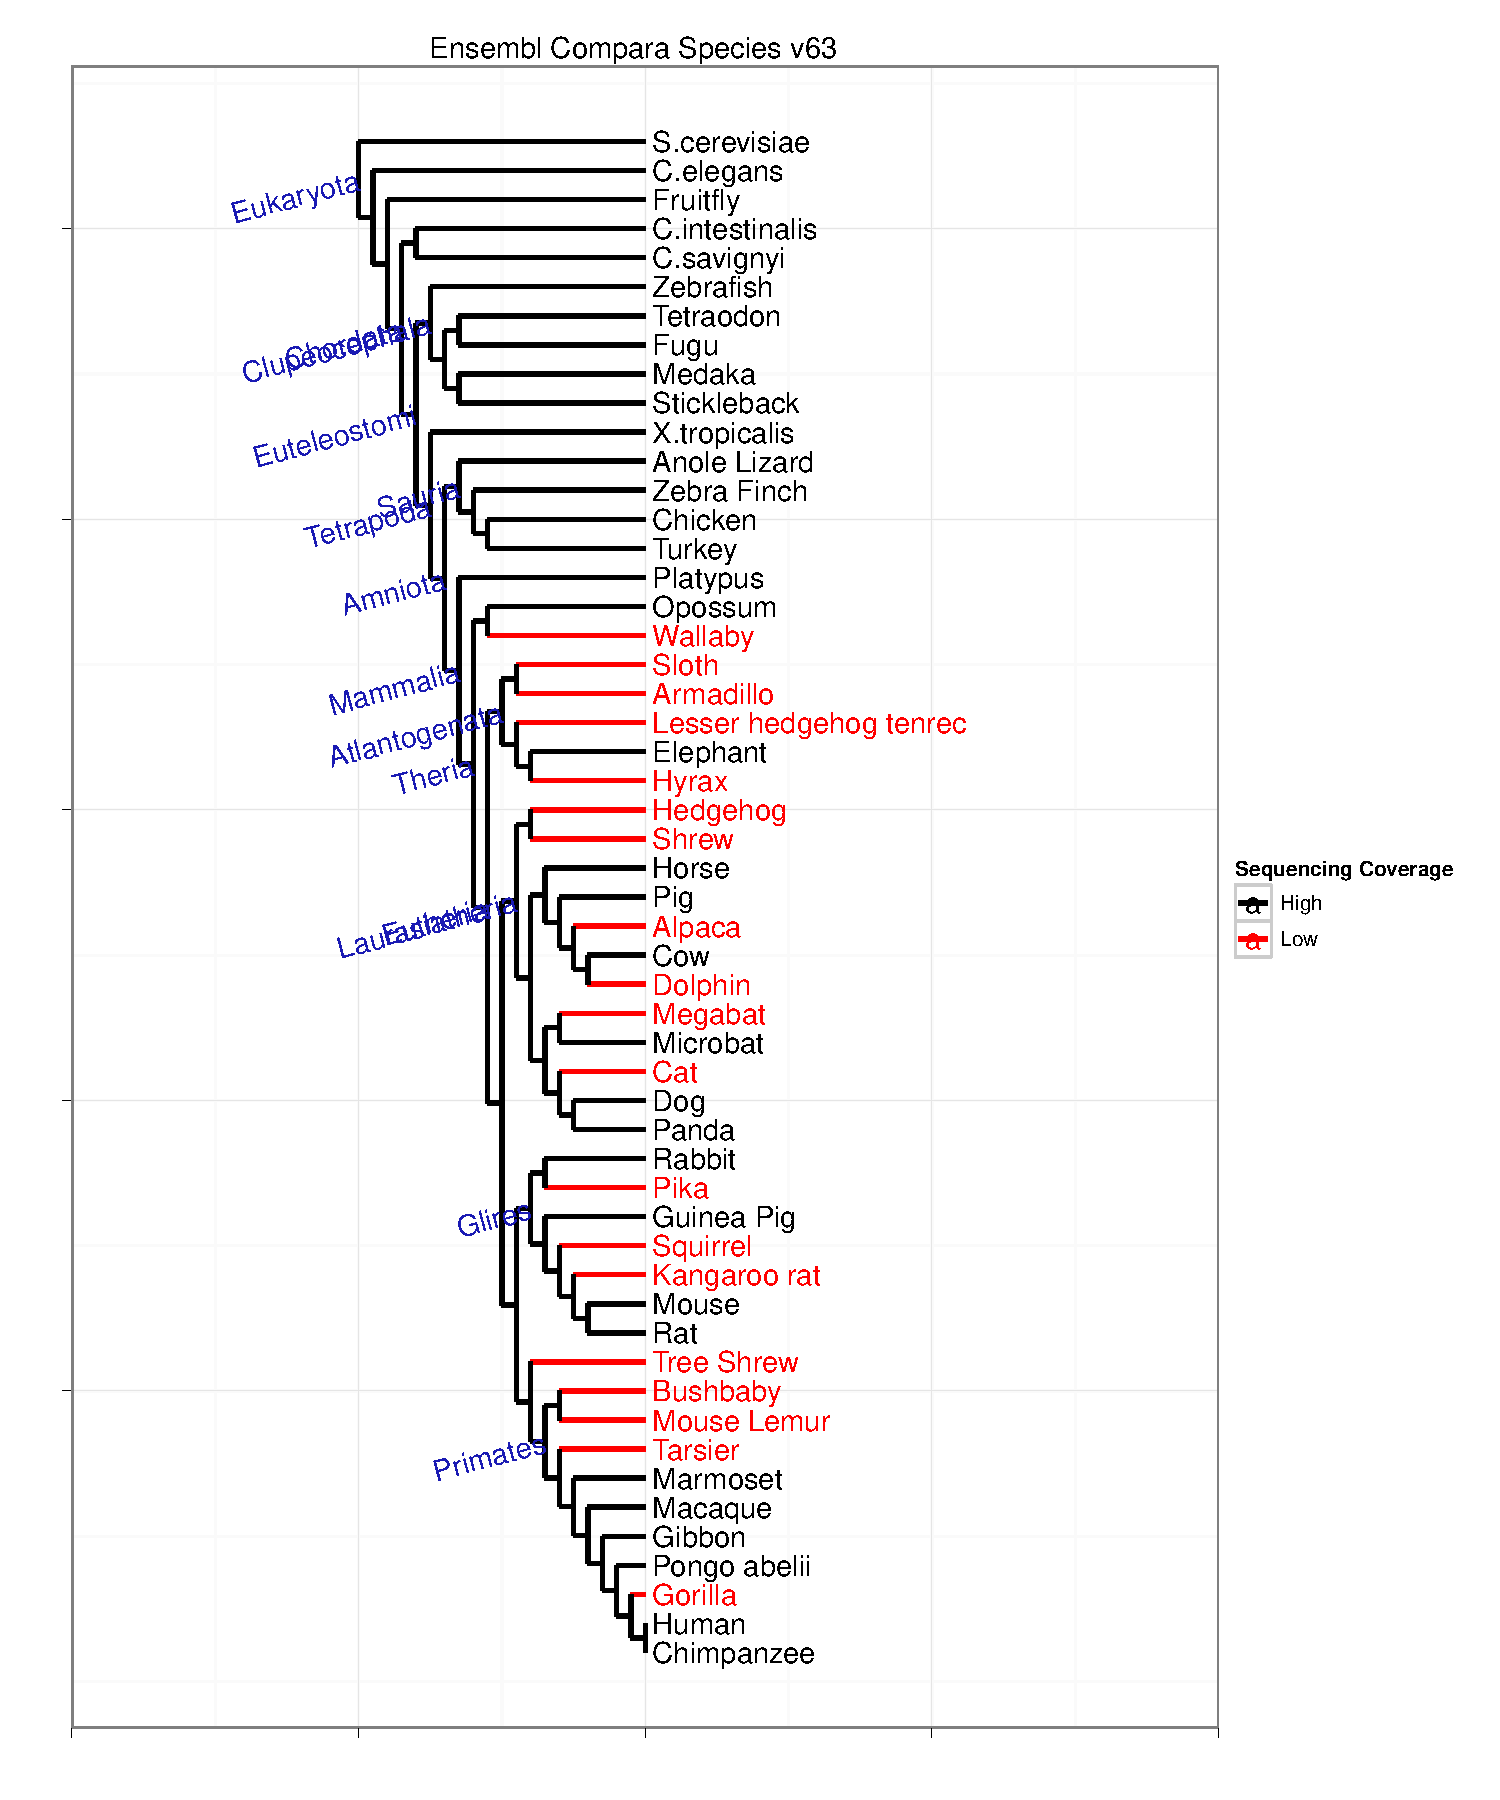
\includegraphics[scale=0.4]{Figs/compara_63_tree.pdf}
\caption{The NCBI taxonomy of species within the Ensembl Compara
  database. Note that branch lengths are not drawn to
  scale. Low-coverage genomes are labeled in red, high-coverage
  genomes are in black. Selected internal nodes, used are labeled in
  blue.}
\label{ncbi_tree}
\end{figure}


\begin{table} \footnotesize
\centering
\begin{tabular}{@{}lll@{}} \toprule
\multicolumn{2}{c}{Method} \\ \cmidrule(r){1-2}
   Category & Name & Constraints \\ \midrule
Ingroup & Primates & $TC(Primates) > 0.6$ \\
 &   Glires &  $TC(Glires) > 0.6$ \\
 &   Laurasiatheria & $TC(Laurasiatheria) > 0.6$ \\
 &   Sauria & $TC(Sauria) > 0.6$ \\
 &   Fish & $TC(Clupeocephala) > 0.6$ \\
Outgroup &  Eutheria & $TC(Eutheria) > 0.6$ \\
 &   Amniotes & $TC(Amniota) > 0.6$\\
 &   Vertebrates & $TC(Vertebrata) > 0.6$\\
 &   Fungi/Metazoa & $TC(Fungi/Metazoa) > 0.6$\\
Subgroups &  MammalSubgroups & $TC_{all}(Laur., Glires, Primates) > 0.1$\\
 &   \scriptsize{MammalSubgroupsPlusOutgroup} & $TC_{all}(Laur., Glires, Primates) > 0.1$ AND \\
 &    & $TC_{any}(Sauria, Clupeo., Ciona, Marsup.) > 0)$ \\
Orthologs & Human Orthologs & \\
 &   Mouse Orthologs &  \\
 &   Zebrafish Orthologs &  \\
 &   Drosophila Orthologs &  \\
Root Nodes & Ensembl Roots &  \\
\bottomrule
\end{tabular}
\caption{Subtree constraints used for identifying Eutherian
  orthologous subtrees. Ensembl gene trees were split into subtrees
  based on taxonomic coverage (TC) requirements at internal
  nodes. Laur. - Laurasiatheria; Clupeo. - Clupeocephala; Marsup. -
  Marsupiala}
\label{subtree_constraints}
\end{table}

\section{Analysis of genome-wide sets of orthologous mammalian trees}

The \subtr splitting schemes described in the previous subsection were
applied to the 18,607 root gene trees from the Ensembl database. In
this and the next section I will describe the resulting sets of trees
and \subtr{}s, discuss what they reveal about the evolutionary history
of vertebrates and the feasibility of using taxonomic coverage to
isolate orthologous trees for sitewise analysis, and finally, explain
my reasoning for deciding to use the subtrees based on the Eutherian
taxonomic coverage for the subsequent sitewise analysis.

\subsection{The set of root Compara gene trees}

Table \ref{ensembl_root_table} presents a summary of the set of root
Compara gene trees and the subsets of trees with more or fewer than 15
sequences.

\begin{table} \footnotesize
\centering
\begin{tabular}{lrb{2cm}rrrrrrr}
\toprule
Tree & &  Med. Size &  & \multicolumn{3}{c}{Human Content} & Human & Med. & Med. \\ \cmidrule(r){5-7}
Set & Count  & (Min / Max) & N50 & 0 & 1 & 2+ & Total & MPL & Species \\ 
  \midrule
\input{Tables/ortholog_roots_summary.txt}
   \bottomrule
\end{tabular}
\caption{Summary of the set of Ensembl Compara root trees. The 'Human
  Content' columns represent the fraction of trees which contain the
  indicated number of human genes, and 'Human Total' is the total
  number of human genes contained within the tree set. 'Med. Species'
  is the median species count across all trees. Med. - median, MPL -
  mean path length }
\label{ensembl_root_table}
\end{table}

It is somewhat surprising that nearly half of all Compara gene trees
contain few sequences: 9,378 out of 18,607 root trees constitute fewer
than 15 sequences. Given the protein-based clustering performed by the
Compara pipeline, one might expect many of these small trees to
represent portions of larger fast-evolving gene trees whose high
sequence divergences made the BLAST search step inaccurate or caused
clustering via the \hclust algorithm to be ineffective. Alternatively,
these small clusters might have resulted from exceptional
lineage-specific gene duplications or pseudogenes mis-annotated as
genes, creating tight clusters of very closely-related transcripts
that were identified by \hclust as independent gene trees. Some
evidence for the latter scenario comes from the median species counts
and mean path lengths of the smaller versus larger trees. The subset
of small root trees has a median species count of 2 compared to 47 for
the large subset, indicating that the smaller trees encompass
sequences from a very small taxonomic range. Furthermore, the median
MPL for small trees is 0.04 compared to 1.04 for the large subset,
revealing a much smaller level of sequence divergence within each
tree. Together, these summary statistics indicate that the smallest
trees in the Compara database consist of highly species-specific,
closely-related proteins that are likely artifactual gene
annotations.

Despite the existence of many small trees in the Compara database,
they comprise only a small fraction of all protein-coding
sequences. Only 4\% of the human gene set---which we expect to be
well-annotated and to contain few false positive genes due to the high
level of manual curation and the large amount of continued
scrutiny---is contained within the subset of small trees. This
indicates that whatever process is causing the Compara pipeline to
yield such a high number of small gene trees has not had too much of
an impact on the placement of the most confident set of protein-coding
genes within the database of root gene trees.

\begin{figure}
\centering
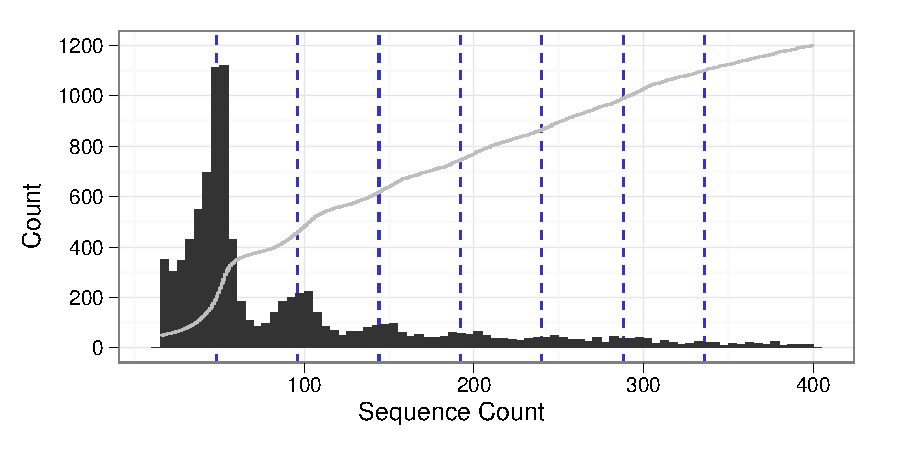
\includegraphics[scale=0.9]{Figs/ensembl_roots_hist.pdf}
\caption{Sequence counts for the set of root Compara trees. Black bars
  show a histogram of sequence counts in bins of width 5, and the gray
  line shows the cumulative fraction of sequences contained within
  trees of that size or smaller. For clarity, 9,378 trees with 15 or
  fewer sequences are not shown. Dashed blue lines are drawn at
  integral multiples of 48, the number of vertebrate species within
  Ensembl.}
\label{ensembl_roots_hist}
\end{figure}

A closer examination of the distribution of tree sizes in the set of
root Compara trees presents a clear view of the over-clustering of
mammalian orthologous trees. The black bars in Figure
\ref{ensembl_roots_hist} show the distribution of sequence counts for
all trees with more than 15 sequences, with vertical dashed lines
overlaid at multiples of 48 (the number of vertebrate species in
Ensembl release 63). The highest peak
of the histogram is at or slightly above 48 sequences, with the tree
counts quickly diminishing at larger sizes. Weaker, but still
discernable, peaks appear at larger tree sizes, with the location of
these echo-like peaks corresponding closely to the second, third and
fourth multiples of 48. The pattern of recurring peaks becomes
indistinguishable at sizes above 200, but there is still a long tail
of large trees extending out to a maximum size of 400
sequences. Overall, the distribution of tree sizes provides good
support for the situation described above, with the Compara pipeline
often clustering together two or more largely-orthologous gene trees
sharing ancient homology.

It is also interesting to characterize the set of Ensembl trees by the
proportion of all sequences which are covered by trees of a given size
or smaller. This value is plotted in Figure \ref{ensembl_roots_hist}
as a gray line. First, one can see that trees with fewer than 15
sequences (which were excluded from the plot but inlcuded in the
calculation of the cumulative fraction of sequences) represent a
trifling fraction of the sequences within Compara; this is similar,
but not identical, to the above-mentioned calculation that 4\% of
human genes are contained within these smaller trees. Second, the
steady slope of the cumulative curve contrasts with the declining
height of the histogram. This results from the increasing number of
sequences encompassed by each of the larger trees: although there are
relatively few trees with more than 300 sequences, together they
contain around 10\% of all protein-coding genes in Ensembl. Two points
along this cumulative plot are of particular interest. First, one can
identify the fraction of vertebrate proteins which exist as
identifiable paralogs. Looking at the value along the x-axis where the
largest bump in the histogram ends, at around 75 sequences, one can
see that in total around 30\% of proteins are covered by trees of 75
sequences or fewer. Since the pattern of bumps in the histogram
correlate well with the number of Ensembl vertebrate species, it would
be reasonable to state that 70\% of vertebrate proteins are contained
within large gene trees containing sequence-based evidence of ancient
paralogy. Second, a look-up in the reverse direction can identify the
tree size at which 50\% of sequences are clustered. This value
represents the size of tree that an ``average'' protein might be
clustered in, and in some ways is a more accurate characterization of
the set of gene trees than the median tree size. A similar calculation
is often performed to characterize the size distribution of contigs
(contiguous sequence blocks) within a genome assembly. This statistic,
referred to as the N50 length, is the contig length for which 50\% of
bases are contained in contigs of that size or larger
\citep{TODO}. For the Ensembl root trees, the N50 tree size is 139,
slightly less than three times the number of vertebrate species. The
N50 tree size is shown for the root trees in Table
\ref{ensembl_roots_hist} and in the table for taxonomically-defined
tree sets below.

Another way to characterize the distribution of gene trees is across
the taxonomic space. A question of particular interest to the
identification and analysis of mammalian orthologs is whether levels
of gene presence and absence are consistent across different species
and different levels of assembly quality. To investigate this question
in the context of the root Ensembl trees, data were collected by
counting the number of sequences from each species contained within
each gene tree. Results were tabulated for each species and are
presented in Figure \ref{ortholog_root_dups}, showing the number of
trees containing 0, 1, 2, or more than 3 genes from each of the 53
species in Ensembl. Comparing the range of values in the panels for
each copy count (labeled 0, 1, 2 and 3+), one finds that most trees
(8,000-11,000 within vertebrates) contain zero copies from a given
species, fewer trees contain one copy (4,000-6,000) and several
thousand contain two, three or more copies (ca. 1,000-1,500 for 2
copies and 1,500-2,000 for 3+). The plethora of trees with zero copies
from a given species is again a result of the existance of many small,
species-specific trees within the root Ensembl set. Similarly, the
high number of trees with many copies from each species reflects the
clustering of multiple orthologous sub-trees together.

A comparison of values across the range of species in Figure
\ref{ortholog_root_dups} reveals that the zero-copy count tends to
increase along with evolutionary distance from human, while the 1, 2
and 3+ copy counts tend to decrease as the distance from human
increases. Both trends are most striking at the distant end of the
tree where the five non-vertebrate species begin. For the increase in
zero-copy trees and the decrease in single-copy trees, the strength of
the trend at the highest level of divergence can be partly explained
by the very long branch lengths connecting those species to each other
and to the more well-represented vertebrate clade: the distance-based
clustering algorithm might reasonably be expected to produce more
false negatives in longer branches for a number of reasons including
the behavior of the \hclust algorithm, inaccurate BLAST E-values at
larger distances, and heterogeneity in evolutionary rates across
lineages \citep{TODO}. However, the dearth of 2 and 3+ copy counts in
non-vertebrates is most likely a signal resulting from the 2R event at
the basal vertebrate lineage, with the non-vertebrate species strongly
depleted of multi-copy duplicates compared to their vertebrate
relatives.

It is slightly concerning that human and its close primate relatives
contain fewer zero-copy genes and more one-copy and two-copy genes
than any other group of vertebrates in the set of Ensembl trees. There
is no \emph{ab initio} biological reason to expect this to be the
case, and I suspect that the existence of such a pattern, which is
fairly small in effect, is due to the widespread reliance on human
annotation and protein experimental data in the annotation of
non-human genomes. There is one region where this trend does not
appear to be the case: in the 3+ copy count for the fish species,
which is instead a result of gene duplicates retained after the third
round of genome duplication which occurred in the teleost ancestor
\citep{TODO}. The signal resulting from the teleost genome duplication
event is clearer in the sets of taxonomically-defined \subtr{}s, so I
will defer its discussion to the next subsection where those sets of trees are described.

Finally, the differences in copy counts between species with low- and
high-coverage genome sequences show the tendency of low-coverage
genome sequences to yield false negatives in the gene annotation, as
low-coverage species contain more zero-copy, roughly the same number
of one-copy, and noticeably fewer multi-copy genes than high-coverage
species. These clear effects of low sequencing coverage show that gene
absence in low-coverage genomes should not be taken as evidence for
actual gene loss and that gene duplications are systematically
underrepresented in low-coverage genomes. The former point was
emphasized in a recent critical analysis of the effect of low-coverage
genomes on gene duplication inference \citep{TODO, Milinkovitch et
  al. 2010}, but the latter point was largely ignored. Again, this
signal is also stronger in the more stringent set of \mmln orthologous
\subtr{}s and will be revisited in the next subsection.

The preceding analysis of the set of root Ensembl trees, in which I
characterised the distribution of trees with respect to size
(i.e. sequence count) and across the taxonomic space, showed that
despite the over-representation of small, species-specific trees, most
sequences are contained in trees with biologically plausible sizes
given the history of vertebrate genome duplications. The tree-based
equivalent of the N50 statistic was developed for summarizing the
distribution of differently-sized trees, and two main views of this
distribution were introduced (in Figures \ref{ortholog_root_dups} and
\ref{ensembl_roots_hist}), providing evidence for the clustering of
paralogous mammalian sub-trees and for species-based and genome
coverage-based trends in the breakdown of gene copy counts within
these trees.

\begin{landscape}
\begin{figure}
\centering
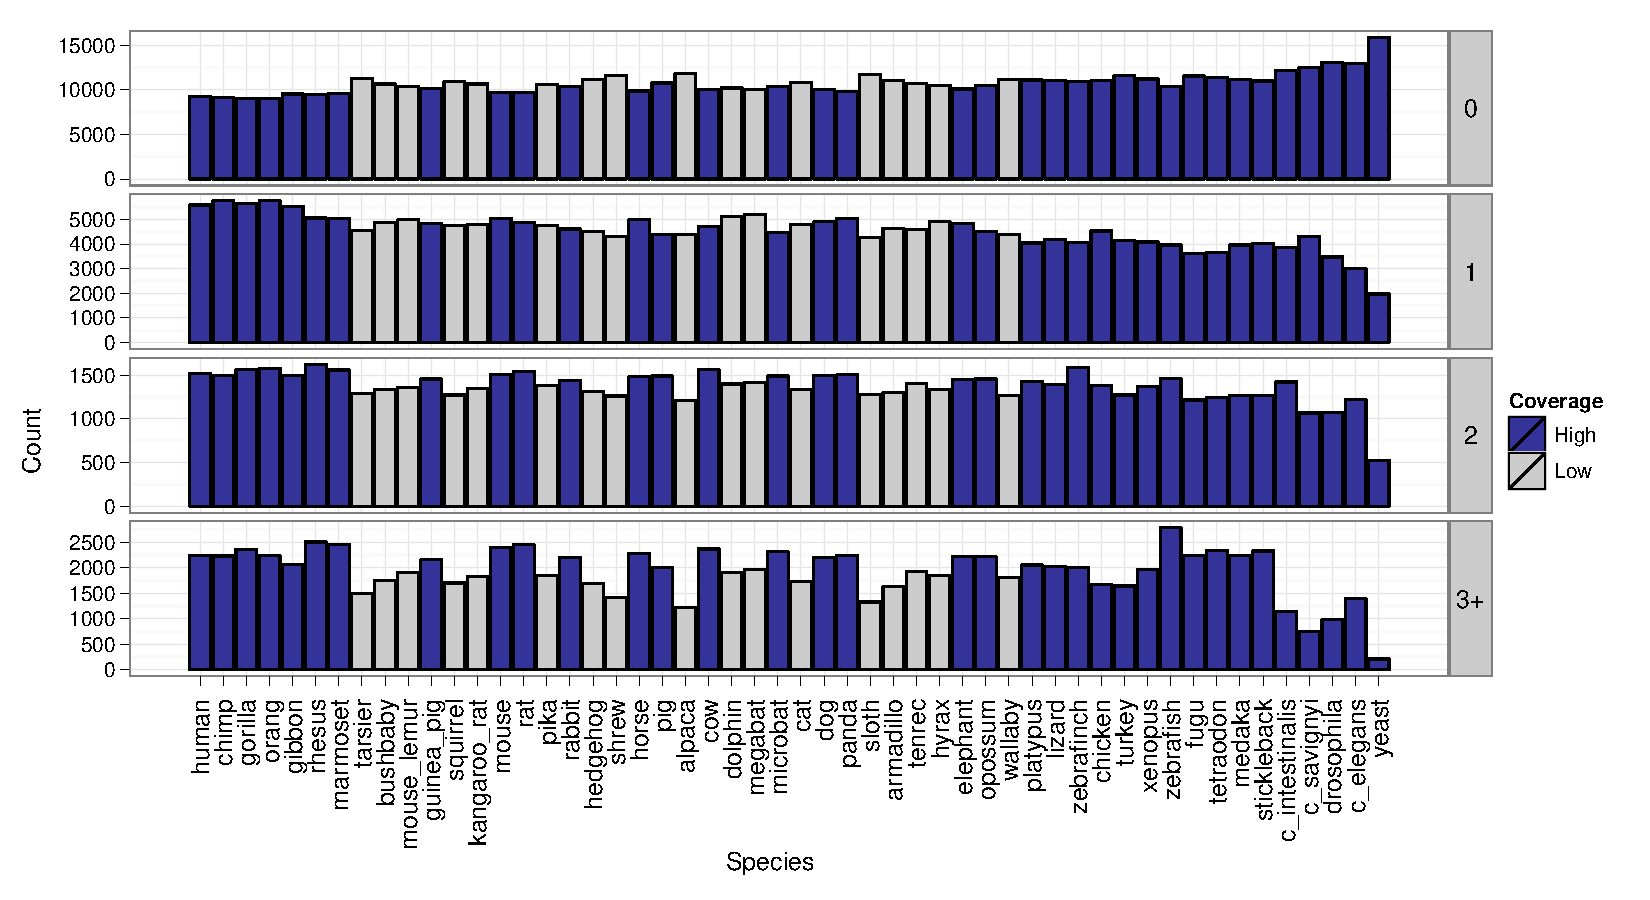
\includegraphics[scale=0.9]{Figs/ortholog_root_dups.pdf}
\caption{Taxonomic distribution of gene copy counts for the root
  Ensembl trees. The number of trees containing 0, 1, 2 or more than 3
  sequences from each species is shown. Bars are colored blue and gray
  for species with high- and low-coverage genomes, respectively. Note
  that the y-axis scale is not the same for each panel.}
\label{ortholog_root_dups}
\end{figure}
\end{landscape}

\subsection{Sets of \subtr{}s defined by taxonomic coverage and orthology annotation}

The sets of trees resulting from applying the various \subtr
extraction methods to the root Ensembl gene trees are summarised in
Table \ref{ensembl_subtree_table}, with the original Ensembl trees
included at the bottom for comparison.

The Ensembl Roots and Drosophila Orthologs sets are two clear
outliers, with much higher N50 values than any other set (139 and 125
vs. the next highest value of 56) and more trees with multiple human
copies (0.20 and 0.43 vs. the next highest value of 0.14). In fact,
the major differences between these sets are all attributable to the
excess of small species-limited trees in the Ensembl Roots group: the
Drosophila Orthologs set contains fewer trees than the Ensembl Roots
(9,210 vs. 18,607) and a larger average tree size (60 vs. 15), closely
resembling the set of Ensembl Roots with small trees removed as
summarised in the third row of Table \ref{ensembl_root_table}.

Within the Ingroup category of methods, the methods based on
mammalian TC values (Primates, Glires and Laurasiatheria) produced
largely similar sets of trees, with the Primate set containing around
2,000 more trees and covering around 1,000 more human genes than the
other two sets. A reason for the higher number and human coverage of
Primate trees is not immediately apparent, although it may
speculatively be due to an excess of primate-specific gene trees that
are not captured by non-primate TC-based criteria. Further
investigation of the trees unique to this set might reveal the root
cause of this slight discrepancy.

The Sauria and Fish tree sets stood in strong contrast to the
mammal-based methods from the Ingroup category. The Sauria clade is
represented by only four Ensembl species and diverged from the
mammalian ancestor at an early point in the evolution of amniotes. The
moderately lower number of trees (13,046 vs. 15,764 for
Laurasiatheria) and the increased proportion of trees containing
multiple human genes (0.14 vs. 0.09 for Laurasiatheria) are presumably
consequences of the lower clade size, which could affect the TC
calculation, and the long branch separating Sauria from the other
vertebrate clades. The fish-based subtree constraint produced a
strikingly different set of trees resulting from the impact of the
teleost-specific whole genome duplication on the structure of fish
gene trees. Although the Fish tree set contains a N50 value of 49
which is no different from the N50 of the other Ingroup sets, Table
\ref{ensembl_subtree_table} highlights three major differences in the
Fish set: it contains many more trees, a higher proportion of trees
with zero human copies, and a lower total human gene count than the
other Ingroup sets.

The reason for the drastically different Fish tree set is that the
tree splitting procedure identifies largest non-overlapping \subtr{}s
that satisfy the given TC criteria. Genes that were duplicated in the
teleost lineage and retained in duplicate form (as opposed to one or
both copies being lost in either of the descendant duplicate
chromosomes) would result in a gene tree with two teleost-specific
\subtr{}s, each containing a high TC value for the Clupeocephala
clade. In this case, the splitting procedure would result in two small
Fish subtrees, ``missing'' the single subtree of mammalain orthologs
because two non-overlapping trees already exceeded the TC threshold of
0.6. If, however, one of the duplicate gene copies were lost, then the
tree would resemble a typical singly-orthologous vertebrate gene tree,
and the splitting procedure would select a \subtr encompassing the
entire vertebrate clade. It follows that the presence of small,
teleost-specific gene trees in the Fish set is a signal of retained
duplicate copies, and the size distribution of trees from the Fish
set, shown in Figure \ref{ensembl_fish_hist}, shows that several
thousand trees fit the expected model. If we assume that all trees
from the Fish subset which contain zero human copies, span 5 or fewer
species, and contain 40 or fewer sequences are likely retained
duplicate genes, a total of 6,980 retained duplicates are identified,
yielding a retention rate of 17.5\%, which is very much in line with a
previously published estimate of 15\% based on a comparison of
tetraodon, fugu and zebrafish genes \citep{TODO, Brunet et al. MBE
  2006}.

\begin{figure}
\centering
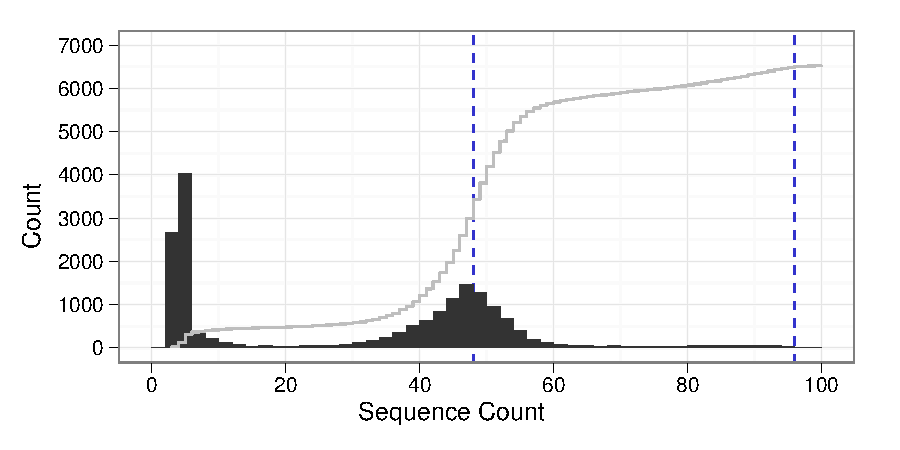
\includegraphics[scale=0.9]{Figs/ensembl_fish_hist.pdf}
\caption{Sequence counts for the set of \subtr{}s identified using the
  Fish clade taxonomic coverage constraint. Black bars show a
  histogram of sequence counts in bins of width 2, a gray line shows
  the cumulative fraction of sequences contained within trees of that
  size or smaller, and dashed blue lines are drawn at integral
  multiples of 48, the number of vertebrate species within
  Ensembl. The 255 trees with more than 100 sequences are not shown.}
\label{ensembl_roots_hist}
\end{figure}


The sets of \subtr{}s resulting from the Outgroup methods were of
special interest, as the clades used to define these TC constraints
contained all or nearly all of the mammalian species whose orthologous
genes I wished to study. The resulting sets of \subtr{}s show little
variation, owing perhaps to the large sizes of the clades and their
similar composition. Each set contained between 15 to 17 thousand
trees, N50 values of around 49, and greater than 90\% of trees
containing exactly one human sequence. These measures provided good
evidence that the tree-splitting method was effectively isolating
singly orthologous mammalian trees.  Some slight trends were apparent,
however, with the tree count decreasing, the proportion of trees with
human duplications increasing, and the overall human gene coverage
decreasing as the clade size used for the TC calculation
increased. These trends could understandably be the result of the
minimum required tree size increasing along with the clade size,
ranging from 21 for Eutheria to 32 for Fungi/Metazoa.

The Subgroups methods did not appear to produce \subtr{}s of any
higher quality or more biological interest than the Outgroup
methods. The MammalsSubgroups set was more numerous than the Outgoups
sets, but the N50 was slightly lower (46 vs. 49) and the proportion of
zero-humany trees was higher (0.18 vs. 0.01), suggesting that the
additional trees were spurious results containing fragmented species
coverage. The addition of an outgroup requirement to the
MammalSubgroupsPlusOutgroup method produced a tree set more closely
resembling the Outgroup methods, but the human gene coverage was
lower than that for any Outgroup method despite the overall higher
tree count.

Finally, the ortholog annotation-derived \subtr{}s provided for an
interesting comparison between three different ortholog sources and
between the overlapping and non-overlapping sets of \subtr{}s. As I
mentioned at the beginning of this section, the \species{Drosophila}
ortholog set was highly contrasted with the vertebrate sets due to the
two rounds of whole genome duplication. There was minimal variation
among the other ortholog sets, although it is interesting to note that
Ensembl contained 21,873 mouse protein-coding genes while human
contained only 19,991. Zebrafish, on the other hand, contained 24,540
genes, in line with the 17.5\% rate of duplicate gene retension I
estimated earlier. Overall, 76\% and 81\% of mouse and zebrafish genes
have an apparent one-to-one ortholog in human, which is slightly lower
than the 92\% of Eutheria \subtr{}s containing one human sequence.

\begin{landscape}
% latex table generated in R 2.13.0 by xtable 1.5-6 package
% Thu Sep 15 11:19:59 2011
\begin{table}
\centering
\begin{tabular}{llrb{2.5cm}rrrrrrr}
\toprule
\multicolumn{2}{c}{Method} & &  Med. Size &  & \multicolumn{3}{c}{Human Content} & Human & Med. & Med. \\ \cmidrule(r){6-8} \cmidrule(r){1-2}
Category & Name & Count  & (Min / Max) & N50 & 0 & 1 & 2+ & Total & MPL & Species \\ 
  \midrule
\input{Tables/ortholog_summary.txt}
\bottomrule
\end{tabular}
\caption{Summary of Ensembl \subtr{}s identified using taxonomic
  criteria or Ensembl ortholog annotations. The set of Ensembl root
  trees (``Ensembl Roots'') from Table \ref{ensembl_root_table} is
  included for comparison. Cells in numeric columns are shaded
  according to their value relative to other rows, with low values in
  white and high values in blue. The 'Human Content' columns represent
  the fraction of trees which contain the indicated number of human
  genes. 'Med. Species' is the median species count across all
  trees. Med. -- median, MPL -- mean path length}
\label{ensembl_subtree_table}
\end{table}
\end{landscape}

Figure \ref{ortholog_stacked_bar} shows the taxonomic distribution of
gene copy counts for the trees resulting from each of the \subtr
methods tested. By way of reference, the values shown in the separate
panels of Figure \ref{ortholog_root_dups} appear in Figure
\ref{ortholog_stacked_bar} as different-colored bars in the bottom
panel. Although the various characteristics of each of the \subtr
methods have already been discussed at length, the taxonomic view
reveals some salient features of the patterns of gene deletion and
duplication within the tree sets and shows the pervasive impact of
genome-wide duplications on the evolution of vertebrate genes. The
large fraction of species with multiple copies in Drosophila Orthologs
\subtr{}s is a result of the two rounds of vertebrate genome
evolution, while the elevated fraction of multi-copy fish trees in the
Outgroup \subtr{}s shows the impact of the teleost-specific
duplication event.

Furthermore, the relative prevalence of zero-copy and multi-copy trees
can provide some indication of whether gene deletion or gene
duplication is a more common process in vertebrate genomes. Focusing
on the four Outgroup \subtr methods, the observation of a greater
number of multi-copy trees than zero-copy genes, valid across all four
\subtr methods and throughout all mammalian species except platypus,
can be interpreted as tentative evidence for a greater number of gene
duplications than gene deletions in the evolution of mammalian
genomes. This pattern does not hold for vertebrates more distantly
related to human, however: vertebrates beyond opossum show a distinct
and consistent increase in zero-copy trees, and birds appear to
exhibit a slight clade-specific drop in the proportion of multi-copy
trees. Of course, both of these trends could be methodological
artifacts related to the \hclust algorithm or to the methods used to
assemble and annotate more distantly-related genomes.

The distributions in Figure \ref{ortholog_stacked_bar} also reveal the
pig to harbor a very high number of apparent gene deletions, unmatched
by other mammalian species and nearing the proportion of zero-copy
trees seen in platypus and more distant vertebrates. Given the
consistently low proportion of zero-copy trees for other
closely-related species, I would expect this number to change once a
finished-quality pig genome sequence is included in the Ensembl
pipeline \ref{TODO, Archivald et al. 2010}.

\begin{figure}
\centering
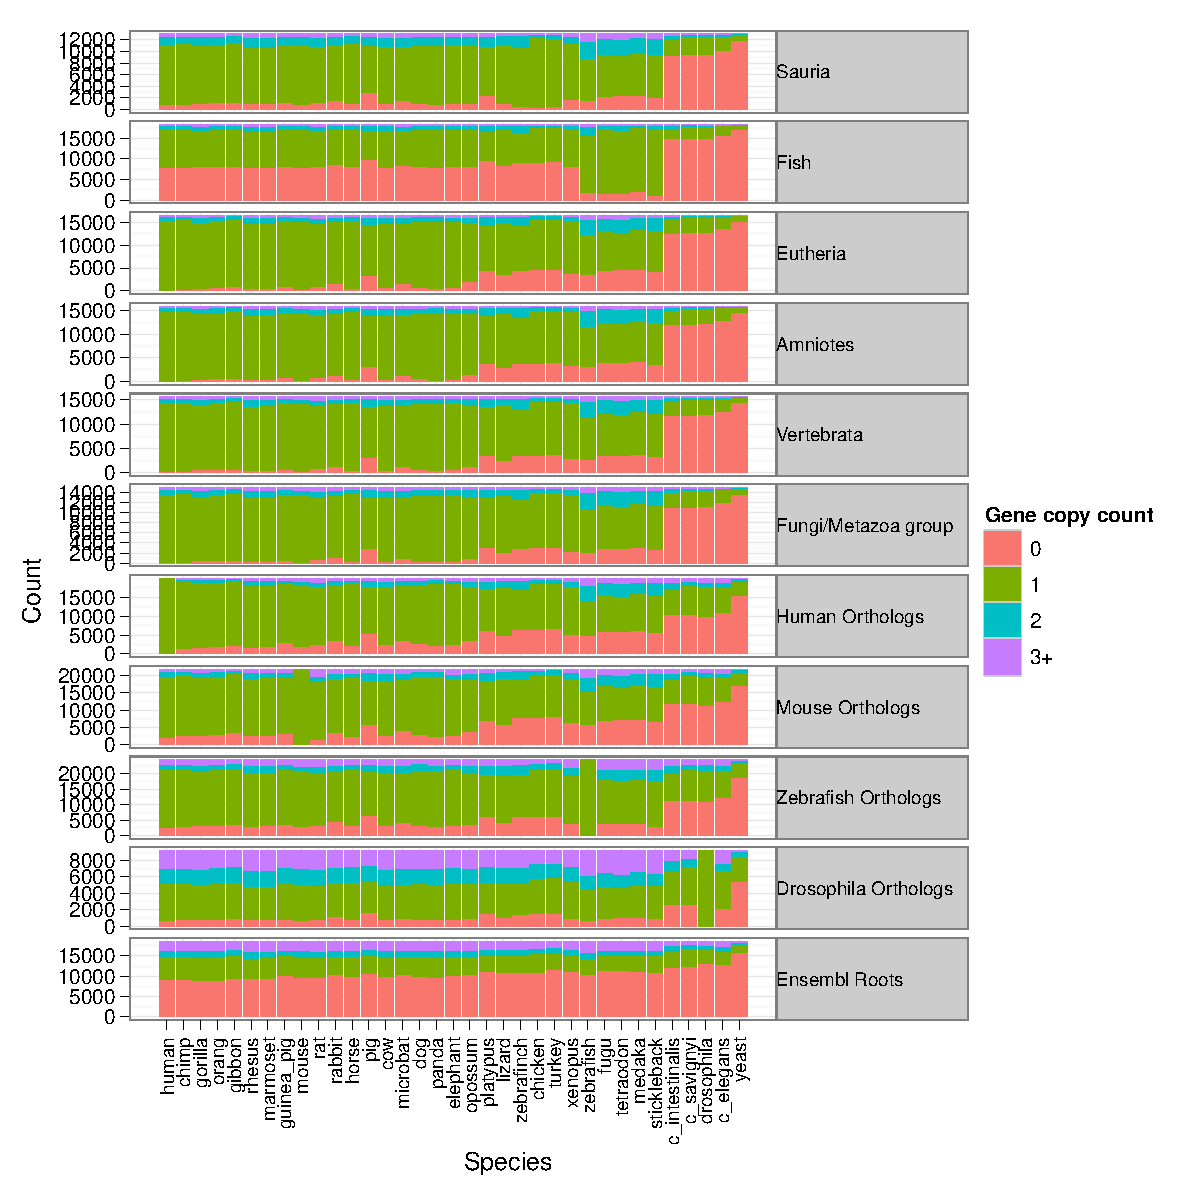
\includegraphics[scale=0.8]{Figs/ortholog_stacked_bar.pdf}
\caption{Taxonomic distribution of gene copy counts for different
  \subtr methods. The numbers of trees containing 0 (red), 1 (green),
  2 (blue) or more than 3 (purple) sequences from each species are
  shown as stacked colored bars. The Ingroup and Subgroups methods
  were omitted for clarity, as were species with low-coverage
  genomes. Note that the y-axis scale is not the same for each panel.}
\label{ortholog_stacked_bar}
\end{figure}

In the end, the set of Eutheria \subtr{}s was chosen as the final set
for use in the downstream evolutionary analysis, due to the slightly
larger number of trees and better coverage of human genes in the
Eutheria set compared to the other Outgroup methods. The distribution
of tree sizes for the Eutheria set of \subtr{}s is shown in Figure
\ref{ensembl_euth_hist} and the full taxonomic distribution of copy
counts is included in Figure \ref{ortholog_euth_dups}.

\begin{landscape}
\begin{figure}
\centering
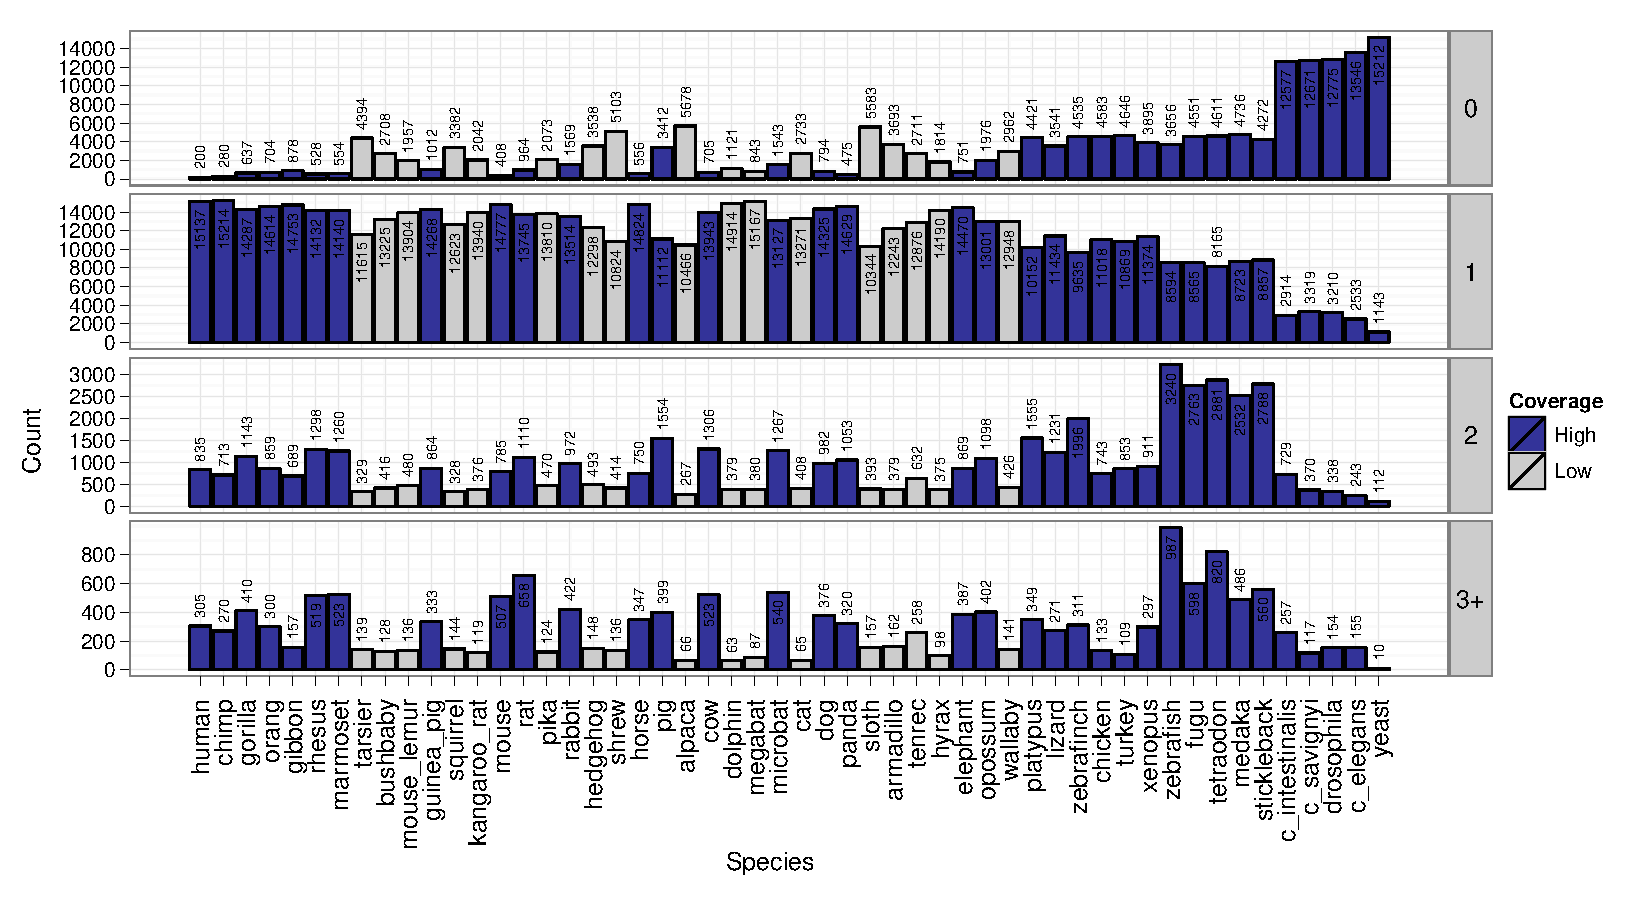
\includegraphics[scale=0.9]{Figs/ortholog_euth_dups.pdf}
\caption{Taxonomic distribution of gene copy counts for the Eutheria
  \subtr{}s. The number of trees containing 0, 1, 2 or more than 3
  sequences from each species is shown. Bars are colored blue and gray
  for species with high- and low-coverage genomes, respectively. Note
  that the y-axis scale is not the same for each panel.}
\label{ortholog_euth_dups}
\end{figure}
\end{landscape}

\begin{figure}
\centering
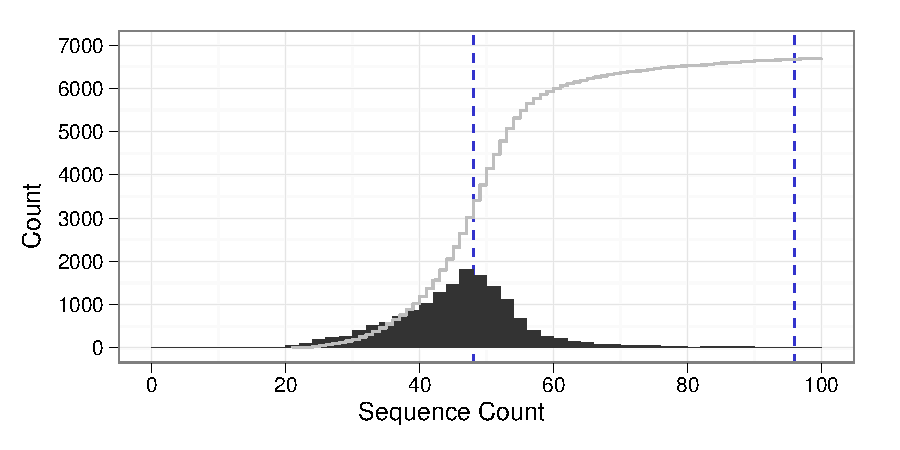
\includegraphics[scale=0.9]{Figs/ensembl_euth_hist.pdf}
\caption{Sequence counts for the set of \subtr{}s identified using the
  Eutheria clade taxonomic coverage constraint. Black bars show a
  histogram of sequence counts in bins of width 2, a gray line shows
  the cumulative fraction of sequences contained within trees of that
  size or smaller, and dashed blue lines are drawn at integral
  multiples of 48, the number of vertebrate species within
  Ensembl. The XYZ trees with more than 100 sequences are not shown.}
\label{ensembl_euth_hist}
\end{figure}

\todo{Find num. of Eutherian trees w/ more than 100 seqs}

%************************************************
\chapter{Patterns of sitewise selection in mammalian genomes}
\label{ch_mammals1}
\acresetall
%************************************************

\section{Introduction}

This chapter describes the use of sitewise evolutionary estimates to
characterize the genome-wide distribution of selective constraint in
mammals and within the major mammalian superorders. I apply the
\ac{slr} test, which was introduced in Chapter \ref{ch_intro} and
evaluated in Chapter \ref{ch_indels1}, to the set of orthologous gene
trees from Chapter \ref{ch_orthologs} to estimate statistics measuring
\sw selective constraint in several groups of \mammln species. Both
this chapter and Chapter \ref{ch_mammals2} are concerned with the
analysis of these \sw data: here I will analyze the overall
distribution of constraint observed in several groups of mammalian
genomes, and Chapter \ref{ch_mammals2} will apply these \sw data to
identify genes, biological processes and protein domains with the
strongest genome-wide enrichment for signals of positive selection.

The first section of this chapter describes the filtering and
alignment of mammalian orthologs and introduces a protocol for
filtering \sw estimates of selective pressures. Although the
simulations from Chapter \ref{ch_indels1} showed that sequences with
mammalian-like divergence levels showing biological patterns of
insertion and deletion can be aligned without introducing many false
positive \acp{psc}, the analysis of real sequence data involves many
potential non-biological sources of alignment error. A sequenced and
annotated genome is not a piece of observed data; rather, it is the
result of a succession of inferences, each one of which involves
potential errors and biases. Errors may arise during the sequencing of
DNA bases, assembly of genomic fragments, and annotation of
gene-coding regions; each of these steps has been previously
highlighted as an important source of error in the large-scale
analysis of genomic alignments
\citep{Schneider2009,Mallick2009,Milinkovitch2010,Hubisz2011}. As
such, care was taken in this study to design and evaluate a variety of
filters to reduce the probability of yielding misleading results.

The second portion of this chapter presents an analysis of the global
distribution of mammalian selective constraint, using \sw estimates to
identify sites evolving under purifying and positive selection in
different groups of species. In parallel with the major goal of the
\ac{mgp} to better identify and understand the nature of evolutionary
constraint across mammalian genomes, the purpose of this analysis was
to better characterize the distribution of evolutionary constraint
within mammalian protein-coding regions. Thus, a major question was
what proportion of protein-coding material has been evolving under
purifying, neutral, or positive selection in mammals. Proteins are
well understood to evolve under strong purifying constraint due to
their functional importance \citep{Fay2003}, but some regions of
proteins, such as disordered regions between two well-folded domains,
may evolve under relaxed constraints. Furthermore, positive selection
of beneficial substitutions can also play a role in shaping the
evolutionary history of proteins \citep{Pal2006}. There has thus been
great interest in understanding the role of adaptive evolution in
shaping the genes and genomes of mammals and primates, but different
studies have produced widely varying estimates of the number of genes
subject to positive selection \citep{Ellegren2008,MarquesBonet2009a}.

While most genome-wide analyses of selective constraint have focused
on the gene as the unit of analysis
\citep{Nielsen2005,Sequencing2005a,Kosiol2008}, this chapter adopts a
primarily \sw approach, presenting distributions of \sw estimates
aggregated across all sites from all genes included in the
analysis. The use of explicitly \sw estimates allowed for various
types of filtering to be applied, removing sites sites from the
dataset according to different filtering criteria. Different \sw
filters could be applied without the computationally expensive step of
re-estimating evolutionary parameters, allowing for the impact of
various filters on the amount of inferred positive and purifying
selection to be quickly and flexibly estimated.

%The second, more subtle goal of this analysis was to place the
%distribution of selective pressures implied by the \sw analysis within
%the context of previous population genetic and comparative
%studies. Many population genetic studies have analyzed the
%distribution of selective pressures resulting from mutations in
%protein-coding regions, known as the \ac{dfe}. Analyses of variation
%data from \emph{Drosophila} have found that relatively few amino acid
%substitutions in \emph{Drosophila} are effectively neutral, while up
%to 50\% have apparently been due to positive selection
%\citep{Loewe2006,EyreWalker2007}; similar studies based on variations
%in humans have indicated a much lower fraction of positively-selected
%substitutions in our recent evolutionary history
%\citep{EyreWalker2006a,Boyko2008}. This is in line with the
%expectation, based on population genetic theory, that species with
%higher effective population sizes experience more effective natural
%selection \citep{EyreWalker2007}. As \emph{Drosophila} has
%historically had a much larger effective population size than humans
%and most mammals (e.g., on the order of 10$^{6}$ for \emph{Drosophila}
%vs. 10$^{3}$ for humans), one would expect to see more neutral
%evolution, and less purifying and positive selection, in human
%protein-coding regions.

%Although there is a strong theoretical connection between the \ac{dfe}
%commonly from population genetics and the \dnds ratios more commonly
%estimated in comparative analyses, only one study, performed by
%Nielsen and Yang \citeyearpar{Nielsen2003}, has explicitly estimated
%the \ac{dfe} using data from fixed differences between species. Using
%data from primate mitochondrial genomes, Nielsen and Yang found that a
%variety of two-parameter distributions for the \ac{dfe} fit the
%dataset equally well and that none of the best-fit distributions
%contained a large amount of probability mass within the range of
%purely neutral or beneficial selection coefficients; most of the
%distribution was contained within the range of moderately deleterious
%selection coefficients (e.g., $-3<S<-1$, corresponding roughly to
%\dnds values between 0.2 and 0.6). Unfortunately, no attempt has since
%been made to use comparative data to estimate the \ac{dfe}; as a
%result, one goal of this analysis was to determine whether \sw
%estimates could successfully be used to infer the \ac{dfe}. Though the
%methods I employed for this analysis differed strongly from the
%approach of Nielsen and Yang, a comparison to their results could
%validate the use of \ac{slr} for estimating the \ac{dfe}. Furthermore,
%it would be interesting to understand whether the differences in
%historical effective population sizes between mammalian subgroups,
%which have been shown repeatedly to affect overall \dnds levels in
%primates versus rodents \citep{Kosiol2008,Ellegren2009}, has a
%detectable impact on the \ac{dfe} inferred from comparative
%data. Although the effective population size differences between
%mammalian subgroups are far smaller than the difference between
%mammals and species like \emph{Drosophila}, a comparison of the
%\ac{dfe} from different mammalian groups could be used to evaluate how
%strong of an impact the effective population size has on the
%proportion of protein-coding sites subject to varying levels of
%natural selection.

\section{Data quality concerns: sequencing, assembly and annotation error}
%\subsection{The impact of sequencing errors on error rates in detecting positive selection}
\label{sec_error_impact}

The possibility that erroneously-aligned sequences might cause false
positives in the detection of sitewise positive selection was a major
concern for this analysis, especially given the \lcv nature of the 20
genomes sequenced by the \ac{mgp}. A number of issues relating to the
impact of \lcv genomes on the detection of orthologs were discussed in
Chapter \ref{ch_orthologs}; here, the focus was on how, after
orthology has been inferred, sequences from \lcv genomes may
contribute to the false detection of positive selection. Although the
\slr test and other \sw \ml methods have been shown to be conservative
in their identification of positively selected sites under most
conditions, even when the amount of data is low or the null model is
violated \citep{Anisimova2002,Anisimova2003,Massingham2005}, most
evolutionary analyses are based on the assumption that all sites
within an alignment column are truly homologous. This assumption can
be violated in a number of ways, resulting in misalignment.
%Here misalignemnt will be
%defined as the incorrect placement of \nhom nucleotides into the same
%column of a multiple sequence alignment.

In Chapter \ref{ch_indels1} I explored misalignment resulting from
errors in reconstructing the evolutionary history of sequences
evolving with insertions and deletions. Simulations showed that
\prankc alignments contained little misalignment and caused few false
positives in the \sw detection of positive selection. However,
biological insertions and deletions are not the only potential source
of misalignment. An additional concern was the potential for errors
resulting from the inclusion of erroneous or \nhom sequence regions
within the mammalian orthologs. As the \lcv genomes were not assembled
into chromosomes and contained large amounts of missing sequence, the
likelihood of miscalled bases, spurious insertions or deletions, or
shuffled regions due to mis-assembly was relatively high
\citep{Green2007}. Most aligners were not designed to deal with these
types of errors, so they may be expected to result in excess
misaligned regions.

%Since \ac{slr} uses a model which assumes independence between amino
%acid sites, the effect of any type of misalignment on the resulting
%inference will be largely, but not entirely. independent between
%neighboring codons. In reality, errors will have some impact on other
%sites through the estimation of parameters which are common to all
%sites.

% . Thus, one may first consider the
%effect---in isolation---of a single spuriously-assigned homologous
%codon on the \ml estimation of \omg. Two distinct situations can be
%encountered: first, the case where a single sequence error causes one
%spurious nucleotide substitution within a codon, and second, the case
%where one or multiple sequence or assembly errors cause multiple
%spurious substitutions within a codon. Single spurious nucleotides,
%such as miscalled bases, would add noise to the estimation of \omg,
%but as a whole they would not be expected to cause false positive
%\acp{psc}. If we assume no large difference between the natural
%mutational process and the process that caused the erroneous mutation
%(e.g., a random distribution across codon positions and no bias in the
%identity of the miscalled base) then the effect would be to shift the
%estimated \omg in the branch containing the error towards 1. This is
%because, on average, isolated miscalled bases would appear the same as
%a neutral substitution process, inflating the estimated substitution
%rate but not affecting the relative \nsyn and \syn rates.

%In contrast to single spurious substitions, codons with multiple
%erroneous bases in one species may produce strongly elevated inferred
%substitution rates and \omg estimates. This is due to the necessity of
%the codon model implemented in SLR to infer a multi-step path of
%single substitutions between the two codons on either side of a given
%evolutionary branch. The exact \ml path estimated between two
%completely non-homologous codons depends on the estimated codon
%frequencies, the branch length separating the two sequences, and the
%nature of the process causing misalignment of nonhomologous codons,
%but in general it would be reasonable to expect a greater number of
%false positive \acp{psc} resulting from codons with multiple erroneous
%bases than from codons with single errors due to the necessary
%inference of a multi-step path between codons with multiple nucleotide
%differences.

%Given the potentially greater impact of codons with multiple errors,
%the propensity of each of the common sequencing error types identified
%above (miscalled bases, spurious indels, and
%shuffled/repeated/collapsed regions due to mis-assembly) to cause
%single or multiple errors within codons could strongly affect its
%impact on the sitewise detection of positive selection. On its own, a
%miscalled nucleotide base would obviously result in a single spurious
%substitution. However, low-quality bases tend not to be uniformly
%distributed among or within sequence reads \citep{Kircher2009},
%leading to an increased probability of multiple errors within a codon
%resulting from miscalled bases. Spurious indels within coding regions
%may be even more likely than miscalled bases to cause multiple errors
%within a codon due to the potential for creating frameshift
%artifacts. Assembly errors, which result in larger-scale structural
%errors including missing, repeated, shuffled or inverted sequence
%regions \citep{Jaffe2003}, are especially prone to producing codons
%with multiple erroneous substitutions due to the large amount of
%contiguous sequence data being misplaced.

%For detecting positive selection, the specific test used and the
%branch lengths separating the species being tested may also have an
%impact on the prevalence false positives resulting from sequence
%errors. Sequence errors should only substantially affect the
%estimation of \nsyn and \syn substitution rates along the terminal
%lineage leading to the erroneous sequence data; thus, the potential
%impact of sequencing error on the inference of a positively selected
%site or gene can be estimated by considering the potential impact of
%an inflated rate of \nsyn substitution along the terminal branch on
%the inference of positive selection with a given test. Both the
%branch-site test for positive selection (which was not used in this
%analysis) and the sitewise tests for positive selection (including
%\pamlEight and \slr) are
%sensitive to erroneous substitutions occurring at individual alignment
%columns, with the major difference between the two types of test being
%that the branch-site test is highly sensitive to substitutions along
%the foreground branch(es) being tested for positive selection, while
%sitewise tests only measure the signal for positive selection across
%the entire evolutionary tree.

%For the branch-site test, the potential effect of sequencing error
%should depend on the location and length of the foreground branch(es):
%if the terminal branch leading to the spurious sequence is within the
%foreground, and especially if it represents a sizeable portion of the
%overall foreground branch length, then false positives could easily
%result; if, however, the terminal branch is outside of the foreground,
%then it would have little direct impact on the \fpr of the branch-site
%test aside from adding noise to the estimation of parameters in the
%non-foreground branches of the tree.

%For site-based tests such as \slr, the effect of sequencing error
%should be independent of the position of the terminal branch within
%the tree, depending more on the magnitude of \nsyn substitution rate
%elevation resulting from the sequence error and the fraction of total
%branch length covered by the ``erroneous'' terminal branch within the
%phylogenetic tree being studied. It would be difficult to consider
%each of these factors (the terminal branch length and the magnitude of
%\nsyn substitution rate elevation) in isolation due to their
%non-independence: sequence errors in a short terminal branch may yield
%a strongly elevated \nsyn substitution rate, but the impact on the
%overall inference of positive selection may be limited as a result of
%the short branch length. On the other hand, the same erroneous
%sequence in a species with a longer terminal branch would likely cause
%a smaller elevation in the \nsyn substitution rate (due to the higher
%expected number of substitutions along a longer branch) yet the impact
%of such an elevated rate on the sitewise inference would be
%proportionally greater due to the higher branch length. A reasonable
%hypothesis would be that these opposing factors would effectively
%cancel each other out in the \ml calculations. In either case, the
%expectation that a phylogeny with a greater proportion of its branch
%length within terminal branches (which, in contrast to internal
%branches, may contain spurious substitutions resulting from sequencing
%errors) would be more prone to false positives should still hold.

%To summarize, the expected effect of alignment errors on the sitewise
%detection of positive selection should be minimal when using a good
%aligner and analysing data within vertebrate divergence levels, but
%the number of false positives resulting from sequence errors depends
%on a number of factors including the frequency, spatial clustering,
%and terminal branch length associated with sequencing, assembly and
%annotation errors.

The impact of these types of errors on detecting positive selection at
any given codon should depend on the model used to infer selection,
the number and identify of the \nhom nucleotides placed in the same
aligned codon, and the branch length leading to the sequence
containing the misaligned bases. Misalignment of multiple nucleotides
in the same codon would tend to produce more false positives than
single-nucleotide errors, and misalignment in sequences or trees with
shorter branch length may have an overall greater impact on the
estimated \nsyn substitution rates.

\subsection{Empirical evidence for a strong impact of sequencing, assembly and alignment error}

Simulation studies could improve our understanding of the relative
potential of different types of sequencing errors to introduce false
positives in downstream analyses, but the absolute frequency and
pattern of such errors would still be difficult to predict without a
reliable model for their generation. This is especially true for
larger-scale errors from mis-assembly or mis-annotation, which are
less easily modeled than some other types of error, e.g., base
calling, and could have potentially more significant negative
effects. Instead, an empirical approach seems more appropriate for
quantifying the false positives resulting from these types of sequence
errors. Two recent empirical studies in mammals provided convincing
evidence that sequence, alignment and annotation errors can increase
the number of false positive \psg{}s in the branch-site test for
positive selection (\citet{Zhang2005}; introduced in Chapter
\ref{ch_intro}).

\citet{Schneider2009} performed a genome-wide
scan for positive selection in the terminal branches of 7 mammalian
genomes using the branch-site test and analysed the fraction of
\psg{}s within subsets of high- or low-quality genes according to
three sequence and alignment quality metrics. They found that the
fraction of \psg{}s was significnatly higher for genes exhibiting
lower quality sequence, annotation and alignments, with genes in the
highest-quality and lowest-quality categories showing a 7.2-fold
difference in the inferred fraction of \psg{}s
\citep{Schneider2009}. This observation provided evidence of a
correlation between the chosen quality metrics and the tendency of an
alignment to exhibit positive selection. It did not necessarily imply
causation, however, as the same result might have been observed---even
in the absence of sequence error---if some biological properties of
the true \psg{}s caused them to yield lower quality metrics than
non-\psg{}s. Looking at the three metrics used in their study
(sequencing coverage, gene annotation status, and alignment quality
according to the heads-or-tails method), it is plausible that
properties associated with elevated \omg ratios and positive
selection, such as recent gene duplication
\citep{Beisswanger2008,Studer2008,Casola2009}, high GC content
\citep{Ratnakumar2010} or functional shifts \citep{Storz2008,Wang2001}
might have had an error-independent effect resulting in a higher
proportion of \psg{}s in low-scoring categories. The heads-or-tails
method has also been shown to be inappropriate for estimating
alignment uncertainty \citep{Fletcher2010}, so the authors' results
based on this measurement were questionable. Despite these criticisms,
overall \citet{Schneider2009} provided good evidence that some
measurable sources of error may be contributing to excessive estimates
of branch-specific positive selection in mammals.

\citet{Mallick2009} took a different approach to the same problem by
performing a careful resequencing and reassembly of the chimpanzee
genome (the initial assembly of which had lower coverage and lower
quality than the human genome) and re-analysing the evidence for
positive selection along the chimpanzee lineage in 59 genes which had
been identified as chimpanzee \psg{}s by
\citet{Bakewell2007}. \citet{Mallick2009} were concerned that the
finding by \citet{Bakewell2007} of a larger proportion of \psg{}s in
chimpanzee than in human was the result of the lower-quality
chimpanzee genome rather than a biologically significant difference in
levels of adaptation. \citet{Mallick2009} found that the vast majority
of \psg{}s identified in two previous studies showed no evidence for
positive selection when using their reassembled and higher-coverage
version of the chimpanzee genome. This suggested that the original 4x
coverage chimpanzee genome contained a number of sequencing and
assembly errors leading to false inferences of positive selection. The
authors' detailed analysis of 302 codons with multiple spurious \nsyn
substitutions in the original chimpanzee assembly showed roughly
comparable contributions from sequence error (explaining 23\% of
codons), assembly error (14\% of codons) and local alignment error
(30\% of codons).

Taken together, the results of \citet{Schneider2009} and
\citet{Mallick2009} provide strong evidence in support of the
hypothesis that errors in sequencing, assembly, annotation and
alignment can result in strongly elevated inferred \omg values when
using sensitive tests for detecting positive selection. Furthermore,
the detailed identification and quantification of error sources
performed by \citet{Mallick2009} shows how important each potential
source of error would be in the detection of positive
selection. Although both of these studies used the branch-site test
for detecting positive selection while the current analysis focused on
detecting \sw positive selection throughout the tree, their results
could be expected to generalize well enough to guide the design of
filtering methods for the present \sw analysis.

Three filtering steps were implemented to help identify and remove
sequences and alignment regions potentially subject to the errors
noted above: filtering out low-quality sequence, removing gene
fragments and recent paralogs, and identifying alignment regions with
extremely high numbers of clustered substitutions.

\subsection{Filtering out low-quality sequence}

I first applied a conservative filter to the set of input sequences
based on sequence quality scores associated with each genome for which
such scores were available. Most automated genome assembly pipelines
output a set of Phred quality scores alongside the identified genome
sequence, with one Phred score per base ranging in value from 0 to
50. These scores represent the probability, calculated by the
sequencing and/or assembly program, that a given base call is
incorrect. This probability is concisely expressed as the negative
base-10 logarithm of the probability of an error multiplied by 10, or
$Q=-10log_{10}P$, where $Q$ is the Phred score and $P$ is the
probability of an incorrect base call \citep{Cock2010}.

\ens does not store quality scores from its source genome assemblies,
so Phred quality scores were downloaded for all \lcv genomes where
Phred-like quality scores were made publicly available alongside the
genomic sequence. Most quality scores were provided as a single file
in FASTA format with one string of numerical scores per assembled
contig.

A suitable score threshold for filtering coding regions was chosen
based on a study by \citet{Hubisz2011}, who performed a detailed
analysis of Phred quality scores and actual error rates in \lcv
mammalian genome assemblies by comparing the \lcv assemblies to
matched regions of high-quality sequence from the ENCODE comparative
genomics dataset \citep{Birney2007}. They also identified a strong
correlation between Phred scores and actual error rates for scores
below 25, indicating that the scores were accurate predictors of the
true error rate in this range. Error rates did not decrease
significantly at scores above 25, however, suggesting that the use of
an extremely high Phred score threshold would only minimally reduce
error levels below those obtained with a moderate
threshold. Furthermore, \citet{Hubisz2011} noted that 85\% of the
bases in the low-coverage mammalian genomes contain very high Phred
scores ($>45$) and only 4\% have low scores ($<20$).

Based on these observations, a score threshold of 25 was chosen as a
reasonable trade-off between the potential benefit of removing
miscalled bases and the potential cost of masking out correctly
sequenced bases. For each protein-coding sequence with quality scores
available, a ``minimum score'' approach was used to filter out whole
codons: all codons containing one or more nucleotides with a score
below 25 were masked out with three ambiguous nucleotides, `NNN'.

%The expected proportion of filtered nucleotides could be calculated
%from the fraction of bases below the Phred score threshold of
%25. According to Hubisz et al. \citeyearpar{Hubisz2011}, approximately
%5\% of bases in low-coverage mammalian genomes contain Phred scores
%below 25. The worst case scenario (e.g., the worst case in terms of
%the number of high-quality bases being masked as a result of using the
%minimum score approach) would be if only one base per codon had a
%score below the threshold. In that case, an expected 15\% of
%nucleotides would be filtered, since 3 bases would be masked for every
%low-quality base. However, the distribution of low-quality bases is
%likely highly clustered, due to the uneven distribution of
%repetitiveness and GC content as well as the tendency for uncertain
%base calls to occur towards the end of sequence reads (all of which
%are known to affect read coverage and assembly performance,
%e.g. \cite{Teytelman2009}). A more clustered distribution of
%low-quality bases would cause fewer high-quality bases to become
%masked by the minimum score approach, reaching the limit of an
%expected 5\% total filtered bases if low-quality bases always occurred
%in groups of three and were positioned along the boundary of codon
%triplets. Thus, anywhere from 5\% to 15\% of nucleotides from
%low-coverage genomes were expected to be filtered by this approach.

\begin{figure}
\centering
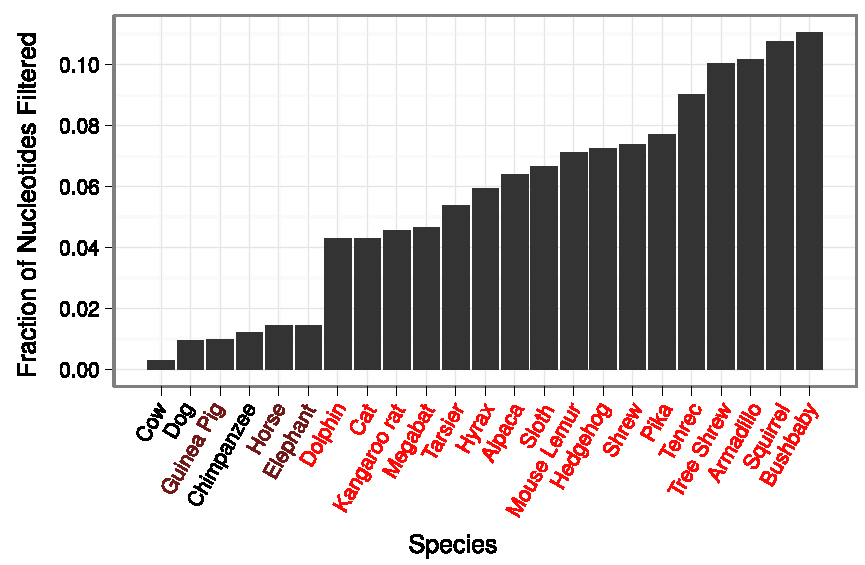
\includegraphics[scale=0.9]{Figs/qual_filter_hist.pdf}
\caption{The fraction of nucleotides masked from protein-coding
  regions of mammalian genomes based on low predicted sequence
  quality. For genomes with Phred sequence quality scores available,
  all codons containing any nucleotides with a Phred score $<25$ were
  masked with `N's. Each bar shows the fraction of nucleotide
  sequences (compared to the total number of coding nucleotides from
  each genome) which were masked. As in Figure \ref{fig_ncbi_tree},
  high-coverage genomes are labeled in black, \lcv genomes are labeled
  in red, and guinea pig and elephant---whose genomes were originally
  sequenced at 2x coverage but were later ``topped up'' to 7x
  coverage--are labeled in dark red. Phred scores were unavailable for
  most high-coverage genomes, and Phred scores for wallaby were unable
  to be used due to mismatched assembly versions (see text).}
\label{filtered_qual_bars}
\end{figure}

The above filtering scheme was applied to all coding sequences from
each genome for which quality scores were available, which included
all of the \lcv genomes (except for wallaby) and six high-coverage
genomes. Unfortunately, the \lcv wallaby genome was not filtered based
on sequence quality due to a mismatch in the sequence identifiers used
by \ens and those found in the quality score files made available for
download; wallaby was not one of the 29 species included in the
original \ac{mgp} analysis, but this error has been marked for
correction in a future version of the 38-species analysis. Note also
that the guinea pig, rabbit, microbat, horse and elephant genomes were
originally sequenced at low 2x coverage for the \ac{mgp}, but they
since underwent additional sequencing to produce high-coverage 7x
assemblies (these species are labeled in dark red in Figure
\ref{fig_ncbi_tree} from Chapter \ref{ch_orthologs}). These
higher-coverage assemblies were used for release 63 of \ens and for
the present analysis. Phred scores for the high-coverage guinea pig,
horse, and elephant assemblies were used for filtering here, but Phred
scores for the high-coverage rabbit and microbat assemblies were not
provided by the sequencing institutions.

The fraction of nucleotides filtered from each genome is shown in
Figure \ref{filtered_qual_bars}. Genomes with high-coverage assemblies
contained fewer bases with low Phred scores, resulting in 1-2\% of
nucleotides being filtered, while the bulk of low-coverage genomes
resulted in 4-8\% of nucleotides being filtered.  Five genomes
(bushbaby, squirrel, tree shrew, armadillo and tenrec) showed a
noticeably higher proportion of low-quality bases, with 9-11\%
nucleotides being filtered out. The distribution of filtered
nucleotide proportions confirmed the expectation based on
\citet{Hubisz2011} that 5-10\% of nucleotides would be filtered using
a Phred score threshold of 25, and the variation in filtered
nucleotide proportions between different \lcv species showed that
despite the uniform 2x coverage of the \lcv mammalian genomes,
different assemblies varied widely in their distributions of sequence
quality scores within coding regions.

The lack of publicly available sequence quality scores for most
high-coverage genomes was lamentable, especially for the
closely-related primates. Taking chimpanzee as an example
high-coverage genome with quality scores available (although it may
have an exceptionally error-prone genome sequence
\citep{Mallick2009}), the procedure described above resulted in
331,737 nucleotides, or roughly 1\% of all protein-coding nucleotides,
being masked. Clearly some of those masked nucleotides were of lower
quality and some were of higher quality (i.e., high-quality
nucleotides removed on account of being within a masked codon). But if
one assumes a constant error probability among masked nucleotides of
$3.16e-3$ (corresponding to the $Q=25$ threshold), then an expected
1,049 of the masked chimpanzee nucleotides contained sequencing
errors. An equivalent calculation for bushbaby, a \lcv primate genome,
yielded 2,694,054 filtered nucleotides and 8,519 expected sequencing
errors.

These numbers may be evaluated in terms of signal and noise, where
true substitution events are the desired evolutionary signal and
errors are noise. To estimate the amount of ``signal'' present in each
species' terminal lineage, the genome-wide set of filtered alignments
was used to infer substitution events along each branch (the methods
used for this are described in Section
\ref{section_windows_clustered_subs}), yielding 85,368 substitutions
along the chimpanzee branch and 892,890 substitutions along the
bushbaby branch. Comparing the inferred signal to the estimated noise
in each of these example genomes, one finds that for each true
lineage-specific substitution there were approximately 0.0095 expected
errors in the bushbaby genome and 0.0123 expected errors in the
chimpanzee genome. Thus, even though the chimpanzee genome was
sequenced to 6x coverage while bushbaby was only sequenced to 2x
coverage, the unmasked chimpanzee genome contained perhaps a lower
``signal-to-noise'' ratio within coding sequences than the unmasked
bushbaby genome.

These calculations were in general agreement with a study by
\citet{Taudien2006} which appraised the extent to which errors in an
earlier \ac{wd} version of the chimpanzee genome affected the
comparative analysis of coding regions. Although the overall error
rate of the \ac{wd} sequence was low, they found that up to 20\% of
the exonic sequence differences between human and chimpanzee were
false positives resulting from errors in the chimpanzee sequence. When
a quality score threshold of $Q>20$ was used, however, the proportion
of false positives decreased markedly to 8\% \citep{Taudien2006}. The
issue of sequence quality will be considered again in Chapter
\ref{ch_gorilla}, where I examined the impact of sequence filtering on
the estimation of genome-wide \dnds values within primates.

\subsection{Removing recent paralogs}
\label{sec_removing_paralogs}

%As discussed in Section \ref{section_quantifying_paralogous}, 

Chapter \ref{ch_orthologs} discussed a number of issues relating to
the identification of homologous protein-coding sequences, and a set
of largely orthologous gene trees was collected. The relatively low
amount of sequence divergence within mammals suggested that the
probability of erroneous inclusion of altogether non-homologous
sequences was low, but the existence of paralogous relationships
within the alignments used for \sw analysis was still a concern.

The inclusion of paralogous gene relationships in a large-scale
analysis of orthologous gene evolution may produce unwanted signals of
adaptive evolution following gene duplication \citep{Lynch2000},
artifacts resulting from gene conversion \citep{Casola2009} or biases
due to lineage-specific family expansion, a process which is
relatively common in mammalian gene families \citep{Gu2002}. As a
result, it has traditionally been considered important to filter out
recently-duplicated genes (e.g., genes duplicated after the
whole-genome duplication event in the vertebrate ancestor) in
large-scale evolutionary analyses. Previous genome-wide scans for
positive selection involving six or fewer mammalian genomes have
either required strict one-to-one orthology
\citep{Clark2003,Nielsen2005} or allowed very limited numbers of
recent duplications in specific lineages \citep{Kosiol2008}. With
larger numbers of species included in a phylogenetic analysis,
however, the requirement of strict one-to-one orthology becomes
increasingly untenable: if gene duplications and deletions occur
randomly in time, then the probability of observing at least one such
event in a given gene family should increase linearly with the amount
of branch length covered by the tree. The requirement of one-to-one
orthology would result in fewer genes being available for analysis as
more species are included, which is clearly an undesirable trend. As
an alternative to ignoring genes which do not satisfy the requirement
of strict orthology, I developed an approach, described below, for
handling recently duplicated genes by removing the more divergent or
shorter paralogous copy from the gene tree.

%Before describing the method for duplications, it is worth making a
%point about gene deletions. Specifically, I note that gene deletions
%can complicate the branch-specific detection of positive selection,
%but they should not have a detrimental effect on tests for selection
%across the entire tree. The effect on branch-specific tests results
%from the merging of multiple ancestral branches into one. Take for
%example the inference of mutations along the evolutionary tree of
%human, chimpanzee and gorilla, which contains two internal nodes:
%$HC$, the human-chimpanzee ancestor, and $HCG$, the
%human-chimpanzee-gorilla ancestor. When sequences from all species are
%present, mutations can be separately identified as occurring along the
%branch from $HCG$ to $HC$ and along the branch from $HC$ to the human
%sequence, allowing for a test to differentiate between a signal of
%adaptive evolution in one branch or the other. For a gene which was
%deleted in chimpanzee those two branches become effectively merged
%into one, and mutations can only be inferred to have occurred between
%$HCG$ and the human sequence. The time-specificity of estimated
%evolutionary rates is thus reduced, and when the identity of the
%branch along which \syn and \nsyn mutations have occurred is important
%to a test for positive selection, this difference can complicate the
%interpretation of results. Acknowledging this effect,
%\citet{Kosiol2008} used a different set of orthology requirements for
%each branch-specific test for positive selection performed. When the
%test for positive selection does not depend on the identity of
%specific branches in the tree, however, a gene deletion would only
%serve to reduce the total amount of branch length available for
%inference. As long as the branch leading to the deleted species did
%not comprise a large portion of the total branch length, the effect of
%gene deletion on the results of tree-wide tests for selection should
%be minimal.

%Turning back to gene duplications,

An additional complicating factor in the current analysis was the
concern that many of the apparent gene duplications might actually be
artifacts of the annotation of \lcv genomes. Each \lcv genome assembly
is highly fragmented, meaning that it contains many short sequence
segments that were unable to be assembled into chromosome-sized
sequences due to missing intervening sequence data. Sometimes the
exons of a gene spanned the boundaries of these sequence segments,
causing different parts of a gene to exist on different segments. The
\ens annotation pipeline was not designed to merge gene annotations
across different sequence segments, so each part of a gene residing on
multiple sequence segments would be annotated as a separate shortened
gene. These shortened genes would be treated as independent proteins
by the \cmp pipeline, likely being placed at very similar positions in
the gene tree due to each sequence having been derived from a gene
with a single correct evolutionary position. This result might not be
detrimental to sitewise analysis in itself, as each shortened gene may
end up being correctly aligned and provide useful information to the
alignment. However, a number of factors, including the low quality of
genomic sequence and assembly within these shortened genes, problems
with aligning small fractions of a gene against complete sequences and
the potential for incorrect placement of fragmented sequences within
the gene tree, made it desirable to remove the shortest of these gene
fragments.

Sequence divergence was the other criterion used to select which
paralogous copy of recently-duplicated genes to retain. Models of
evolution after gene duplication have tended to predict that one of the
duplicate copies retains the ancestral function (and its associated
pattern of evolutionary constraint) while the other duplicate
experiences relaxed constraint followed by either degradation or
functional diversification \citep{Han2009}. Thus, the least-diverged
copy of a recently duplicated gene should be the one most likely to
have retained the pattern of evolutionary constraint shared among the
mammalian species being examined in this study.

The protocol I implemented for filtering apparent paralogs used both
gene length and sequence divergence to identify which gene among a set
of apparent paralogous copies was most suitable to retain for
analysis. Gene length was used primarily to discriminate spuriously
shortened genes from true genes, and sequence divergence was used to
distinguish between more- and less-diverged paralogs. First, the mean
pairwise sequence distance was calculated between each putative
paralog and all other sequences in the gene tree, resulting in one
mean pairwise distance estimate per putative paralog (hereafter
referred to as the mean distance). For these distance calculations,
the coding sequence alignments provided by \ens \cmp and the JC69
nucleotide model were used to estimate distances. Second, the ratio of
the sequence length of each putative paralog to the mean sequence
length across the tree (hereafter referred to as the length ratio) was
also calculated.

Genes were grouped by species within each gene tree, and any group of
twp or more genes from the same species was considered to be a set of
putative paralogs. Within each set of putative paralogs, a single gene
was chosen to be retained for evolutionary analysis based on three
rules applied in the following order: (1) if only one sequence had a
length ratio above 0.5 and all others had a length ratio below 0.5,
the longest sequence was kept; (2) if one sequence yielded a mean
distance below the others, that sequence was kept; (3) if all mean
distances were identical then the longest sequence was kept, or if all
mean distances and length ratios were equal, an arbitrary choice was
made.

\begin{figure}
\centering
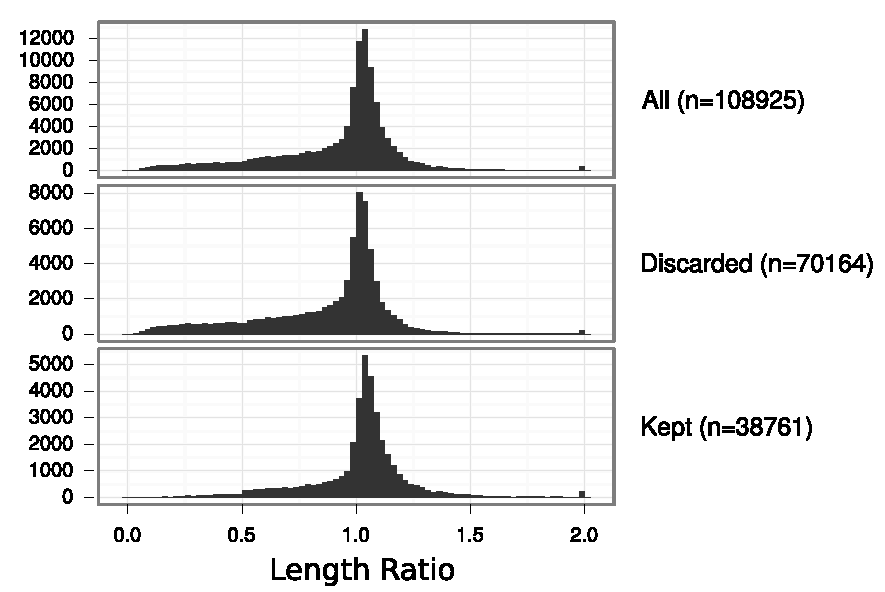
\includegraphics[scale=0.9]{Figs/mammals_paralogs_hist.pdf}
\caption{Length ratios of putative paralogs. The length ratio was
  calculated as the length of a putative paralogous copy divided by
  the mean length all sequences its corresponding gene
  tree. Putatively paralogous genes (top panel) were either discarded
  (middle panel) or kept (bottom panel) according to rules based on
  their length and mean sequence divergence from other aligned
  sequences, as described in the text.}
\label{filtered_paralogs_hist}
\end{figure}

These rules were applied to each of the 108,925 putative paralogs
within the 9,604 gene trees containing at least one set of putative
paralogs. Figure \ref{filtered_paralogs_hist} shows the distributions
of length ratios for the set of all putative paralogs, those discarded
from the alignments, and those kept for subsequent analysis. The
overall distribution of length ratios showed that most putative
paralogs had lengths similar to the mean length across the gene tree
(with a peak at or slightly above 1), but the shape of the
distribution was asymmetric, with a bias towards shorter lengths. The
filtering protocol effectively removed these shortened genes, as
evidenced by the enrichment of lower length ratios in the distribution
of discarded genes and the less skewed distribution of length ratios
in the set of 38,761 retained putative paralogs.

\begin{figure}
\centering
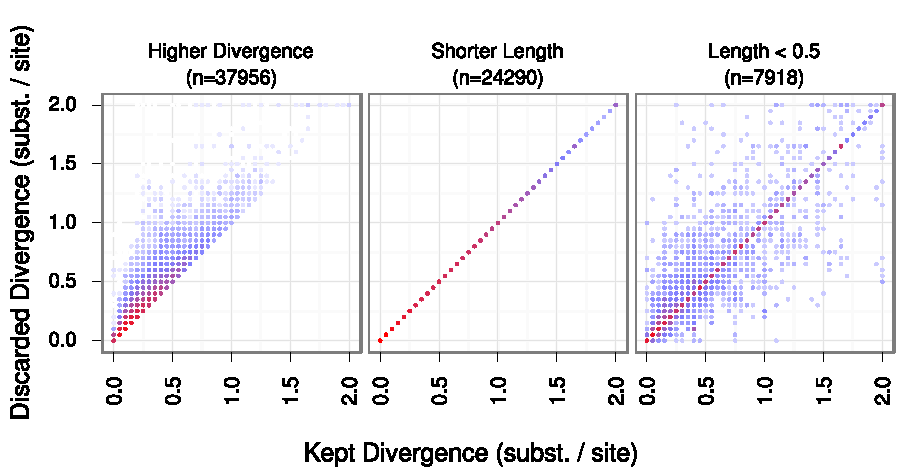
\includegraphics[scale=0.9]{Figs/mammals_paralogs_scatter.pdf}
\caption{Sequence divergence of retained and discarded putative
  paralogs. Each data point was a gene which was discarded from the
  tree for one of three reasons: it had a length ratio of less than
  0.5 while the retained copy had a length ratio greater than 0.5
  (\emph{Length $<0.5$}; right panel), it had more sequence divergence
  than the retained gene (\emph{Higher Divergence}; middle panel), or
  it had equal sequence divergence but shorter length than the
  retained gene (\emph{Shorter Length}; right panel). Divergence was
  measured as the mean pairwise divergence between the gene and all
  other sequences in the tree. Each colored point represents the
  binned density of sites; no points are drawn where no density
  exists, while blue and red points are drawn at areas of low and high
  density, respectively.}
\label{filtered_paralogs_scatter}
\end{figure}

A more detailed view of the results of the paralog filter is presented
in Figure \ref{filtered_paralogs_scatter}, showing a scatter plot of
the mean distance and length ratio of each discarded paralog compared
to that of the corresponding kept paralog. Figure
\ref{filtered_paralogs_scatter} is separated into panels according to
the rule used to discard the paralogous copy: the first panel
corresponds to rule (1), where genes with a length ratio below 0.5
were discarded; the second panel corresponds to rule (2), where genes
with higher mean distances were removed; the third panel corresponds
to rule (3), where all genes had equal mean distances and the longest
gene was kept (or, if all lengths were equal, an arbitrary choice was
made).

The first panel of Figure \ref{filtered_paralogs_scatter} shows that
genes discarded on the basis of having a very short length contained
sequence distances similar to the kept copies, as the highest density
is along the diagonal and there is perhaps only a slight bias towards
genes lying above the diagonal (i.e., in the direction of greater
divergence in the discarded copy). This was in line with the
expectation that these discarded genes were not truly paralogous
copies, but rather fragments of split genes resulting from unassembled
sequence segments. The second panel shows that when paralogous copies
could be differentiated by their mean distances, they tended to have
low average distances ($<$0.5 substitutions per nucleotide site) and
only a small difference between the kept and discarded copy (e.g.,
most of the distribution is just above the diagonal, and few points
are above the dashed line with a slope of 2). Finally, the
distribution of length ratios and mean distances in the set of genes
where length was the discriminating factor (or where an arbitrary
decision was made) shows that most of these genes were mostly
identical whether measured by sequence distance or by sequence length.

These results provided evidence that a sizeable fraction of recently
duplicated mammalian genes are identical or very similar to each
other: for roughly 30\% of all putative paralogs, not enough time has
elapsed since the duplication event for a detectable amount of
sequence change to have occurred, and the choice between retaining one
copy or the other was essentially arbitrary. For the roughly 40\% of
putative paralogs where differences in mean distance could be
identified, these differences tended to be small.

This was obviously not the most conservative approach to dealing with
recent duplications. One could instead remove all putatively
paralogous copies from the gene tree, creating an apparent gene
deletion in that species, or simply ignore all gene families with any
recent duplications (e.g., require one-to-one orthology allowing for
gene deletions). The latter option would likely be overly restrictive
for any sensible genome-wide analysis, but the former option may be
appropriate for a more conservative approach. As the main concern over
the handling duplicated genes has been that they may introduce a bias
towards elevated evolutionary rates, I marked the genes containing
sets of putative paralogs for further evaluation. Sitewise estimates
from these genes were excluded from the most conservatively-filtered
sitewise dataset and examined separately for excess signal of positive
selection (see Section \ref{section_sitewise_filtering})
%, and in the
%next chapter I examine whether using the more conservative approach of
%removing all paralogous copies from genes removed the signal of
%positive selection from a subset of genes (see Section
%\ref{section_genes_paralog_subset}).

\subsection{Identifying clusters of \nsyn substitutions}
\label{section_windows_clustered_subs}

After filtering for sequence quality and removing paralogous genes and
shortened gene fragments, \prankc was used to align the codon
sequences of each of the \ntrees mammalian gene trees. Manual analysis
of a number of these alignments revealed many short stretches of
clearly nonhomologous sequence in one species, often flanked by
stretches of perfect homology and often lying on the borders of exon
junctions. Examples of two such regions are shown in Figure
\ref{fig_mammals_cluster_subs}.  These obviously erroneous stretches
were likely due to mis-assembly of a genomic region or
misidentification of exon boundaries within the gene of one
species. In the examples in Figure \ref{fig_mammals_cluster_subs},
most of the nonhomologous material was inferred to be a
lineage-specific insertion in the mis-annotated species; these regions
were not of concern, as \ac{slr} ignores single-species insertions
because they contain no evolutionary information. More concerning,
however, were the regions indicated with red brackets in Figure
\ref{fig_mammals_cluster_subs} where the apparently \nhom material was
aligned with other species. These regions were particularly concerning
with respect to the detection of positive selection, as the
incorporation of a stretch of apparently nonhomologous material into a
sequence alignment would produce many alignment columns with multiple
nucleotide differences per codon. As discussed in Section
\ref{sec_error_impact}, this type of error is particularly prone to
cause false positives in the detection of positive selection.

\begin{figure}
\centering 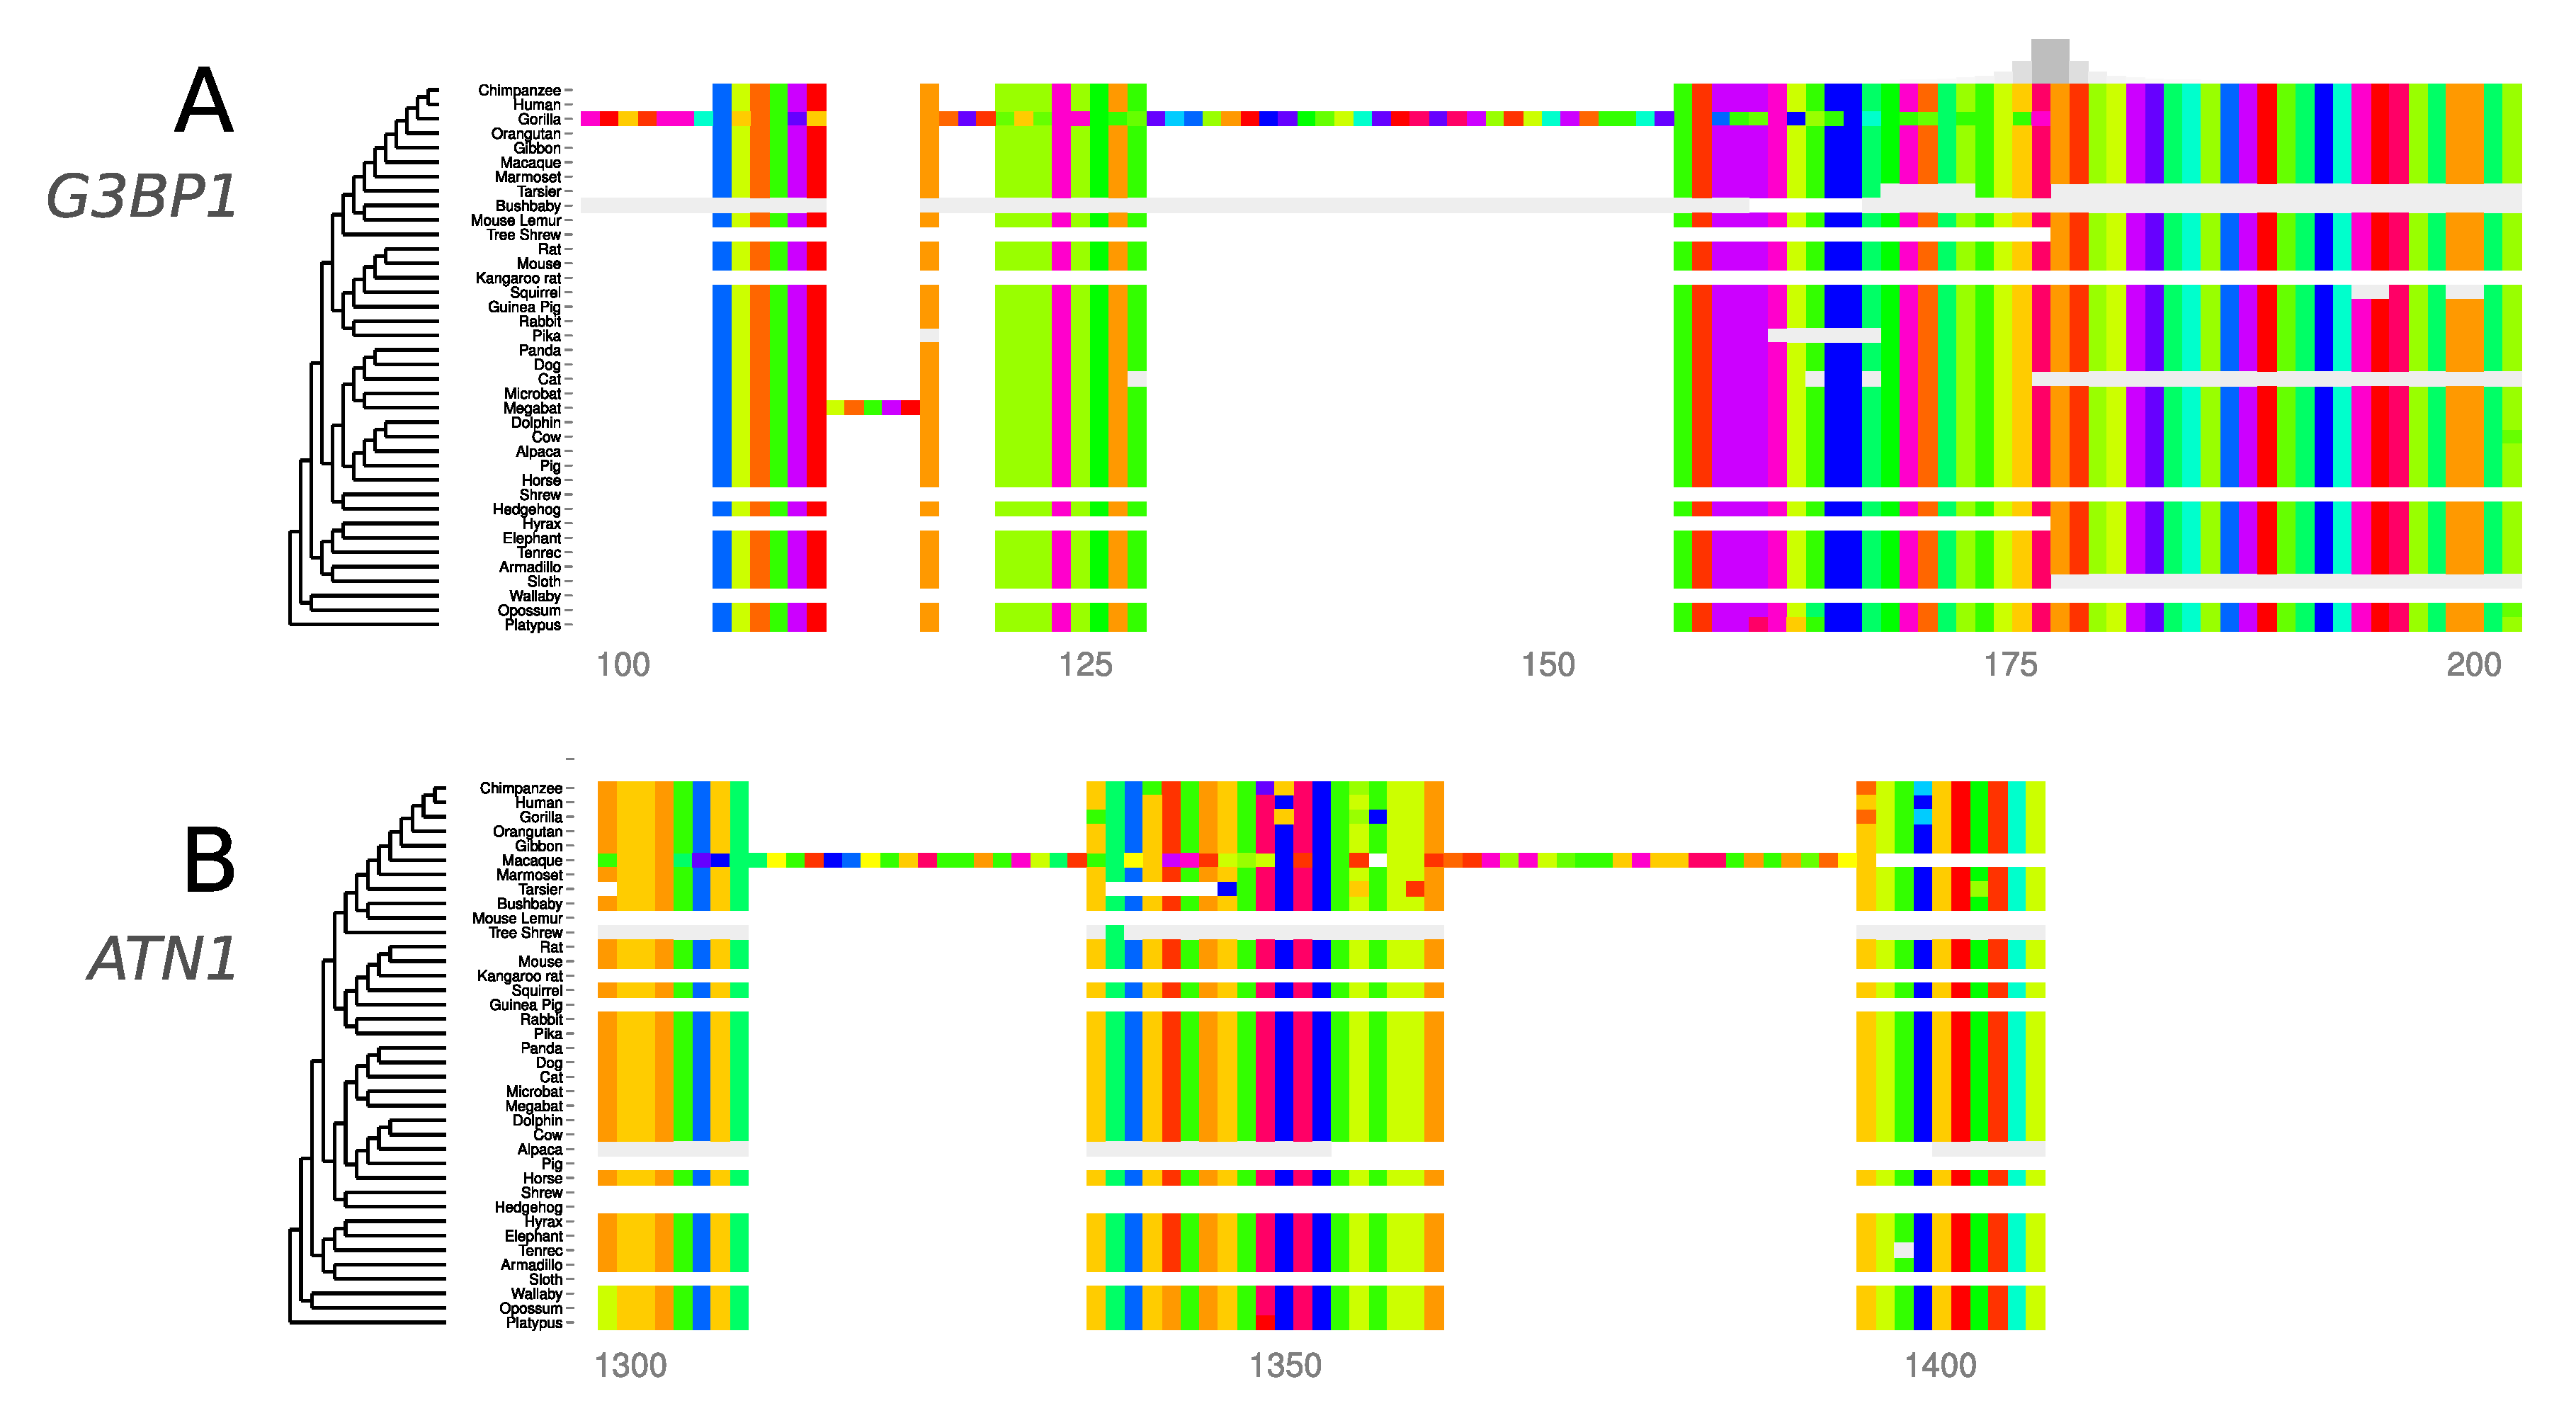
\includegraphics[scale=0.25]{Figs/mammals_cluster_subs.pdf}
\caption{Two regions of protein-coding mammalian alignments with
  stretches of \nhom sequence in one species. Alignments are shown
  with amino acids colored according to \citet{Taylor1986}. (A) The
  \gene{G3BP1} alignment, showing a mis-annotated exon in gorilla
  resulting in misalignment. (B) The \gene{ATN1} alignment, showing a
  mis-annotated exon in macaque resulting in misalignment. The regions
  indicated by red brackets contained aligned \nhom material that
  might cause false positives in detecting \sw positive selection.}
\label{fig_mammals_cluster_subs}
\end{figure}

I hypothesized that these stretches of \nhom sequence could be
identified by their impact on the pattern of substitutions within each
alignment. A stretch of \nhom aligned sequence would be expected to
produce a localized cluster of apparent synonymous and nonsynonymous
substitutions occurring along the branch between the sequence
containing the erroneous stretch and its ancestor. Because these
substitutions would be restricted to one terminal branch in the gene
tree and a region of the alignment limited to the length of the \nhom
stretch, a scan for clustered substitutions within the terminal
lineages of genes might be an effective way of identifying these
erroneous sequences.

Two factors could confound the effectiveness of using clustered
substitutions to identify regions of \nhom aligned sequence. First,
the length of the terminal branch leading to each species determines
how many lineage-specific substitutions would be expected to occur
within a window of a certain size. The terminal human branch, for
example, is very short, while the platypus branch is very long. Thus,
one would expect to observe many more lineage-specific substitutions
in platypus than in human for a given alignment window. In contrast, a
stretch of \nhom aligned sequence should introduce, on average, a
constant number of \nsyn and \syn substitutions into the branch
ancestral to the sequence in which it exists. For this reason it
should be more difficult to distinguish homologous from \nhom
stretches in species with long terminal lineages. On the other hand,
this trend should also serve to limit the negative impact of \nhom
stretches in those species on the detection of positive selection,
because the resulting elevation in \nsyn or \syn substitutions rates
would be less severe.

The second confounding factor is that \nsyn substitutions have been
shown to be significantly more clustered than expected by chance in a
number of genomic analyses of mammalian and insect genomes
\citep{Callahan2011,Bazykin2004,Wang2007}. Thus, a filter based on
clustered \nsyn substitutions may have a tendency to remove true
clusters of \nsyn substitutions from the dataset. The influence of
this factor may be evaluated by comparing clusters of substitutions in
terminal branches to those in internal branches: while both internal
and terminal branches of the mammalian tree should harbor similar
levels of truly clustered \nsyn and \syn substitutions, only the
terminal lineages should contain large clusters resulting from
stretches of aligned \nhom sequence.

I investigated the distributions of \nsyn and \syn substitutions
within windows of mammalian alignments by using \emph{codeml}
\citep{Yang2007PAML} under the M0 model (e.g., assuming one \omg for
all sites and all branches in the tree) to perform the marginal
reconstruction of ancestral sequences at internal nodes
\citep{Yang1995} and to identify the substitution events implied by
the reconstructed ancestral sequences of each gene alignment. Only
substitution events occurring between codons with high posterior
probabilities in the marginal ancestral reconstruction ($>0.9$) were
analyzed, and the location of each substitution event along the
alignment and within the gene tree was stored. This analysis was
performed on all gene trees, yielding a large database of confidently
inferred substitution events along internal and terminal branches of
the mammalian phylogenetic tree.

Counts of \syn and \nsyn substitutions along each branch were
separately collected for non-overlapping 15-codon alignment windows;
the results for a selection of species and internal nodes are shown in
Figure \ref{fig_wcs}, which plots the number of 15-codon windows
containing a given number of \nsyn and \syn substitutions for a
selection of terminal and internal nodes. Each window is thus
represented twice in Figure \ref{fig_wcs}: once in the \nsyn
histogram, and once in the \syn histogram. Windows with no
substitutions along the given branch are represented in the left-most
\syn and \nsyn bins. The mean length of the branch ancestral to the
given node, calculated from the set of branch lengths estimated by
\emph{codeml}, is indicated in parentheses after each node name.

\begin{figure}
\centering 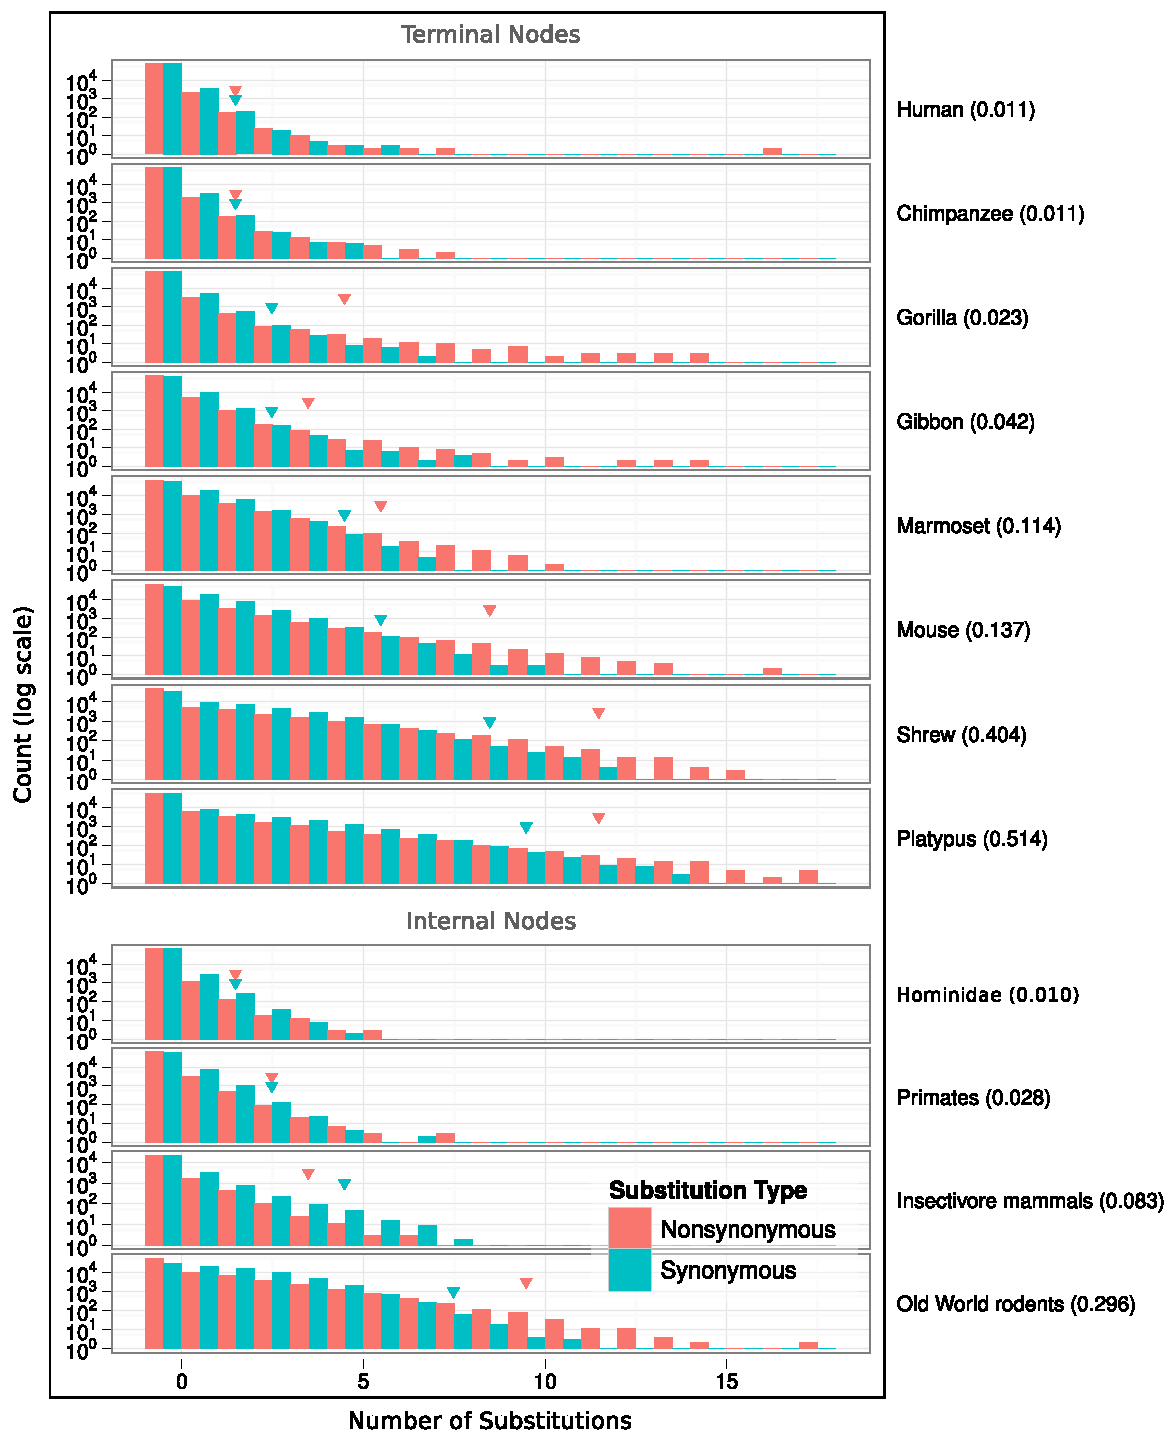
\includegraphics[scale=0.75]{Figs/wcs_15.pdf}
\caption{Counts of inferred \nsyn (red bars) and \syn (blue bars)
  substitutions in 15-codon windows along terminal and internal
  branches of the mammalian tree. The leftmost two bars correspond to
  windows with 0 substitutions, the next two bars correspond to
  windows with 1 substitution, and so on. Red and blue arrows indicate
  the number of \nsyn and \syn substitutions, respectively,
  corresponding to the 99.9\% percentile across all windows in that
  node. The mean length of the branch ancestral to each node is
  included in parentheses after the node label.}
\label{fig_wcs}
\end{figure}

Figure \ref{fig_wcs} shows that the vast majority of 15-codon windows
in these alignments contained few substitutions (note that the
$y$-axis uses a logarithmic scale), but a long tail of \nsyn and \syn
substitutions were observed for some nodes. Comparing the counts of
\nsyn vs.\ \syn substitutions within the terminal nodes (Figure
\ref{fig_wcs}, top panel), a pattern is seen where the \nsyn counts
(red bars) are higher than \syn counts at 0 substitutions, lower than
\syn counts in the middle range of substitutions (1--5 substitutions),
and higher again in the higher range of substitutions ($>$5
substitutions). The pattern in the lower range is consistent with the
action of purifying selection on protein-coding regions, causing a
reduced number of windows with multiple \nsyn substitutions compared
to \syn substitutions. The excess of windows with large numbers of
\nsyn substitutions, on the other hand, runs against the pattern of
purifying selection; instead, it shows unexpectedly long clusters of
\nsyn substitutions to be a widespread feature of these mammalian
alignments. The red and blue triangles drawn in each plot mark the
number of substitutions below which 99.9\% of windows are contained;
the shift of the \nsyn markers to the right in most of the terminal
branches emphasizes the excess of highly clustered \nsyn
substitutions. Interestingly, human---which has the highest quality
and best annotated genome---does not show the same level of excess
seen in the other genomes analyzed.

Comparing the pattern seen for terminal nodes to those from internal
nodes provided further evidence for the presence of many stretches of
\nhom sequence within the mammalian alignments. For example, the
terminal gorilla node is roughly equivalent in average branch length
to the internal primates node ($0.023$ vs.\ $0.028$), but gorilla
contains windows with up to 14 \nsyn substitutions while primates
contain a maximum of 8. Looking at the \nsyn and \syn 99.9\%
quantiles, three of the four internal nodes had equal or lower
quantile positions for \nsyn versus \syn substitutions, but the rodent
ancestral node showed a pattern more similar to the terminal nodes in
Figure \ref{fig_wcs}, with a higher 99\% quantile for \nsyn
substitutions. This was an interesting difference, as the gene
annotations for most rodent genomes were likely derived from
alignments to mouse rather than human. In the case of discordant gene
annotations, the entire rodent clade would share an aligned \nhom
stretch, causing clustered substitutions to be inferred along the
internal rodent branch. This raised the possibility that the entire
rodent clade contains many misaligned \nhom stretches due to shared
differences in gene annotations between rodent and non-rodent species.

%This appeared to be the case for at least one gene: Figure
%\ref{fig_mouse_crap_aln} shows the region surrounding a 15-codon
%window with 11 apparent rodent \nsyn substitutions, likely the result
%of a difference in exon annotations between rodent and non-rodent
%genomes.

The end result of this analysis was the identification, for each
terminal node of the mammalian tree, of windows with \nsyn
substitution counts above the top 0.1\% of 15-codon windows; these
windows were considered potential stretches of \nhom aligned
sequence. Despite evidence that some internal nodes might also suffer
from this type of alignment artifact, most internal nodes were free
from an obvious excess of clustered \nsyn substitutions, so internal
nodes were excluded from this list. A qualitative analysis of regions
containing windows at a variety of thresholds found the 0.1\%
threshold to strike a good balance between sensitivity and
specificity.

In total, 37,824 windows containing potential stretches of \nhom
aligned sequence were identified across 8,951 alignments, with 881
genes containing more than 10 windows each. The locations of these
windows were stored for later use in defining the most
conservatively-filtered sitewise dataset.

%\section{Genome-wide analysis of sitewise selective pressures in mammals}

\section{Species groups for sitewise analysis}

% latex table generated in R 2.13.0 by xtable 1.5-6 package
% Thu Sep 15 11:19:59 2011
\begin{table}
\centering \footnotesize
\begin{tabular}{lrb{8cm}rr}
\toprule
 & \multicolumn{2}{c}{Species} & \multicolumn{2}{c}{Median dS} \\
\cmidrule(r){2-3} \cmidrule{4-5}
Name & Count & List & MPL & Total \\
  \midrule
\input{Tables/table_species_set_summary.txt}
\bottomrule
\end{tabular}
\caption{Species groups used for sitewise analysis by \ac{slr}. The
  median \acp{mpl} and the median total branch length are shown for
  each species group, taken from the \ntrees branch lengths estimated
  by \ac{slr} for each gene. MPL -- mean path length.}
\label{table_species_set_summary}
\end{table}

For each alignment of mammalian orthologs, SLR was run separately on
10 different sets of mammalian species to obtain sitewise estimates in
a variety of species groups. For each species group, sequences
corresponding to species within the group were extracted from the
whole mammalian alignment (along with the corresponding \subtr) and
input to SLR, which was run with its default parameters. If fewer than
two sequences were available for a given gene and species group, the
sitewise analysis was skipped for that group. The species included in
each group are listed in Table \ref{table_species_set_summary}
alongside the \acf{mpl} and total branch length of their subtrees,
estimated as the median value across all \ntrees genes' estimates of
\ds distances.

Three of the species groups (Glires, Primates, and Laurasiatheria) were
chosen because they represent the three mammalian superorders with the
greatest taxonomic representation in Ensembl, providing an opportunity
to compare the molecular evolutionary dynamics of three monophyletic
mammalian groups containing varying levels of divergence, diverse
biological characteristics, and a number of high-quality reference
genomes. A fourth parallel mammalian subclade, Atlantogenata,
consisting of sloth, armadillo, tenrec, elephant and hyrax, was also
included, but the monophyly of this group is still under debate
\citep{Murphy2007,Churakov2009} and it contains only one high-coverage
genome. As such, it was not considered a primary target for the
mammalian superorder analysis. The different mammalian superorders
contained a wide range of total branch lengths, with 0.83 for
Primates, 0.97 for Atlantogenata, 1.90 for Glires, and 2.16 for
Laurasiatheria. A slightly different ordering was found when measuring
the trees by \ac{mpl}, with Glires having a significantly higher
\ac{mpl} (0.40) than the other groups despite having fewer species and
a lower total branch length than Laurasiatheria. This reflected the
higher neutral evolutionary rate in the Glires group, a
well-documented feature of rodent evolution likely resulting from
their long-term shorter generation time, which has been strongly
correlated with higher neutral evolutionary rates
\citep{Nikolaev2007,Smith2008}.

Two larger species groups, Eutheria and Mammalia, were chosen for the
purpose of measuring average sitewise selective pressures across
mammals as a whole. The Eutheria group consists of the union of the
mammalian superorder groups plus armadillo, and the Mammalian group
adds opossum, platypus, and wallaby for a total of 38 species. The
median total branch lengths for Mammalia and Eutheria were 8.21 and
6.43, respectively, and the \ac{mpl}s were 0.67 and 0.35.

Finally, to evaluate the impact of species choice and branch length on
the results of the \sw analysis, four additional ``sparse'' species
groups were created for comparison to the main groups of interest. The
species in the Sparse Glires group were chosen to create a group with
species from the Glires group but having a lower overall branch
length; the Sparse Mammals group was created with a similar aim,
created by selecting one species (preferably with a high-coverage
genome) from each major mammalian branch, greatly reducing the total
branch length covered but maintaining a similar evolutionary depth and
distribution of major branches within the species tree. The HQ Mammals
group was similar to the Sparse Mammals group, but elephant and the
deeper mammalian lineages were omitted (i.e., wallaby, platypus,
armadillo) in favor of only the high-coverage Eutherian genomes (i.e.,
chimpanzee, cow, horse, macaque, pig, rat). Finally, the HMRD group
consisted of human, mouse, rat, dog, and represented the type of
phylogenetic tree that was commonly analyzed early in the last decade
when only a few mammalian genome sequences were available. The HMRD
group was comparable to Primates and Atlantogenata in total branch
length, while HQ Mammals and Sparse Glires were more similar to
Glires.

\section{Evaluating and filtering \sw results}
\label{section_sitewise_filtering}

Sitewise data were collected from SLR and stored in a database for
storage and further analysis. The Mammals group, containing the
greatest total branch length of all the datasets and representing the
entire set of aligned sequences, and the Primates group, containing
the lowest overall branch length, were used as representative species
groups to perform quality-control checks on the \sw data and to guide
the curation of filtered \sw datasets for each species group.

Two genome-wide datasets were generated by processing \sw data
separately with two levels of filtering: a relaxed filter, designed to
retain much of the data while filtering out the most obviously
low-quality sites, and a conservative filter, designed to remove a
wider set of sites and genes that showed evidence for potential
misalignment or large numbers of gene duplications.

\bbfig
\centering
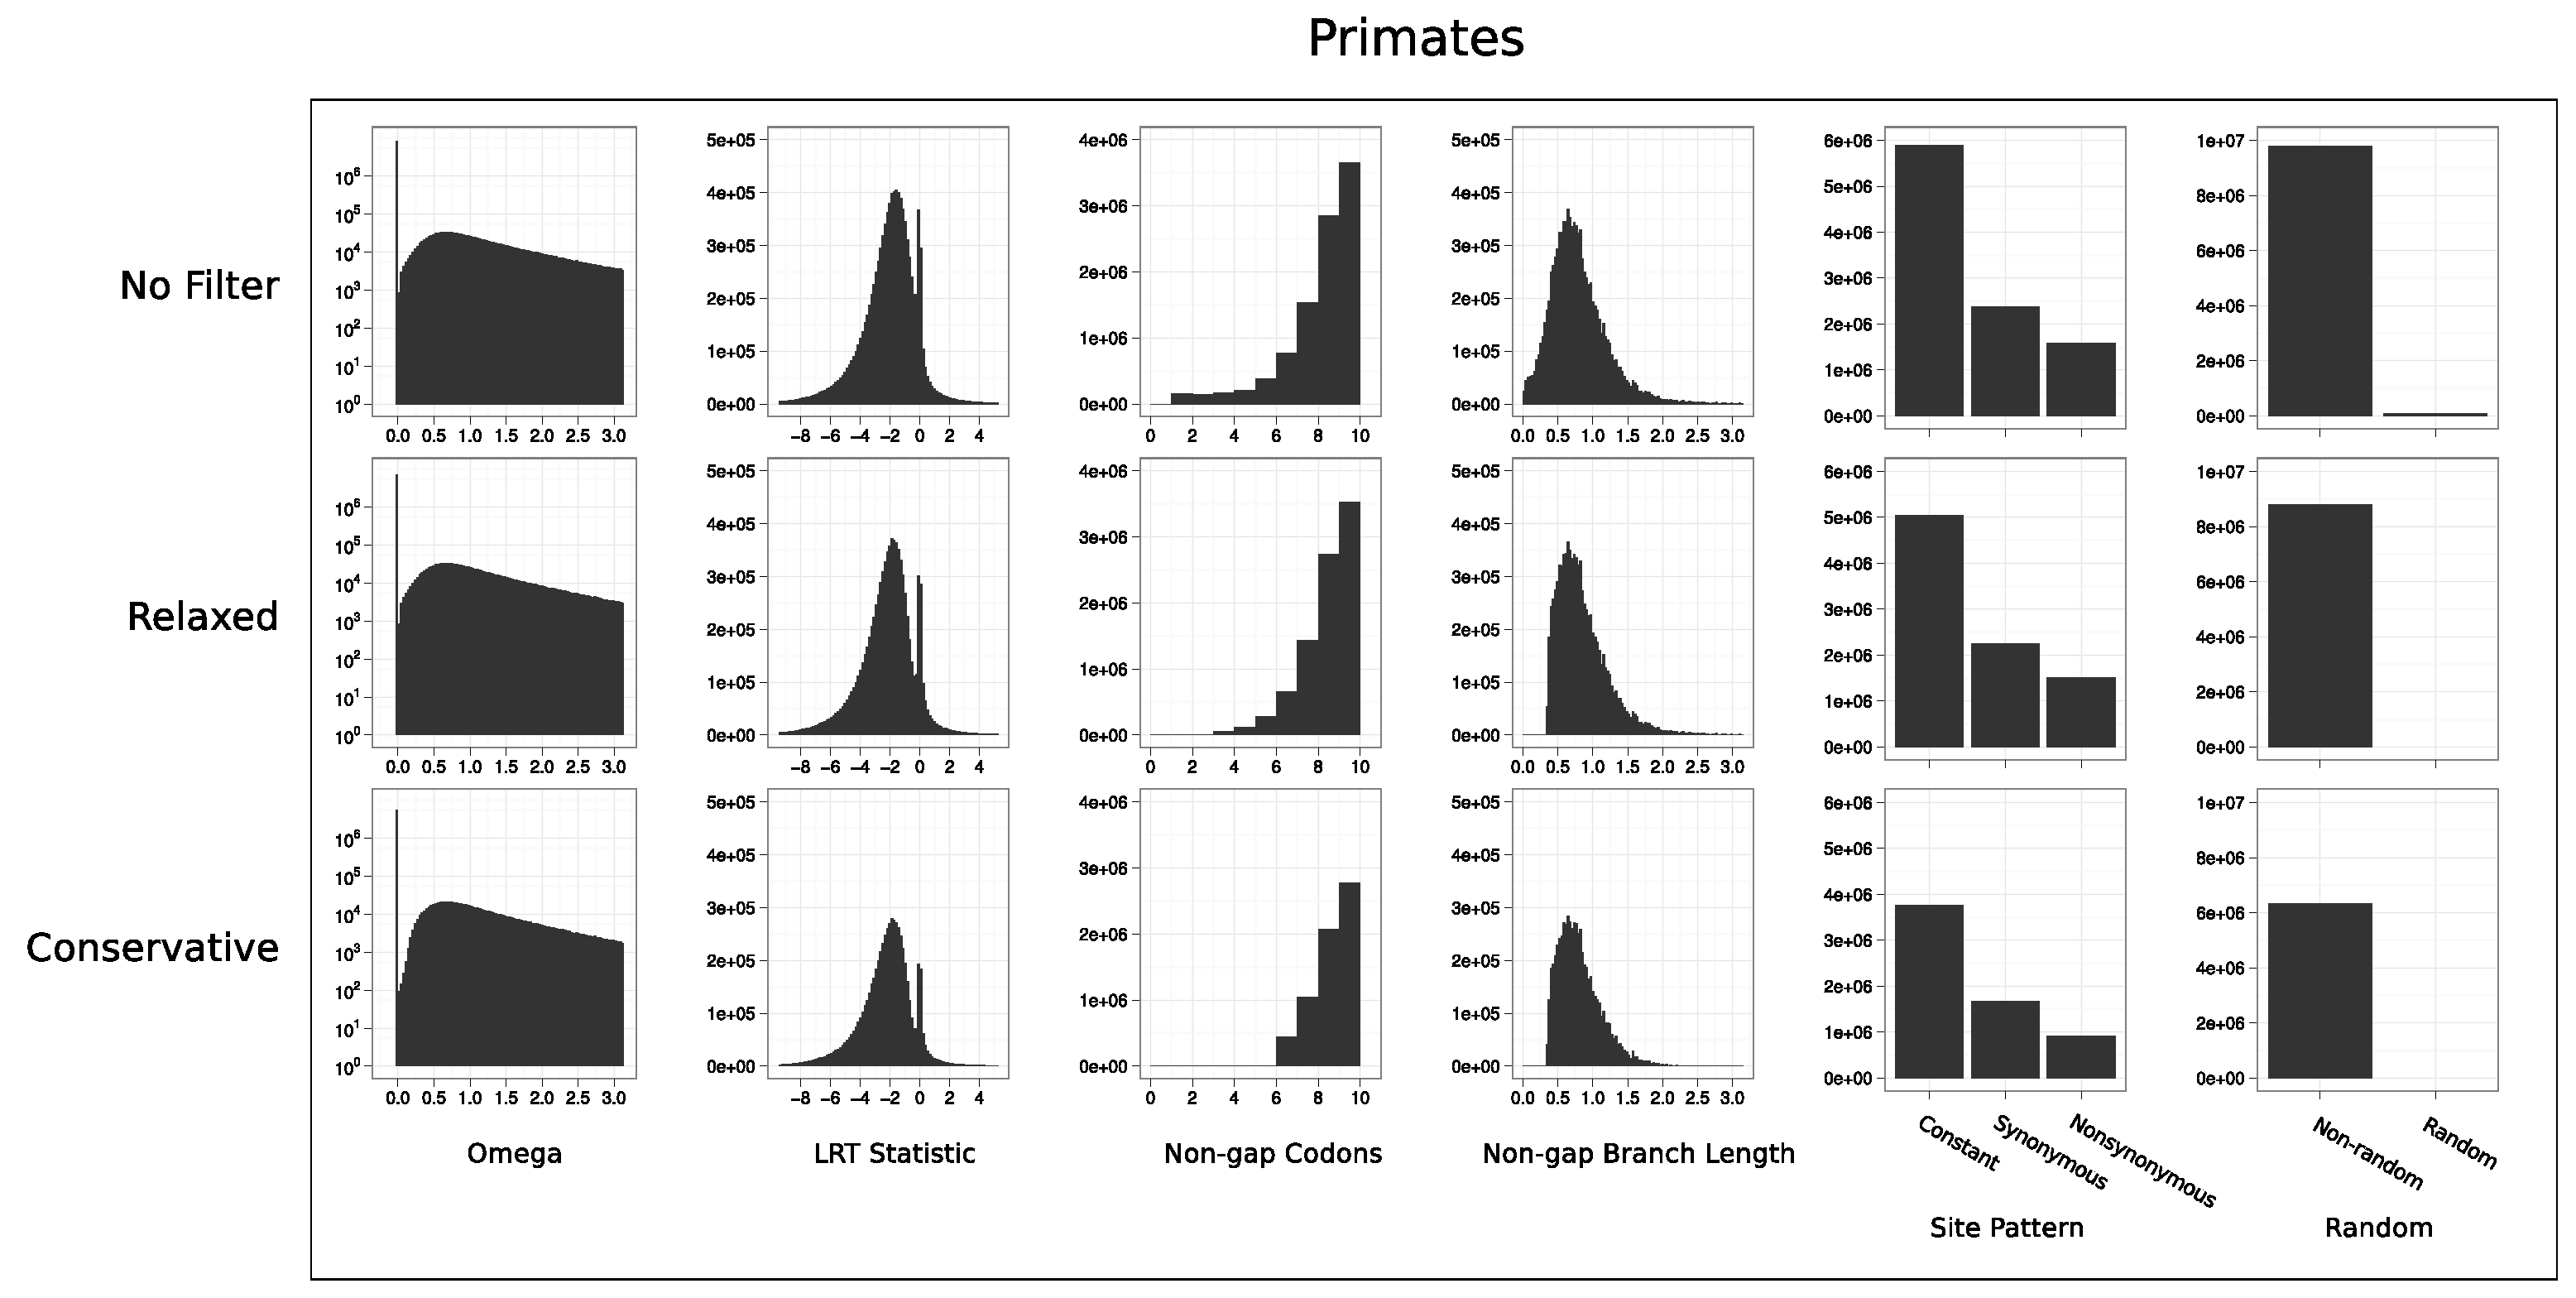
\includegraphics[scale=0.42]{Figs/qc_hist_primates.pdf}
\caption{Distributions of sitewise values for the Primates species
  group, showing the raw data (top row) and the result of applying the
  relaxed (middle row) and conservative (bottom row) filters.}
\label{fig_qc_hist_primates}
\eefig

\bbfig
\centering
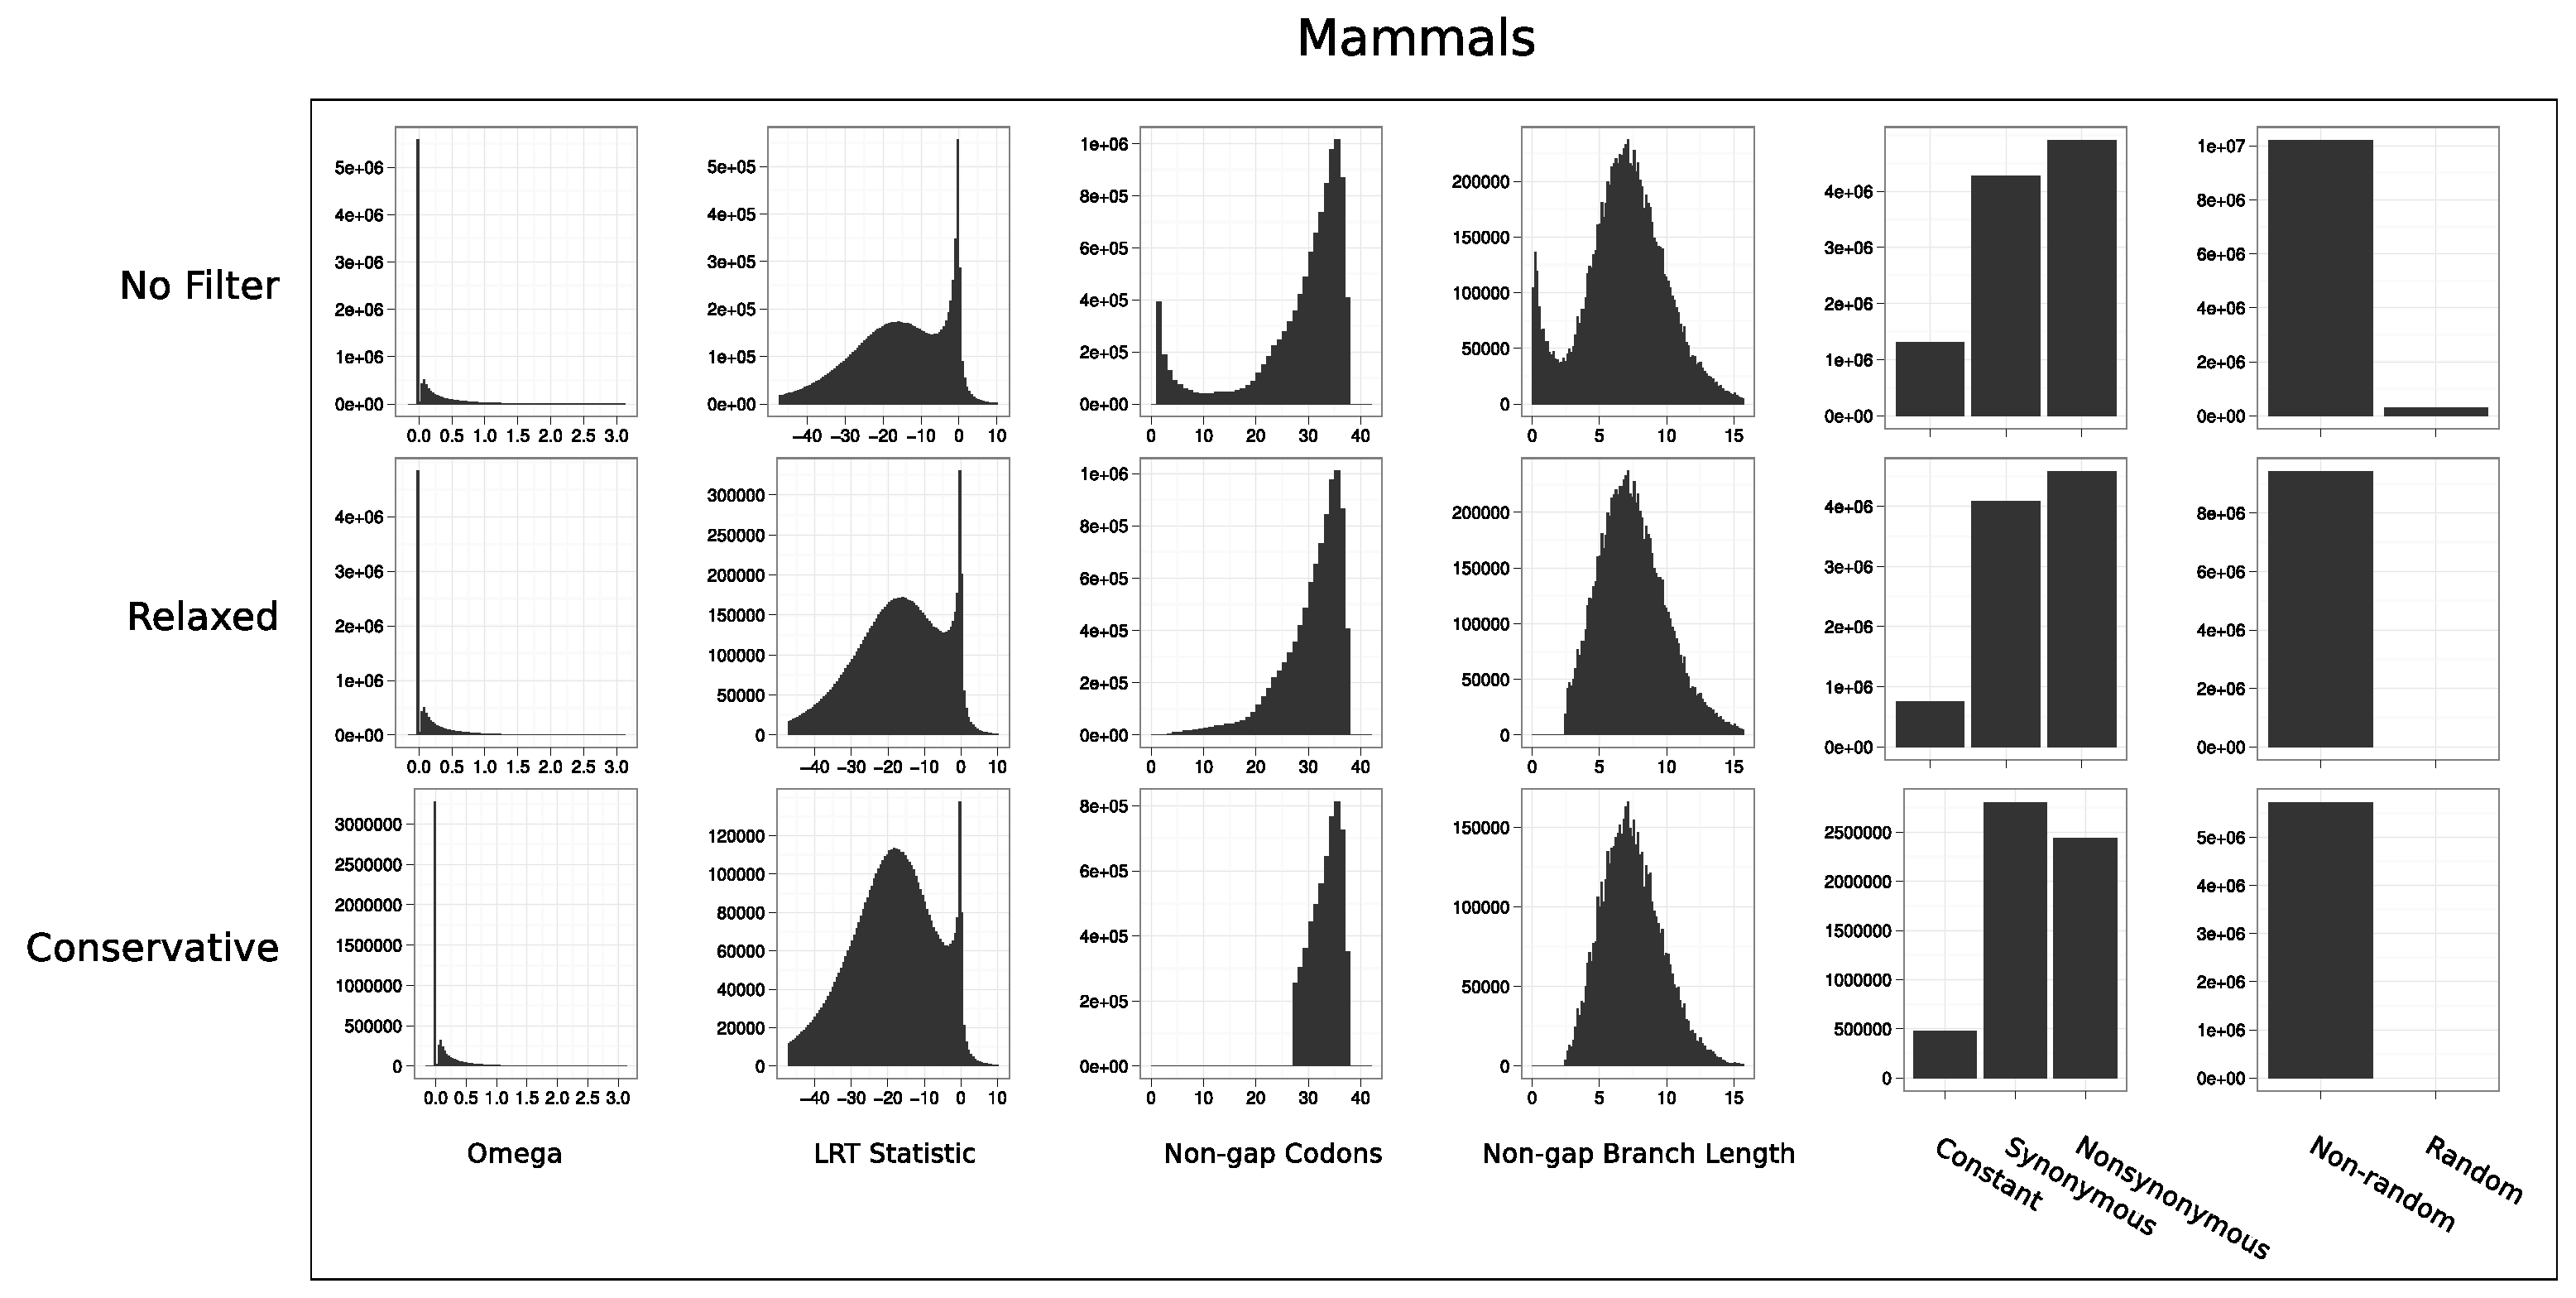
\includegraphics[scale=0.42]{Figs/qc_hist_mammals.pdf}
\caption{Distributions of sitewise values for the Mammals species
  group, showing the raw data (top row) and the result of applying the
  relaxed (middle row) and conservative (bottom row) filters.}
\label{fig_qc_hist_mammals}
\eefig
 
I first examined the overall distributions of \omg estimates and \sw
LRT statistics from SLR. Figures \ref{fig_qc_hist_primates} and
\ref{fig_qc_hist_mammals} show the distributions of six sitewise
statistics for each group of species. Four of the statistics (Omega,
LRT Statistic, Site Pattern and Random) were collected from the output
of \ac{slr} and two of the statistics (\Ngap Codons and \Ngap Branch
Length) were directly calculated from the codon alignments. The Omega
statistic is \ac{slr}'s \ac{ml} estimate of \omg, hereafter referred
to as \omgml. The LRT Statistic is the raw statistic resulting from
the \sw \ac{lrt} performed by \ac{slr}. Following Massingham
\citeyearpar{Massingham2005}, a signed version of the \ac{lrt}
statistic, hereafter \slrt, is used throughout this chapter. The \slrt
is formed by negating the raw \ac{lrt} statistic for sites where
\omgml$<1$; the signed statistic is a useful measure by which to sort
sites according to their evidence for purifying and positive
selection. The Site Pattern is a categorical classification of the
pattern of \syn and \nsyn substitutions at each site: a site is
``constant'' if it contains no differences, ``synonymous'' if it only
contains \syn differences between sequences, and \nsyn if it contains
at least one \nsyn difference. Sites designated as ``Random'' contain
a pattern of codons not significantly different from random, as
calculated by \ac{slr} based on the entropy and optimized likelihood
at that site. Finally, the \Ngap Codons and \Ngap Branch Length
statistics were calculated from the pattern of gaps and non-gaps at
each alignment column: \Ngap Codons is a count of the number of
sequences without gaps at that site, and \Ngap Branch Length measures
the total branch length of the \subtr connecting each of the \ngap
sequences.

A prominent feature of the distribution of \omgml values for the
unfiltered Mammals data, shown in the top row of Figure
\ref{fig_qc_hist_mammals}, was the large number of sites with
\omgml$=0$. Further inspection of the data revealed that all
\omgml$=0$ sites contained either \syn or constant site patterns. In
fact, all sites with constant patterns (and nearly all sites with \syn
patterns) yielded a \omgml estimate of zero. Intuitively, an estimate
of zero for \syn sites is appropriate, as the lack of any \nsyn
substitutions throughout the tree would provide no evidence for a
\nsyn substitution rate of greater than zero. For constant sites the
case is less clear, because no data regarding the rate of either \syn
or \nsyn substitutions exists in the alignment column. However, given
SLR's assumption of a constant \syn substitution rate throughout each
gene \citep{Massingham2005}, the \omg value which maximizes the
likelihood of observing zero substitutions is zero, since that value
minimizes both the \nsyn and the total substitution rate.

It is not evident from either Figure \ref{fig_qc_hist_primates} or
\ref{fig_qc_hist_mammals}, but a small proportion (ca. 0.2\%) of sites
containing \syn site patterns resulted in \omgml estimates greater
than zero. Analysis of the alignment columns corresponding to these
sites showed them all to include synonymous codons coding for serine
or arginine which are separated by multiple nucleotide
differences. Under the mechanistic codon model implemented by
\ac{slr}, which does not allow for multiple simultaneous nucleotide
changes, inferring an evolutionary path between these
multiply-substituted codons required the inference of multiple \nsyn
substitutions to reach one codon from the other. This produced a \nsyn
substitution rate of greater than zero for a site with a \syn site
pattern. The existence of multiply-substituted codons in alignments
has been previously reported \citep{Averof2000,Whelan2004}, and
empirical results have supported the notion that codon models that
allow for multiple simultaneous nucleotide changes better describe
evolution than those that do not \citep{Kosiol2007}. However, the very
low proportion of synonymous sites requiring non-zero \nsyn
substitution rates suggested that the impact of these effects on the
current dataset was minimal; this was likely due to the relatively
short branch lengths separating the nodes of the mammalian tree,
making it less probable that codons differing by multiple
substitutions (whether the result of simultaneous multiple nucleotide
changes or successive single changes) would be observed
\citep{Kosiol2007}.

The distributions of the \Ngap Codons and \Ngap Branch Length values
in the unfiltered row of Figure \ref{fig_qc_hist_mammals} showed that
most alignment columns contained sequence data from many species (with
\Ngap Codons peaking at 36 and \Ngap Branch Length peaking at around 8
substitutions per site), but a noticeable portion of sites contained
only a few non-gap sequences. (For the unfiltered Primates histograms
in Figure \ref{fig_qc_hist_primates}, there was a noticeable long tail
of low \Ngap Codons values, but no excess of low \Ngap Branch Length
value sas seen in Figure \ref{fig_qc_hist_mammals}).  If the alignment
columns with low \ngap codon counts represented accurate evolutionary
histories, then the observed excess of highly-gapped sites might be
taken as an indication that insertion events in terminal lineages or
recent ancestral lineages were prominent enough throughout mammalian
evolution to leave a noticeable signature of sites with very low
non-gap codon counts. Given the many possible sources of error in the
annotation and alignment of these sequences, however, a more likely
scenario was that sites with low codon counts and low branch lengths
came from stretches of sequence which only exist in a few species as a
result of annotation or alignment error. As a result, these sites
might be expected to show a higher probability of being \nhom and
showing spurious signals of positive selection. This would make such
sites prime candidates for filtering out prior to analysis.

\begin{table}
\centering \footnotesize
\begin{tabular}{lrrrrrrrrrr}
\toprule
 & BL & \multicolumn{3}{c}{Non-gap BL} & \multicolumn{3}{c}{Non-gap Codons} & \multicolumn{2}{c}{\omgml, \%} &  \\
\cmidrule(r){3-5} \cmidrule(r){6-8} \cmidrule(r){9-10}
 & Quantile & 25\% & 50\% & 75\% & 25\% & 50\% & 75\% & $< 1$ & $> 1$ & \psfive, \% \\
  \midrule
\input{Tables/bl_pos_sel_breakdown.txt}
\bottomrule
\end{tabular}
\caption{Proportions of sites with evidence for purifying and positive
  selection in the Mammals and Primates datasets broken down by \ngap
  branch length. Sites were separated into 10 equally-sized bins of
  \ngap branch length and the sites within each bin were summarized by
  the $25^{th}$, $50^{th}$ and $75^{th}$ percentiles of \ngap branch
  length (BL) and \ngap codons, the percentage of sites with \omg
  estimated below or above 1, and the percentage of sites classified
  as \ac{psc} at a nominal 5\% \ac{fpr}. BL--branch length;
  PSC--positively selected codons.}
\label{table_bl_pos_sel_breakdown}
\end{table}

To test the hypothesis that sites with few \ngap sequences would be
less reliable for analysis than other sites, I split the \sw estimates
from the Mammals and Primates groups into ten equally-sized bins of
\ngap branch length. Sites within each bin were summarized by
calculating the percentage of sites with \omgml less than or greater
than 1, as well as the percentage of sites showing evidence for
positive selection at a nominal 5\% \ac{fpr}, hereafter referred to as
\acfp{psc}. The results of this analysis are presented in Table
\ref{table_bl_pos_sel_breakdown}. The lowest bin was a clear outlier
in the Mammals data, with approximately 18\% of sites having
\omgml$>1$ and 2\% of sites being \acp{psc}. The other 9 bins with
greater \ngap branch lengths showed fewer sites with \omg~$>1$ and
less evidence for positive selection; within those 9 bins, a pattern
of gradual increase in the proportion of sites with {{\omgml$>1$}} and
\acp{psc} was observed at progressively higher \ngap branch
lengths. The increase in evidence for positive selection with
increasing \ngap branch length could be explained by genes with higher
overall \dnds ratios (and presumably more \acp{psc}) having higher
branch lengths due to the increased rate of \nsyn substitution;
alternatively, longer branch lengths may lead to more statistical
power to detect positive selection. Overall, the pattern observed for
the Mammals data was consistent with the prediction that sites with
few \ngap sequences were not consistent with the general pattern of
\sw data. The reason for In terms of choosing an appropriate threshold on which to
filter, Table \ref{table_bl_pos_sel_breakdown} indicated that removing
sites with the lowest 10\% of \ngap branch length would remove most of
the apparently anomalous sites.

Table \ref{table_bl_pos_sel_breakdown} shows a similar trend for the
Primates dataset, although the distinction between the lowest bin and
the rest of the dataset was less obvious. The percentage of \acp{psc}
in the lowest decile was only slightly higher than in the next-highest
decile, and the proportion of sites with \omgml$>1$ was lower than in
all other bins. Thus, despite weaker evidence in the Primates data for
the anomalous nature of sites with few \ngap sequences, it still
appeared that filtering sites in the bottom 10\% bin would improve the
overall quality and consistency of the data.

Turning back to the bulk distributions in Figures
\ref{fig_qc_hist_mammals} and \ref{fig_qc_hist_primates}, two other
criteria were used to target sites for removal before analysis. First,
the rightmost panels of Figures \ref{fig_qc_hist_mammals} and
\ref{fig_qc_hist_primates} depict a small set of sites designated as
``random''. These sites were flagged by SLR as having a site pattern
not significantly different from random \citep{Massingham2005}, and
they were also targeted for removal before analysis of the global
distribution. Second, all sites with fewer than four \ngap sequences
were removed. This was done to avoid analyzing sites with very few
sequences which were not within the bottom 10\% of sites by \ngap
branchlength.

At this point, all of the criteria used to define the relaxed filter
have been described: \ngap branch lengths, the ``random'' flag, and
the number of \ngap sequences at each site.
%Table
%\ref{table_filtering_summary} summarizes the filtering criteria used,
%and 
The middle rows of Figures \ref{fig_qc_hist_primates} and
\ref{fig_qc_hist_mammals} show the summary distributions resulting
from applying the relaxed filter to the Mammals and Primates sitewise
data.

Three additional criteria were added to create the more conservative
filtered dataset. First, the threshold on \ngap sequence counts was
increased: all sites with a \ngap codon count below 75\% of the
maximum \ngap count for that species group were removed. Second, sites
and genes containing windows of clsutered \nsyn substitutions (as
identified in Section \ref{section_windows_clustered_subs}) were
removed: all sites overlapping the 23,116 15-codon windows with excess
\nsyn substitutions (using the 99.9\% quantile based definition of
excess substitutions from Section
\ref{section_windows_clustered_subs}) were masked out, and 819 genes
with greater than 10\% of sites covered by windows with excess \nsyn
substitutions were removed. Finally, the 3,333 genes which contained
more than two sets of putative paralogs were excluded.

As with the relaxed filter, the result of applying the conservative
filter to the Primates and Mammals datasets is shown in the bottom
rows of Figures \ref{fig_qc_hist_primates} and
\ref{fig_qc_hist_mammals}. Comparing between the distributions the
three rows of Figure \ref{fig_qc_hist_mammals}, the most prominent
effect of the two filters on the bulk distributions in was the removal
of the excess of sites with low non-gap branch lengths and non-gap
codon counts. The distributions of \omgml estimates and LRT statistics
were qualitatively unchanged, indicating that the overall
characteristics of the dataset were not significantly altered by this
filter.

Tables \ref{table_filter_summaries_1} and
\ref{table_filter_summaries_2} provide a quantitative summary of the
Mammals and Primates datasets before and after applying the two
filters. Also shown is the subset of sites overlapping with Pfam
domain annotations collected from \ens; as most Pfam domains represent
well-folded protein modules \citep{Finn2010}, the set of
Pfam-annotated sites were expected to exhibit stronger purifying
selection and be less prone to insertions or deletions and alignment
error. The rows labeled in parentheses summarize the set of sites
which were removed during the creation of the conservatively-filtered
dataset, either due to overlap with a window of clustered
substitutions (Clusters) or from being within a gene that contained
more than two recent duplications (Paralogs).

The columns in Table \ref{table_filter_summaries_1} show various
summary statistics of each \sw dataset including the number of sites,
the proportions of different site patterns, and the proportions of
purifying and positive selection based on \omgml estimates from
\ac{slr}. Table \ref{table_filter_summaries_2} provides the number and
proportion of identified \acp{psc} (columns under the heading
``Positively Selected Sites'') as well as the breakdown of sites into
purifying, neutral, and positively-selected at two different \ac{fpr}
thresholds (columns under the headings ``\chisqlt{0.1}'' and
``\chisqlt{0.05}'').

These views made clear the impact of extensive filtering on the levels
of positive and purifying selection observed in the data. The
unfiltered data from the Primates group contained 9.03\% of sites with
\omgml~$>1$ and 0.59\% of sites were \acp{psc} at a nominal 5\%
\ac{fpr}; the evidence for positive selection was reduced in the
conservatively-filtered data, showing 7.87\% sites with \omgml~$>1$
and 0.41\% \acp{psc}. An even stronger effect of filtering was seen
for the Mammals data, with \omgml~$>1$ being reduced from 5.68\% to
2.73\% between the unfiltered and conservatively-filtered datasets and
the percentage of \acp{psc} reduced from 0.72\% to 0.35\%.

The rows representing two sets of sites which were removed during the
conservative filtering process showed higher signals of positive
selection than the unfiltered data, suggesting that these two
filtering steps were at least somewhat effective in removing anomalous
or untrustworthy sites from the dataset. For sites removed due to
being within clusters of \nsyn substitutions, the enrichment for
signals of positive selection was clear: in Primates, 18.28\% of sites
yielded \omgml~$>1$ and 1.47\% of sites were \acp{psc} at a 5\%
\ac{fpr} threshold, more than three times the proportion of \acp{psc}
seen in the conservatively-filtered dataset. Sites removed as a result
of being within genes containing recent duplications showed less
enrichment for positive selection, but the proportions of \acp{psc}
and sites with \omgml~$>1$ were still above those seen in either the
relaxed or conservatively filtered datasets.

\begin{landscape}
\begin{table}
\scriptsize{
\centering
\begin{tabular}{lllrrrrrrrrrrrrr}
\toprule
 &  & &  \multicolumn{3}{c}{Site Pattern, \%} & Med. & 
  \multicolumn{3}{c}{Nongap BL} & \multicolumn{2}{c}{\omgml} &
\multicolumn{4}{c}{\omgml Below / Above, \%} \\
\cmidrule(r){4-6} \cmidrule(r){8-10} \cmidrule(r){11-12} \cmidrule(r){13-16}
Name & Filter & Sites & Const. & Syn. & Nsyn. & Codons & Med. & Mean & SD & Mean & SD &
$< 0.5$ & $< 1$ & $> 1$ & $> 1.5$ \\
  \midrule
\input{Tables/filter_summaries_1.txt}
\bottomrule
\end{tabular}
\caption{\scriptsize Summary statistics of \sw estimates for Mammals and Primates
  data with various filters applied. Rows labeled (Clusters) and
  (Paralogs) contain sites excluded by the Conservative
  filter. Columns under the ``\omgml Below / Above'' heading measure
  the percentage of sites with \omgml below or above the indicated
  value. Med.---median, Const.---constant, Syn.---\syn, Nsyn.---\nsyn,
  BL---branch length. \label{table_filter_summaries_1}
}

\hspace{.2in}

\centering
\begin{tabular}{llrrrrrrrrrrrrrrrrrrrrr}
\toprule
 & & \multicolumn{8}{c}{Positively Selected Sites (\%)} &
\multicolumn{3}{c}{\chisqlt{0.1}, \%} &
\multicolumn{3}{c}{\chisqlt{0.05}, \%} \\
\cmidrule(r){3-10} \cmidrule(r){7-10} \cmidrule(r){11-13} \cmidrule(r){14-16}
Name & Filter & 
  \multicolumn{2}{c}{\chisqlt{0.1}} & \multicolumn{2}{c}{\chisqlt{0.05}} &
  \multicolumn{2}{c}{\chisqlt{0.01}}& \multicolumn{2}{c}{\bhfdr{0.05}} &
  Neg. & Neut. & Pos. & Neg. & Neut. & Pos. \\
%\cmidrule(r){2-3} \cmidrule(r){4-5} \cmidrule(r){6-7} \cmidrule(r){8-9}
\midrule
\input{Tables/filter_summaries_2.txt}
\bottomrule
\end{tabular}
\caption{\scriptsize Proportions of sites subject to positive,
  purifying and neutral selection at various \slrt thresholds for
  Mammals and Primates data with varous filters applied. The method of
  \citet{Benjamini1995} was used to identify the \slrt threshold at
  which FDR$<$0.05. For columns under the headings ``\chisqlt{0.1},
  \%'' and ``\chisqlt{0.05}, \%'', Pos. and Neg. are the percentage of
  sites with significant evidence for positive and negative selection,
  respectively, and Neut. is the percentage of ``neutral'' sites not
  showing significant evidence for non-neutral selection.}
\label{table_filter_summaries_2}
}
\end{table}
\end{landscape}

\section[The global distribution of \sw selective pressures in mammals]{The global distribution of \sw selective \\ pressures in mammals}

\begin{figure}
\centering 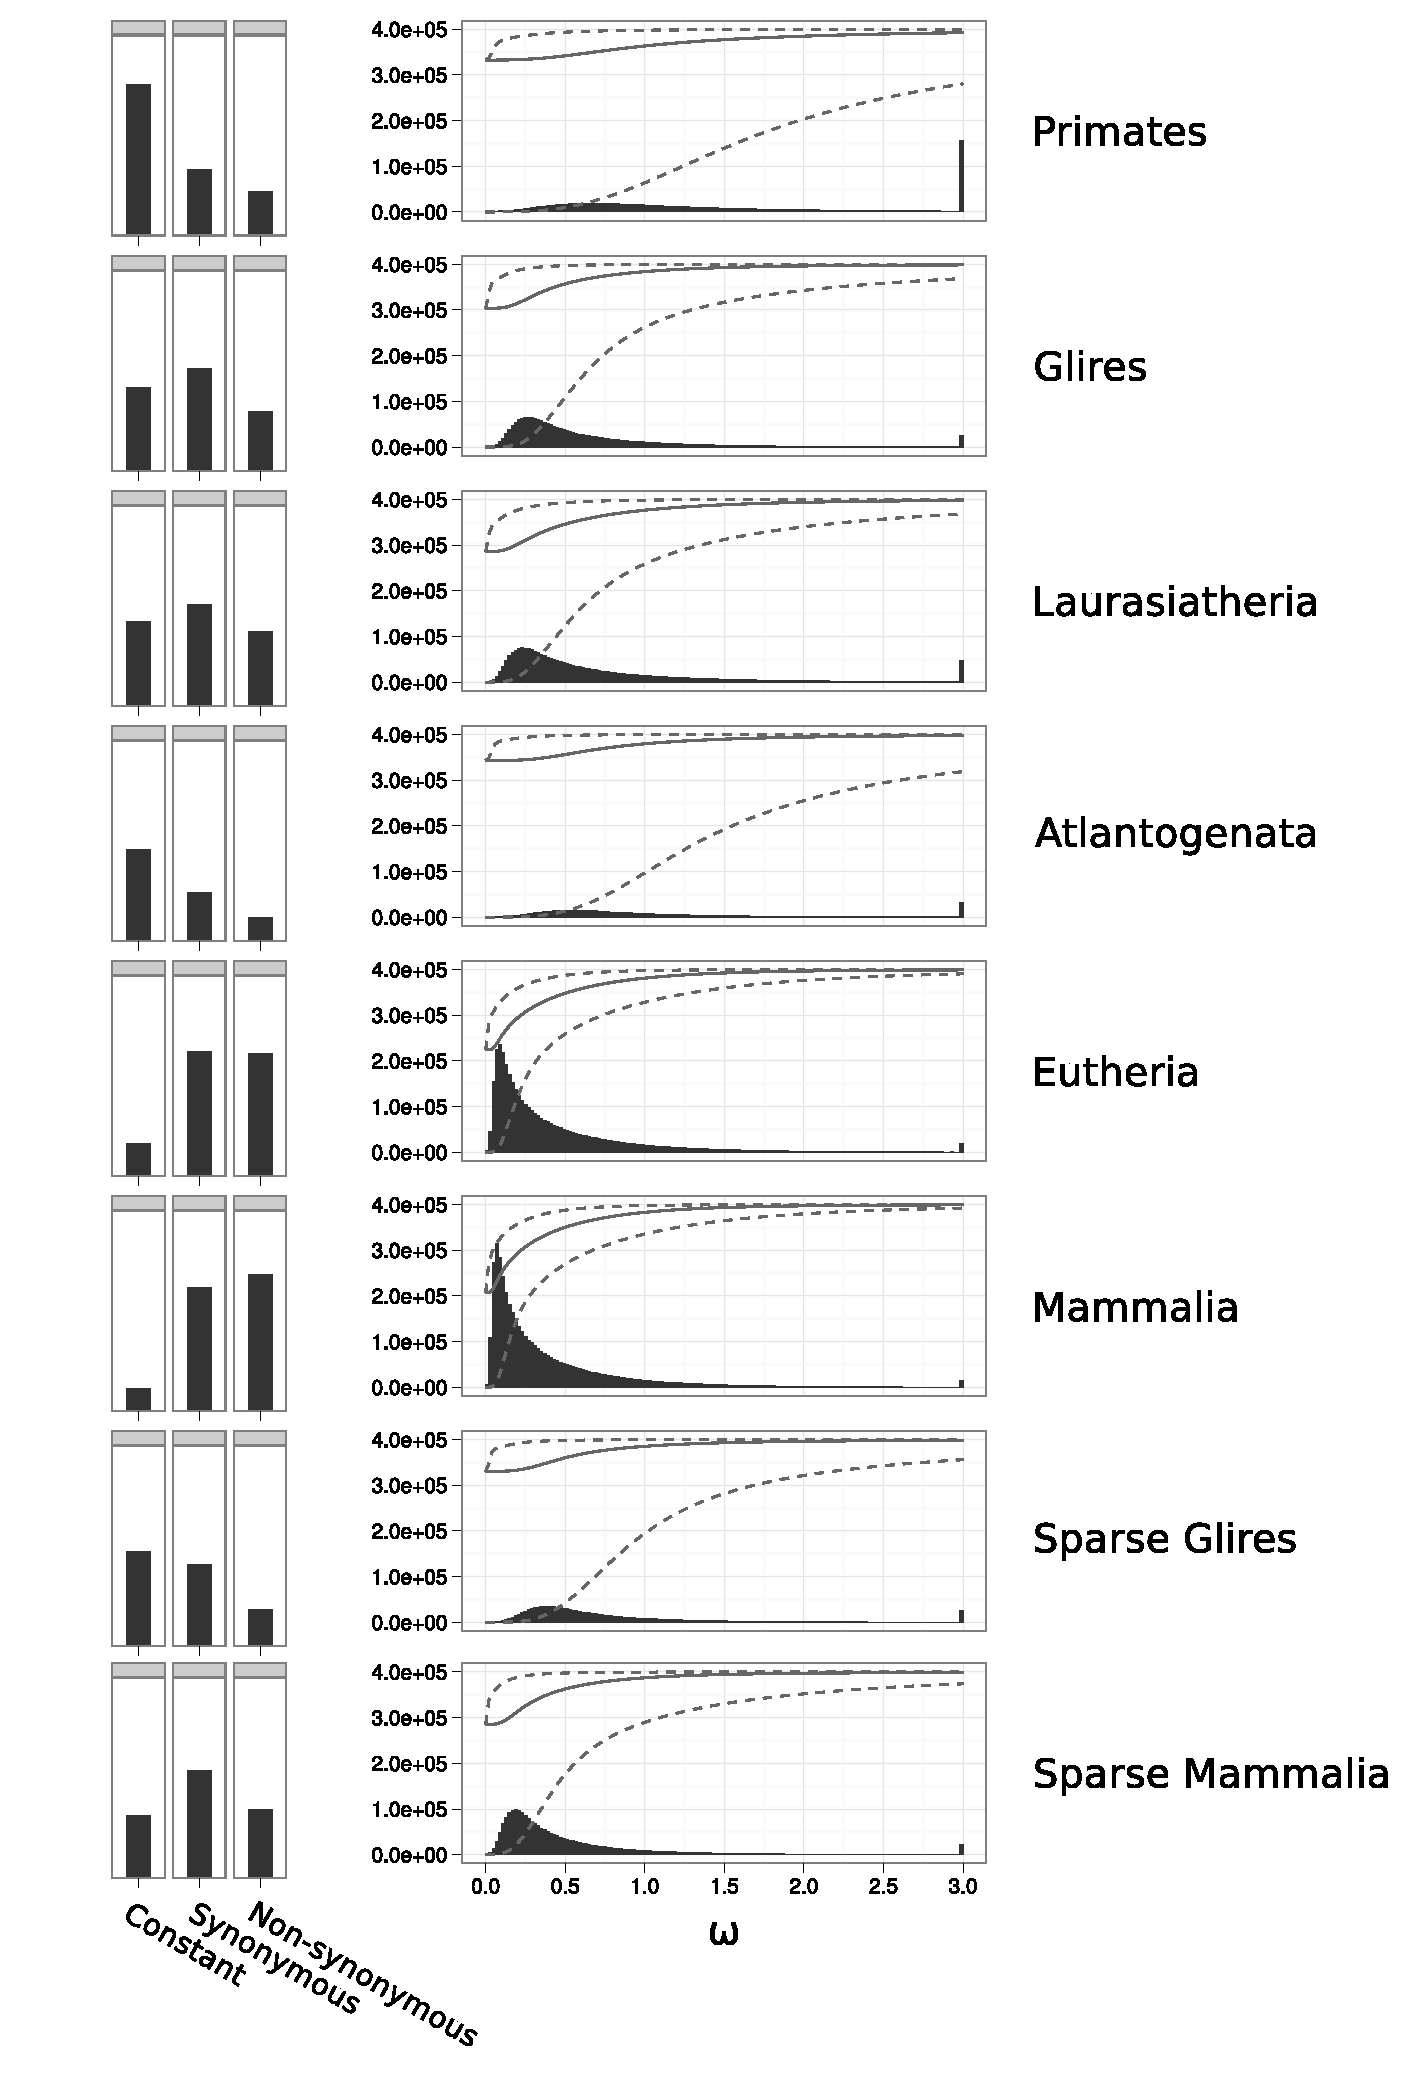
\includegraphics[scale=0.42]{Figs/global_distributions.pdf}
\caption{\scriptsize Global distributions of site patterns and \omg
  estimates for 10 species groups. Left panels: bars represent the
  number of sites showing constant, \syn, and \nsyn patterns. Note,
  the $y$-axis is held constant between rows. Right panels: bars
  represent histograms of \omgml estimates only for sites where
  \omgml$>0$. Sites with \omgml$>0$ correspond to sites with \nsyn
  site patterns, and sites with \omgml$=0$ correspond to constant or
  \syn site patterns. Sites with \omgml$>3$ are counted in the bin at
  \omgml$=3$. A solid line is drawn showing the cumulative
  distribution of \omgml, and dashed lines are drawn above and below
  the solid line showing the cumulative distributions of the lower and
  upper bounds, respectively, of the 95\% confidence interval
  associated with each \sw estimate.}
\label{fig_global_distributions}
\end{figure}

To produce high-confidence \sw estimates across the 10 chosen species
groups, sitewise data from each species group were processed with the
conservative filter as described above. The resulting global
distributions of site patterns, sitewise \omgml estimates, and 95\%
confidence intervals are shown in Figure
\ref{fig_global_distributions}. The left panel in each row shows the
number of sites with constant, \syn, and \nsyn patterns; all sites
with \omgml$=0$ had constant or \syn patterns, and all sites with
\omgml$>0$ had \nsyn patterns. The right panel in each row shows the
distributions of \omgml for sites which contained a \nsyn site
pattern.

The site pattern counts in Figure \ref{fig_global_distributions}
showed that the branch length of each species group had a strong
effect on the overall composition of the sitewise data. Groups
covering little branch length, such as Primates and Atlantogenata,
contained mostly constant sites, while groups covering a large amount
of branch length, such as Eutheria and Mammals, contained few constant
sites and roughly equal proportions of sites with \syn and \nsyn site
patterns.

The distributions of \omgml estimates are shown in Figure
\ref{fig_global_distributions} as a series of histograms showing the
\omgml density (for \nz values of \omgml only) and a series of solid
lines showing the cumulative \omgml density (representing all values);
the lower and upper dashed lines show the cumulative densities of the
lower and upper limits of the 95\% confidence interval resulting from
each \sw estimate. It was clear that the majority of protein-coding
sites have evolved under purifying selection in mammals, a fact which
was most easily seen in the species groups with large total branch
length. The Mammals group showed a maximum density of \nz \omgml
estimates at $\omega\approx0.1$, and the vast majority of sites showed
some evidence of purifying selection with \omgml$<1$.

The \nz \omgml values were more evenly spread in the other species
groups: Glires contained a maximum \nz \omgml density at around
$\omega\approx0.25$ and Primates at $\omega\approx0.7$. This upwards
shift in \nz \omgml estimates relative to Mammals was likely due to
the greater proportion of constant and \syn sites in datasets with
lower overall branch lengths: sites which were truly evolving with
$0<\omega<1$, but where no \nsyn or \syn substitutions were observed,
would have their \omgml estimate ``pushed'' towards zero, presumably
causing an apparent upwards shift in the distribution of the remaining
\nz \omgml values.

\section{Identifying sites with significant evidence for purifying and positive selection}
\label{section_pos_pur}

An important component of SLR's output is \sw information indicating
the confidence with which purifying or positive selection was
detected. These values include the lower and upper bounds of \ci, the
95\% confidence interval for each \omgml estimate, and the LRT
statistic, which corresponds to the strength of evidence for purifying
or positive selection.  sites with \slrt$<0$ showed at least some
evidence for purifying selection, and sites with \slrt$>0$ showed at
least some evidence for positive selection. It should be noted that
the \slrt is a measure of the strength of evidence for purifying or
positive selection, not of the actual strength of that selection. For
example, an alignment covering a very large branch length might yield
a strongly negative \slrt for a site with \omgml only moderately below
1, because the evidence for purifying selection at that site was
highly statistically significant; on the other hand, a
strongly-purifying site in an alignment covering less branch length
might produce a much less-negative \slrt, even with an estimated
\omgml near zero.

\begin{figure}[t!]
\centering
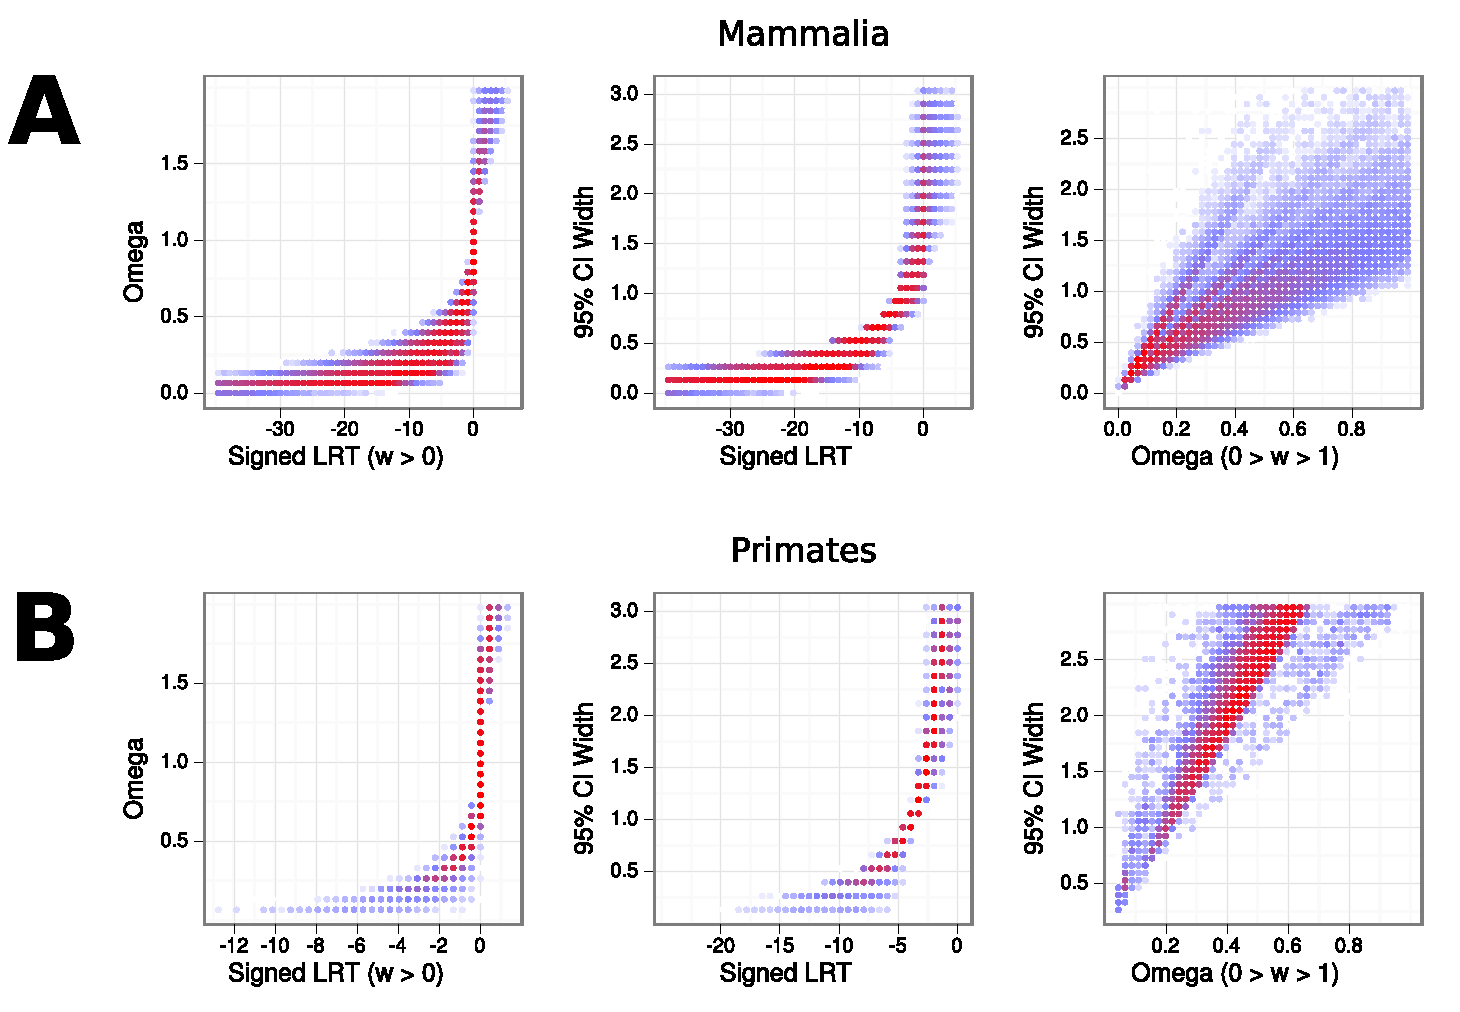
\includegraphics[scale=0.5]{Figs/sites_scatters.pdf}
\caption{The relationship between \slrt, \omgml, and \ci width in (A)
  Mammals and (B) Primates datasets. Each point represents the binned
  density of sites; no points are drawn where no density exists, while
  blue and red points are drawn at areas of low and high density,
  respectively. The left panel shows sites where \omgml$>0$, the
  middle panel shows all sites, and the right panel shows sites where
  $0<$\xspace\omgml$<1.3$. Note the change in $x$-axis scales between plots
  in (A) and (B), reflecting the paucity of sites in Primates with
  strong evidence (\slrt$<$-12) for purifying selection.}
\label{fig_sites_scatters}
\end{figure}

Figure \ref{fig_sites_scatters}A shows the relationship between \slrt,
\omgml and the \ci width for sites from the Mammals group. The left
panel, comparing the \slrt to \nz \omgml estimates, shows that the two
values are highly correlated, with the greatest number of low \omgml
estimates occurring at sites with strongly negative
\slrt. Correspondingly, the middle panel shows an even stronger
relationship between the \slrt magnitude and the \ci width, with the
tightest confidence intervals at sites with very strong evidence for
purifying selection. The rightmost panel compares the \omgml of each
site with the width of its \ci, revealing a more linear and diffuse
positive relationship between \omgml and the size of the \ci. The
equivalent plots for Primates, shown in Figure
\ref{fig_sites_scatters}B, reveal similar patterns, but with generally
less-negative \slrt values, higher \omgml, and larger \ci. These
differences highlight the impact of branch length on the amount of
confidence with which \omg can be estimated on a per-site basis. The
low branch length of the Primates clade rarely yields \omgml estimates
with \ci intervals smaller than 1, while the bulk of sites from the
Mammals dataset have relatively small \ci. Thus, the distribution
of \omgml estimates from datasets with low branch lengths (e.g., the
histogram densities seen in the top few panels of Figure
\ref{fig_global_distributions}) should be interpreted with caution, as
any comparison between \omgml from different sites or datasets may be
more sensitive to the amount of statistical confidence placed on each
estimate than to any meaningful biological difference between the two
sets of data.

\bbtable
\scriptsize{ \centering
\begin{tabular}{lllrrrrrrrrrrrrr}
\toprule
 &  & &  \multicolumn{3}{c}{Site Pattern, \%} & Med. & 
  \multicolumn{3}{c}{Nongap BL} & \multicolumn{2}{c}{\omgml} &
\multicolumn{4}{c}{\omgml Below / Above, \%} \\
\cmidrule(r){4-6} \cmidrule(r){8-10} \cmidrule(r){11-12} \cmidrule(r){13-16}
Name & Filter & Sites & Const. & Syn. & Nsyn. & Codons & Med. & Mean & SD & Mean & SD &
$< 0.5$ & $< 1$ & $> 1$ & $> 1.5$ \\
  \midrule
\input{Tables/pset_summaries_stringent_1.txt}
\bottomrule
\end{tabular}
\caption{\scriptsize Summary statistics of \sw estimates for all
  species groups with the conservative filter applied. Columns under
  the ``\omgml Below / Above'' heading measure the percentage of sites
  with \omgml below or above the indicated value. Med.---median;
  Const.---constant; Syn.---\syn; Nsyn.---\nsyn; BL---branch length; SD---standard deviation.
\label{table_pset_summaries_1}
}

\hspace{.2in}

\centering
\begin{tabular}{llrrrrrrrrrrrrrrrrrrrrr}
\toprule
 & & \multicolumn{8}{c}{Positively Selected Sites (\%)} &
\multicolumn{3}{c}{\chisqlt{0.1}, \%} &
\multicolumn{3}{c}{\chisqlt{0.05}, \%} \\
\cmidrule(r){3-10} \cmidrule(r){7-10} \cmidrule(r){11-13} \cmidrule(r){14-16}
Name & Filter & 
  \multicolumn{2}{c}{\chisqlt{0.1}} & \multicolumn{2}{c}{\chisqlt{0.05}} &
  \multicolumn{2}{c}{\chisqlt{0.01}}& \multicolumn{2}{c}{\bhfdr{0.05}} &
  Neg. & Neut. & Pos. & Neg. & Neut. & Pos. \\
%\cmidrule(r){2-3} \cmidrule(r){4-5} \cmidrule(r){6-7} \cmidrule(r){8-9}
\midrule
\input{Tables/pset_summaries_stringent_2.txt}
\bottomrule
\end{tabular}
\caption{\scriptsize Proportions of sites subject to positive,
  purifying and neutral selection at various \slrt thresholds. The
  method of \citet{Benjamini1995} was used to identify the \slrt
  threshold at which FDR$<$0.05. For columns under the headings
  ``\chisqlt{0.1}, \%'' and ``\chisqlt{0.05}, \%'', Pos. and Neg. are
  the percentage of sites with significant evidence for positive and
  negative selection, respectively, and Neut. is the percentage of
  ``neutral'' sites not showing significant evidence for non-neutral
  selection.}
\label{table_pset_summaries_2}
}
\eetable

Instead, the confidence intervals and \ac{lrt} statistics calculated
by \ac{slr} for each site can be used to identify sites evolving
under purifying or positive selection with confidence. Sites with
\ciup, the upper bound of the \ci interval, below \omg$=1$ could be
interpreted as having evidence of purifying selection with an expected
5\% \fpr; likewise, sites with \cidown above \omg$=1$ contained
evidence of positive selection with an expected 5\% \fpr. In both
cases, \ac{slr} was controlling for an expected 5\% \fpr under the
null model of neutral evolution. As expected, there was a direct
relationship between \ciup and the \chisq approximation to the \slrt
distribution, whereby the set of sites with \ciup$<1$ was exactly
equivalent to the set of sites with \slrt below the negative \chisq
95\% critical value. Similarly, the sites with \cidown$>1$ were those
with \slrt above the \chisq 95\% critical value. Because of this
equality, I will refer to \slrt values at various \chisq threshold
values instead of the 95\% \ci intervals when discussing sites with
significant evidence for purifying or positive selection.

Tables \ref{table_pset_summaries_1} and \ref{table_pset_summaries_2}
provide summaries of the sitewise estimates obtained for each of the
10 mammalian species groups using conservative filtering, showing the
same statistics provided earlier in Tables
\ref{table_filter_summaries_1} and \ref{table_filter_summaries_2} for
the different filters.

Table \ref{table_pset_summaries_2} presents the proportions of
\acp{psc} identified at a variety of \slrt thresholds and in different
species groups, demonstrating that anywhere between 0.01\% to 0.73\%
of sites were identified as under positive selection, depending on the
nominal \ac{fpr} threshold and the species group used.

Different species groups yielded strikingly different estimates of the
proportion of \acp{psc}. At a 5\% \ac{fpr} threshold, the Primates, HQ
Mammals, Laurasiatheria, Eutheria, and Mammals groups produced broadly
comparable proportions of positively-selected sites, ranging from
0.33\% to 0.42\%. The proportions of \acp{psc} in these groups were
higher using a 10\% \ac{fpr} threshold (ranging from 0.46\% to 0.73\%)
and lower using a 1\% \ac{fpr} threshold (ranging from 0.07\% to
0.19\%). When the FDR was controlled using the \citet{Benjamini1995}
method, however, far fewer \acp{psc} were identified. Only the
Eutheria and Mammals groups yielded a substantial number of
positively-selected sites at this level of control; the Primates and
Laurasiatheria data yielded non-zero numbers of \acp{psc} as well, but
these species groups were likely limited in their power to yield
positively-selected sites after FDR control due to their lower total
branch lengths.

The Atlantogenata, HMRD, Sparse Glires, Glires and Sparse Mammals
groups all produced lower proportions of positively-selected sites
identified across all \fpr thresholds. At FDR$<$0.05, all four groups
yielded zero significant \psc{}s, and at a 1\% \ac{fpr} they all
contained lower than 0.01\% \acp{psc}. These species groups were
widely distributed in the amount of total branch length they covered
(ranging in median \ngap branch length from 0.94 for Atlantogenata to
2.55 for Sparse Mammals), suggesting that the lower number of
\acp{psc} was not strongly influenced by branch length; a similar
point could be made of the species groups with higher proportions of
\acp{psc}, which comprised the groups with both the lowest (Primates)
and the highest (Mammals) total branch lengths.

In Mammals, the breakdown of sites into positive, negative and neutral
categories at 10\% and 5\% significance thresholds produced a pattern
similar to that seen in the \omgml distributions from Figure
\ref{fig_global_distributions}. A large amount of purifying constraint
(83.87\% of sites at 5\% FPR), a smaller proportion of
neutrally-evolving sites (15.57\%), and a diminishing fraction of
positively-selected sites (0.55\%) were observed. As expected given
the use of a fixed \slrt threshold to identify purifying sites, the
fraction of sites confidently identified as under purifying selection
showed a strong dependency on the branch length of the species set,
with a much higher power in Mammals than in Primates to confidently
detect purifying selection (83.87\% vs.\ 15.97\%).

\section{The impact of \ac{ne} on protein-coding constraint in mammals}

Overall, the conservatively-filtered \sw data showed that, when using
\omgml estimates, between 1\% to 5\% of protein-coding sites are
evolving under positive selection. This number varied strongly between
different species groups, however. Comparing between the four
phylogenetically independent mammalian superorders (Primates, Glires,
Laurasiatheria, and Atlantogenata), I found that Primates showed by
far the most \acp{psc} and sites with \omgml$>1$. Laurasiatheria
showed similar proportions of sites with \omgml$>1$, but Atlantogenata
showed fewer \acp{psc} than Laurasiatheria. The Glires group showed
strikingly lower levels of positive selection compared to the other
mammalian superorders. Despite the relatively large amount of branch
length covered by the Glires group (median total length of 1.77,
versus 2.03 for Laurasiatheria), only 0.10\% of sites were identified
as \acp{psc} in Glires at a 5\% \ac{fpr}, compared to 0.33\% in
Laurasiatheria and 0.41\% in Primates.

These results may be evaluated in terms of the impact of \ac{ne} on
the efficacy of natural selection in mammals
\citep{Popadin2007,Nikolaev2007,Ellegren2009}. Rodents are known to
have \ac{ne} well above that of primates \citep{Kosiol2008}, and given
the strong correlation between body size, generation time and \ac{ne}
\citep{Nikolaev2007} one can infer that species within the
Laurasiatheria group, with generally longer generation times and
larger body sizes than rodents \citep{Hou2009}, have \ac{ne} more
similar to those seen in primates. The Afrotheria group, containing
species ranging from small moles to elephants and manatees, is more
diverse, making it difficult to estimate an expected historical
\ac{ne}. Nevertheless, Ohta's nearly neutral theory \citep{Ohta1992}
predicts that species with lower \ac{ne} will evolve with less
efficient natural selection. A comparison of the Primates and Glires
data clearly revealed this effect: the proportion of sites with
\omgml~$<0.5$ was 87.27\% for Primates and 90.54\% for Glires. Thus,
differences in the proportion of sites under purifying selection were
well explained by the difference in \ac{ne} between primates and
rodent-like mammals.

Theory also predicts that positive selection should be more efficient
in populations with high \ac{ne} \citep{Ellegren2009,Halligan2010},
and a number of empirical studies have supported this prediction. The
prevalence of adaptive evolution has been extensively studied in
different species using a combination of within-species diversity and
between-species divergence data, finding high proportions of amino
acid substitutions driven by positive selection in species with high
\ac{ne} such as \emph{Drosophila} \citep{Bierne2004} and
\emph{E. coli} \citep{Charlesworth2006}, and low proportions in
species with low \ac{ne} such as human
\citep{Zhang2005b,Sequencing2005a,Boyko2008} and chicken
\citep{Axelsson2009}. Fewer studies have assessed differences in
levels of positive selection between species using only divergence
data and \dnds-based tests for selection, but some such analyses have
been published. \citet{Clark2007} used \acs{paml} \citep{Yang2007} to estimate the
proportion of \acp{psg} and \acp{psc} in 12 \emph{Drosophila} genomes,
finding evidence for positive selection within 33\% of single-copy
orthologs, affecting 2\% of codons within those
\acp{psg}. \citet{Kosiol2008} found a lower proportion of \acp{psg} in
their analysis of 6 mammalian genomes, with only 544 candidate
\acp{psg} out of 16,529 orthologs tested (3.3\%). The authors then
compared the levels of apparent positive selection in different
lineages, finding that 72\% of the 544 candidate \acp{psg} showed
evidence of positive selection in rodents; they concluded that
``whether because of power or a genuine increase in selection, the
rodent branch appears to play a major role in the identification of
PSGs'' \citep{Kosiol2008}. Together, these two studies based on \dnds
estimates largely support the theoretical prediction of increased
levels of positive selection in populations with large \ac{ne}.

The current results appeared to contradict the theoretical prediction
and empirical evidence for a positive correlation between \ac{ne} and
the prevalence of positive selection in mammalian species. The
Primates, Laurasiatheria and HQ Mammals species groups showed greater
levels of positive selection than the Glires group, as measured by
both the proportion of sites with \omgml$>1$ and the proportion of
\acp{psc} identified at all \ac{fpr} and \ac{fdr} thresholds shown in
Table \ref{table_pset_summaries_2}. These species groups were the same
groups which showed evidence for lower long-term \ac{ne} due to their
elevated mean \omgml values and decreased proportion of sites with
\omgml$<1$ (Table \ref{table_pset_summaries_1}). Although estimates of
\omgml should be treated with caution due to stochasticity in the
\ac{ml} estimate at a single alignment site, further evidence for
lower \ac{ne} in these species groups came from the estimates of
gene-wide \dnds values calculated by \ac{slr} based on the M0 codon
model of evolution. Figure \ref{fig_mammals_dnds_ratios} shows a
comparison of gene-wise \dnds in these species groups, providing
strong evidence for the following ordering of \ac{ne}:
Glires~$>$~Laurasiatheria~$\approx$~Atlantogenata~$>$~Primates. Thus,
rather than a positive correlation between \ac{ne} and the prevalence
of positive selection, these \sw data seemed to exhibit a negative
correlation between these two factors.

\begin{figure}[t!]
\centering
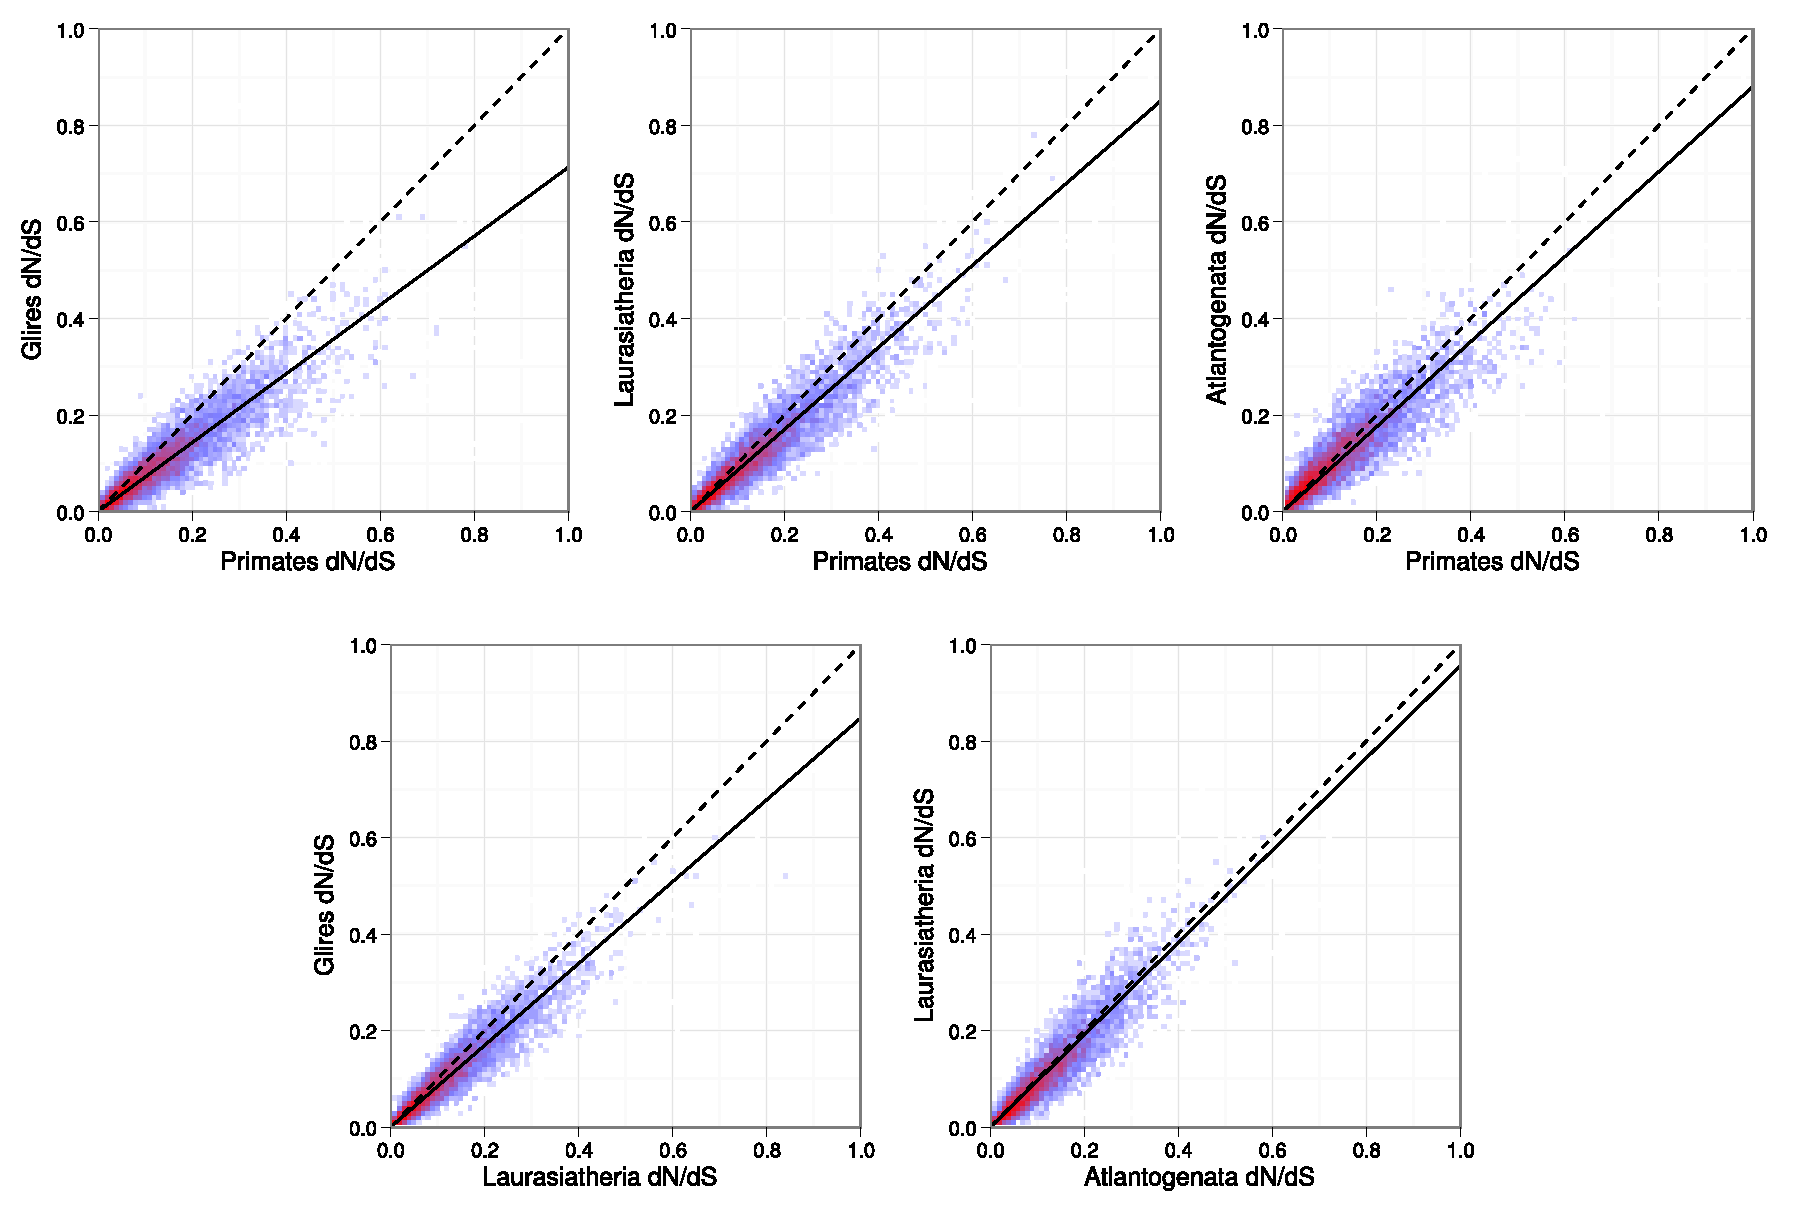
\includegraphics[scale=0.5]{Figs/mammals_dnds_ratios.pdf}
\caption{Correlations between gene-wide \dnds ratios estimated for
  \ntrees orthologous genes in four different species groups. \dnds
  ratios were estimated for each alignment by \ac{slr} using the M0
  (one ratio for all sites) codon model of evolution. Genes were
  plotted according to their \dnds ratio in each species group, and
  each panel shows the density of genes as a colored heat map with red
  areas corresponding to the highest density of points. A dashed line
  with slope of 1 is drawn for reference, and a solid line is drawn in
  each panel along the first principal component axis of those data
  points.}
\label{fig_mammals_dnds_ratios}
\end{figure}

This suggested an alternative interpretation: that perhaps the
different levels of positive selection could be due mainly to the
relaxation of selective constraint in Primates and other species with
low \ac{ne}. A difference in \ac{ne} should impact slightly
deleterious and slightly advantageous mutations equally, with a
greater proportion of both types of mutations being effectively
neutral in the population with lower \ac{ne}. In comparing the
Primates and Glires groups, the expected result was that a subset of
mutations which were under purifying selection in Glires would be
effectively neutral in Primates, bringing the expected \omg for those
sites from $<1$ to 1. The same should occur for slightly advantageous
sites, but if the proportion of slightly deleterious sites is much
greater than the proportion of slightly advantageous sites, it may
have a much more measurable impact. Furthermore, since sites with
\dnds$=1$ are more likely to produce false positive \acp{psc}, it is
plausible that the greater proportion of effectively neutral sites in
a species with low \ac{ne} would lead to an increased proportion of
\acp{psc} detected by methods based on \dnds ratios.

This relaxed constraint argument tempers the interesting observation
of strong differences in the numbers of \acp{psc} between different
species groups. A lower historical \ac{ne} for the Primates and
Laurasiatheria species groups may explain some of the increase in the
number of \acp{psc} detected, even in the absence of true variation in
the prevalence of positive selection between the species groups
investigated here.

Still, the argument may be made that statistical methods for
controlling error rates, such as the \citet{Benjamini1995} method for
FDR control used to identify \acp{psc} at an expected FDR$<0.05$ in
Table \ref{table_pset_summaries_2}, should account for the potential
confounding effects of relaxed constraint noted above. For this
reason, the observation that Primates and Laurasiatheria both yielded
non-zero numbers of \acp{psc} at FDR$<0.05$ may be taken as some
indication of a true difference in the levels of positive selection
between the species groups investigated here. This apparent
discrepancy with previously-published results should be an interesting
area for continued investigation.

\section{Conclusions}

This chapter described the filtering, alignment, and analysis of \sw
selective pressures in a comprehensive set of orthologs across 38
mammalian species. In order to ensure that false signals of positive
selection were avoided as much as possible, several levels of
filtering were applied before and after the estimation of \sw
selective pressures using \ac{slr}: low-quality genomic sequence was
masked out, short or divergent apparent paralogous gene copies were
removed, and alignment columns showing evidence of clustered \nsyn
substitutions or low amounts of evolutionary information were excluded
from the analysis. A comparison of the levels of purifying and
positive selection contained within sites filtered at various
thresholds showed the importance of thorough filtering prior to
genome-wide analysis, highlighting especially the ability of stretches
of mis-annotated or mis-assembled sequence to introduce strong (and
incorrect) signals of localized positive selection. I showed that a
novel approach, based on the identification of lineage-specific
clusters of excessive \nsyn substitutions within short alignment
windows, could effectively target these erroneous regions for removal.

Sitewise selection pressures were then calculated for several groups
of mammalian species. The impact of the total branch length of a
species group on the estimation of \sw selective pressures could be
clearly seen from these results, with the Mammals group containing
many more non-constant alignment sites and a more accurate
distribution of \omgml estimates than groups with little total branch
length, due to the greater amount of evolutionary information.

The \ac{mgp} analysis consortium used the HMRD and HQ Mammals groups
as reference points by which to estimate the increase in power to
detect genome-wide constraint resulting from the additional mammals
sequenced at low coverage. Comparing \sw results to the same reference
species groups, I found that the addition of \lcv genomes increased
the ability to detect purifying constraint in protein-coding regions
by 43.85\% and 136\% compared to the HQ Mammals and HMRD species
groups, respectively, at a 5\% \ac{fpr}. Although I found the levels
of positive selection between species groups to be highly dependent on
the species sampling (and thus, a comparison of ``power'' to be less
meaningful), the Mammals species group identified 21.5\% and 550\%
more \acp{psc} than the HQ Mammals and HMRD species groups,
respectively, at a 5\% \ac{fpr}. Thus, the additional branch length
resulting from the sequencing of \lcv genomes greatly improved the
power to detect purifying and positive selection in mammalian
proteins.

Finally, I analyzed the levels of purifying and positive selection
within four phylogenetically independent mammalian species groups,
identifying strong differences in levels of purifying and positive
selection in different groups, likely resulting from differences in
\ac{ne}. Although the impact of \ac{ne} is well known and has been
previously studied in mammalian species, the work described in this
chapter represented a careful and quantitative analysis of levels of
purifying and positive selection in these species groups. The
observation that the Glires group showed less positive selection than
all other groups suggested a connection between high numbers of
\acp{psc} and relaxed constraint, although Primates and Laurasiatheria
both showed evidence for strong \acp{psc} even at a very stringent FDR
threshold.

More work needs to be done to evaluate what might be causing these
strongly different estimates in different mammalian superorders and to
correctly control for the possible effect of relaxed constraint on the
identification of positive selection in primate genomes. Differences
between the current results and those obtained from diversity-based
estimates in contemporary populations could be attributed to
differences in the timescale under examination \citep{Ellegren2009},
as divergence-based estimates of selective constraint are obviously
sensitive to the long-term \ac{ne} within each clade, while
diversity-based estimates measure the selective constraints based on
more recent \ac{ne}. However, the contrast with the results of
\citet{Kosiol2008}, who used similar \dnds based methods yet found
higher levels of positive selection in the rodent lineage than the
primate lineage, is less easily explained.

An interesting question for future work is whether the observed
species group differences in positive selection result more from
differences in ancient or more recent branches in the phylogeny. In
other words, at what point in evolutionary time did the major
mammalian orders begin to experience different levels of positive
selection (or relaxed constraint)? Although these groups of species
show different contemporary \ac{ne}, they have evolved independently
for several dozen million years, during which time several \ac{ne}
expansions or contractions could have occurred. With more dense
species sampling and branch-specific \dnds estimates, a clearer
picture of the connection between the evolution of \ac{ne}, relaxed
constraint and positive selection may begin to emerge.

\tocite{Eory et al. 2010}{Showed, through constraint analysis of
  various sequence types, that there is higher selective constraint in
  4-fold sites in primates compared to murids. Quote: ``It is well
  established that in several organisms, mutations at 4-fold sites are
  selected against (Chamary et al. 2006; Rocha 2006; Drummond and
  Wilke 2008) and as a consequence the dN/ds ratio, which has been
  frequently used to detect the strength and direction of selection
  (e.g., Dorus et al. 2004; Wang et al. 2006), may be
  underestimated. Our result of higher 4-fold constraint in hominids
  suggests that this bias more strongly affects hominid estimates and
  it may well exceed 20\%.''}

\tocite{Ohta 1993, 1995; Eory et al. 2010}{The Keightley et al. 2011
  paper (ABC to estimate mutation rate parameters) cited Ohta 1993,
  1995 and Eory et al. 2010 for the effective population size and
  efficacy of selection in primates vs.\ murids}

\tocite{Wolf et al. 2009}{Wolf et al. GBE 2009, used pairwise dN dS
  counts to try to show that trends in dN/dS ratios are a result of
  branch length, at least when calculated in a pairwise
  fashion. Slightly unconvincing stuff... could be cited as somehow
  relating to the discussion regarding eff. pop. size, branch length,
  and selection}

\tocite{Berglund et al. 2009}{Berglund et al. 2009 looked at hotspots
  of biased substitutions in humans. Showed that exons with
  accelerated rates in humans have a tendency towards clusters of
  AT-to-GC (weak-to-strong) substitutions. Did some simulations
  showing that this effect is strongest in GC-poor regions, though the
  impact on overall dN/dS is probably minimal (e.g., genes with
  overall high dN/dS didn't show BGC, only the most accelerated exons
  did) and the effect on dN/dS is highest in high-GC regions. The
  most-accelerated exons tend to reside in high-male (but not female)
  recombination, and <50kb from hotspots. Upshot: these biased
  clusters seem to show up in isolated regions (exons), rather than
  spread throughout entire genes. Probably not a huge impact on
  overall apparent constraint.}

\tocite{Duret and Arndt PLoS Gen 2008}{Duret and Arndt 2008 use
  nonreversible nucleotide models to estimate NEUTRAL rates correlated
  with recombination, GC, and GC*. Lots of stuff here, but the
  important bits: overall mutation rate increases with increasing GC
  content (due to overall higher rates of S-W substitution);
  recombination should have a strong impact on W-S substitution, but
  weak impact on S-W substitutions; CpG deamination varies by factor
  of two, very low in GC-poor regions and very high in GC-rich ones.}

\tocite{Galtier et al. TrIG 2009}{Galtier et al. TRIG 2009 is similar
  to Berglund et al. in many ways -- find accelerated exons in a
  primate branch, and identify significantly higher male recombination
  rates there. The number of accelerated exons is small -- ~100 in
  each of four branches -- and not all of these accelerated exons
  showed strongly elevated dN/dS ratios. Only 19 exons at the 1\%
  level. However, they do some nice modeling (mostly in the
  supp. material) which shows that the effect of BCG on dN/dS ratio at
  different GC contents -- it has more effect in GC-rich genes.}

\tocite{Capra and Pollard 2011}{Capra and Pollard quantified BDS
  (biased divergent substitutions) across metazoans, additionally
  using recombination rate data. Dog has the strongest, mouse has the
  weakest BDS scores. (This could be due to lower rec. rate in mouse,
  e.g. Coop and Przeworski 2006)}

\tocite{Nordborg et al. 1996}{Nordborg et al. 1996 (Genet. Res.)
  modeled the effect of background selection on variation in neutral
  linked loci. They showed that weakly selected mutations, rather than
  strongly selected ones, are more likely to produce regional
  patterning of variation in response to local recombination
  rate. Should have a large effect in Drosophila but small effect in
  mammals, though in mammals ``local reductions in regions of reduced
  recombination might be detectable.''}

\tocite{Chun and Fay 2011}{Chun and Fay 2011 (PLoS Gen) looked at
  neutral and deleterious SNP density according to local recombination
  rate, showing that in 'hitchhiking' regions there are fewer neutral,
  but as many deleterious, polymorphisms. That stuff is boring, but
  they also show that the deleterious SNP density stays constant
  throughout the range of recombination rates, while the neutral and
  synonymous SNP density decreases. Thus, slightly deleterious
  mutations are less effectively purged in regions of low
  recombination.}

\tocite{Bullaughey et al. 2008}{Bullaughey et al. (2008, Gen. Res.)
  looked at gene-wide dN/dS ratios in primates and recombination
  rates. They found no significant correlation between broad- or
  fine-scale recomb. rates and rates of protein evolution, **once GC
  content is taken into account**.}

\tocite{SPencer et al. 2006}{Spencer et al. (2006 PLoS Gen) Quote: ``In short,
  while there is a strong relationship between recombination and GC
  content, most of the relationship is explained by scales broader
  than recombination hotspots (16 to 256 kb; unpublished data) and may
  well result from interactions of both factors with additional
  processes such as chromatin organisation or replication
  timing. Similar arguments apply to the question of whether a GC bias
  in recombination-associated mutation can explain the relationship
  between GC content and recombination.''}


%************************************************
\chapter{Characterizing the evolution of genes and domains in mammals using \sw selective pressures}
\acresetall
\label{ch_mammals2}
%************************************************
\section{Introduction}

This chapter describes the use of \sw data to identify trends in the
evolution of protein-coding genes and domains, focusing on the
detection of \acp{psg}. I will first develop a number of methods for
using \sw estimates to identify signals of positive selection within
genes and domains and apply these methods to the \sw data generated in
Chapter \ref{ch_mammals1}. Next, to provide a higher-level
interpretation of these results I will use functional gene annotations
to identify categories enriched for genes with evidence of positive
selection in different species groups. Lastly, I will place these
results within the context of the literature by cirectly comparing the
sets of \acp{psg} identified by this and previously-published studies.

Since the first non-human mammalian genomes were sequenced, there has
been great interest in using comparative data to identify genes
showing signatures of positive selection in mammals. Much of this
interest stems from the prospect that such genes may reflect the
historical impact of natural selection acting to fix beneficial
mutations within a population over time---a major driving force in the
modern molecular interpretation of Darwin's theory of natural
selection \citep{Endo1996,Hughes1999}. Previous scans for positive
selection in primate genomes have revealed enrichments for \acp{psg}
related to sensory perception and olfaction \citep{Clark2003},
apoptosis and spermatogenesis \citep{Nielsen2005}, and iron ion
binding and keratin formation \citep{Macaque2007}; analyses in other
mammalian genomes have revealed largely similar patterns
\citep{Kosiol2008,Li2009a}. To explain the increased \dnds values
observed within \acp{psg}, three distinct evolutionary dynamics have
commonly been invoked: an evolutionary arms race between host and
parasite interacting genes \citep{Yang2005c,Meyerson2011}, sexual
selection or genetic conflict between the sexes
\citep{Wyckoff2000,Clark2000}, and functional adaptation following
gene duplication \citep{Zhang2002}.

As the power of phylogenetic analysis using codon models depends
strongly on the amount of branch length encompassed by the species
being compared \citep{Anisimova2001,Anisimova2002}, there was some
reason to believe \emph{a priori} that the detection of \acp{psg}
using mammalian alignments incorporating \lcv genomes would be more
powerful than in previous whole-genome analyses, which typically
included 12 or fewer species across mammals and lower total branch
length \citep{ELLEGREN2008k}. However, differences in the specific
models used to detect positive selection are expected to affect the
sensitivities of one study compared to another \citep{Anisimova2009},
so the set of genes identified using the current methodology would
necessarily be expected to be a superset of those identified in
previous studies. Most large-scale studies have used the branch-site
test for positive selection \citep{Zhang2005}, while the results
described in this chapter were generated using \ac{slr}. I showed in
Chapter \ref{ch_indels1} that \ac{slr} has similar power to the
site-based test implemented in PAML for detecting \sw positive
selection, but no analysis has yet compared the differences in
\acp{psg} identified by site-specific and branch-site methods on a
large scale. For this reason, I hoped that a quantitative comparison
between \acp{psg} identified using the current methodology and those
found in previously-published studies may improve our understanding of
how similar or different the \acp{psg} identified by different methods
can be.

\section{Combining \sw estimates to identify positive selection}

In Chapter \ref{ch_mammals2} I covered the generation and analysis of
several highly filtered sets of genome-wide \sw selective pressures
within different groups of mammalian species. These \sw estimates were
used to characterize the global distribution of evolutionary
constraint and to compare overall levels of purifying and positive
selection between groups of mammalian species. The focus on individual
codons as an evolutionary unit of investigation is relatively
uncommon, but it allowed for large-scale differences in evolutionary
trends between species groups to be identified and for the impact of
different filtering schemes on overall signals of positive selection
to be easily evaluated.

The more traditional approach in comparative genomics has been to
model the protein-coding gene, as opposed the protein-coding amino
acid site, as the unit of analysis. For detecting positive selection,
the grouping of alignment sites into genes---which results in
identification of \acp{psg} instead of \acp{psc}---has three main
advantages. First, the combined analysis of many alignment sites
improves the accuracy of estimated evolutionary parameters and boosts
the power \ac{lr}-based tests for detecting positive selection. This
can be easily seen in the simulations of Anisimova and Yang
\citeyearpar{Anisimova2001,Anisimova2001}, which showed large power
differences for detecting positive selection in alignments simulated
with 100, 200, and 500 codons. Second, detailed studies of \sw
selective pressures in genes with strong signals of positive selection
have usually observed clusters of positively-selected sites
\citep{Sawyer2005a,Kosiol2008}, suggesting that the evolutionary
dynamics creating detectable signals of positive selection tend to
affect many functionally or structurally related amino acid sites
within a gene as opposed to a single site. These studies represent
empirical evidence that combining \sw estimates within genes is
biologically sensible. The third argument in support a gene-centric
analysis of positive selection is that in the absence of complete
protein structure information, much more tends to be known about
entire genes (through the results of high-throughput studies and
experiments in model organisms) than is known about individual
protein-coding sites. Thus, a gene-centric analysis allows a dataset
to be more easily analyzed in connection with abundant external
functional data, benefitting the biological interpretation of results.

A major issue in combining \sw estimates to identify \acp{psg} is that
of correcting for performing multiple \sw tests per gene. The \ac{slr}
method performs an independent statistical test at each site,
producing a sitewise statistic which can be compared to a \chisq
distribution to yield a p-value representing the strength of evidence
against strict neutral evolution \citep{Massingham2005}. When
combining these p-values to decide whether a gene contains significant
evidence for positive seletcion, one must take into account the number
of tests performed. For example, a 100-codon gene evolving under the
null model ($\omega=1$) would be expected to produce 5 sites with
p-values at a nominal \ac{fpr} of 0.05; correspondingly, the chance
that at least one site within the gene would have $p<0.05$ is
99.4\%. This is calculated as the complement of the probability that
no sites out of $n$ have $p<x$, which is $(1-x)^{n}$. Thus, if the set
of genes containing at least one site with nominal $p<0.05$ were
called \acp{psg}, nearly all genes evolving under the true null model
would be selected. In contrast, the \ac{lrt}s for positive selection
implemented in PAML only perform one statistical test per gene and do
not suffer from the same multiple testing problem. Clearly, some
procedure for correcting or combining the results from multiple tests
must be applied in order to identify \acp{psg} using \sw data in a
statistically controlled manner.

I tested 3 types of methods which are capable of correcting for
multiple \sw tests within genes to identify \acp{psg}: first,
adjusting significance thresholds to control the \ac{fwer}; second,
combining p-values from multiple tests to produce a single p-value
summarizing the overall evidence against the null hypothesis; third,
estimating empirical gene-wise p-values based on the genome-wide
distribution of \sw estimates. Each approach makes different use of
the \sw data from each gene to identify a set of significant \acp{psg}
and thus had the potential to yield a unique set of \acp{psg}. The
remainder of this section provides some background on each approach
and describes how it was applied to the current problem.

\subsection{Controlling the \ac{fwer}}

The \ac{fwer} is defined as the probability, for a given set of tests
performed, of one or more tests producing a false positive result. In
the example of a 100-codon gene evolving under the null model, the
\ac{fwer} at a nominal p-value of 0.05 was 0.994. Assuming an
appropriate uniform null distribution of p-values and independence
between tests, the \v{S}id\`{a}k equation (to which the more popular
Bonferroni correction is an easily computed approximation) identifies
the p-value threshold $x$ which is necessary to control the \ac{fwer}
at the desired level $\alpha$. The \ac{fwer} expected for a family of
$n$ tests thresholded at a nominal p-value of $x$ is $\alpha=1 - (1 -
x)^{n}$, so the p-value threshold necessary to control for a desired
\ac{fwer} can be found by rearranging the equation: $x=1 - (1 -
\alpha)^{1/n}$. A similar but more powerful approach to controlling
the \ac{fwer} is the step-up method from Hochberg; this method is
implemented internally by \ac{slr} for reporting the number of
positively- and negatively-selected sites after multiple testing
correction \citep{Hochberg1988,Massingham2005}.

I used the $p.adjust$ method from the R statistical project to apply
the Hochberg procedure to the set of \sw p-values from each gene; this
produced a new set of p-values representing the \ac{fwer} expected if
all sites with p-values equally or more extreme than the given site
were called significant. The overall p-value for each gene was taken
as the minimum \ac{fwer}-adjusted p-value across all sites.

One weakness of this approach is that the evidence for assigning
positive selection comes only from the site with the most extreme
\slrt, ignoring any signal of positive selection from sites with
weaker p-values. As it has been previously observed that \acp{psg}
often contain multiple sites subject to similar elevated dN/dS levels
\citep{Sawyer2005a,Kosiol2008}, the gene-wise p-values resulting from
the above approach to controlling the \ac{fwer} may lack power to
detect positive selection in genes with many sites showing moderate to
strong evidence for positive selection. The next two methods described
are both sensitive to more than just the most significant site, making
them potentially more powerful for identifying \ac{psg} in a
statistically-controlled manner.

\subsection{Combining p-values}

The second approach to multiple testing directly addresses this
problem by combining p-values from a series of independent tests,
producing an overall p-value for the null hypothesis given the set of
tests performed. The motivation behind such methods is that moderately
significant results from independent tests of a common null hypothesis
should be considered as good or better evidence than one strongly
significant test. Many different specific techniques of this type have
been discussed in the literature (see \citet{Cousins2007} for an
extensive annotated bibliography). Two of the most popular methods are
Fisher's combined probability test and Stouffer's method
(\citealp{Fisher1932}; \citealp{Stouffer1949}; reviewed in
\citealp{Whitlock2005}). Briefly, each method combines p-values from
independent tests in some way (Fisher's test takes the product of all
p-values, while Stouffer's method transforms p-values into normal
quantiles and sums the resulting z-scores) and compares the resulting
statistic to the expected distribution given a null distribution of
the same number of input p-values. Comparisons of both tests suggested
that they provide similar power overall, but Stouffer's method
generally yields smaller p-values when the input p-values are more
similar and Fisher's test yields smaller p-values when the input
p-values vary widely \citep{Darlington2000}. When the distribution of
input p-values is nonuniform or the number of tests is large, however,
performance can be reduced. It has been noted that a relatively small
number of large p-values can limit the power of Fisher's test
\citep{Zaykin2002}, and the Stouffer method should be equally
sensitive to small and large p-values. Since the majority of mammalian
protein-coding sites showed moderately strong signals of purifying
selection in the global distribution, the distribution of one-sided
p-values for positive selection would be heavily weighted towards 1
for the set of \sw estimates in most genes. As a result, both the
Fisher and Stouffer methods were expected to lack power to identify
\acp{psg}, as the dominant signal of purifying selection in most genes
would tend to produce non-significant combined p-values for positive
selection even when strong evidence for positive selection exists.

The variants of Fisher's and Stouffer's methods which incorporate a
truncation step (i.e., including only p-values below a pre-specified
threshold to calculate the combined statistic) provided a potentially
more powerful approach to combining \sw p-values within genes
\citep{Darlington2000,Zaykin2002,Zaykin2007}. Zaykin et
al. \citeyearpar{Zaykin2002,Zaykin2007} showed that the \ac{tpm}, a
truncated version of Fisher's product method, is well-suited for
large-scale genomics experiments where the number of tests is large
and the standard methods lack power. The authors suggest a truncation
threshold of $p<0.05$ provides a good balance of sensitivity and
power, and they note that the method is asymptotically equivalent to
Fisher's combined test as the p-value trunctation is increased to
1. Thus, the truncation threshold determines the extent to which the
method focuses on more significant test results. The test statistic is
calculated as the product of all p-values below the truncation
threshold, and in the implementation provided by Zaykin get
al. \citeyearpar{Zaykin2002} the significance of the statistic is
determined by simulation based on the null model. As an example, for a
gene with 100 sites and 5 where $p<0.05$, the test statistic would be
the product of those 5 p-values and its significance would be tested
by generating 5,000 replicates under the null model (i.e., uniformly
distributed p-values) using the same $p<0.05$ criterion to calculate
the truncated product of p-values.

To explore the behavior of the \ac{tpm} at various p-value truncation
thresholds, I used the implementation provided by Zaykin et
al. \citeyearpar{Zaykin2002} to calculate combined p-values at
truncation thresholds corresponding to a nominal 5\%, 10\%, 20\%, and
50\% \sw \acp{fpr}. I also calculated a combined p-value using
Fisher's standard combined method to test the hypothesis that the
method lacked power to detect \acp{psg} in protein-coding genes due to
the presence of many purifying sites.

\subsection{Assigning empirical p-values based on the global \sw distribution}

The previous two approaches are fairly generic statistical methods,
with formulas whose accuracy depends on the assumption of
uniformly-distributed p-values under the null hypothesis. Since the
overall distribution of one-tailed p-values from \sw estimates is far
from uniform, however, the large proportion of sites with strong
evidence for purifying selection may cause problems when a uniform
distribution of p-values is assumed. This problem is alleviated
somewhat by the fact that \ac{fwer} control mainly uses only the most
significant test result to identify a \acp{psg}. The sensitivity of
the \ac{tpm} method to largely non-uniform p-values should also be
reduced, as sites with p-values above a certain threshold from the
calculation of the combined statistic, thus avoiding undue influence
from non-significant p-values. Still, the apparent mismatch between
the neutral null model tested by \ac{slr} and the large majority of
sites evolving under purifying selection suggested that tests based on
the theoretical distribution of \ac{lrt} statistics may be overly
conservative. For the confident identification of \acp{psg} this may
be desirable, but for the global analysis of functional trends in
genes subject to \acp{psg}, a less conservative approach should
provide more signal. Given the large set of \sw estimates available
for each species group, the identification of \acp{psg} based on
empirical p-values was an attractive alternative approach, with
potentially more power to detect genes with significant deviations
from the observed genome-wide distribution of \slrt statistics within
each species group \citep{Noble2009a}.

I implemented a randomization method to assign an empirical p-value to
each gene based on the length of the gene and the number of sites with
p-values below a certain pre-specified significance threshold. This
design shares some characteristics with the \ac{tpm} method, as the
test statistic comes from the subset of sites exceeding a certain
significance threshold. The test statistic here, however, was a simple
count of the significant sites. To assess the significance of the
observed count for a given gene, a set of pseudo-replicate genes (each
with the same number of sites as the real gene) was generated by
sampling with replacement from the genome-wide set of \sw
estimates. Using the pre-specified significance threshold, the number
of significant sites from each replicate was counted. Given $n$, the
number of replicates, and $r$, the number of replicates with as many
or more significant sites than the observed count, the empirical
p-value was calculated as $(r+1) / (n+1)$ \citep{North2002}. This
method was applied to each gene using 100,00 replicates; as with the
\ac{tpm} method, the effect of different truncation thresholds was
assessed by separately calculating empirical p-values using nominal
0.05\%, 1\%, 5\%, and 10\% \ac{fpr} thresholds.


\section{Analysis of \acp{psg} identified using \sw selective pressures}

The methods described above was applied to \sw estimates from each of
the 10 species groups 3 levels of \sw filtering from Chapter
\ref{ch_mammals1}.

To assess the overall behavior of each method, I first looked at the
distribution of p-values for different species sets using the
conservatively-filtered \sw data. Figure \ref{fig_psg_pvals} shows the
distribution of gene-wise p-values for 10 species groups using the
Hochberg, Fisher, \ac{tpm}, and empirical methods described
above. (Note that for the \ac{tpm} and empirical methods, only one
truncation threshold is shown for simplicity; the distributions of
p-values for the other truncation thresholds were qualitatively
similar.) As expected, Fisher's product method produced very few
p-values below 1, showing little to no power to detect positive
selection in any species group. The \ac{tpm} was slightly more
sensitive than Fisher's product method with roughtly 10\% of genes
yielding p-values below 1 for the Mammals species group; the
comparison between Fisher's method and the \ac{tpm} showed that the
truncation slightly increased the sensitivity of the method, but the
overall sensitivity remained low with very few genes producing low
p-values.

\begin{figure}
\centering
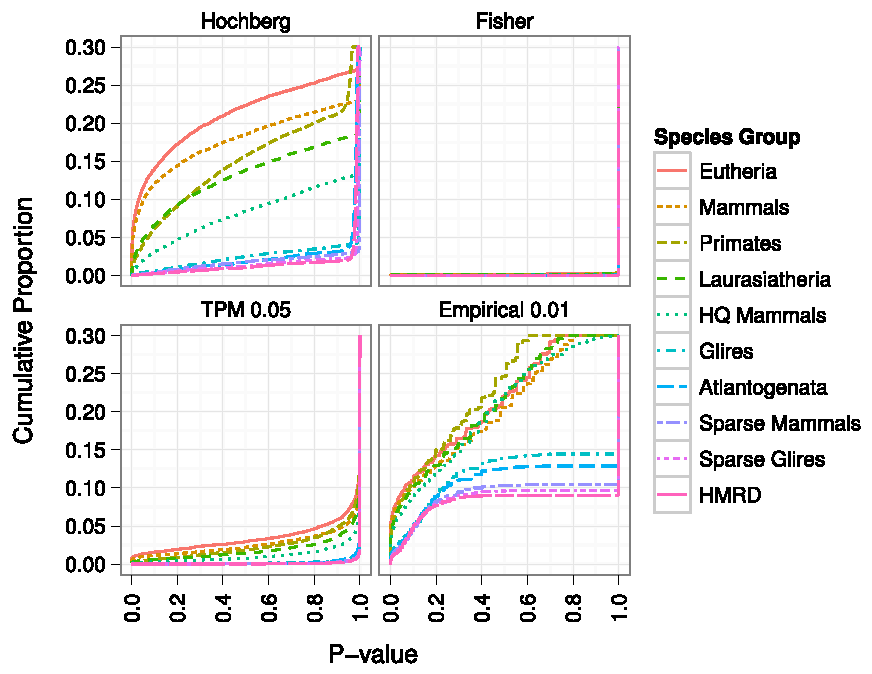
\includegraphics[scale=0.9]{Figs/psg_pvals.pdf}
\caption{Cumulative distributions of gene-wise p-values for positive
  selection resulting from 4 different methods for combining \sw
  estimates within genes. Note that the species groups are listed in
  order of their cumulative proportions at a p-value of 0.5 for the
  Hochberg method. To more clearly show the separation between species
  groups at lower y-values, cumulative proportions above 0.3 are not
  shown.}
\label{fig_psg_pvals}
\end{figure}

The Hochberg and empirical methods both showed much greater
sensitivity and revealed strong differences in the distributions of
p-values between species groups. For the Hochberg method, Eutheria and
Mammals groups showed a large proportion of p-values in the realm of
significance, with roughly 10\% of genes having $p<0.05$. Primates and
Laurasiatheria clustered together with the next highest proportion of
low p-values (roughly 5\% with $p<0.05$), followed by the HQ Mammals
group with roughtly 2\% of genes with $p<0.05$. The other species
groups all showed no visible enrichment for low p-values, with a
largely uniform distribution of p-values in the range of $0<p<1$ and
less than 5\% of genes with a p-value below 1. The empirical method
produced two tight clusters of species groups: the first cluster, with
roughly 5-7\% of genes with $p<0.05$, contained Eutheria, Mammals,
Primates, Laurasiatheria and HQ Mammals; the second cluster, with
roughly 2\% of genes having $p<0.05$, contained the other 5 species
groups. Note that the cumulative curve for species groups in the lower
cluster levels off at around $p=0.2$. This leveling off occurred at
the maximum p-value given to genes with at least one site below the
truncation threshold; the substantial fraction of genes with zero
sites below the truncation threshold yielded p-values near to 1.

The major differences between the Hochberg and empirical methods were
the tighter clustering of the empirical p-values for the 5 species
groups with greater evidence for positive selection and the greater
proportion of low empirical p-values for the 5 species groups with
less evidence for positive selection. Both differences could be
explained by the fact that the Hochberg method assessed significance
based on the absolute magnitude of the \ac{lrt} statistic for positive
selection, while the empirical method assessed significance based on
the magnitude of evidence for positive selection \emph{relative} to
all \sw estimates for a given species group. This had the effect of
increasing the proportion of genes with low p-values for species sets
with less branch length (e.g., Primates, Laurasiatheria, and HQ
Mammals) or less overall evidence for positive selection (e.g., the
five species groups from the lower cluster). As a result, although the
overall pattern for each method was somewhat similar, it appeared that
the empirical method provided greater sensitivity to detect signals of
positive selection while accounting for differences in branch lengths
and the background distribution of \sw selective pressures.

In order to identify a set of confident \acp{psg} for each method it
was important to control for multiple testing across genes, since
several thousand genes were independently tested for positive
selection. This multiple testing issue, resulting from performing many
tests across a genome, was distinct from the previously discussed
issue of multiple testing across \emph{sites} within a gene. In the
case of testing many sites within a gene, the driving question was an
overall hypothesis about the gene (e.g., does the gene contain any
positively-selected sites or not) and the appropriate error rate to
control was the \ac{fwer}. In contrast, the goal of testing many genes
across a genome was not to answer a specific global question (e.g.,
are \emph{any} genes under positive selection), but rather to identify
candidates with a reasonably low number or proportion of likely false
positive results. For this purpose, the \ac{fdr}, defined as the
expected proportion of rejections of the null hypothesis that are
false, is a powerful and easily interpreted type of statistical
control \citep{Benjamini1995}. Thus, the \acp{psg} reported in Table
\ref{table_psg_summary} are those genes which remained significant
after controlling for an expected FDR$<0.1$ using the Benjamini
Hochberg method \citep{Benjamini1995}.

\bbtable
\centering \scriptsize
\begin{tabular}{llrrrrrrrrrrrrr}
\toprule
Filter & Species Group & Genes & \wa & \wg & \psghoch & \psgfisher & \psgtfifty & \psgttwenty & 
\psgtten & \psgtfive & \psgeohfive & \psgeone & \psgefive & \psgeten \\
  \midrule

\input{Tables/psg_summary_default.txt}

  \midrule

\input{Tables/psg_summary_stringent.txt}

  \midrule

\input{Tables/psg_summary_pfam.txt}

\bottomrule
\end{tabular}
\caption{\acp{psg} identified using \sw data with 3 \sw filters, 10
  species groups and different methods to combine p-values across
  sites. The columns \wa and \wg present the arithmetic and geometric
  means, respectively, of the gene-wide \omg values estimated by
  \ac{slr}. To identify \acp{psg}, only genes with at least 50 \sw
  estimates from the given species group and filter were tested. The
  Benjamini-Hochberg method was used to identify \acp{psg} significant
  at FDR$<0.1$ for all methods. Hoch.---Hochberg's method for
  \ac{fwer} control; Fis.---Fisher's combined p-value test;
  TPM---truncated product method using 50\%, 20\%, 10\% and 5\%
  \ac{fpr} thresholds; E---empirical p-values using 0.5\%, 1\%, 5\%
  and 10\% \ac{fpr} thresholds.}
\label{table_psg_summary}
\eetable

Table \ref{table_psg_summary} provides a summary of \acp{psg}
identified by each method for each \sw filter and species group. Only
genes with at least 50 \sw estimates were tested, resulting in
different numbers of genes for different species groups and \sw
filters. Groups containing fewer species, such as Atlantogenata and
HMRD, tended to contain slightly fewer genes than larger groups; this
mirrored differences between species groups in the genome-wide number
of \sw estimates seen in Chapter \ref{ch_mammals1} (see Table
\ref{table_pset_summaries_1}).

The pattern of \ac{psg} counts was qualitatively similar between
different \sw filters, with fewer \acp{psg} found using more stringent
filters. For each combination of species group and method, the
greatest number of \acp{psg} was generally found using the relaxed
filter, fewer were found using the conservative filter, and the fewest
were found using only sites within Pfam domains. This was partially
due to the lower total number of genes retained for analysis with the
two more conservative filters: for the Mammals species group, 15,946
genes contained at least 50 sites for analysis using the default
filter, while the conservative and Pfam filters resulted in only
10,192 and 10,587 genes, respectively. Even after accounting for the
different total gene counts in different filters, the number of
\acp{psg} as a proportion of all genes was still reduced in the more
conservative filters: as an example, for \acp{psg} identified in the
Mammals group using Hochberg \ac{fwer}, 7.8\% of genes were \acp{psg}
using the relaxed filter, 4.7\% using the conservative filter, and
2.8\% using only sites within annotated Pfam domains. A similar trend
was observed for the other \acp{psg} identification methods, showing
that the conservative and Pfam filtered datasets contained
progressively lower proportions of genes subject to positive
selection. This corresponded well with the pattern seen in Chapter
\ref{ch_mammals1} for the prevalence of positively-selected sites.

Comparing between the different methods for identifying \acp{psg}, the
Hochberg \ac{fwer} control and empirical p-value methods were much
more sensitive than the Fisher and \ac{tpm} methods, as expected from
the p-value distributions in Figure \ref{fig_psg_pvals}. The Fisher
method was the most conservative, identifying a vanishingly small
number of \acp{psg} in all species groups. Comparing results from the
\ac{tpm} method at different truncation thresholds, the method provded
to be increasingly more sensitive as the truncation threshold was
decreased; in the Mammals group using the conservative filter, 55
\acp{psg} were identified with a truncation threshold of $p<0.05$. The
empirical method was the least sensitive with a truncation threshold
of $p<0.01$, with increased sensitivity using the lowest threshold
($p<0.005$) and the two higher thresholds ($p<0.05$ and $p<0.1$). The
Hochberg method and the most conservative empirical method yielded 474
and 585 \acp{psg} in the Mammals group, respectively.

Although the Hochberg and empirical methods resulted in similar
numbers of \acp{psg} for the Mammals species group, the empirical
method identified the greater number of \acp{psg} in the smaller
species groups. The pattern of Hochberg \ac{psg} counts across species
groups was reminiscent of the pattern of significant \acp{psc}
identified after controlling the \ac{fdr} (Table
\ref{table_pset_summaries_2}): Mammals and Eutheria yielded several
hundred \acp{psc} and \acp{psg}, Primate and Laurasiatheria yielded a
much smaller but still non-zero number, and the other species groups
yielded none. The consistency of this pattern between \acp{psc} and
\acp{psg} reflected the fact that the Hochberg method for identifying
\acp{psg} was sensitive largely to the existence of any one site
within a gene having a very strong signal of positive selection. Thus,
only the species groups with a large total branch length and a high
prevalence of positive selection produced a large number of Hochberg
\acp{psg}.

In contrast, \acp{psg} from empirical p-values reflected a significant
clustering of less extreme \acp{psc}. As a result, the empirical
method identified some \acp{psg} in species groups where the Hochberg
method identified none. The qualitative pattern between species groups
was largely similar to that seen for the Hochberg \acp{psg}: using the
conservative filter and the empirical method with a truncation
threshold of $p<0.01$, Mammals and Eutheria yielded around 600
\acp{psg}, Primates, Laurasiatheria and HQ Mammals produced around
400, and most other species groups had 50 or fewer \acp{psg}. The
species group with the most striking difference between the Hochbeg
\acp{psg} and the empirical \acp{psg} was the HQ Mammals group, which
had zero Hochberg \acp{psg} but several hundred empirical
\acp{psg}. This was consistent with the intermediate location of the
cumulative curve for HQ Mammals under the Hochberg method in Figure
\ref{fig_psg_pvals}; although this species group showed a greater
enrichment of low p-values than the lowest cluster of curves, it was
not strong enough to produce any significant genes at FDR$<0.1$.

In summary, the 3 types of methods for combining \sw estimates to
identify \acp{psg} showed very different performance patterns across
the different species groups. While the \ac{tpm} and Fisher's method
have been extensively used in large-scale studies, they appeared to
lack power in this application. Control of the \ac{fwer} or the use of
empirical p-values yielded greater numbers of \acp{psg}. Using these
methods to identify \acp{psg}, the 10 species groups fell into 2
clusters, each with a very different proportion of identified
\acp{psg}.

\subsection{Overlaps between positively-selected genes in different species groups}

\begin{figure}
\centering
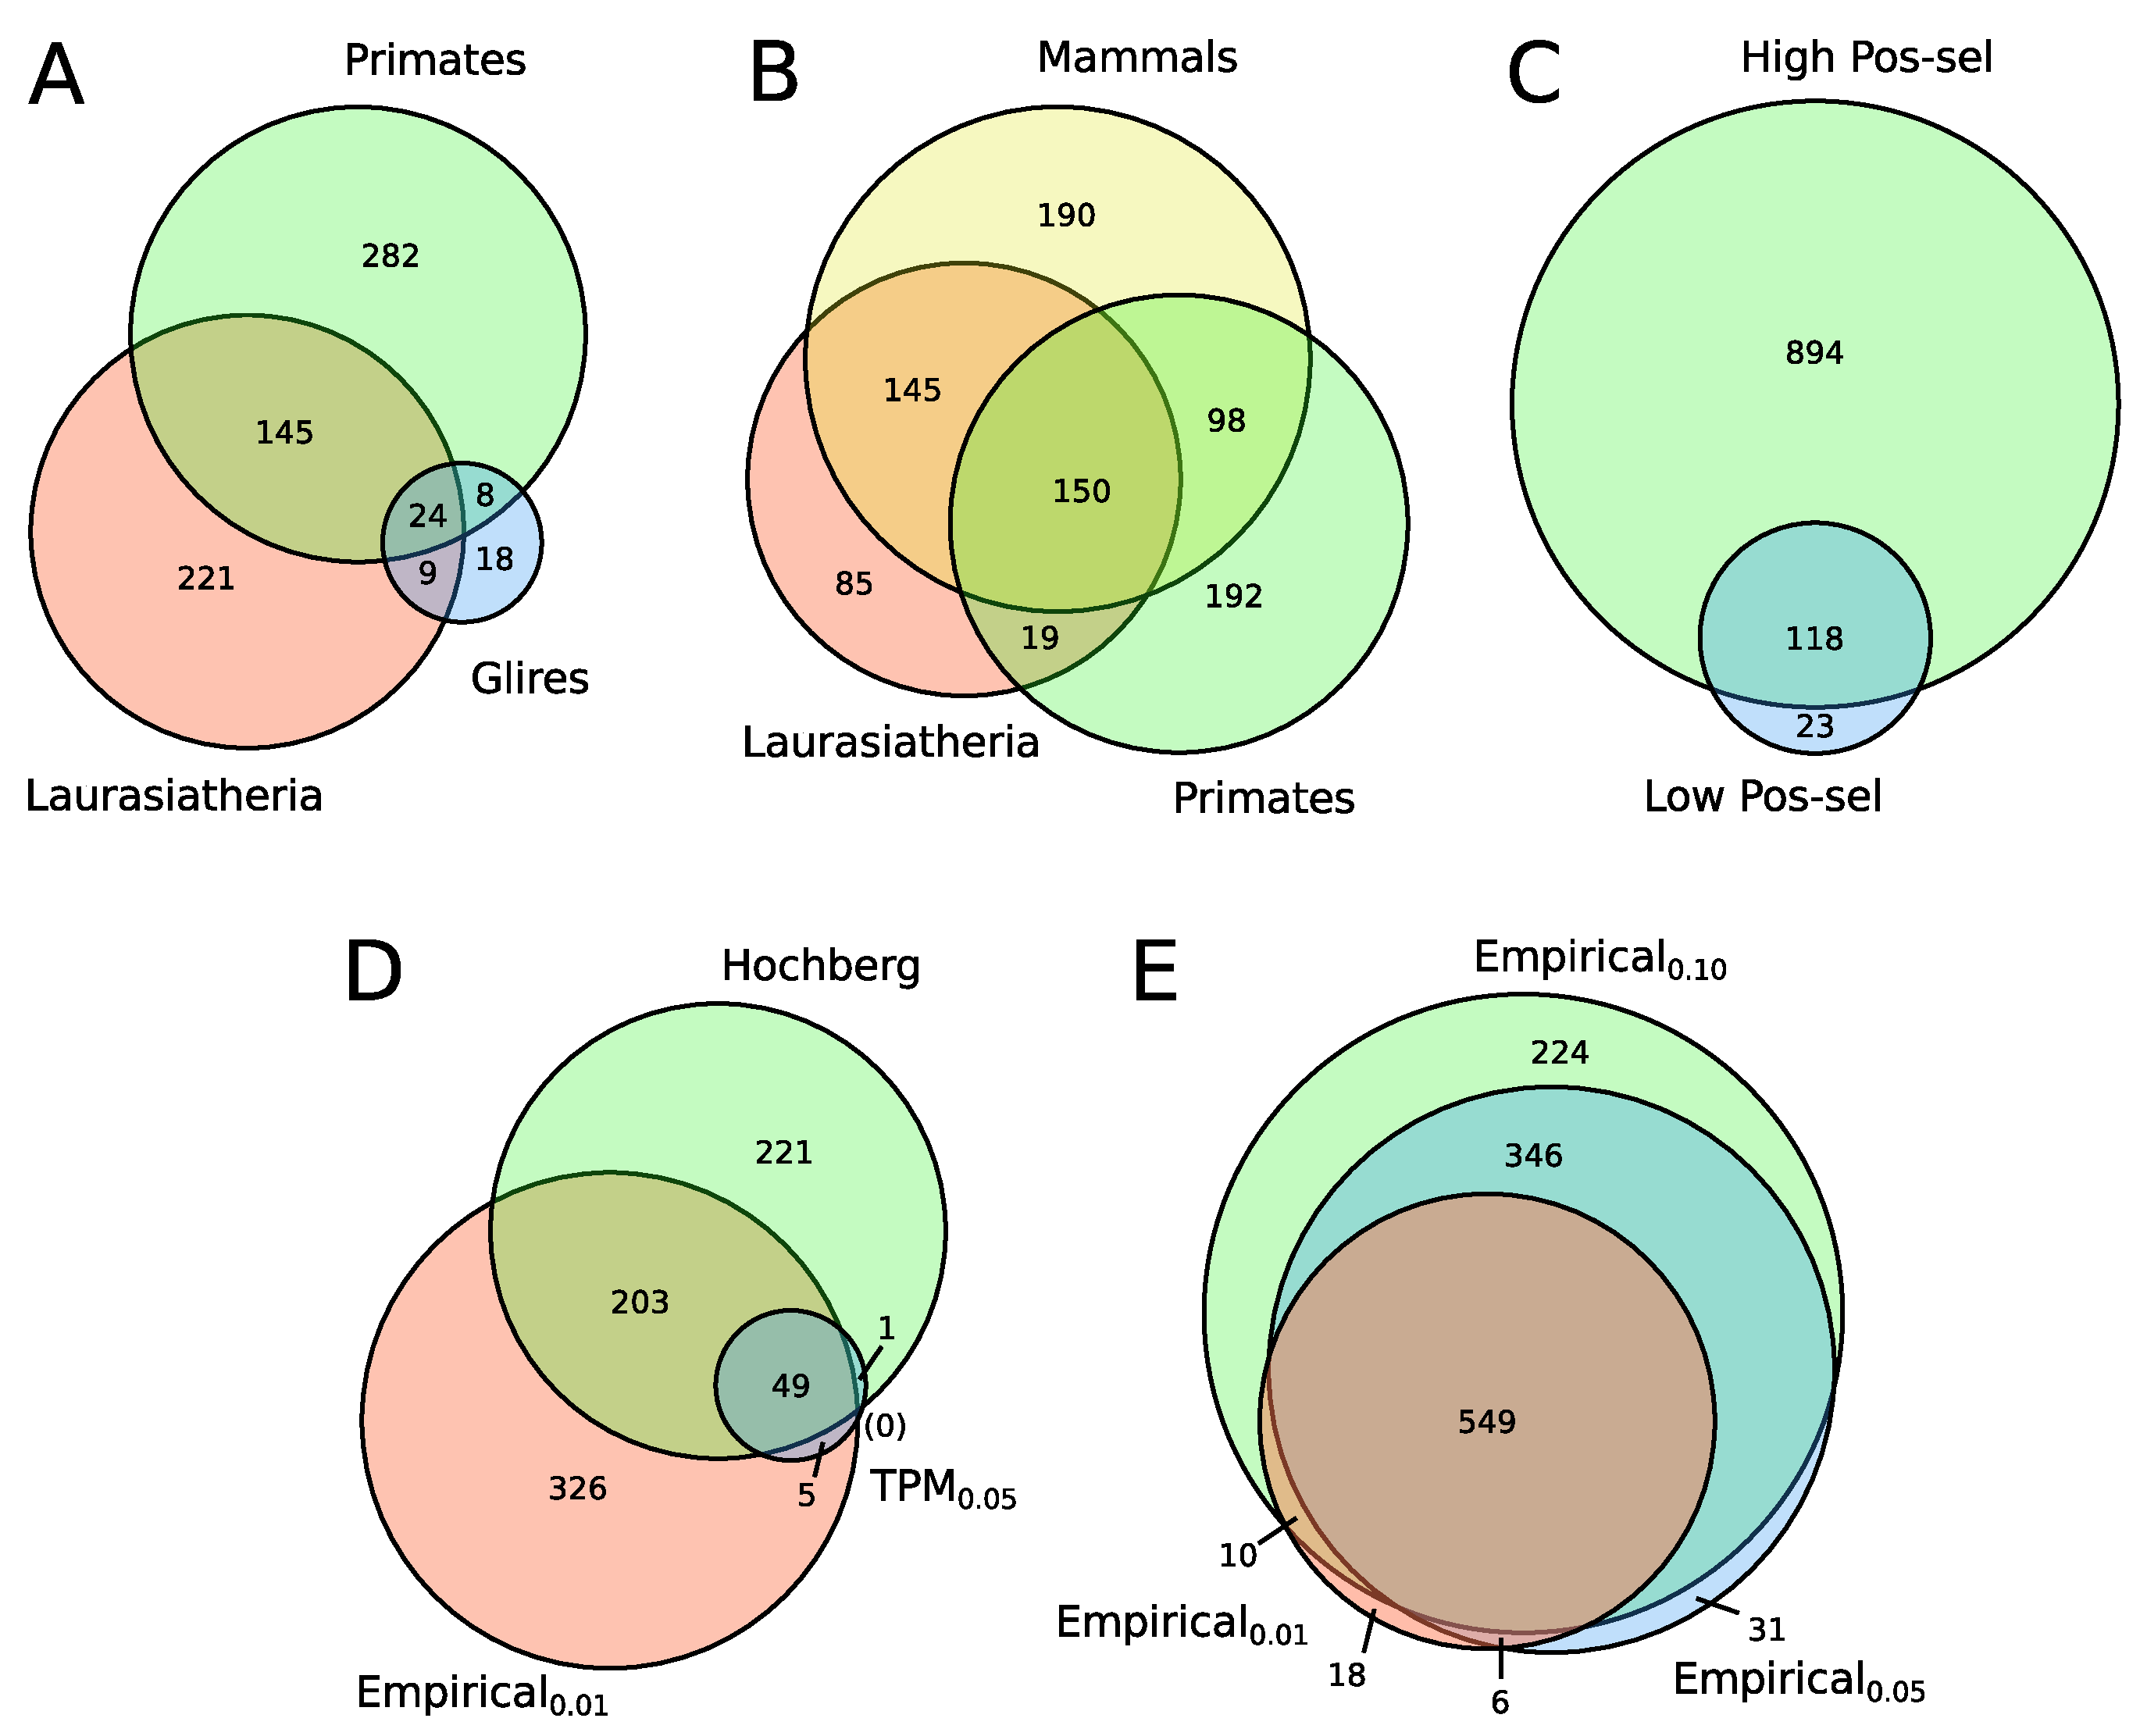
\includegraphics[scale=0.3]{Figs/psg_venns.pdf}
\caption{Venn diagrams of \acp{psg} identified in different species
  groups and using different methods. (A) \acp{psg} identified using
  empirical p-values in Primates, Glires, and Laurasiatheria. (B)
  \acp{psg} identified using empirical p-values in
  Mammals. Laurasiatheria and Primates. (C) \acp{psg} identified using
  empirical p-values in species groups with high and low levels of
  positive selection. (D) \acp{psg} identified in the Mammals group
  using three different methods for combining \sw estimates within
  genes. (E) \acp{psg} identified in the Mammals group using the
  empirical p-value method with 3 different truncation thresholds:
  $p<0.01$ (smallest circle, left), $p<0.05$ (middle circle, right),
  $p<0.10$ (largest circle, top).}
\label{fig_psg_venns}
\end{figure}

Using the sets of significant \acp{psg} from Table
\ref{table_psg_summary}, it was possible to identify how many
\acp{psg} were shared between, or unique to, different species groups
or methods. Unless otherwise specified, all future analyses in this
chapter will be derived from the conservatively-filtered dataset.

I first looked at the distribution of \acp{psg} from the empirical
method with a $p<0.01$ truncation threshold across species
groups. Overall, a total of 1035 out of 11520 genes, or 8.9\% of those
investiated, were identified as a \ac{psg} in at least one of the
species groups. Figure \ref{fig_psg_venns} shows a more detailed
breakdown of how many \acp{psg} were shared between various species
groups. Figure \ref{fig_psg_venns}A compares genes from the three
major mammalian superorders, showing that Primates and Laurasiatheria
share roughly a third of their \acp{psg} and that around two-thirds of
\acp{psg} in Glires are also significant in Primates, Glires, or
both. Figure \ref{fig_psg_venns}B looked at \acp{psg} shared between
Primates, Laurasiatheria, and Mammals (which contained all of the
species within the Primates and Laurasiatheria groups), showing
roughly equal mixtures of shared and unique genes. Finally, I split
the 10 species groups into 2 clusters based on the prevalence of
\acp{psg}: Mammals, HQ Mammals, Eutheria, Primates and Eutheria were
considered ``High Pos-sel'' groups, and the rest were considered ``Low
Pos-sel'' groups. Figure \ref{fig_psg_venns}C shows the overlap
between the union of \acp{psg} identified in each group; \acp{psg}
from the High Pos-sel cluster of species groups is largely a superset
of those from the Low Pos-sel cluster, with only 23 \acp{psg} unique
to the species groups which showed less overall positive selection.

Expanding the count to include \acp{psg} identified by the Hochberg,
Fisher, and truncated product methods (at a truncation threshold of
$p<0.05$), the total number of \acp{psg} identified was 1300, or
11.3\% of all genes tested. Compared to the 1035 from the empirical
method alone, the additional 265 genes came from the Hochberg method
in the Eutheria and Mammals groups. Figure \ref{fig_psg_venns}D shows
the overlap of \acp{psg} identified in the Mammals group by different
methods; while the \ac{tpm} yielded no unique \acp{psg}, a large
number of the Hochberg genes were unique, indicating that the Hochberg
and empirical p-value methods were sensitive to different patterns of
positively-selected sites within genes. In contrast, Figure
\ref{fig_psg_venns}E shows that the different variants of the
empirical method using different truncation thresholds yielded largely
the same set of \acp{psg}, but with increasing sensitivity as the
truncation threshold was relaxed from $p<0.01$ to $p<0.10$.

\section{Functional analysis of \acp{psg} and comparison to previous studies}

I used \ac{go} term annotations from the \ens database to identify
functional categories enriched for \acp{psg}. \ac{go} annotations for
all human genes were downloaded from version 64 of \ens and were
applied to the mammalian alignment containing each human gene. As the
\ac{go} ontology contains links between terms forming a directed
acyclic graph, I followed the common practice of applying the set of
all ancestral, and thus less-specific, terms to each gene as well
\citep{Rivals2007}. Only terms within the Biological Process ontology
were included in this analysis, as the Molecular Function and Cellular
Component hierarchies contain less information on the types of
processes generally associated with the presence of positive selection
in mammalian genes \citep{Macaque2007}.

Two methods were employed to identify \ac{go} terms enriched for
\acp{psg}. First, a simple test for independent association was
performed for each term: a 2x2 contingency table was filled with the
counts of \acp{psg} and non-\acp{psg} which were annotated and not
annotated with the current term (each combination of which filled one
cell of the table), and \ac{fet} was used to perform a one-sided test
for independence of rows and columns. A highly significant \ac{fet}
p-value thus represented strong evidence for a positive association
between a gene being positively-selected and being annotated with the
given term \citep{Rivals2007}. To control for multiple tests being
performed, I excluded all terms containing fewer than 5 \acp{psg} (to
reduce the number of tests performed and to avoid including highly
specific and less biologically-informative \ac{go} terms) and used the
Benjamini-Hochberg method to identify the \ac{fet} p-value needed to
control for an expected \ac{fdr}$<0.1$ within each set of
\acp{psg}. The second method I used to assess significance was the
\texttt{weight} algorithm from the \topgo program
\citep{Alexa2006a}. The \texttt{weight} algorithm also uses \ac{fet}
to identify significant associations between terms and genes of
interest, but it accounts for the fact that gene annotations for
nearby terms in the \ac{go} graph structure are highly correlated by
reducing the significance of terms which have more specific,
significantly-enriched descendant terms. The result of this weighting
is that clusters of closely-related and highly significant terms,
which may otherwise clutter the list of top \ac{fet} results with an
uninformative set of very similar terms, are thinned out by reducing
the p-values of the less-specific ancestors. Only terms which were
significant by both \ac{fet} (FDR$<0.1$) and the \texttt{weight}
algorithm ($p<0.1$) were included in the top and bottom sections of
Table \ref{table_go}. Terms with more than 300 or fewer than 30
annotated genes were also excluded from inclusion in the top or bottom
sections of Table \ref{table_go} for clarity.

These two methods were applied to several sets of \acp{psg} in order
to assess the consistency of enriched terms between different methods
for identifying \acp{psg} and different species groups. The
conservatively-filtered dataset was used for all tests. Each set of
enriched terms was assigned a letter for identification in Table
\ref{table_go}; those letters are included here in parentheses for
reference. From the Mammals group, I tested for enriched \ac{go} terms
in the 474 \psghoch \acp{psg} (\texttt{H}), the 585 \psgeone \acp{psg}
(\texttt{M}), the 934 \psgefive \acp{psg} (\texttt{m}), and the 202
genes in the top 2\% genome-wide by overall \dnds value
(\texttt{D}). The latter group was defined using gene-wide \dnds
values output by \ac{slr}, based on fitting a M0-like codon model to
the mammalian alignment. To evaluate \acp{psg} identified in the
mammalian superorders, I tested the 459 \psgeone \acp{psg} from
Primates (\texttt{P}), the 409 \psgefive \acp{psg} from Glires
(\texttt{g}), and the 400 \psgeone \acp{psg} from Laurasiatheria
(\texttt{L}). Finally, the set of 273 genes with independent evidence
for positive selection in each of the Primates, Glires, and
Laurasiatheria groups was obtained by taking the least significant
\psgefive p-value for each gene from each species group and
identifying genes which remained significant (\texttt{i}). Note that
groups indicated by lowercase letters correspond to those using the
less conservative \psgefive \ac{psg} definition.

In order to facilitate a comparison with functional associations
reported in previously-published studies, I also collected the lists
of terms enriched for \acp{psg} from Clark et
al. \citeyearpar{Clark2003} (\texttt{C}), the Rhesus Macaque Genome
Sequencing and Analysis Consortium \citeyearpar{Macaque2007}
(\texttt{R}), and Kosiol et al. \citeyearpar{Kosiol2008} (\texttt{K}).

\bbtable
\centering \scriptsize
\begin{tabular}{llllrrrrrl}
\toprule

\multicolumn{2}{c}{\ac{go} Term} & \multicolumn{2}{c}{Enriched in} & \multicolumn{6}{c}{Values for Mammals \psgefive (label \texttt{M} in ``This Study'' column)} \\

\cmidrule(r){1-2}
\cmidrule(r){3-4}
\cmidrule(r){5-10}

ID & Description & \multicolumn{1}{c}{This Study} & \multicolumn{1}{c}{Lit.} & \ac{fet} & \topgo & Ann.  & Sig. & Exp. & Top 5 Genes \\

\midrule
\multicolumn{4}{l}{Top 10 Enriched Terms} & & & & & & \\
\midrule

\input{Tables/psg_go_top.txt}

\midrule
\multicolumn{4}{l}{Other Terms Commonly Identified in the Literature} & & & & & & \\
\midrule

\input{Tables/psg_go_them.txt}

\midrule
\multicolumn{4}{l}{Other Terms Identified in This Study but Not in
  the Literature} & & & & & & \\ \midrule

\input{Tables/psg_go_me.txt}


\bottomrule
\end{tabular}
\caption{Example \ac{go} terms enriched for \acp{psg} in this study
  and in the literature. Top section: the 10 terms most significantly
  enriched for \psgefive \acp{psg} in the Mammals species
  group. Middle section: other terms found in at least 2 of 3
  published genome-wide scans. Bottom section: other terms enriched
  for \acp{psg} in this study but not in the literature. The presence
  or absence of characters under the columns ``This Study'' and
  ``Lit.'' indicates which sets of genes from this or
  previously-published studies showed enrichment for \acp{psg} for
  that term (see text for definitions). The last 6 columns show values
  from the Mammals \psgefive set, corresponding to the `\texttt{M}'
  flag; bold P-values indicate significance (FDR$<0.1$ for \ac{fet}
  and p$<0.05$ for \topgo). Genes discussed in the text are presented
  in bold face. Lit.---literature; \ac{fet}---Fisher's Exact Test;
  Sig.---Significant; Exp.---Expected.}
\label{table_go}
\eetable

Table \ref{table_go} summarizes the results of the \ac{go} term
enrichment tests, showing for three sets of terms which groups of
genes from this study, and which previously-published studies,
identified a significant enrichment of \acp{psg}.

The top section shows 10 of the \ac{go} terms most strongly enriched
for Mammalian \psgefive \acp{psg} according to \ac{fet}. The top few
terms, including \emph{inflammatory response}, \emph{innate immune
  response}, \emph{defense response to virus} and \emph{defense
  response to bacterium}, represented genes involved in host defense
and immune response---two of the functions most commonly associated
with positive selection in mammals \citep{Nielsen2005b}. Accordingly,
the top four terms were identified in one or two previously-published
studies and in most or all of the species groups and \acp{psg}
identification methods evluated in this study. Interestingly, the term
\emph{mitotic prometaphase} was associated with \acp{psg} in almost
all gene sets from this study, but it was not found by any of the sets
of enriched terms from the literature. The next several terms, most of
which were not found in the literature, showed a more mixed pattern of
enrichment across gene sets from this study. Some of these terms,
including \emph{mitosis} and \emph{centrosome organization} were
connected to the more strongly-enriched \emph{mitotic prometaphase}
term and showed many of the same significant genes; others, such as
\emph{platelet degranulation} and \emph{leukocyte migration} were
distinct in function and composition of Mammalian \psgefive \acp{psg}.

The middle section of Table \ref{table_go} focuses on \ac{go} terms
commonly associated with \acp{psg} in the literature which were not
included in the 10 top terms, showing all terms identified in at least
2 of the 3 previously published studies. The first 5 terms largely
recapitulated those included in the top section relating to defense
response and inflammation, all of which were identified in most gene
sets from the current study. The next several terms, including
\emph{sensory perception of taste} and \emph{cell surface receptor
  linked signaling}, were more related to sensory perception and were
uniformly not associated with \acp{psg} in this study. The lack of an
association for these terms in the current study was surprising, as
olfaction and sensory perception have been among the most consistently
identified functional categories in large-scale scans for positive
selection \citep{Nielsen2005,Nielsen2005b}. One explanation for this
difference may be that the removal of highly-duplicated genes from the
conservatively-filtered dataset has reduced the number of olfactory
and sensory genes available for analysis. While there was some
evidence that the current dataset was depleted of olfactory genes
compared to previous analyses (according to Table \ref{table_go} only
17 genes were annotated with \emph{sensory perception of smell}, while
Kosiol et al. \citeyearpar{2008} analyzed 229 such genes), the number
of genes annotated with \emph{sensory perception} (274) and
\emph{sensory perception of chemical stimulus} (36) were still large
enough to produce a significant enrichment if one existed. Other
possible explanations included the possibility that
positively-selected sensory genes were more prone to exclusion from
the current analysis for other reasons (for example, if their
alignments contained more clustered \nsyn substitutions) or less
sensitivity in the current study to the patterns of positive selection
occurring in sensory perception genes.

The bottom section of Table \ref{table_go} shows the remainder of
terms which were identified in the current study, but not in previous
studies providing \ac{go} term enrichments, as associated with
\acp{psg}. The first term, \emph{double-stranded break repair}, was
identified in 3 of the 8 gene sets, with the association with
\acp{psg} driven by genes such as \gene{SETX}, a RNA helicase which
causes ataxia and lateral sclerosis when defective
\citep{Suraweera2007}, and \gene{BRCA2}, a tumor suppressor gene for
which a common allele is associated with an increased risk of breast
cancer and whose close relative, \gene{BRCA1}, has been shown to be
positively selected in mammals \citep{Huttley2000a}. Some of the next
terms, including \emph{cell division} and \emph{T cell costimulation}
and \emph{TNF superfamily cytokine production}, were similar to other
terms in the first two sections and contained similar sets of
\acp{psg}, but the terms \emph{organic anion transport} and
\emph{spermatogenesis} were quite distinct in their function and set
of associated \acp{psg}. The anion transport term contained largely
members of the \ac{slc} gene superfamily, a 300-strong group of
membrane-bound transporter genes \citep{He2009}, while the
\emph{spermatogenesis} category has been widely reported in other
studies of mammalian positive selection not included in Table
\ref{table_go}
\citep{Torgerson2002,Swanson2003,Clark2005,Nielsen2005}.

The \ac{go} term enrichments indicated a strong prevalence of positive
selection in genes related to core cellular processes such as cell
division and DNA repair. Many of these associations were noted and
discussed by Nielsen et al. \citeyearpar{Nielsen2005}, who
hypothesized an interesting connection between \acp{psg} and
cancer-related genes in these functional categories. Nielsen et al.
suggested that cancer-related genes, which are often involved in cell
proliferation and apoptosis pathways, may be likely targets of
positive selection resulting from genetic conflict due to their
involvement in processes known to lead to positive selection, such as
the proliferation of immune cells \citep{Sawyer2005a} or sperm
competition \citep{Torgerson2002,Clark2005}. This hypothesis was
developed and expanded by Crespi and Summers \citeyearpar{Crespi2006},
who analyzed the results of several scans for positively-selected
genes through the lens of cancer risk. Crespi and Summers argued that
positive selection resulting from ``antagonistic coevolution'' between
various entities (e.g., hosts and parasites, parents and offspring, or
sperm cells and eggs) has been the driving force behind the evolution
of increased cancer risk. Although similar trends were observed by
Nielsen et al., the current study provided additional support for an
association between positive selection and cancer-related genes,
expanding the list of \acp{psg} in functional categories related to
cancer progression and containing known tumor suppressor genes.

A more surprising result from the \ac{go} term analysis was the strong
enrichment of \acp{psg} in terms related to mitosis and chromosome
segregation. None of these terms were identified in the previous
studies analyzed, but I found strong enrichments for terms such as
\emph{mitosis}, \emph{centrosome organization}, and \emph{chromosome
  segregation}. All of these terms were identified as enriched for
\psgeone \acp{psg} in Mammals, while \emph{centrosome organization}
was enriched for \psgeone in Laurasiatheria and for \psgefive in
Glires. Among the top \acp{psg} within these terms were \gene{HAUS6},
a member of the HAUS microtubule-binding complex which is vital to the
mitotic spindle assembly and maintenance of the centrosome,
centrosomal proteins \gene{CEP152} and \gene{CEP250}, and several
centromere proteins including \gene{CENPT}, \gene{CENPI},
\gene{CENPQ}, and \gene{CENPH}. There has been great interest
surrounding the evolution of centromeric DNA and proteins ever since
Henikoff, Ahmad and Malik proposed the ``centromere paradox''
\citeyearpar{Henikoff2001}. Based on the observation that both
centromeric DNA and centromere-related proteins were rapidly evolving
in animals, the authors postulated an ongoing genetic conflict between
centromeric DNA and proteins resulting from the unequal transmission
of chromosomes during female meiosis
\citep{Henikoff2001,Malik2002,Malik2009}. Initial comparative analysis
of the major centromeric protein \gene{CENPA} gene showed it to be
positively-selected in \emph{Drosophila} and \emph{Arabidopsis} but
not in mammals, while a more recent study in primates identified
positively-selected residues in \gene{CENPA} and three other
centromeric proteins \citep{Schueler2010}. The current identification
of several positively-selected centromere proteins provided
large-scale corroboration of the result from primates, showing that
positive selection in centrosomal and centromeric proteins is a major
component of the overall set of \acp{psg} throughout mammals. In all,
12 out of the 17 centromeric proteins included in this analysis showed
evidence of positive selection in either the relaxed or
conservatively-filtered datasets.

\section{Comparing \acp{psg} identified by different studies}

Somewhat surprisingly, no direct comparison between \acp{psg}
identified in large-scale scans for positive selection has been
published, despite the observation that many similar terms and genes
tend to occur in studies including different species and using
different methods \citep{Nielsen2005,Kosiol2008}. To gain a better
understanding of the amount of similarity between the results from
this analysis and from previously-published studies, I performed a
gene-by-gene comparison with the sets of \acp{psg} described by Clark
et al. \citeyearpar{Clark2003}, Nielsen et
al. \citeyearpar{Nielsen2005}, the Rhesus Macaque Genome Sequencing
and Analysis Consortium \citeyearpar{Macaque2007}, and Kosiol et
al. \citeyearpar{Kosiol2008}. The goals of this analyses were
conceptually similar to those of the previous section: to identify
trends in shared and unique signatures of positive selection from this
and previous genome-wide scans.

I first mapped the sets of genes described by each of the above
studies to the set of genes included in this analysis using the
supplementary data tables provided alongside each publication. The
process was slightly different for each study due to the different
formats provided.

Clark et al. \citeyearpar{Clark2003} provided NCBI RefSeq gene IDs,
which I converted to Ensembl gene IDs using index files downloaded
from the NCBI Entrez gene database \citep{Maglott2005}; this resulted
in 5,636 of the original 6,145 genes being successfully
mapped. Following Clark et al. \citeyearpar{Clark2003}, genes with
$p<0.01$ for the M2 test in either the human or chimpanzee branch were
taken as \acp{psg}, yielding 272 successfully mapped
\acp{psg}. Nielsen et al. \citeyearpar{Nielsen2005} provided a table
including Ensembl gene IDs, NCBI RefSeq gene IDs, and gene names for
each of the 20,362 genes included in their study. I used all three
pieces of information to attempt to match those genes to the current
dataset, but only 11,402 of the original genes were successfully
matched. Still, these genes appeared to contain most of the 50 top
\acp{pst} reported in their analysis \citep{Nielsen2005}. Although the
authors did not provide specific criteria by which \acp{psg} were
defined, I took the lowest \ac{lrt} value from the 50 genes described,
1.67, and identified 142 successfully mapped genes with \ac{lrt}
values greater than that value. The Rhesus Genome Sequencing and
Analysis Consortium \citeyearpar{Macaque2007} provided the names of
179 \acp{psg} identified using a branch-site test along any branch of
the primate tree. Of those, 123 genes were matched by name to genes
included in the current study. Finally, Kosiol et
al. \citeyearpar{Kosiol2008} provided a UCSC browser track with
chromosomal coordinates and scores based on a test across the entire
mammalian phylogeny for 16,529 genes, of which 544 were
positively-selected at FDR$<0.1$. Using chromosomal coordinates to
match genes in the current dataset, 14,460 genes and 395 \acp{psg}
were identified.

\begin{figure}
\centering
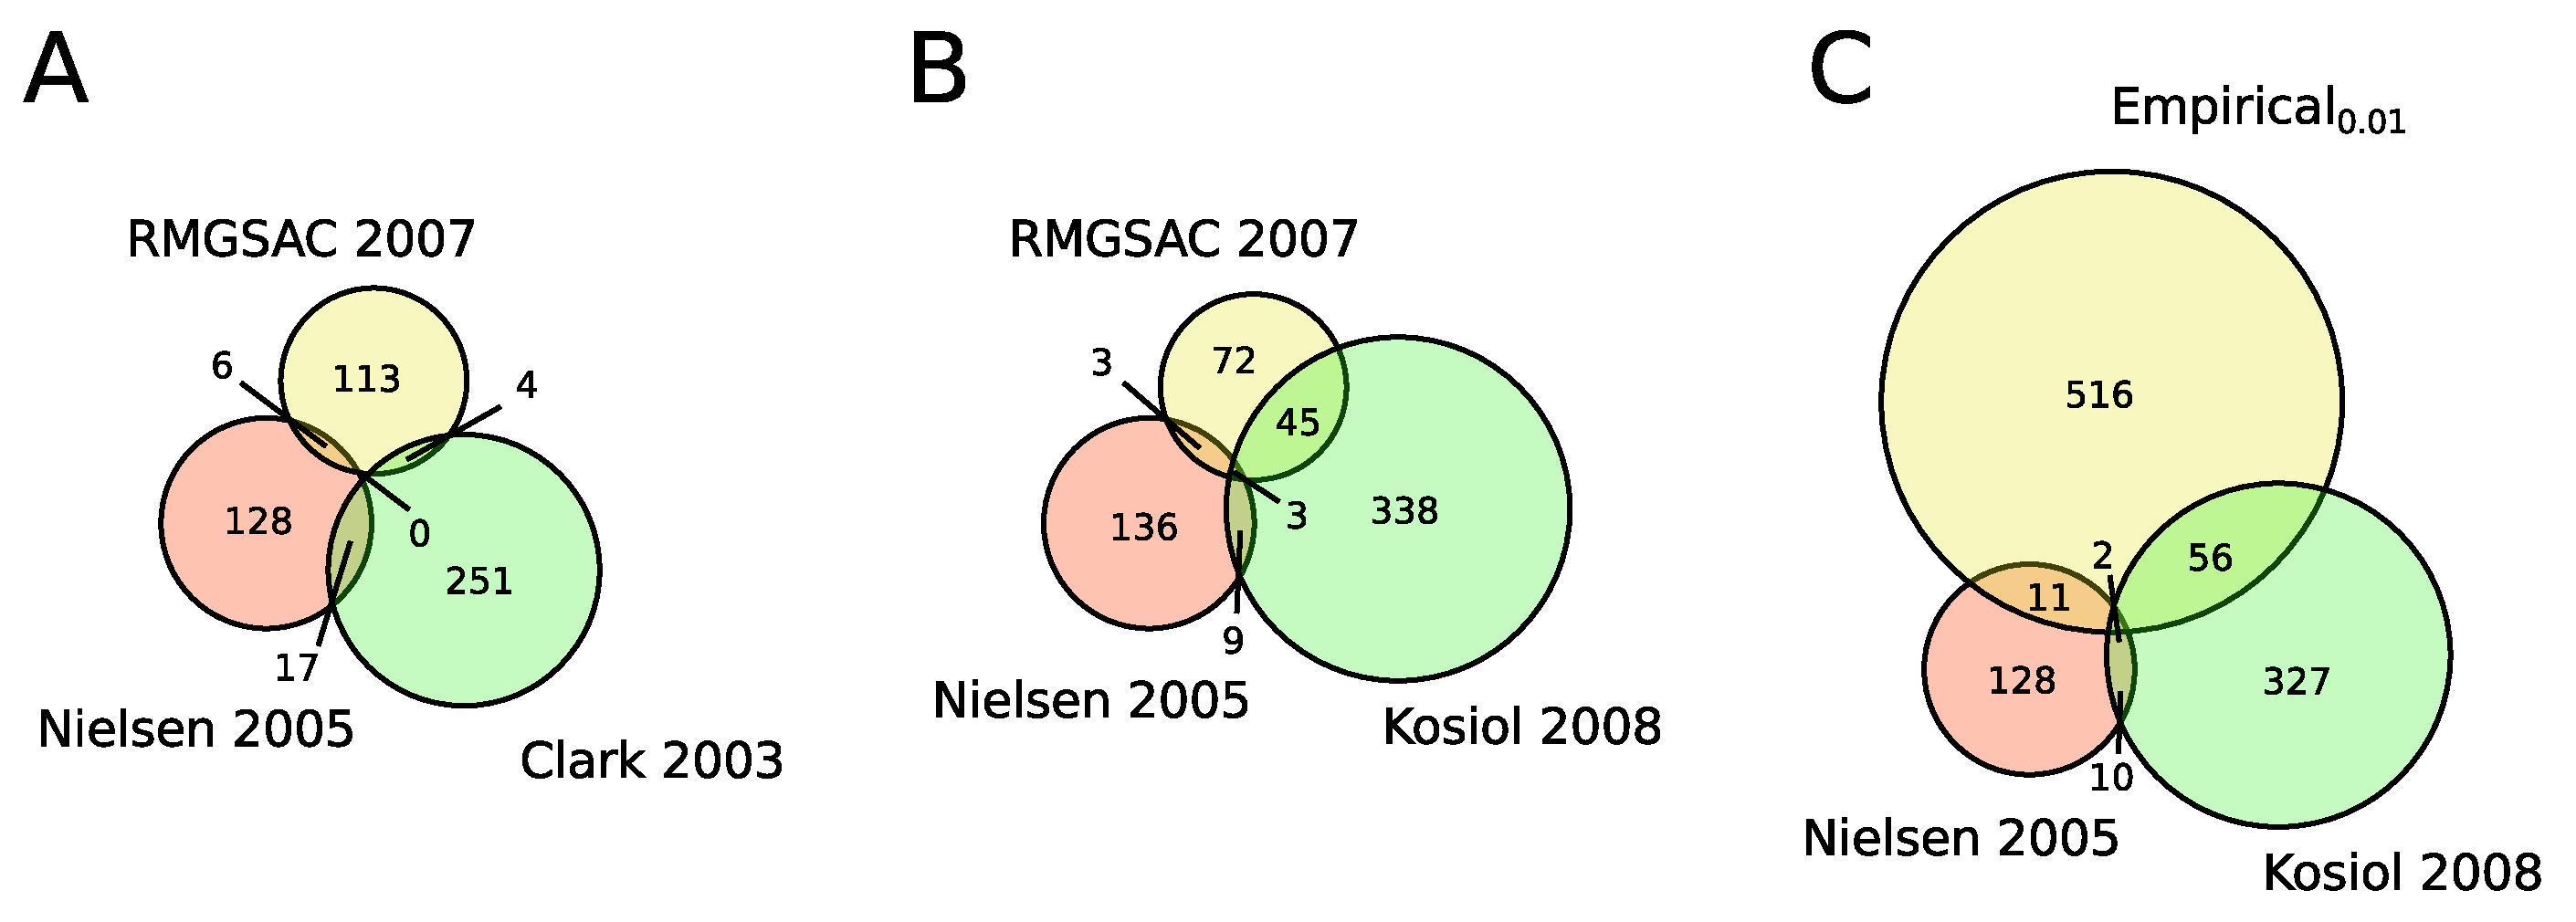
\includegraphics[scale=0.3]{Figs/pub_psg_venn.pdf}
\caption{Venn diagrams of \acp{psg} identified in different
  studies. (A) \acp{psg} identified in primates by Clark et
  al. \citeyearpar{Clark2003}, Nielsen et
  al. \citeyearpar{Nielsen2005} and the Rhesus Macaque Genome
  Sequencing and Analysis Consortium \citeyearpar{Macaque2007}. (B)
  \acp{psg} identified in primates and mammals by Nielsen et
  al. \citeyearpar{Nielsen2005}, the Rhesus Macaque Genome Sequencing
  and Anaalysis Consortium \citeyearpar{Macaque2007} and Kosiol et
  al. \citeyearpar{Kosiol2008}. (C) \acp{psg} identified in primates
  and mammals by Nielsen et al. \citeyearpar{Nielsen2005}, Kosiol et
  al. \citeyearpar{Kosiol2008} and this study using the Mammals
  species group, conservative filter, and the \psgeone method.}
\label{fig_pub_psg_venn}
\end{figure}

Figure \ref{fig_pub_psg_venn} shows the overlap between \acp{psg}
identified in this and previously-published studies. Note that the
total numbers of \acp{psg} are smaller than those noted in the
previous paragraph, as genes which were absent from the
conservatively-filtered dataset were removed. (Results from a
comparison using the relaxed filter were qualitatively similar to
those in Figure \ref{fig_pub_psg_venn}.) Overall, the lack of overlap
in identified \acp{psg} was striking: Figure \ref{fig_pub_psg_venn}A
shows the overlap between the three studies in primates, with zero
genes shared by all 3 studies and from 4 to 17 genes shared between
any pair. Although each analyses identified similar numbers of
\acp{psg}, very few of the actual genes identified were in
common. This result did not appear to be an artifact of genes lost
during the mapping process, as Nielsen et al. also noted that only 1
of their top 50 genes was also identified by Clark et
al. \citeyearpar{2003} as evolving under positive selection. Figure
\ref{fig_pub_psg_venn}B shows slightly more overlap between the two
most recent studies, with 45 \acp{psg} shared between Kosiol et
al. and the Rhesus genome analysis. The comparison between \acp{psg}
from Nielsen et al., Kosiol et al., and the set of \psgeone \acp{psg}
from the Mammals species group shown in Figure \ref{fig_pub_psg_venn}C
revealed a similar number of overlapping genes, despite the larger
overall number of \acp{psg} identified in the current study.

The comparison of overlapping \acp{psg} was somewhat limited, as it
required the use of a cutoff threshold to identify each set of
\acp{psg} and did not easily allow for a comparison between the
different methods. For example, although Figure
\ref{fig_pub_psg_venn}C showed a greater number of overlapping genes
between Kosiol et al. and the current study than between Nielsen et
al. and the current study (154 vs. 31), it was unclear whether this
was due to the greater overall number of \acp{psg} identified by
Kosiol et al., or to a greater tendency for this study and Kosiol et
al. to identify common \acp{psg}. By eye, it seemed as if both Kosiol
et al. and Nielsen et al. shared a similar proportion of \acp{psg}
with the current study.

As an alternative approach to comparing between the current results
and previous studies, I constructed a series of \ac{roc} curves for
each published study. For each study, the set of \acp{psg} was used as
the binary classifier (or ``truth'' value), and a set of 4 gene-wide
$p$-values or \dnds estimates from the current study were evaluated as
test statistics. Curves were constructed by sorting the list of
matched genes by each test statistic and counting the cumulative
number of \acp{psg} identified as the test statistic increased in
value. To test whether the choice of species group affected the
proportion of shared \acp{psg}, I included gene-wide \dnds estimates
for Primates and Mammals (where the test statistic was the negative
\dnds value, so the genes with highest \dnds were sorted first), and
to test whether the method used to combine \sw estimates within genes
had an effect, I included \psgeone and \psghoch $p$-values as test
statistics.

\begin{figure}
\centering
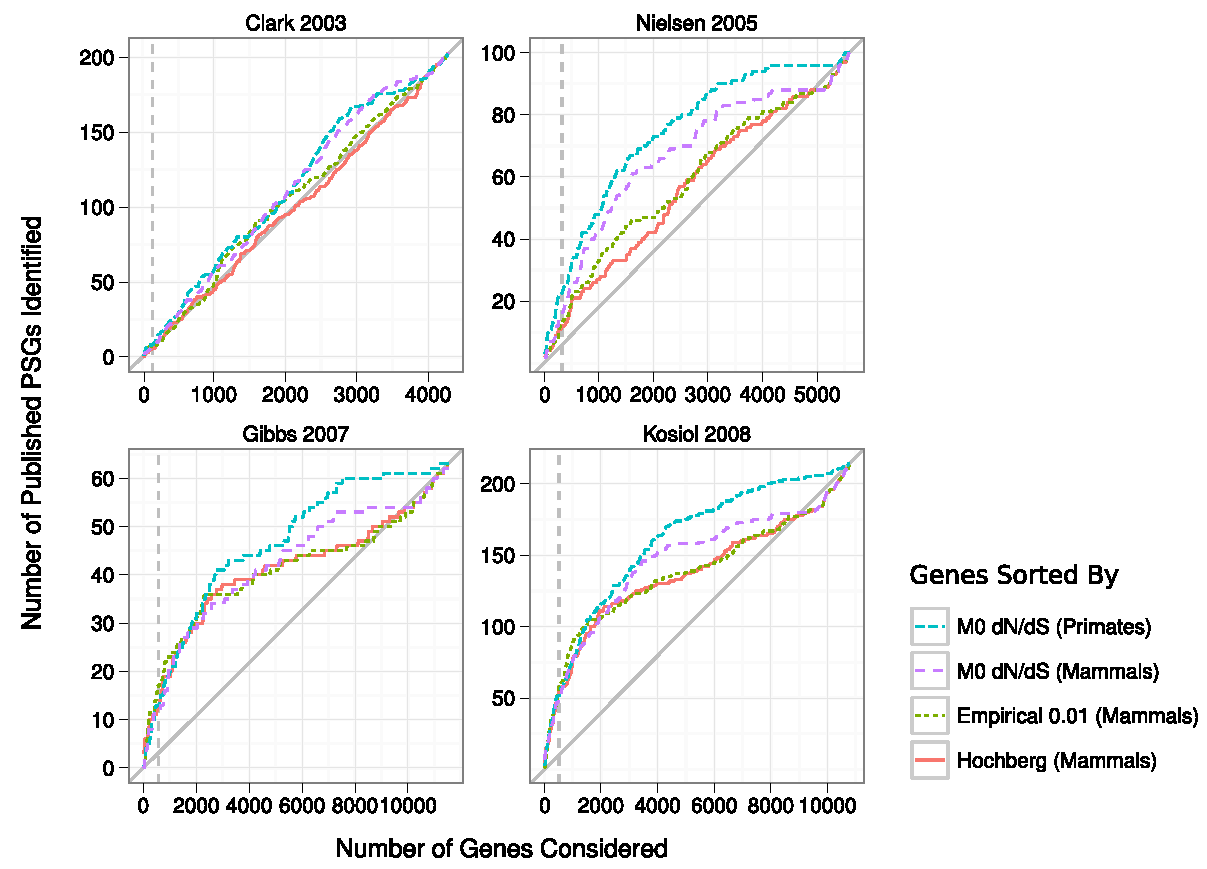
\includegraphics[scale=0.78]{Figs/psg_rocs.pdf}
\caption{\ac{roc} curves for using \dnds estimates and different
  \ac{psg} identification methods to identify \acp{psg} in
  previously-published studies. Within each panel, the x-axis
  represents all genes successfully matched between the published
  study and the current analysis and the y-axis represents the number
  of \acp{psg} within the matching genes. Each curve traces the
  cumulative number of \acp{psg} identified in the published study
  when the top $N$ genes, according to the test statistic, were
  considered. A dashed vertical line is drawn on each panel at the
  x-axis value corresponding to the number of \psgeone \acp{psg} in
  the Mammals species group.}
\label{fig_psg_rocs}
\end{figure}

Figure \ref{fig_psg_rocs} shows the \ac{roc} curves comparing the
current dataset to each of the four previously published studies. The
vertical dashed lines correspond to the FDR$<0.1$ threshold of the
\psgeone $p$-values in Mammals, making the intersection of the
\psgeone \ac{roc} curve at the vertical lines equivalent to the
numbers of overlapping \acp{psg} seen in Figure
\ref{fig_pub_psg_venn}C for the Nielsen et
al. \citeyearpar{Nielsen2005} and Kosiol et
al. \citeyearpar{Kosiol2008} sets of \acp{psg}.

The Clark et al. \citeyearpar{Clark2003} curves hardly strayed from
the diagonal line, showing little ability beyond random chance to
identify \acp{psg} from that study. This was not necessarily
unexpected, as that study tested for positive selection only along the
very short human and chimpanzee branches of the primate tree, while
even the Primates species group from the current study contained
sequences from species as distant as tarsier, covering much more
branch length and a much more diverse set of primate species. The
Nielsen et al. \citeyearpar{Nielsen2005} study showed a noticeably
stronger enrichment for \acp{psg} in genes with low $p$-values or high
\dnds values in the current study, with each \ac{roc} curve rising
well above the diagonal, and the Primates \dnds curve showing the
greatest performance. The difference between the curves for Nielsen et
al. and Clark et al. was interesting, as both studies used the same
set of sequences and alignments. Presumably the analytical method used
by Nielsen et al. was more similar to the current study in its
sensitivity to patterns of positive selection than that used by Clark
and colleagues. Within the Nielsen et al. panel, the difference
between the two curves based on overall \dnds ratios and the two
curves based on $p$-values from \sw estimates was noticeable, with the
\dnds curves showing greater performance throughout the range of
cutoff values. This may be explained by the small amount of branch
length included in that study providing only enough power to detect
\acp{psg} with high overall \dnds values as opposed to genes with
smaller proportions of positively-selected sites.

The \ac{roc} curves for the two more recent studies showed noticeably
greater, and roughly equivalent, performance. In both cases, all 4
curves showed nearly identical performance in the high-specificity
region of the graph, identifying roughly 25\% of the total number of
\acp{psg} were identified by all curves before the vertical dashed
line was reached. At the same significance threshold, roughly 20\% and
2\% of \acp{psg} were identified in the Nielsen et al. and Clark et
al. graphs, respectively. The curves based on \dnds values showed
better performance than the \sw methods at the higher end of the
curve; this was somewhat expected, as the \psgeone and \psghoch
methods both required reasonably strong \sw evidence for positive
selection to successfully distinguish between \acp{psg} and
non-\acp{psg}. The observation that the \sw methods were less able
than \dnds values to identify \acp{psg} from the Rhesus consortium and
Kosiol et al. in the low-specificity range was consistent with a
slight lack of power to detect weak distributed positive selection
resulting from the use of \sw estimates to identify \acp{psg}.

\section{Gene families with many \acp{psg}}

Table \ref{table_go} contained a relatively large number of \acp{psg}
from the same gene family (e.g., solute carrier family genes
\gene{SLC26A8}, \gene{SLC16A7}, \gene{SLC4A1}, \gene{SLC13A2},
\gene{SLC9A10}; collagen genes \gene{COL1A2}, \gene{COL4A3},
\gene{COL16A1}; and toll-like receptor genes \gene{TLR1} and
\gene{TLR4}). The clustering of \acp{psg} within large gene families
was not unexpected, as different members of a gene family may be more
likely to have similar cellular functions; thus, a family of
immune-related genes such as the TLR genes would be expected to be
enriched for \acp{psg}. The prevalence of positively-selected gene
family members was concerning, however, as many gene families arise
through segmental duplications \citep{Ohno1970}, and duplicate genes
residing nearby on a chromosome are likely targets of ectopic gene
conversion events \citep{Ezawa2006,Benovoy2009}. Gene conversion is a
non-reciprocal recombination process which is initiated by a
double-stranded break in the DNA helix that is subsequently repaired
through strand invasion by a homologous sequence; ectopic gene
conversion events are defined as those that occur between homologous
sequences not at the same genetic locus \citep{Benovoy2009}. The
problem with gene conversion in comparative studies is that it breaks
the assumption that the relationships of a set of genes can be well
described by one bifurcating phylogenetic tree. Thus, when sequences
with gene conversion are analyzed using the species tree, an incorrect
sequence of substitution events is required to explain the observed
sequences with respect to the phylogenetic tree, potentially leading
to excessive estimates of substitution rates. In the case of detecting
positive selection, gene conversion among paralogs has been observed
to result in moderately elevated rates of false positives
\citep{Casola2009}.

\begin{table}
\centering \footnotesize
\begin{tabular}{lrrrrrl}

\toprule

Gene Family & Genes & NPPs & PSGs &
\multicolumn{2}{l}{NPP--PSGs} & Top 4 NPP--PSGs \\

\midrule
\multicolumn{4}{l}{Ensembl Families with $>4$ \acp{psg}} & & & \\
\midrule

\input{Tables/psg_fams_ensf.txt}

\midrule
\multicolumn{4}{l}{Manually Curated Families} & & \multicolumn{2}{l}{FET $p$-value} \\
\midrule

\input{Tables/psg_fams_custom.txt}

\bottomrule
\end{tabular}
\caption{}
\label{table_psg_fams}
\end{table}

I assessed the potential impact of gene conversion on the current
dataset by identifying \acp{npp} and comparing those to the list of
\psgefive \acp{psg} from the relaxed \sw filter and the Mammals
species group. I defined \acp{npp} as pairs of genes which are members
of the same \ens gene family and which reside on the same chromosome
within 2 Mb of each other; in total, 1,150 genes from 361 \ens
families were identified as members of a \ac{npp}. The top section of
Table \ref{table_psg_fams} summarizes the coincidence of \acp{npp}
and \acp{psg} within Ensembl gene families containing at least 3
\acp{psg}, sorted by the number of genes which were both \acp{psg} and
part of a \ac{npp}. The list was topped by the collagen type IV
family, with all 6 family members showing evidence of positive
selection in mammals and residing within 2Mb of another family
member. Other families containing many \ac{npp}--\acp{psg} were the
CD1 family of transmembrane glycoproteins \citep{Joyce2001}, several
members of the complement immune system \citep{Nonaka2006}, a family
of guanylate-binding proteins located in a cluster on chromosome 1
\citep{Olszewski2006}, and two families containing granzyme peptidases
and serine peptidase inhibitors.

Every \ac{psg} from the aforementioned families was also a member of a
\ac{npp}, suggesting that gene conversion may have led to the false
detection of positive selection in these families. However, many of
the same families contained genes involved in core immune system
processes which have been consistently shown to harbor the highest
fraction of \acp{psg}. Thus, although these gene families exhibited a
striking coincidence of \acp{npp} and \acp{psg}, the impact of such
co-occurrence on the false detection of positive selection within any
one family was highly dependent on the function of genes within that
family and the associated prevalence of true \acp{psg}. Regardless of
this complication, it could be asserted that gene families from the
top section of Table \ref{table_psg_fams} represented those with the
highest likelihood of false positives resulting from gene
conversion. A more in-depth study of the evolution of each family
would be necessary to confidently assess whether individual families
or genes contained evidence of false positives resulting from gene
conversion events. Of particular interest were the families without
obvious involvement in well-known systems of genetic conflict and
positive selection, such as the collagen (e.g., \gene{COL4A6}),
carboxylesterase (e.g., \gene{CES5A}), solute carrier family (e.g.,
\gene{SLC22A25} and \gene{SLC17A3}), and matrix metallopeptidase
(e.g., \gene{MMP3}) families.

\begin{table}
\centering \footnotesize
\begin{tabular}{llrllllr}

\toprule

\multicolumn{3}{c}{Human Gene} & \multicolumn{3}{c}{Evidence for Positive Selection} & & \\
\cmidrule(r){1-3} \cmidrule(r){4-6}
Name & Chr. & Loc. & Conservative & Relaxed & Lit. & \ac{npp} & \psgeone $p$-value \\

\midrule

\input{Tables/psg_col_mmp.txt}

\bottomrule
\end{tabular}
\caption{}
\label{table_psg_col_mmp}
\end{table}

The presence of metallopeptidase and collagen gene families in Table
\ref{table_psg_fams} was especially intriguing, as members of the
metallopeptidase class of enzymes are responsible for breaking down
collagen fibers in the extracellular matrix with various specificities
\citep{Sluijter2006}. Table \ref{table_psg_col_mmp} summarizes the
collagen and metallopeptidase genes which showed evidence of positive
selection; the signal of positive selection was much stronger in the
type IV collagen genes than in the metallopeptidases, and all genes
with evidence for positive selection were members of a \ac{npp}. If
gene conversion among these \acp{npp} can be ruled out, then the
presence of positive selection within these gene families may be
suggestive of either an undescribed relationship between type IV
collagen fibers and the immune system ``arms race'', or a novel type
of genetic conflict underlying the presence of positive selection in
these related gene families.

Within larger gene groups and across the genome-wide dataset, Fisher's
exact test could be used to test the hypothesis of independence
between \acp{npp} and \acp{psg}, providing some quantitative evidence
for or against the hypothesis that \acp{npp} were involved in the
false positive detection of \acp{psg}. The bottom section of Table
\ref{table_psg_fams} shows the results of this test for four
manually-curated gene superfamilies and the entire set of 15,946 genes
from the relaxed dataset in the Mammals species group. While there was
little evidence for non-independence between these two factors for the
group of 8 toll-like receptors, \ac{fet} yielded low $p$-values for
the 30 collagen genes and 42 ADAM family genes, a significant
$p$-value for the 338 solute carrier family genes, and a highly
significant result for non-independence across the entire genome. This
result provided strong evidence that the distribution of \acp{npp} and
\acp{psg} was highly non-uniform; evaluated in the context of previous
results showing that gene conversion can lead to false positives in
detecting positive selection, this suggested that the evidence for
positive selection within \acp{npp}--\acp{psg}, some of which have
been identified in previous studies (e.g., \gene{COL4A6} and
\gene{COL4A3} from Table \ref{table_psg_col_mmp} which were identified
by Kosiol et al. \citeyearpar{2008}) should be treated with caution.

\section{Identifying positive selection within protein-coding domains}

Using the same methodology developed for genes, the sets of \sw
estimates could be grouped by other entities of interest to assess
levels of purifying and positive selection within those groups. An
interesting application of this approach was the use of \sw data to
identify protein-coding domains showing the strongest genome-wide
evidence for positive selection. Although the gene-wise results could
be used to some extent for this by identifying protein domains which
are commonly seen in \acp{psg}, the method would be noisy, as positive
selection occurring within each \acp{psg} may not be localized to the
same shared domains. Instead, directly aggregating \sw estimates from
within the region covered by each domain had the potential to more
sensitively and accurately detect positive selection within
protein-coding domains.

To identify protein domains with significant evidence for positive
selection, I mapped Pfam domain annotations from human genes onto the
genome-wide set of mammalian alignments, yielding 2.5 million aligned
sites with \sw estimates and Pfam domain annotations, 5,805 of which
contained evidence for positive selection at a nominal $p<0.01$
threshold. For each Pfam domain, all sites were combined to produce
domain-wise $p$-values using the previously described Hochberg,
\psgefive and \psgeone methods. Domain-wise $p$-values were separately
estimated for all species groups using the relaxed and conservative
\sw filtered datasets, and multiple testing was controlled at
FDR$<0.1$ using the Benjamini-Hochberg method. After correcting for
multiple tests, Pfam domains of the ``family'' and ``repeat'' types
were excluded from the analysis, so only entries of the ``domain''
type remained.

Table \ref{table_domains} summarizes the results of the Pfam domain
analysis. Similar to Table \ref{table_go}, the presence or absence of
significant evidence for positive selection is indicated by a string
of characters; uppercase letters indicate a significant \psgeone
result (e.g., \texttt{P}, \texttt{L}, \texttt{M} for Primates,
Laurasiatheria, and Mammals), lowercase letters indicate a significant
\psgefive result (e.g., \texttt{g}, \texttt{m} for Glires and
Mammals), and \texttt{H} indicates a significant \psghoch
result. Domains were categorized as primarily immune-related,
protease, or protease inhibitor domains based on information from the
Pfam database; domains with miscellaneous or uncharacterized functions
are included in the ``Other Domains'' section of Table
\ref{table_domains}.

An initial observation was that the conservatively-filtered dataset
did not yield as many significant results for most domains, indicating
that a large portion of the signal for positive selection within these
domains may reside in frequently duplicated genes or alignment regions
with clusters of \nsyn substitutions (which constituted the major
differences between the relaxed and conservative \sw datasets). I
chose to focus on the results from the relaxed dataset for the domain
analysis, as the results were biologically interesting and the
conservative filter appeared to remove a large number of sites within
evolutionarily conserved domains.

As expected, immune-related functions dominated the list of
significantly positively-selected Pfam domains. Together, the
immunoglobulin and immunoglobulin V-set domains accounted for over 205
$p<0.01$ \acp{psc} spread across 94 proteins, and both domains were
significant at FDR$<0.1$ for multiple species groups and methods using
the relaxed \sw filter. Interestingly, only a fraction of
immunoglobulin-containing genes contributed to the significant
evidence for positive selection, with only 51 out of 240 total
immunoglobulin-annotated genes containing $p<0.01$ sites within the
domain. This was not unexpected for immunoglobulins, which are known
as a highly diverse protein domains in mammals, with representation in
several hundred human genes comprising many immune and non-immune
functions \citep{Lander2001}. However, the case of immunoglobulin
suggests that for the study of less well-known domains or organisms,
evidence for positive selection in a subset of domain instances could
be taken as evidence of potential adaption of a domain for immune
purposes.

Other immune domains with significant positive selection included
lectin, a carbohydrate binding domain involved in cell adhesion and
apoptosis \citep{Cambi2009}, the IL-8 like cytokine domain involved in
inflammation and chemotaxis in the immune response \citep{Stein2005},
and the membrane attack complex (MAC) domain involved in the creation
of membrane pores causing lysis of bacterial and virus-infected host
cells \citep{Lovelace2011}. The presence of a number of protease and
protease inhibitor domains was also consistent with the bulk of
positive selection in mammals having resulted from the evolutionary
``arms race'' with invading pathogens; the buildup and continued
evolution of proteases and their inhibitors may represent a
significant evolutionary medium through which this conflict is
expressed. Domains in the 

\begin{landscape}
\scriptsize
\begin{longtable}{llllrrrrl}
\toprule

\multicolumn{2}{c}{Pfam Domain} & \multicolumn{2}{c}{\ac{fdr} $<0.1$} &
\multicolumn{2}{c}{All Sites} & \multicolumn{2}{c}{$p<0.01$ Sites} & \\
\cmidrule(r){1-2} \cmidrule(r){3-4} \cmidrule(r){5-6} \cmidrule(r){7-8}
Accession & Description & Cons. & Relaxed & Genes & Sites &
Genes & Sites & Top 5 Genes with $p<0.01$ in Mammals \\

\endhead

\\
\multicolumn{2}{l}{\normalsize{Table \ref{table_domains}} (\emph{continued on next page})} & & & & & & & \\
\endfoot

\\[-1.8ex] \hline \hline
\endlastfoot

\midrule
\multicolumn{2}{l}{Immune Related Domains} & & & & & & & \\
\midrule

\input{Tables/domains_immune.txt}

\midrule
\multicolumn{2}{l}{Protease Domains} & & & & & & & \\
\midrule

\input{Tables/domains_protease.txt}

\midrule
\multicolumn{2}{l}{Protease Inhibitor Domains} & & & & & & & \\
\midrule

\input{Tables/domains_inhibitors.txt}

\newpage

\midrule
\multicolumn{2}{l}{Other Domains} & & & & & & & \\
\midrule

\input{Tables/domains_other.txt}

\bottomrule
\caption{\footnotesize Pfam domains with significant evidence for
  positive selection in mammals. Sitewise estimates from within each
  domain were combined to identify significant evidence for positive
  selection at FDR$<0.1$ in 4 species groups (Primates, Glires,
  Laurasiatheria, and Mammals) using two \sw filtered datasets
  (conservative and relaxed) and 3 methods to combine \sw estimates
  (\psgefive, \psgeone, \psghoch). Characters used to indicate
  positive selection in the ``Cons.'' and ``Relaxed'' columns are the
  same as those used in Tables \ref{table_go} and
  \ref{table_psg_col_mmp}. Columns under the ``All Sites'' heading
  contain the number of unique genes and sites annotated with each
  Pfam domain; columns under the ``$p<0.01$ Sites'' heading contain
  the number of unique genes and sites with nominal $p<0.01$ for
  positive selection. Only domains with 10 or more $p<0.01$ sites, 3
  or more genes, and FDR$<0.1$ in Mammals using the \psgefive and
  \psgeone methods are shown.}
\label{table_domains}
\end{longtable}
\end{landscape}



\tocite{12548285}{PMID: 12548285 Angiogenin immune function}


\section{Conclusions}


%************************************************
\chapter{Evolution of protein-coding genes in gorilla and the African apes}
\label{ch_gorilla}
%************************************************

\section{Introduction}

%The search for what defines us as humans is a recurring theme in
%biology. 
The field of molecular evolution has deep roots in the use of
molecules to compare humans with chimpanzee and gorilla, our closest
living relatives: in the 1960s Zuckerkandl and Pauling's applied their
molecular clock hypothesis to estimate the gorilla-human divergence
time, and \citeauthor{King1975}'s infamous 1975 paper ``Evolution at
Two Levels in Humans and Chimpanzees'' proposed that changes to the
expression of genes, rather than changes within protein-coding regions
themselves, may be primarily responsible for the observed anatomical
and behavioral differences between humans and chimpanzees
\citep{King1975}. Figure \ref{fig_king_wilson} shows the schematic
used by \citeauthor{King1975} to illustrate the proposed disconnect
between organismal and molecular rates of evolution: whereas human
shows signs of having changed more from the human-chimpanzee ancestor
in terms of behavior and anatomy, more equal rates of molecular
evolution were observed.

\begin{figure}
\centering
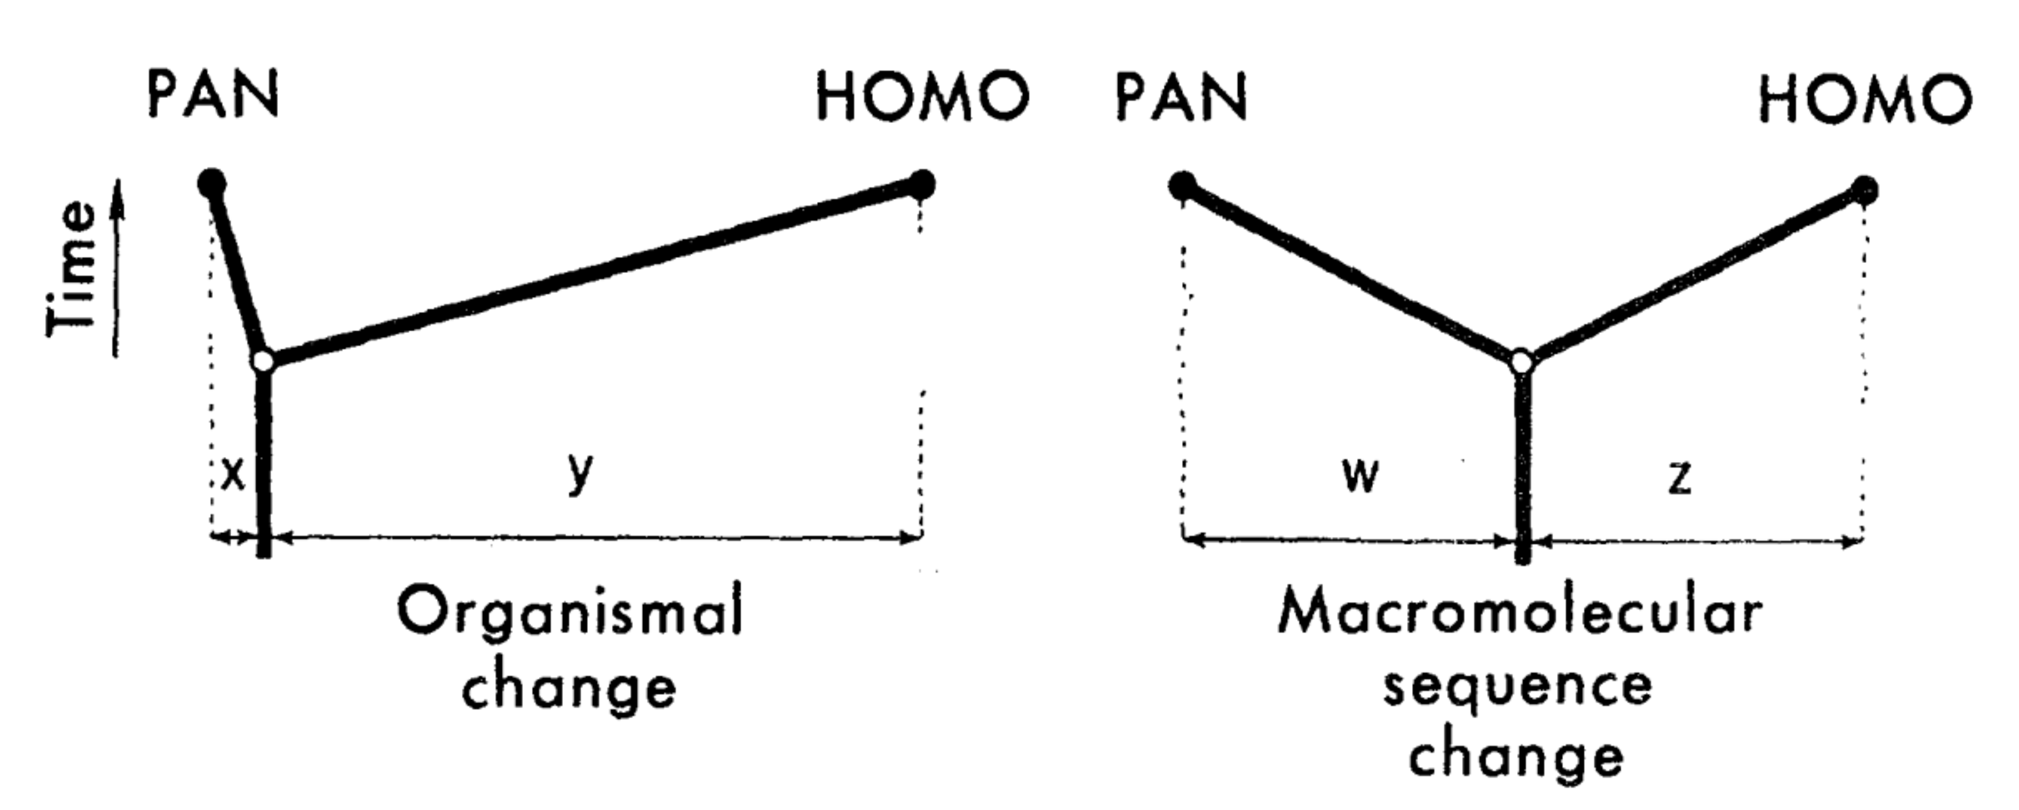
\includegraphics[scale=0.35]{Figs/king_wilson.pdf}
\caption{Schematic diagram of the rates of organismal and molecular
  change in human (Homo) and chimpanzee (Pan). Figure taken from
  \citet{King1975}.}
\label{fig_king_wilson}
\end{figure}

Continued genetic, anatomical and behavioral study of primates has
somewhat tempered the imbalance in the ``organismal'' rates of human
and chimpanzee evolution as drawn by King and Wilson: the evolution of
human form does not appear to be exceptional within the context of
other mammalian and primate species \citep{Carroll2003}, and humans
variously share and differ in many behavioral and sexual
characteristics with chimpanzee and gorilla
\citep{Harcourt1980,Goodall1986,Vigilant2004}. On the molecular level,
however, few plausible connections between human-specific phenotypes
and molecular changes have been found, lending support to King and
Wilson's 30-year old prediction
\citep{Clark2003,Sequencing2005a,Bradley2008}. In the first comparison
of the human and chimpanzee genomes, \citet{Sequencing2005a} wrote
that ``We thus find minimal evidence of acceleration unique to either
the human or chimpanzee lineage across broad functional categories.''
Still, these general findings do not preclude the possibility of
\emph{some} amount of protein-coding change playing a role in the
differences between humans and our close relatives. Studies of
protein-coding evolution in humans and other great apes have provided
insight into the evolution of primates as a whole, identifying
patterns of adaptive evolution or relaxed constraint in genes related
to sound perception \citep{Clark2003}, coloration \citep{Mundy2007},
language \citep{Enard2002} and brain size
\citep{Montgomery2011}. Adaptive evolution in genes related to sperm
production \citep{Clark2005} and immune defense \citep{Sawyer2005a}
has also repeatedly been found in primates, though these patterns of
selective pressures appear to be shared throughout the mammalian
clade, as evinced in Chapter \ref{ch_mammals2}.

Within this context, the recent sequencing of a western lowland
gorilla genome provided an opportunity to further examine patterns of
molecular evolution within human and our closest living relatives,
even if the power to detect lineage-specific adaptive events was
likely to be limited and the prevalence of such events is still
debated. Previous phylogenetic estimates indicated that the \ac{hcg}
common ancestor lived 6-10 \ac{myr} ago, with humans and chimpanzees
diverging a few \ac{myr} after that \citep{Bradley2008}. The inclusion
of gorilla into a sequence analysis would thus allow methods to make a
distinction between substitutions along the more distant \ac{hcg} and
the more recent \ac{hc} ancestral branches of the phylogeny. The
inclusion of gorilla within a comparative analysis would also provide
6-10 \ac{myr} of additional branch length to the primate tree,
possibly providing additional information regarding the constancy or
variability of evolutionary rates in the recent evolution of the
\acp{aga} (e.g., human, chimpanzee and gorilla). Previous analyses have
estimated a greater \ac{ne} in chimpanzee compared to human
\citep{Sequencing2005a,Siepel2009a}, and somewhat surprisingly, one
study identified more lineage-specific \acp{psg} in chimpanzee than in
human (\citet{Bakewell2007}, but see \citet{Mallick2009} for evidence
of false positives in these results). Gorilla, representing a third
independent \ac{aga} lineage with a slightly longer terminal branch
length than human and chimpanzee, could provide an important
additional data point in this regard.

In collaboration with Stephen Montgomery and Nick Mundy from the
Zoology department of Cambridge University, I performed an analysis of
the evolution of protein-coding genes in gorilla and the \ac{aga}. The
analysis was jointly designed by Stephen, Nick and myself; all data
collection, calculations and statistical analyses were performed by
me; and results were interpreted by us and other members of the
gorilla analysis consortium. As with the analysis for the \acl{mgp}, a
summary of our main findings was contributed to the manuscript
describing the gorilla genome, which is currently undergoing peer
review. The description of the methods and results presented here is
similar to the text included in the submitted manuscript and
supplementary documents.

The main focus of this analysis was to use codon models of evolution
to identify genes with accelerated \nsyn substitution rates in the
terminal and ancestral branches of the \ac{aga}. To do this, I
collected a highly filtered set of coding alignments in six primate
species (the \acp{aga} plus orangutan, rhesus macaque, and
marmoset) and used a series of \acp{lrt} based on the branch models
implemented in \acsu{paml} to identify accelerated genes along branches
of the primate phylogeny. Within the wider context of the gorilla
genome analysis, which included an investigation of \ac{ils} in coding
and non-coding regions, a secondary goal of this study was to identify
patterns of \ac{ils} within and near protein-coding genes. A third
goal was to use the set of genome-wide coding alignments to estimate
lineage-specific average \dnds ratios. Through the connection between
\ac{ne} and \dnds, these results could be used to place gorilla and
the ancestral \ac{aga} branches within the wider context of changing
primate population sizes through time \citep{Sequencing2005a}.

\section{Data collection and quality control}
\subsection{Primate one-to-one orthologous genes}

All orthologous gene sets, gene trees, and sequence alignments were
collected from Ensembl Compara release 60 using the Ensembl Perl API
\citep{Vilella2009,Flicek2011}. I first identified the set of genes
sharing one-to-one orthology among all six primates by collecting
homology annotations from the \ens \cmp database: for each human
protein-coding gene, the orthology status for each non-human species
was assigned to different categories based on the number of homologous
genes and the type of homology as annotated by \ens. Homologs were
classified as either one-to-one (e.g., one homolog available and
either an ``ortholog\_one2one'' or ``apparent\_ortholog\_one2one''
homology type), deleted (e.g., no homolog available), duplicated
(e.g., multiple homologs available), or human duplication (e.g., one
homolog available but containing an ``ortholog\_one2many'' annotation,
indicating that there are multiple human homologs for that single
non-human homolog). From an initial set of 20,746 human protein-coding
genes, this procedure identified 12,652 genes with 6-way 1-to-1
orthology; 4,809 genes with primate deletions; 1,171 genes with
primate duplications; 308 genes with human-specific duplications; and
1,806 genes with mixed patterns of duplication and deletion.

%Figure \ref{fig_gorilla_dup_dels} shows two Venn diagrams of shared
%gene deletions and duplications in chimpanzee, gorilla, orangutan and
%macaque relative to the human set of protein-coding genes. The \emph{a
%  priori} expectation, assuming somewhat random ongoing process of
%gene duplication and deletion, was that species most closely related
%to human would contain fewer deletions and duplications relative to
%the human gene set, with increasingly distant species having greater
%numbers. Ignoring the overlap, a comparison of the size of each
%species' circle in Figure \ref{fig_gorilla_dup_dels}A showed this to
%be the case: 2,279 deletions were found for chimpanzee, 2,344 for
%gorilla, 3,050 for orangutan, and 3,015 for macaque (marmoset, not
%shown, had 3,215 deletions). The counts of duplications showed a
%similar pattern, except for a notable excess of gorilla duplications:
%gorilla had 273 duplications relative to human, compared to 74 in
%chimpanzee, 165 in orangutan, 522 in macaque, and 722 in marmoset. The
%excess of duplications in gorilla appeared to be anomalous, and is
%expected to decrease in future refined versions of the gene annotation
%set.

%\begin{figure}
%\centering
%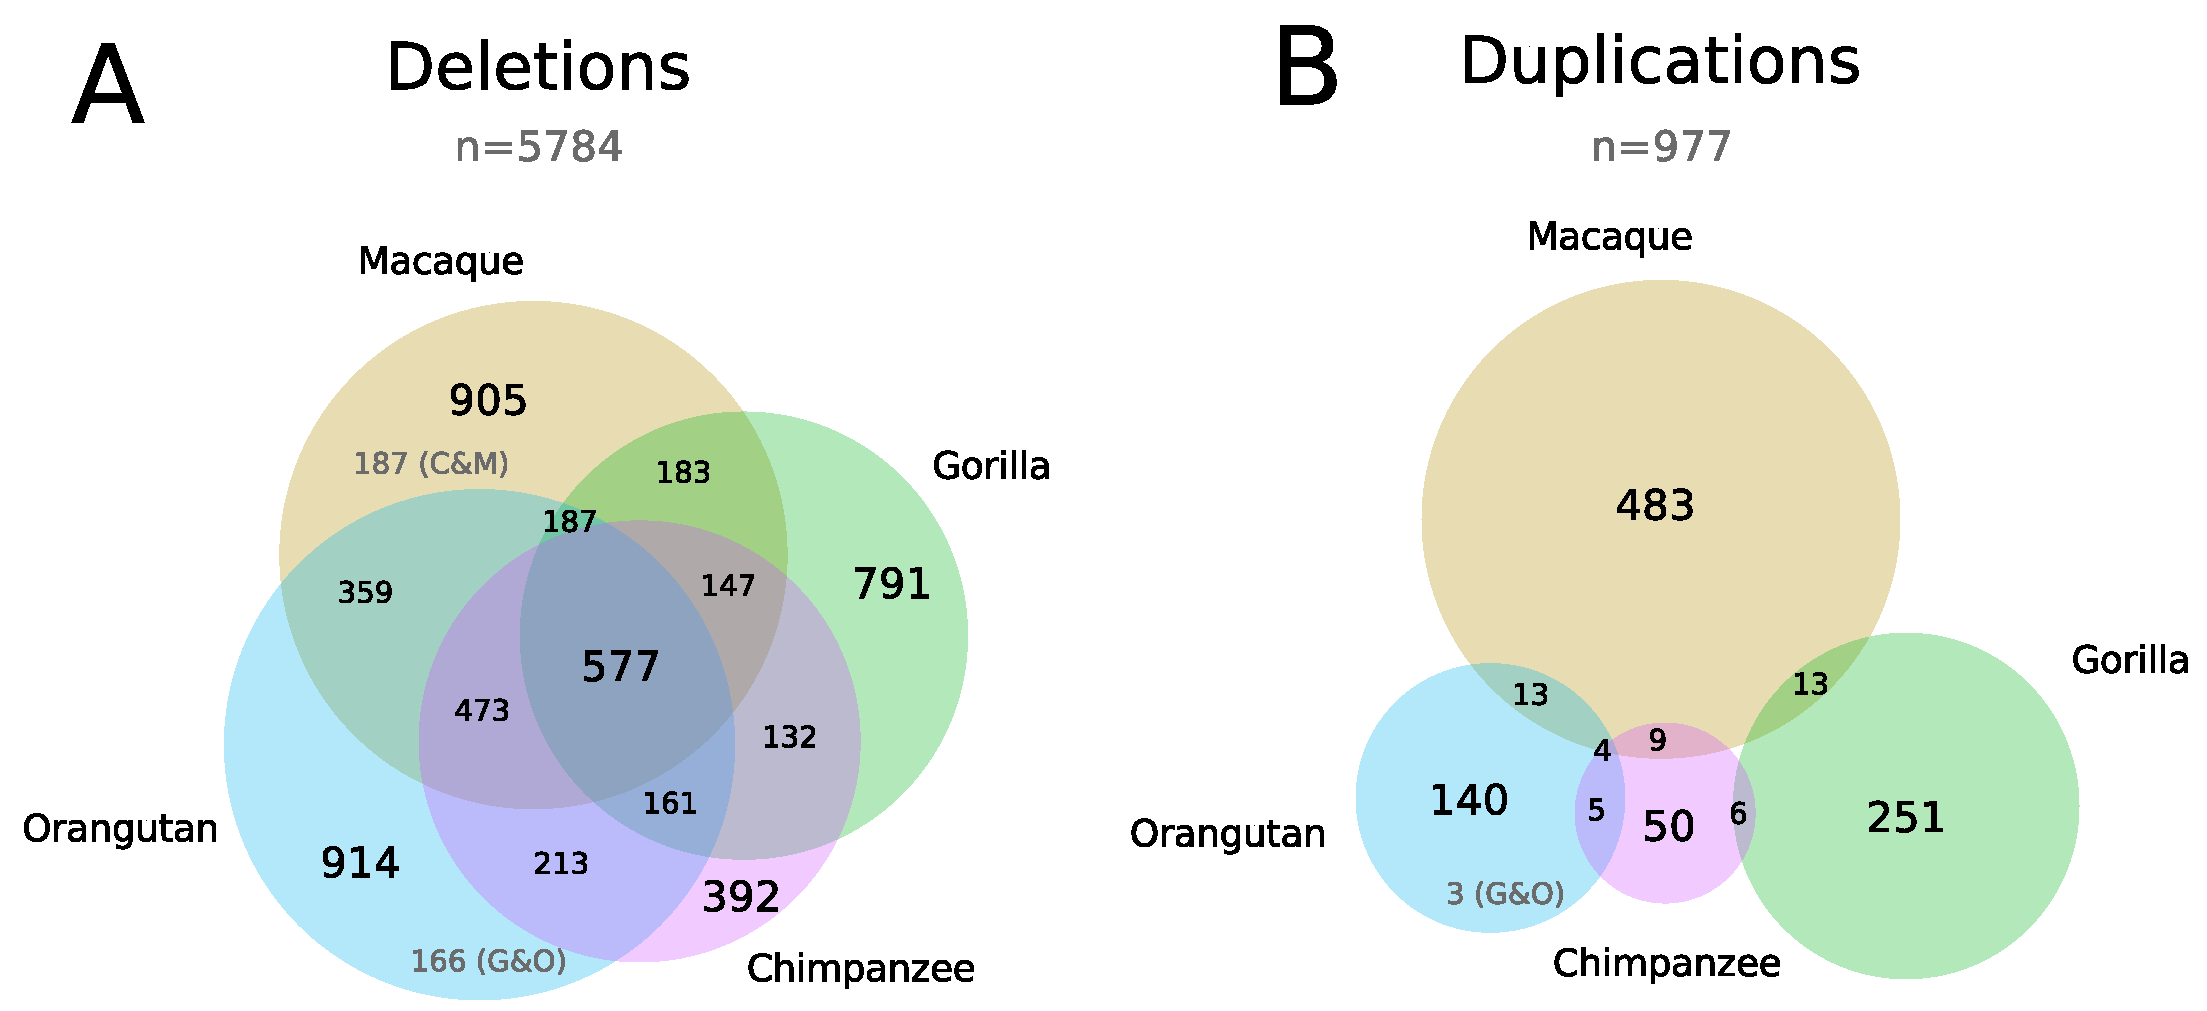
\includegraphics[scale=0.4]{Figs/gorilla_dup_dels.pdf}
%\caption{Venn diagrams of shared and unique (A) deletions and (B)
%  duplications in non-human primates relative to the set of human
%  genes.}
%\label{fig_gorilla_dup_dels}
%\end{figure}

%The amount of overlap between species in the Venn diagrams of Figure
%\ref{fig_gorilla_dup_dels} shows how often deletions and duplications
%relative to human are shared between different primate
%species. Interestingly, deletions appeared to be more often shared
%between two or more species than duplications, suggesting that certain
%genes may be more prone to independent deletion events than
%duplication events. It should be stressed, however, that this analysis
%and view of gene duplications and deletions was not intended to
%rigorously identify gene duplication and deletion events in
%primates. A more appropriate approach would be to explicitly place
%duplication and deletion events along the primate phylogeny using one
%or multiple mammalian outgroups, but these comparisons were made
%mostly to gain an understanding of whether gene deletions or
%duplications were more responsible for genes which did not have
%one-to-one orthology within \ac{aga}.

%\begin{figure}
%\centering
%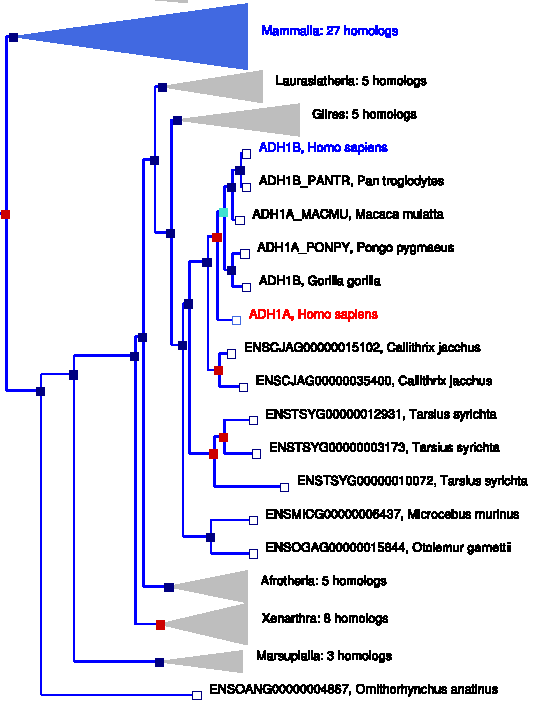
\includegraphics[scale=0.9]{Figs/adh1a.pdf}
%\caption{Part of the inferred gene tree relating the human gene
%  \gene{ADH1A} and its homologs. \gene{ADH1A} is highlighted in red
%  and the human gene \gene{ADH1B} is highlighted in blue. The gene
%  tree data were taken from \ens release 60.}
%\label{fig_adh1a}
%\end{figure}

%Many of the shared deletions in Figure \ref{fig_gorilla_dup_dels} were
%likely the result of recent human duplications where the homology to
%other primate genes was not detected, either due to incorrect
%assembly, missing primate gene annotations or the conservative rules
%used by \ens to assign orthology relationships based on gene trees
%\citep{Vilella2009}. An example is the gene \gene{ADH1A}: although the
%homology annotations indicated the gene as lacking a homolog in all 5
%of the primates included here, a detailed analysis of \gene{ADH} gene
%family evolution identified clear one-to-one orthology between
%\gene{ADH1A} genes within primates \citep{Oota2007}. The authors
%showed that the cluster of \gene{ADH} genes likely arose through
%mammalian-specific and primate-specific duplication events in
%chromosome 4, raising the possibility that these duplicated genomic
%segments could have been falsely collapsed into a single assembled
%sequence in non-human assemblies. The \cmp gene tree for \gene{ADH1A},
%pictured in Figure \ref{fig_adh1a}, shows that some primate species
%are missing annotated \gene{ADH1A} or \gene{ADH1B} orthologs,
%consistent with a collapsed assembly in that region. Perhaps as a
%result of these missing orthologs, the human \gene{ADH1A} is placed as
%an outgroup to the entire clade of \ac{aga} \gene{ADH1} orthologs,
%causing it to be annotated as lacking human orthology in the \ac{aga}
%species. In addition to illustrating the problems involved in
%identifying orthology between highly-duplicated genes in
%closely-related species, this example showed that the \ens one-to-one
%orthology annotations were conservative. The 12,652 one-to-one
%orthologs identified using these annotations were selected for further
%analysis.

\subsection{Collecting and filtering six-way codon alignments for one-to-one genes}
\label{sec_ils_mask}

Codon alignments of all one-to-one orthologs were extracted from the
6-way primate genomic alignments pre-calculated by the \ens pipeline
using the \ac{epo} pipeline \citep{Paten2008a,Paten2008}. I extracted
and concatenated primate alignment blocks corresponding to the
protein-coding portion of each exon from the consensus coding
transcript of each human gene. These alignments were then flattened to
the human reference by removing all columns with insertions in
non-human primates or deletions in the human lineage. Since the
\ac{epo} alignments are generated on the DNA level and the current
evolutionary analysis was to be performed on the codon level, I
clearned each alignment for codon analysis by masking out any triplets
containing stop codons or out-of-frame gaps. Of the original 12,562
one-to-one genes identified above, 11,538 codon alignments were
successfully collected. The reduction numbers came from 1,024 genes
which were discarded because an entire species was missing from that
region of the primate \ac{epo} alignment; the species most often
missing in the alignments were orangutan (520 genes), marmoset (475 genes),
and macaque (328 genes).

The low levels of divergence between the primate species being
analyzed made it extremely important to avoid the inclusion of any
incorrectly-aligned material. The expected number of lineage-specific
substitutions per gene scales linearly with the length of that
species' terminal branch, meaning a small number of sequencing,
assembly or alignment errors causing apparent \nsyn substitutions
along one of the short \ac{aga} terminal lineages could easily lead to
a false positive inference of accelerated evolution. As such, an
aggressive set of filters was applied to each alignment prior to the
\ac{paml} analysis.

First, the chimpanzee, orangutan, macaque and marmoset sequences were
filtered using Phred or Phred-like quality scores downloaded from the
UCSC (chimpanzee and macaque) or WUSTL (orangutan and marmoset)
websites. Any bases with a quality score lower than 30 (corresponding
to an expected error rate of 1 in 1000 bases) were replaced with `N's.

An initial analysis of the Phred filtered 6-way alignments revealed
many stretches of alignment with obviously non-homologous sequence in
one or more non-human genomes. These regions appeared similar to the
clustered substitutions seen in Chapter \ref{ch_mammals1}, although
alternative splicing or mis-annotated genes could be ruled out as a
causative factor since the EPO alignments were built on the DNA level
and only the human transcript structure was used. The most likely
cause was some combination of mis-assembled genomic sequence and
misalignment by the EPO pipeline. I found that genes containing these
dubious aligned stretches were prominent among the initial list of
accelerated genes based on these alignments.

To exclude such regions from analysis, I applied a filter based on
windows of inferred lineage-specific substitutions, using an approach
similar to that described for the filtering of mammalian alignments in
Chapter \ref{ch_mammals1}. First, the codon alignment was analysed
with the codeml program of \ac{paml} v4.14 using a M0 model to infer
substitutions in the terminal lineages of the 6-species tree. Using
the branch lengths (expressed as the expected number of substitutions
per codon) and substitution evens inferred by \ac{paml}, I analyzed
the density of codons containing lineage-specific non-synonymous
substitutions within every 15-codon window along the alignment. Any
window containing more than 10 \nsyn substitutions per codon per unit
of branch length was masked with `N's. After analyzing the preliminary
results from this method, a number of additional heuristic corrections
were made to avoid excess stringency or lenience: first, branch
lengths below 0.05 substitutions per codon were set to 0.05 in order
to avoid too small of a denominator; second, the masking threshold was
decreased from 10 to 5 for any windows overlapping alignment gaps or
ambiguous nucleotides; third, codons containing two or three
nucleotide substitutions along one branch were counted as two \nsyn
substitutions.

This procedure resulted in a total of 72,729 nucleotides being masked
from 1,156 genes, with the following breakdown of the numbers of genes
in which each species had at least one nucleotide masked: 12 human,
195 chimpanzee, 232 gorilla, 296 orangutan, 271 macaque and 324
marmoset.  The low number of genes from which any human sequence was
masked indicated that the filtering was not overly conservative, while
the high numbers in non-human primates indicated that those genomes
are more likely to contain highly localized, apparently spurious runs
of \nsyn substitutions in the regions of EPO alignments corresponding
human transcripts.

A final filter was applied to avoid a potential bias from
substitutions in regions of \ac{ils} between sequences in human,
chimpanzee, and gorilla. \ac{ils} regions are genomic segments where
either gorilla-chimpanzee or gorilla-human share a most recent common
ancestor, deviating from the ``canonical'' relationship where human
and chimpanzee share the most recent ancestor. Roughly 20-30\% of the
genome shows evidence of \ac{ils} within the African great apes
\citep{Hobolth2007}. In cases where a \syn or \nsyn substitution
occurs along the ancestral branch of a genomic segment subject to ILS,
the assumption of a single phylogenetic tree per gene is violated and
\ac{paml} cannot correctly infer a single substitution event. Instead,
two substitutions must be inferred in order to fit the observed site
pattern to the canonical phylogenetic tree. The method can choose to
infer either two identical substitutions (one along each of the
terminal ``ILS'' branches sharing the most recent common ancestor) or
one substitution along the \ac{hcg} ancestral branch and a second
reversion substitution along the non-ILS terminal branch. I observed
that PAML tended to infer the latter sequence of events as the most
likely substitution history. The long length of the \ac{hcg} ancestral
branch may have contributed to the two-substitution path being the
most likely one.

Given the high proportion of expected sites under \ac{ils}, I applied
a simple filtering method to mask out codons that were likely the
result of a single substitution in an ancestral \ac{ils} lineage. Any
codon where either gorilla-human or gorilla-chimpanzee shared a codon
sequence that was different from both orangutan and the non-\ac{ils}
species (either human or chimpanzee) was considered likely to contain
an ancestral \ac{ils} substitution. The human, chimpanzee and gorilla
sequences at these sites were all masked with `N's, causing \ac{paml}
to treat those nucleotides as missing data. This resulted in 7,841
codons being masked from 4,340 genes prior to analysis with
\ac{paml}. Although the \ac{ils} masking was relatively widespread
across genes, its effect on the results was conservative with respect
to the number of inferred substitutions, and likely had a minimal
impact on the identification of accelerated genes: the majority of
genes (2,605) contained only one masked codon, which would be unlikely
to seriously attenuate an otherwise strong signal of lineage-specific
acceleration.

\subsection{Manual identification of remaining alignment or assembly errors}

A manual analysis of genes with suspiciously strong evidence for an
accelerated \nsyn substitution rate identified 4 genes with apparent
alignment or assembly error that escaped the various filtering steps
described above. (Note that the \ac{lrt} method designed to test for
lineage-specific acceleration is described in Section
\ref{sec_accel_lrt}.) For each potentially erroneous gene, a manual
analysis of the alignment was undertaken by visually inspecting the
codon alignment, the locations of inferred substitutions, and the
protein-based alignment of the same gene downloaded from v60 of the
\ens \cmp database. In total, 4 genes---\gene{ITPK1}, \gene{POLR2A},
\gene{ATN1}, and \gene{GAS6}---were found to show evidence of serious
misalignment and were removed from further analysis. Two other genes,
\gene{SUPT16H} and \gene{POLR1A}, contained similarly strong signals
of lineage-specific acceleration and elevated numbers of \nsyn and
\syn substitutions. These genes were also manually assessed, but no
obvious signs of misalignment were found. The four genes with clear
errors were removed from the set of genes analyzed for the remainder
of the analysis, resulting in 11,534 total genes analyzed by the
\acp{lrt} described below.


%\gene{ITPK1}, which codes for an inositol triphosphate kinase with 415
%amino acids and had a primate \dnds of 0.094 (as estimated from
%\ac{paml} using the M0 model), showed 28 \nsyn and 10 \syn
%substitutions in the chimpanzee lineage and a strong signal for
%chimpanzee acceleration. The alignment showed few chimpanzee
%substitutions in the first half of the protein, but a high density of
%masked chimpanzee nucleotides and mixed synonymous and \nsyn
%chimpanzee substitutions in the second half. The substitutions that
%were not masked by the window-based filter were presumably just below
%the threshold used. I analyzed the alternative protein-based
%alignments from \ens \cmp, which included a different stretch of
%sequence for the chimpanzee \gene{ITPK1} ortholog in the second half
%of the protein. This sequence had far fewer mismatches, indicating
%that the \ac{epo} genomic alignments from which our data were
%generated contained a chimpanzee misalignment in the latter half of
%the protein.

%\gene{POLR2A}, which codes for the largest subunit of RNA polymerase
%II with 1,971 amino acids and a primate \dnds of 0.043, contained 22
%\nsyn and 70 \syn substitutions in the gorilla lineage and a strong
%signal for gorilla \dn acceleration. The gene showed a highly
%conserved pattern across the bulk of its length, except for the final
%250-300 amino acids which contained a highly repetitive sequence and
%long, dense clusters of substitutions in both gorilla and
%orangutan. The protein-based alignments showed a much cleaner gorilla
%sequence, but stretches of spurious substitutions were instead found
%in the chimpanzee sequence, suggesting that this repetitive region is
%subject to frequent genome assembly and/or alignment error.

%\gene{ATN1} codes for a protein of unknown function which, upon the
%expansion of a trinucleotide repeat within the region, leads to
%dentatorubral pallidoluysian atrophy, a rare neurodegenerative
%disorder \citep{OkamuraOho1999}. With 1,191 amino acids and a
%relatively high primate \dnds of 0.339, \gene{ATN1} showed 105 \nsyn
%and 54 \syn substitutions in gorilla, with a strong signal for
%acceleration. The gorilla substitutions were evenly interspersed along
%the length of the gene, but they were noticeably absent from the first
%and last 100 amino acids. Gorilla also showed a long 50-amino acid gap
%prior to the high-substitution region. A comparison to the
%protein-based alignments did not show a different gorilla sequence;
%rather, it contained a chimpanzee sequence with a similar pattern of
%high numbers of substitutions. This suggested that there may be a
%duplicated or pseudogenic version of the gene region in primates which
%contains many substitutions relative to the \gene{ATN1} gene. Thus, it
%was likely that the pattern of gorilla substitutions seen in the
%\gene{ATN1} alignment was not indicative of substitutions acting on a
%functional ortholog of human \gene{ATN1}. 

%\gene{GAS6} codes for a protein thought to be involved in the
%stimulation of cell proliferation. It contains 722 amino acids, has a
%primate \dnds of 0.150, and contained 29 \nsyn and 8 \nsyn gorilla
%substitutions and yielded a strong signal for gorilla
%acceleration. Manual analysis of the alignment revealed a block of
%\nsyn substitutions in the middle of the gene directly adjacent to a
%block of sites which were masked by the window-based filter. The
%protein-based alignments contained a different gorilla sequence in the
%concerned region, but this different sequence contained a
%qualitatively similar number of differences relative to human.

\section{Codon model evolutionary analysis}

The set of evolutionary models and \acp{lrt} used to identify
accelerated genes in the 6-way primate alignments were designed by
Stephen Montgomery, Nick Mundy and myself.

\begin{figure}
\centering
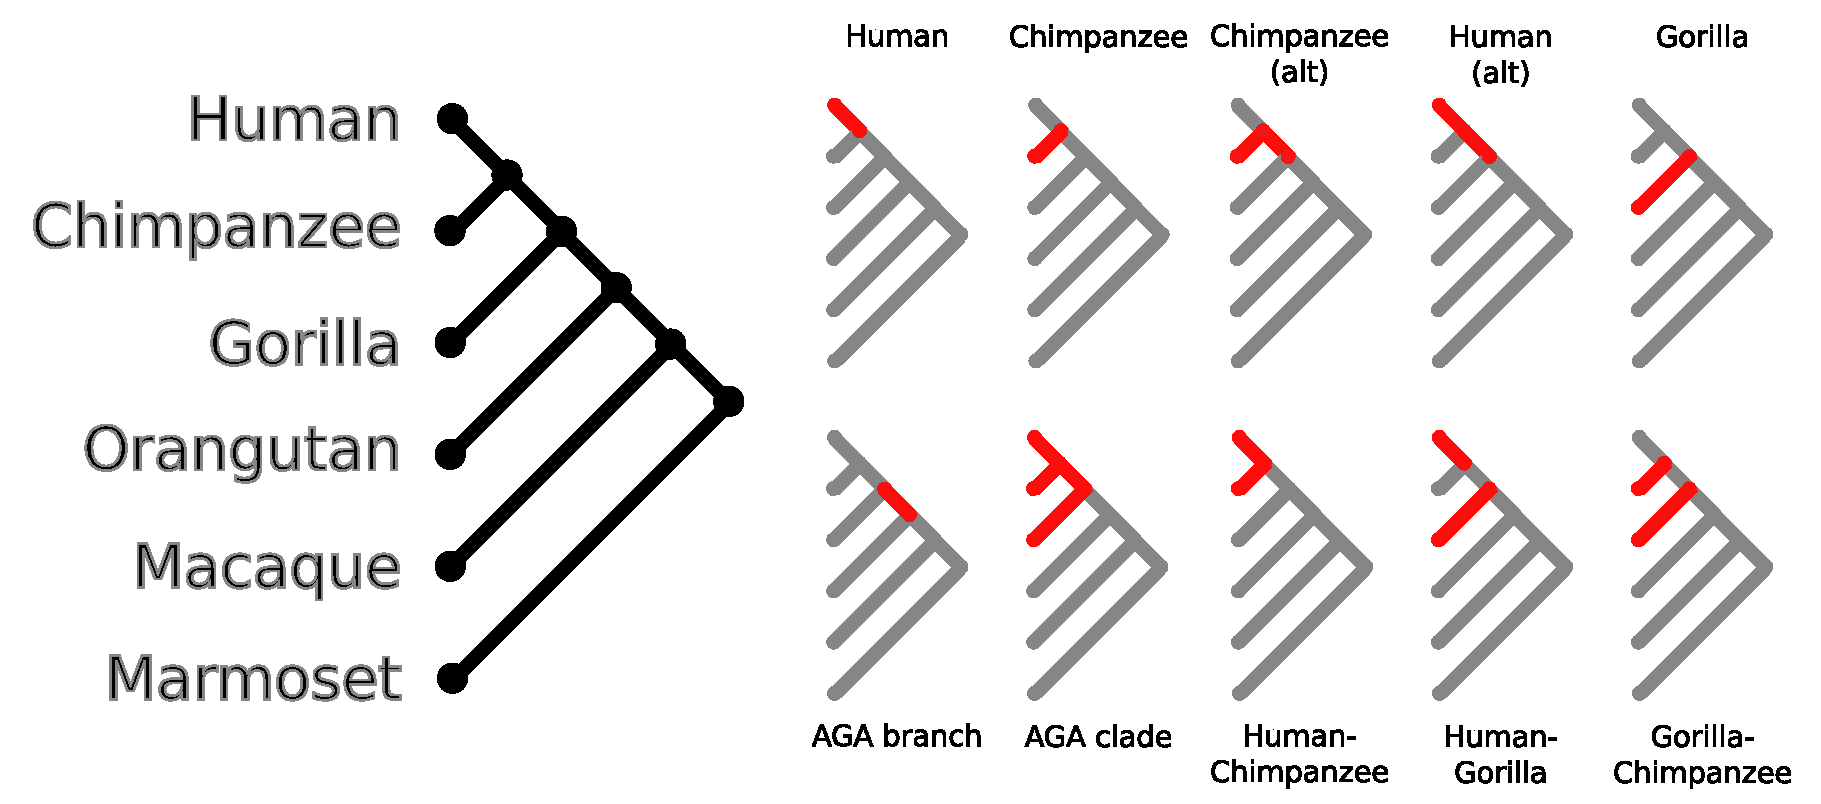
\includegraphics[scale=0.5]{Figs/gorilla_branch_models.pdf}
\caption{Branch models used to construct \ac{lrt} for detecting
  accelerated genes in various branches of the \ac{aga} phylogeny. The
  foreground branches for each model are highlighted in red. The label
  above or below each tree describes which species or group of species
  is under investigation with each model. AGA---African great apes;
  alt.---alternative model.}
\label{fig_gorilla_branch_models}
\end{figure}

To detect signals of accelerated and decelerated evolution in gorilla
and the \ac{aga}, a total of 10 so-called branch models of evolution
were specified. Each branch model separates the phylogenetic tree into
two categories of branches, foreground and background branches, which
are then modeled as evolving with separate \dnds ratios by including
distinct foreground and background \omg parameters in the model
\citep{Yang1998,Yang1998a}. Figure \ref{fig_gorilla_branch_models}
shows the models used in this study, with background branches in gray
and foreground branches in red. Each branch model was designed to
allow for an elevated (accelerated) or decreased (decelerated) \dnds
ratio in a branches of particular interest to the study of \ac{aga}
evolution. \ac{paml} was used to estimate parameters and calculate the
likelihood value for each model in Figure
\ref{fig_gorilla_branch_models} applied to each coding alignment. A
\ac{lrt} was performed for each model by comparing the likelihood of
the alignment under that branch model to the likelihood of the
alignment under the simpler M0 model, which uses a single \omg
parameter for the entire tree. This test will be referred to as a
branch-LRT to distinguish it from the more commonly used branch-site
LRT described below. The branch-LRT statistic represents the strength
of evidence that a given branch model is a better fit than the simpler
M0 model to a given alignment; in other words, a large statistic can
be interpreted as an indication that the evolution of the gene is
well-explained by different \dnds ratios in the foreground and
background branches of the tree. The \ac{ml} estimate of the two \omg
parameters could be used to identify genes where the estimated
foreground \omg was higher or lower than the background. Genes where
the foreground \omg was higher than the background were categorized as
accelerations, and genes where the foreground \omg was lower than the
background were categorized as decelerations. Using the \ac{lrt}
statistic and the distinction between accelerations and decelerations,
a signed \ac{lrt} statistic was constructed for each branch-LRT, where
accelerated genes were assigned the branch-LRT statistic and
decelerated genes were assigned the negative of the branch-LRT
statistic. In this way, a single number was used to encapsulate the
direction and strength of evidence in support of a shifted \dnds ratio
in the foreground branch of each model presented in Figure
\ref{fig_gorilla_branch_models}.

A highly positive signed branch-LRT score represented strong evidence
for a lineage-specific elevated \dnds ratio. Such an elevated ratio
could be explained either by positive selection or relaxed constraint
\citep{Nielsen2005,Sequencing2005a}. To attempt to distinguish the
former from the latter, I used the branch-site \ac{lrt} implemented in
\ac{paml} \citep{Zhang2005} to identify genes with significant
evidence for positive selection acting along a branch or
clade. Similar to the branch-LRT, the branch-site LRT requires a
predefined separation of branches into foreground and background
categories. However, the branch-site LRT is specifically tuned towards
identifying temporally and spatially localized episodes of positive
selection \citep{Nielsen1998,Yang2002b,Zhang2005}. The branch-site LRT
was run for the Human, Chimpanzee, Gorilla, AGA branch and AGA blade
models shown in Figure \ref{fig_gorilla_branch_models}.

For each model tested, the full length codon alignment was input to
the \texttt{codeml} program from the \ac{paml} package along with a
phylogenetic tree corresponding to the accepted species tree structure
(the labeled tree in Figure \ref{fig_gorilla_branch_models}). The
`cleandata’ option was set to 0 (e.g., alignment columns containing
gaps were not removed from the analysis but were treated as ambiguous
data), and branch lengths inferred by \texttt{codeml} based on the
initial M0 model model analysis were used as the initial branch
lengths for all other models tested.

When the null model of evolution in the branch-LRT is true, the
ac{lrt} statistic---measured as twice the difference in log-likelihood
values between the branch model and the null M0 model---should be
distributed according to a \chisq distribution with one degree of
freedom. The same null distribution was assumed for the branch-site
LRT. Strictly speaking, the branch-site LRT null distribution should
be a 50:50 mixture of a point mass at 0 and \chisq with one degree of
freedom, but the more conservative \chisq distribution is recommended
by Ziheng Yang to guard against violations of model assumptions
\citep{Yang2007}. \pvs for each branch-LRT and branch-site LRT result
were thus calculated by comparing the absolute value of the \ac{lrt}
statistic to a chi-squared distribution with 1 degree of freedom. The
Benjamini-Hochberg method \citep{Benjamini1995} was used to correct
for multiple testing within each branch model by controlling the
\ac{fdr}.

The ``alternative'' models shown in Figure
\ref{fig_gorilla_branch_models}, which were designed to detect
accelerations along the human and chimpanzee lineages while correcting
for the difference in branch length between the human-chimpanzee
terminal branches and the gorilla terminal branch, did not yield
qualitatively different results from the equivalent uncorrected
models. To simplify the discussion, results from those tests were
discarded from the rest of the analysis.

\subsection{Branch-LRT and branch-site LRT results}

\begin{table}
\centering \scriptsize
\begin{tabular}{lrrrrrr}
\toprule
 & \multicolumn{2}{c}{Acceleration} & \multicolumn{2}{c}{Deceleration} & \multicolumn{2}{c}{Branch-site LRT} \\
Model / Species & $p<0.05$ & FDR$<0.1$ & $p<0.05$ & FDR$<0.1$ & $p<0.05$ & FDR$<0.1$ \\
  \midrule

\input{Tables/gorilla_lrt_results.txt}
\bottomrule
\end{tabular}
\caption{A summary of the branch-LRT and branch-site LRT results. Each
  row corresponds to a model in Figure
  \ref{fig_gorilla_branch_models}, except for the two ``alternative''
  models, which were excluded from the analysis. Each cell represents
  the number of genes for which the \ac{lrt} was significant at the
  specified threshold for the given model. \pvs were calculated by
  comparing the \ac{lrt} statistic to a \chisq distribution with one
  degree of freedom. The \acf{fdr} was controlled within each model
  separately for the branch-LRTs and for the branch-site LRTs using
  the \citet{Benjamini1995} method.}
\label{table_gorilla_lrt_results}
\end{table}

Table \ref{table_gorilla_lrt_results} presents for each model, and at
two significance thresholds ($p<0.05$ and LRT$<0.1$), the number of
significantly accelerated and decelerated genes according to the
branch-LRT and the number of positively-selected genes according to
the branch-site LRT. The number of $p<0.05$ accelerated genes for
almost all of the branch models was greater than the expected number
under the null model. Assuming equivalent amounts of acceleration and
deceleration, the expected number of $p<0.05$ accelerations and
decelerations using the branch LRT would be roughly
$11,538\times0.05/2=288$ genes. All models showed an excess of
accelerated genes, with between 300 and 873 genes accelerated at the
nominal $p<0.05$ threshold. Significant evidence for deceleration, was
found at levels equal to or slightly below the null expectation, with
between 151 and 314 decelerations per model. The ``AGA Branch'' model
showed a notable tendency towards lower \dnds ratios, with the fewest
accelerations (300) and most decelerations (314) out of all models
tested.

Looking at strongly accelerated or decelerated genes, defined as those
corresponding to $FDR<0.1$, roughly equivalent numbers were found in
the three terminal lineage models (human / chimpanzee / gorilla) with
between 10-19 strong accelerations and between 1-2 strong
decelerations for each model. The other models were much more
variable, possibly due to differences in power resulting from
different foreground branch lengths, with the AGA Clade model showing
many strongly-shifted genes (56 strong accelerations and 9 strong
decelerations) and the AGA Stem model showing very few (3 strong
accelerations and 1 strong deceleration). The Human-Chimpanzee,
Gorilla-Human, and Gorilla-Chimpanzee models, designed to detect
evidence for parallel accelerations and decelerations, showed roughly
twice as many strongly accelerated and decelerated genes as their
terminal-branch counterparts (29-45 strong accelerations and 3-6
strong decelerations), as might be expected based on the doubled
amount of branch length in the foreground portions of their models.

\section{Parallel accelerations}
\label{sec_parallel_accel}

I used the lineage-specific gene acceleration LRT results to evaluate
the prevalence and strength of parallel gene accelerations between
\ac{gh}, \ac{gc}, and \ac{ch} during the time period since the
speciation of each pair. Parallel accelerations where analyzed on
three levels: first, quantifying genome-wide signals for shared gene
acceleration; second, identifying \ac{go} terms enriched for shared
accelerations; and third, identifying genes with the strongest
evidence of parallel accelerations for each species pair.

A suitable statistic by which to measure the amount of evidence for
parallel accelerations was first developed. Three of the branch models
shown in Figure \ref{fig_gorilla_branch_models} were designed to be
sensitive to parallel accelerations in the species pairs of interest
(e.g. the models labeled ``Human-Chimpanzee'', ``Human-Gorilla'', and
``Gorilla-Chimpanzee''), but I found that many of the strongest
branch-LRT results for these three models were driven by \nsyn
substitutions in primarily one of the two species pairs. For example,
\gene{SUPT16H}, the gene with the highest branch-LRT under the
``Human-Gorilla'', yielded a LRT score of 51.14. However, it appears
that most of this signal was due to substitutions in the gorilla
lineage: looking at the lineage-specific human and gorilla \ac{lrt}
values for the same gene, I found a gorilla LRT of 61.1 and a human
LRT of -1.34 (where a negative value indicated an estimated decrease
in \dnds relative to the background branches). Thus, human and gorilla
clearl did not both experience independently accelerated \dnds levels
in \gene{SUPT16H}, despite the strong LRT result from the
gorilla-human branch model. For this reason, LRT results from these
three ``parallel'' branch models were excluded from further
analysis. To ensure that genes identified as undergoing parallel
acceleration showed independent evidence in each lineage of having
experienced \dnds accelerations, I instead used the minimum of both
lineages' independent branch model LRT value as the statistic for
parallel acceleration in each pair of species. This statistic will be
referred to as \lrtmin. The counts of parallel accelerations and
decelerations shown in Table \ref{table_gorilla_lrt_results} were
calculated using the \lrtmin statistic for accelerations and an
equivalent LRT$_{max}$ statistic for decelerations (as the signed
\ac{lrt} statistic was negative for decelerated genes).

\subsection{Genome-wide rates of shared acceleration}

A randomized resampling strategy was used to determine whether the
number of parallel accelerations at a given branch-LRT cutoff
threshold was significantly greater than that expected given
independent distribution of each species' accelerated genes. For each
iteration of the randomization, a set of pseudo-``accelerated'' genes
for each paired species was chosen by randomly sampling $N_{acc}$
genes (where $N_{acc}$ is the number of observed lineage-specific
accelerations for each species at the given LRT cutoff threshold) from
among the 11,534 total genes. The number of overlapping accelerated
genes was counted at each iteration, and the fraction of iterations
which yielded a greater number of overlapping accelerations than the
observed number of parallel accelerations was taken as the \pv for the
significance of the observed number of overlapping accelerations at
the given cutoff threshold. This was repeated for each species pair,
and for cutoff thresholds ranging from 0 to 5.

The magnitude of over- or under-representation of parallel
accelerations was also estimated by calculating the co-occurrence
excess (defined as $N_{obs}/N_{exp} - 1$) of accelerated genes for
each pair of species and the same range of branch-LRT cutoff
thresholds. The expected number of parallel accelerations was
calculated using the same null expectation as the randomization test:
that each lineage has a proportion of accelerated genes, and that the
accelerations for each lineage are independently distributed amongst
the 11,534 total genes. The expected fraction of overlapping
accelerated genes is thus the product of each lineage's proportion of
accelerated genes, and $N_{exp}=N_{accA}/N\times N_{accB}/N\times N$
where $N$ is the total number of genes and $N_{accA}$ and $N_{accB}$
are the numbers of accelerated genes in each lineage. For each species
pair and cutoff threshold, one hundred bootstrap replicate datasets
were sampled from the 11,534 genes. The co-occurrence excess was
calculated for each replicate, and confidence intervals were
calculated at the 50\% level from the set of bootstrap values.

\begin{figure}
\centering
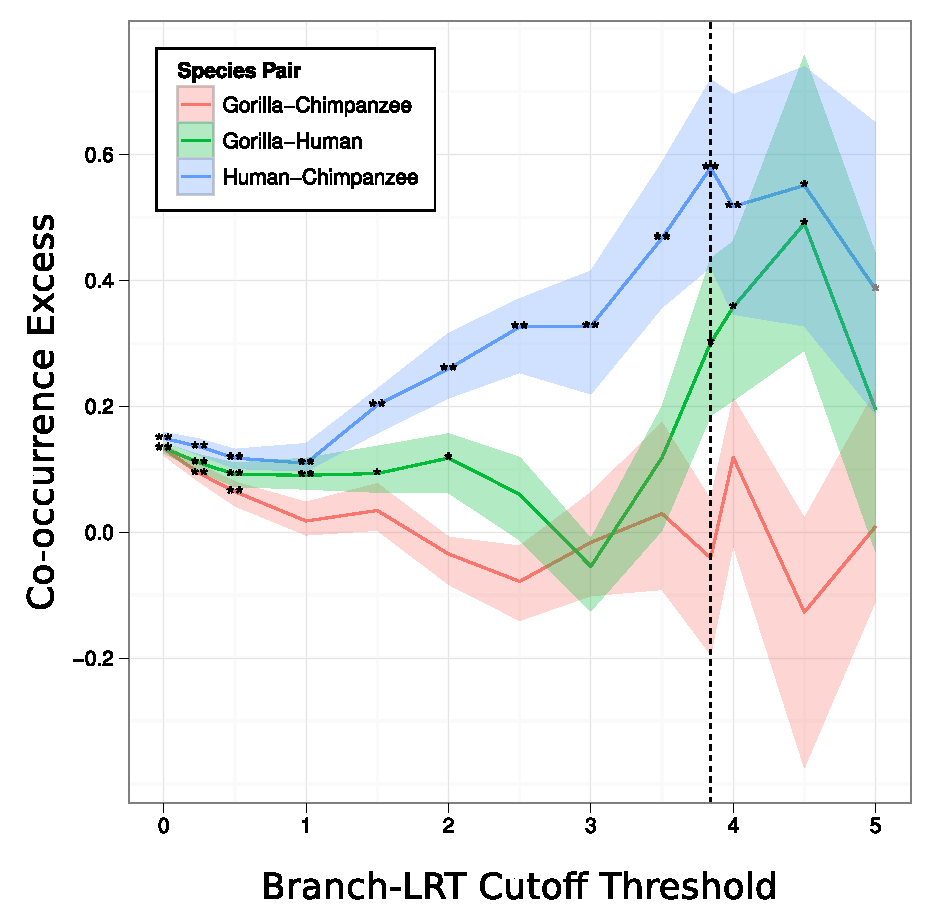
\includegraphics[scale=0.7]{Figs/gorilla_parallel.pdf}
\caption{Genome-wide excess of parallel accelerations in pairs of
  \ac{aga} species at various LRT cutoff values. Parallel gene
  accelerations in three species pairs (Gorilla-Chimpanzee, red;
  Gorilla-Human, green; Human-Chimpanzee, blue) were identified using
  branch model LRT cutoffs from 0 to 5 (x-axis; see text for details
  on how parallel accelerations were identified), and the
  co-occurrence excess between lineage-specific and parallel
  accelerations at each LRT cutoff was calculated (y-axis; the 50\%
  bootstrap confidence interval is shaded). A randomization procedure
  was used to identify significant enrichment for parallel
  accelerations: two black stars indicate $p<0.01$, one black star
  indicates $p<0.05$, and one gray star indicates $p<0.1$ for the
  given species pair and LRT cutoff. A vertical dotted line indicates
  the LRT cutoff corresponding to the 95\% chi-squared significance
  value.}
\label{fig_gorilla_parallel}
\end{figure}

The results of the randomisation test and co-occurrence calculations
are shown in Figure \ref{fig_gorilla_parallel}. For each species pair,
the co-occurrence excess is plotted as a function of the LRT cutoff
threshold with a solid line drawn at the co-occurrence value and a
shaded area drawn around the 50\% bootstrap confidence interval. The
results of the randomization test are indicated by one or two stars
drawn adjacent to the co-occurrence value for the given dataset. For
reference, a dotted vertical line is drawn at the LRT cutoff
corresponding to a nominal $p<0.05$ \chisq cutoff value. At lower
(i.e. more lenient) LRT cutoff values a greater number of genes in
each of the paired species were accelerated, and at higher (i.e. more
stringent) LRT cutoff values fewer genes are accelerated. This sample
size effect can be seen in the wider confidence intervals and larger
amounts of apparent stochastic noise at higher LRT cutoffs.

A trend was clear when comparing the co-occurrence excess levels and
randomisation test \pvs between the \ac{gh}, \ac{gc} and \ac{hc}
species pairs: \ac{hc} showed the largest excess of parallel
accelerations, \ac{gh} showed an intermediate amount of excess, and
\ac{gc} showed the least excess. This trend was consistent across a
wide range of threshold cutoff values and was supported by both the
co-occurrence excess values and the results of the randomisation
tests. The \ac{hc} species pair showed randomisation $p<0.01$ for all
but the two highest (i.e., most stringent) threshold cutoffs and a
maximum co-occurrence excess of nearly 60\%. The \ac{gh} species pair
showed significantly enriched acceleration overlap at $p<0.05$ for
threshold cutoffs below 2 and at 3.84, 4 and 4.5. The \ac{gh}
co-occurrence excess was noticeably lower than that of \ac{ch}, but
above zero for all but one threshold cutoff. The \ac{gc} species pair
showed little evidence of genome-wide enrichment for parallel
accelerations, with a significant overlap only at weak threshold
cutoffs of 0.5 or below and a co-occurrence excess hovering around
zero across the range of cutoff thresholds.

That the \ac{hc} pair showed the largest number of overlapping
accelerations was not entirely surprising, as human and chimpanzee
share the most recent speciation event among the three species
pairs. Thus, they presumably share the greatest number of
environmental and behavioral traits that might have caused a gene to
experience increased \nsyn substitutions in both lineages. More
interesting was the difference in overlap levels between the \ac{gc}
and \ac{gh} species pairs. Whereas the \ac{gc} pair showed little
genome-wide evidence for excess parallel acceleration, the \ac{gh}
pair showed a slight but consistent signal for more parallel
accelerations than expected by chance. This could be due either to a
greater degree of biological or environmental similarity in \ac{gh}
compared to \ac{gc}, or it could be the result of some underlying bias
in the data, such as differences between human and chimpanzee in
population size or genome quality.

\subsection{\ac{go} terms enriched in shared accelerated genes}

The second approach used to characterize genes with parallel
accelerations was to identify \ac{go} terms enriched for genes with
evidence for parallel acceleration in each pair of \ac{aga}
species. The methodology used to identify enriched \ac{go} terms will
be described Section \ref{sec_gorilla_go}, but the parallel results
are described here for continuity with the discussion of parallel
accelerations.

For each species pair, genes with \lrtmin$>1.5$ were considered
significant in the \ac{go} enrichment tests. This more lenient
threshold was used, since few genes were independently accelerated at
the 95\% chi-squared threshold of 3.84 in both lineages (25 genes for
\ac{gc}, 40 for \ac{gh}, and 51 for \ac{hc}; Table
\ref{table_gorilla_lrt_results}). At a \lrtmin threshold of 1.5, the
\ac{gc} pair yielded 206 accelerated genes, \ac{gh} yielded 238, and
\ac{hc} yielded 286. The sections of Table \ref{table_gorilla_go}
labeled ``Human-Chimpanzee Parallel'', ``Gorilla-Chimpanzee Parallel''
and ``Gorilla-Human Parallel'' show the terms most enriched for
parallel accelerations.

Although no species pair yielded \ac{go} terms significantly enriched
after correction for multiple testing, a number of terms were enriched
at a nominal $p<0.05$ significance using \ac{fet}. The top three terms
for \ac{hc} parallel accelerations were ``neuropeptide signaling
pathway'', ``regulation of DNA-dependent transcription'' and
``microtubule-based movement''; for \ac{gc} parallel accelerations,
``protein autophosphorylation'', ``inner ear development and positive
regulation of transcription factor activity''; and for \ac{gh}
parallel accelerations, ``Wnt receptor signaling pathway'', ``sensory
perception of sound'' and ``skeletal system morphogenesis'' showed
some enrichment for significant genes.

\begin{landscape}
\centering \scriptsize
\begin{longtable}{rrrllrrrrl}
\toprule

Ann. & Sig. & Exp. & ID & Definition & \ac{fet} & \topgo & \goseq &
Len. & Top 5 Significant Genes \\
\endhead

\\
\multicolumn{6}{l}{\normalsize{Table \ref{table_gorilla_go}} (\emph{continued on next page})} & & & & \\
\endfoot

\\[-1.8ex] \hline \hline
\endlastfoot

\midrule
\multicolumn{4}{l}{Human} & & & & & & \\
\midrule
\input{Tables/gorilla_go_1.txt}

\midrule
\multicolumn{4}{l}{Chimpanzee} & & & & & & \\
\midrule
\input{Tables/gorilla_go_2.txt}

\midrule
\multicolumn{4}{l}{Gorilla} & & & & & & \\
\midrule
\input{Tables/gorilla_go_3.txt}

\midrule
\multicolumn{4}{l}{Human-Chimpanzee Parallel} & & & & & & \\
\midrule
\input{Tables/gorilla_go_4.txt}

\midrule
\multicolumn{4}{l}{Gorilla-Chimpanzee Parallel} & & & & & & \\
\midrule
\input{Tables/gorilla_go_5.txt}

\midrule
\multicolumn{4}{l}{Gorilla-Human Parallel} & & & & & & \\
\midrule
\input{Tables/gorilla_go_6.txt}

\midrule
\multicolumn{4}{l}{\ac{aga} Branch} & & & & & & \\
\midrule
\input{Tables/gorilla_go_7.txt}

\midrule
\multicolumn{4}{l}{\ac{aga} Clade} & & & & & & \\
\midrule
\input{Tables/gorilla_go_8.txt}

\bottomrule
\caption{\ac{go} terms enriched for lineage-specific or parallel
  accelerated genes. All terms with \ac{fet} $p<0.05$ are shown sorted
  by their \topgo \pv. Non-significant \pvs from the \topgo
  \citep{Alexa2006a} and \goseq \citep{Young2010a} methods, which
  account for the \ac{go} ontology structure and gene length bias,
  respectively, are shown in gray. The 5 most strongly accelerated
  genes within each category are included for illustrative
  purposes. Ann.---the number of genes annotated with a given term;
  Sig.---the number of significant genes annotated with the term;
  Exp.---the number of significant genes expected given independent
  association between significant genes and \ac{go} terms; Len.---the
  mean length of genes annotated with the term.}
\label{table_gorilla_go}
\end{longtable}
\end{landscape}

Interestingly, the term ``sensory perception of sound'' was enriched
at $p<0.05$ in all three species pairs, but only three genes
(\gene{LOXHD1}, \gene{CDH23} and \gene{GPR98}) were significant at
\lrtmin$>1.5$ in all three pairs; all other significant genes were
unique to each species pair. The sound perception genes which were
uniquely significant in the \ac{gh} pair were \gene{EYA1},
\gene{USH1C}, \gene{MYO3A} and \gene{SLC1AC}; for the GC pair,
\gene{OTOF} and \gene{FZD4}; and for the HC pair, \gene{DIAPH1},
\gene{MYCBPAP} and \gene{DFNB31}. This suggested that the tendency of
genes involved in sound perception to experience mildly to moderately
elevated \dnds levels was relatively widespread in all three \ac{aga}
genomes, with variation in the specific genes having undergone
acceleration in each species or species pair. It is also worth noting
that the enrichment for this term among parallel accelerated genes was
strongest in the \ac{gh} species pair, where the enrichment was
significant at $p<0.05$ in both the \topgo and \goseq tests. The term
had $p>0.05$ for those tests in the \ac{gc} and \ac{hc} pairs,
indicating that human and gorilla share a slightly stronger signal for
parallel accelerated evolution in hearing-related genes than do the
other pairs of \ac{aga} species.

\begin{figure}
\centering
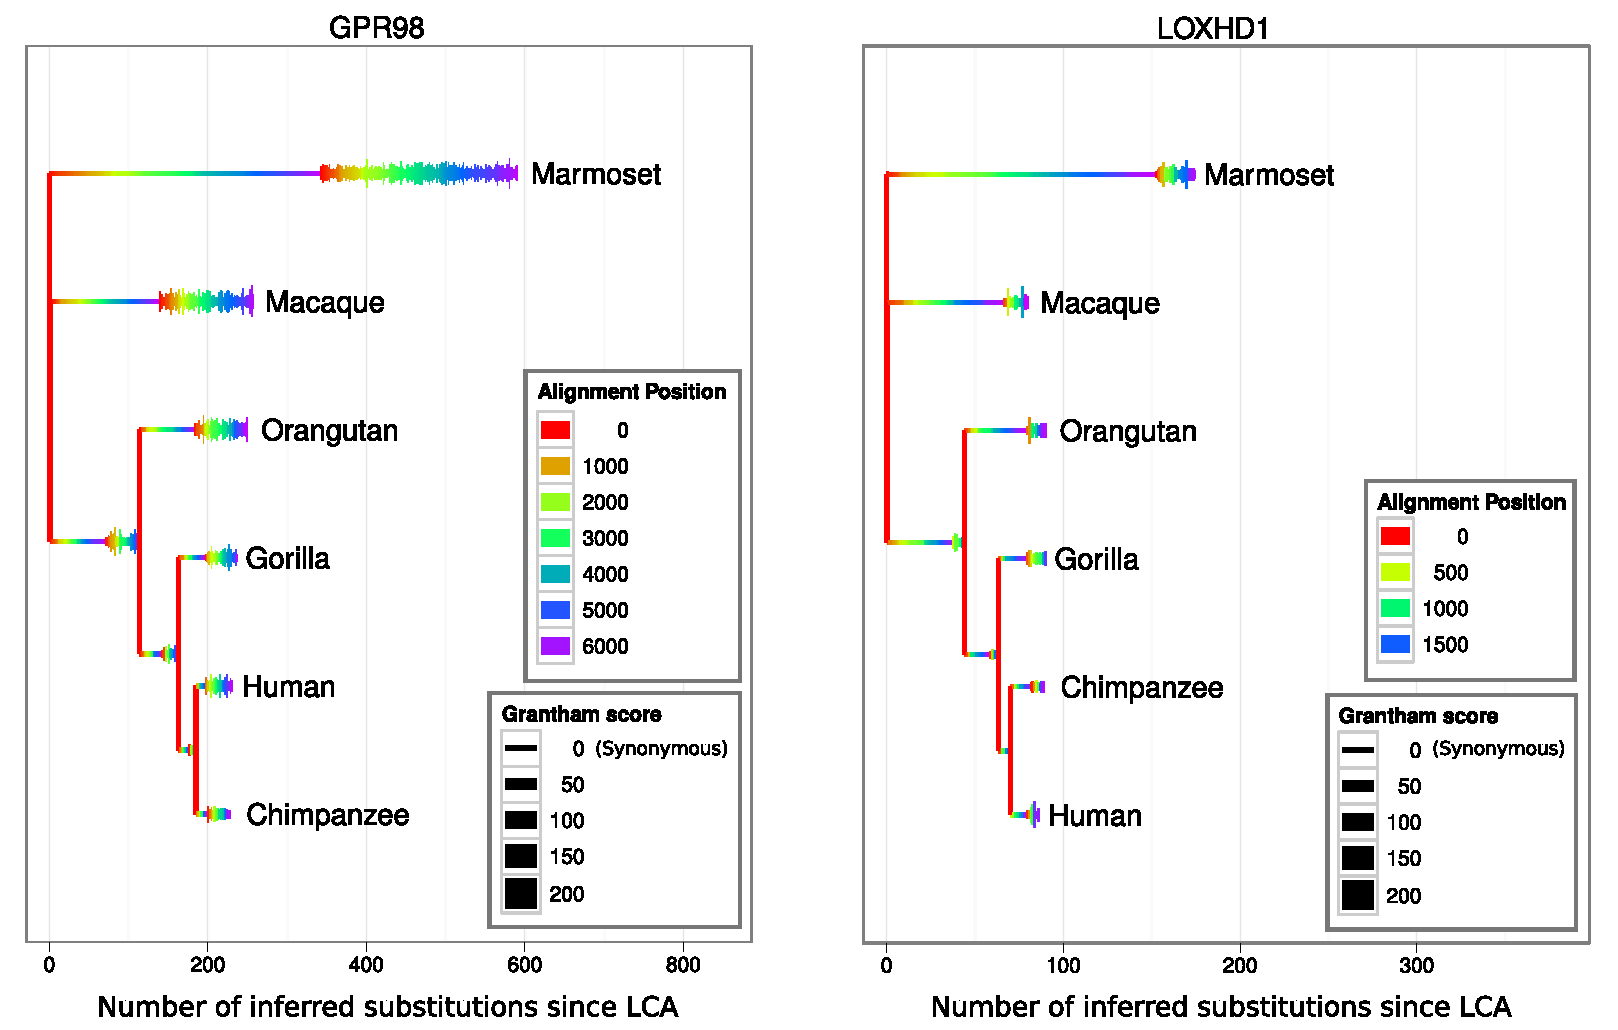
\includegraphics[scale=0.6]{Figs/gorilla_gpr98.pdf}
\caption{Inferred substitution events in the 6-way primate alignments
  of \gene{GPR98} and \gene{LOXHD1}, two hearing-related genes with
  evidence for independent elevated \dnds in \ac{aga}
  species. \ac{paml} was used to infer \ac{ml} ancestral sequences
  \citep{Yang1995} from the 6-way alignment of each gene and
  substitution events were assigned to branches in the phylogeny. Only
  substitutions between nodes where the ancestral reconstruction had a
  posterior probability of $>0.9$ are shown. Substitutions along the
  branch connecting marmoset to the remaining primates were
  arbitrarily assigned to the marmoset terminal branch in the rooted
  view of the phylogeny shown here. Substitutions are drawn as
  rectangles, arranged in a horizontal line for each branch in the
  tree. Within each branch, all \syn substitutions are drawn to the
  left of all \nsyn substitutions; substitutions are then sorted by
  their position in the alignment. Each substitution is colored
  according to its alignment position and scaled according to the
  Grantham score \citep{Grantham1974} between the ancestral and
  derived amino acid.}
\label{fig_gorilla_gpr98}
\end{figure}

Figure \ref{fig_gorilla_gpr98} shows the patterns of \nsyn and \syn
substitutions throughout the 6-way primate phylogeny for two
hearing-related genes, \gene{GPR98} and \gene{LOXHD1}, with strong
signals of parallel elevated \dnds. The much longer \gene{GPR98} has
accrued more substitutions in each branch of the primate tree than
\gene{LOXHD1}, but both genes showed large numbers of \nsyn
substitutions in each of the \ac{aga} species relative to their short
overall branch lengths.

\subsection{Top parallel accelerated genes}

The third method of analysis was a survey of the top parallel
accelerated genes for each species pair and for all three species
using the same \lrtmin statistic described above. Table
\ref{table_gorilla_top_genes} (located in Appendix \ref{ch_lrts} at
the end of this thesis) shows the top 10 accelerated and
positively-selected genes for a variety of \ac{aga} lineages and
tests; the top parallel accelerations according to the \lrtmin
statistic can be found towards the bottom of Table
\ref{table_gorilla_top_genes}.

Among the top genes accelerated across all three lineages are
\gene{LOXHD1}, a gene comprised of PLAT domains which was recently
shown to be necessary for auditory hair cell function
\citep{Edvardson2011}; \gene{ITIH3}, a plasma serine protease
inhibitor potentially involved in prevention of tumor metastasis and
associated with risk of myocardial infarction \citep{Ebana2007}; and
\gene{PARP3}, a member of the ADP ribosyl transferase family which has
recently been characterized as playing a role in telomeric stability,
response to DNA damage, and neural crest development
\citep{Rouleau2011,Boehler2011}. The molecular and medical evidence
for the functional activity of these genes suggests that the elevated
\dnds levels across all three African great apes are not well
explained by a substantial loss of functional constraint; other
possible causes might be relaxed evolutionary constraint due to a
decreased \ac{ne} relative to the primate
background, positive selection due to functional adaptation, or some
combination of the two. 

\section{\acf{go} term enrichments}
\label{sec_gorilla_go}

Gene ontology (GO) term annotations for the ``biological process''
ontology tree were downloaded from release 60 of the Ensembl human
database \citep{Flicek2011} and assigned to the alignment
corresponding to each human gene. Three complementary methods were
used to assign \pvs for \ac{go} term enrichment among the most
accelerated genes for each branch-LRT performed and genes with
evidence of parallel acceleration in a pair of species. For
lineage-specific accelerations, the 95\% \chisq cutoff value of the
branch-LRT was used to identify accelerated genes. Parallel
accelerations for each species pair were identified by genes with a
minimum branch-LRT value of 1.5 in both species of interest (more
detail on the analysis of parallel accelerations is included in
Section \ref{sec_parallel_accel}).

The first test was a standard one-tailed \ac{fet} applied to the 2x2
contingency table of significant / non-significant genes which were
annotated / not-annotated with a given \ac{go} term. The second
method, implemented in the \topgo program \citep{Alexa2006a}, is also
based on the \ac{fet} statistic but additionally compensates for the
structure of the GO hierarchy by iterating through the directed
acyclic graph and removing nodes from consideration when certain
descendant nodes have already shown significant enrichment (see
\citet{Alexa2006a} for complete details of the algorithm). The main
effect of the \topgo algorithm is to identify and remove semantically
repetitive terms (e.g., terms that are nearby in the \ac{go} ontology
and are annotated with similar sets of genes) from the set of most
significantly enriched results by reducing the \pvs of terms with more
highly-enriched neighboring terms. The third method, implemented in
the \texttt{goseq} program \citep{Young2010a}, accounts for a
potential gene length bias in the propensity for a gene to yield a
significant LRT results. As the sequence length can have a strong
impact on the significance of \ac{lrt} results \citep{Anisimova2001}
and some \ac{go} terms tend to contain longer genes
\citep{Young2010a}, I found it important to correct for this when
identifying enriched terms. The \goseq program first uses the set of
gene-wise \pvs and gene lengths to fit a smoothed \ac{pwf} which
predicts the expected proportion of significant accelerations given a
gene’s length. This \ac{pwf} is then used to adjust the identification
of significantly-enriched \ac{go} terms to correct for potential
over-representation of terms with significantly longer or shorter mean
gene lengths. Although the \goseq program was designed primarily for
the functional analysis of RNA-seq data (where gene length bias is a
widely-acknowledged confounding factor) I found it to be effective in
identifying potentially misleading \ac{go} enrichment results for the
current analysis.

The results of the GO enrichment analysis are summarized in Table
\ref{table_gorilla_go}. For each branch model (or pair of species for
parallel accelerations), all terms with a \ac{fet} over-representation
$p<0.05$ and 5 or more significant genes are shown sorted by their
\topgo p-value. Any \topgo or \goseq \pvs above $p=0.05$ are colored
gray instead of black. Terms with non-significant \topgo \pvs are
likely to have a closely-related term with stronger enrichment higher
in the list, while terms with non-significant \goseq \pvs should be
treated with caution due to a detected length bias in the detection of
accelerated genes.

None of the \ac{go} term enrichments for any of the branch-LRTs shown
in Table \ref{table_gorilla_go} remained significant at \ac{fdr}$<0.1$
after applying the \citet{Benjamini1995} correction (results not
shown). The lack of significance after correcting for multiple tests
could be taken as evidence that no strong associations between
accelerated genes and \ac{go} terms existed in these results. However,
it may also be due to a variety of other factors, including limited
power of branch models to detect \dnds shifts, noise in the \ac{go}
annotation of genes, or the specific choice of LRT cutoffs used to
identify significant accelerations. Other studies have avoided the use
of cutoff thresholds by using different tests such as the Mann-Whitney
U test to identify terms with a significantly lower distribution of
\pvs than expected \citep{Clark2003,Kosiol2008}, but this was not done
here. Despite the lack of strongly-controlled statistical
significance, the use of a nominal $p<0.05$ cutoff to identify
enriched GO terms for display in Table \ref{table_gorilla_go} yielded
a limited set of enriched terms for each branch-LRT that summarized
the strongest functional associations with moderately to strongly
accelerated genes.

\section{Comparison with previous genome-wide scans for accelerated or positively-selected genes}

A number of studies have previously investigated the prevalence and
functional associations of \acp{psg} and genes with elevated \dnds in
primate genomes, often using branch-LRTs or branch-site LRTs similar
to those used here. Although these studies have varied widely in the
exact datasets and analytical methods employed, a qualitative and
quantitative comparison their main results helped to appreciate the
variability of previously published genome-wide results in
primates. Table \ref{table_gorilla_studies} presents a summary of
results from the current analysis plus 8 previous genome-wide scans
for accelerated or positively-selected genes. This table was
originally compiled by Stephen Montgomery for the gorilla consortium,
but it has been heavily modified and condensed into the current form.

The proportion of accelerated genes detected using branch-LRT methods
(or close equivalents) ranged from 7.07\% to 20.24\%; results from the
current study, which ranged from 4.64\% in chimpanzee to 5.75\% in
human, was only slightly lower than the typical range of
previously-published values. For the proportion of genes experiencing
positive selection under the branch-site \ac{lrt} (or similar), the
current results results (ranging from 1.23\% in human to 1.66\% in
gorilla) again fell within the lower end of the the published range of
0.43\% to 8.72\%. Most published studies did not show a large
difference in the proportion of accelerated or positively-selected
genes between chimpanzees and humans; our results further confirm this
trend and extend to gorilla the observed consistency in numbers of
lineage-specific accelerated and positively-selected genes between
different \ac{aga} species.

Table \ref{table_gorilla_studies} highlights the wide range of
biological functions and processes that have commonly been found
enriched for genes subject to accelerated evolution or positive
selection. Terms involving immune functions, olfaction, and amino acid
metabolism have most commonly been identified. The GO term enrichments
based on the current branch-LRT results did not recover many terms in
common previous studies. This may be the result of a different type of
sensitivity in the specific branch-\acp{lrt} used here, where gene
accelerations in \ac{aga} lineages \emph{relative to the primate
  background rate} were detected, as opposed to high rates of
evolution on their own. For example, immune genes with high \dnds
ratios across all primates were not likely to be identified as
accelerated in this study, since immune genes tend to be subject to
positive selection throughout the mammalian phylogeny as opposed to
one particular lineage or another (see Chapter
\ref{ch_mammals2}). This could explain the lack of any apparent immune
enrichment in the current results.

Interestingly, the \ac{go} term ``sensory perception of sound'' was
among the top enriched terms in both the gorilla lineage and
gorilla-human parallel accelerated genes. Although previous studies
have detected enrichment for olfaction and visual perception
\citep{Clark2003,Nielsen2005,Macaque2007}, this appears to be the
first genome-wide analysis to provide strong evidence for an abundance
of genes involving sound perception to have been subject to elevated
\dnds ratios in the \ac{aga}. Some evidence was also found for
enrichment of brain-related terms in human and gorilla, including
``brain development'' (Gorilla $p=0.038$, Table
\ref{table_gorilla_go}) and ``nervous system development'' (Human
$p=0.032$, Table \ref{table_gorilla_go}), although both terms may be
subject to a gene length bias and fail to reach $p<0.05$ using the
\goseq method for detecting enriched terms.

\begin{landscape}
\centering \scriptsize
\rowcolors{1}{white}{gray!10}
\begin{longtable}{lllllllb{6cm}}
%\begin{longtable}{>{\raggedright}b{1.8cm}>{\raggedright}b{1cm}>{\raggedright}b{1cm}>{\raggedright}b{1.2cm}>{\raggedright}b{1cm}>{\raggedright}b{.9cm}>{\raggedright}b{.9cm}>{\raggedright}b{8cm}lll}

\toprule
Study & FG Species & Gene Count & Test & Ontology & Accel. & \acp{psg} & Top 5 enriched terms \\
\midrule
\endhead

\midrule
\\
\multicolumn{8}{l}{\normalsize{Table \ref{table_gorilla_studies}} (\emph{continued on next page})} \\
\endfoot

\\[-1.8ex] \hline \hline
\endlastfoot

\input{Tables/gorilla_studies.txt}

\bottomrule

\caption{A comparison of genome-wide studies of primate gene
  evolution. Nine studies of positive selection or accelerated \dnds
  in primates, including the current study, are summarized by various
  factors including the number of genes analyzed, the tests of
  selection performed, the accelerated or positively-selected gene
  count, and the most strongly enriched functional terms. The current
  results were largely consistent with previous results in the
  percentage of accelerated and positively-selected genes
  identified. In contrast, the functional terms detected as enriched
  for accelerated genes varied widely, both within the set of
  previously-published studies and with the current results.}
\label{table_gorilla_studies}

\end{longtable}
\end{landscape}


%\section{Levels of \acf{ils} within and near genes}

%The close proximity of the \ac{hc} and \ac{hc}-G speciation events
%makes \ac{ils} a prominent feature of the genomic relationship between
%human, chimpanzee and gorilla. Regions showing \ac{ils} should not be
%subject to any particular functional constraint, but the \ac{ne} in
%the great ape ancestor is expected to affect the prevalence of ILS,
%causing less ILS in regions of lower ancestral \ac{ne}
%\citep{Hobolth2011}. Strong purifying selection on genes tends to
%reduce the \ac{ne} within and nearby exonic regions due to background
%selection \citep{Charlesworth1993}, so I sought to characterize the
%effect of the strength of purifying selection, as measured by the
%\dnds ratio in the 6-way primate alignments, on the prevalence of
%\ac{ils} within and around protein-coding regions.

%I first looked at patterns of \ac{ils} density within protein-coding
%genes. I separated the 11,534 one-to-one genes into five equally-sized
%\dnds bins, using the \dnds ratios estimated by \ac{paml} using the
%one-ratio M0 model and the filtered 6-way coding alignments. Before
%performing the \ac{ils} masking step described in Section
%\ref{sec_ils_mask}, each alignment site of each gene was assigned a
%substitution pattern according to a comparison of the human,
%chimpanzee and gorilla nucleotides and the orangutan nucleotide. A `1'
%indicated similarity and a `0' indicated dissimilarity to the
%orangutan nucleotide, and for each site a binary ``site pattern'' was
%given by concatenating the values in the order of human, chimpanzee
%and gorilla. Thus, a site where human and gorilla matched the
%orangutan sequence but chimpanzee was different was denoted \texttt{010}. I
%counted and stored the total number of sites with each pattern for
%each gene, skipping all sites with a gap or ambiguous nucleotide in
%any species.

%The most important patterns allowing for discrimination of \ac{ils}
%versus non-\ac{ils} sites are \texttt{110} (a likely substitution in the
%\ac{hc} ancestor), \texttt{101} (a likely substitution in a HG \ac{ils}
%ancestor), and \texttt{011} (a likely substitution in a GC \ac{ils}
%ancestor). Due to the scarcity of substitutions along the short
%ancestral branch, I identified genes with strong evidence of \ac{ils}
%by requiring the presence of more \ac{ils} patterns than non-\ac{ils}
%patterns within a gene---specifically, when $n_{101} + n_{011}$ was
%greater than $n_{110}$. A total of 1,974 genes (17.1\%) showed
%evidence of \ac{ils} at this threshold, which corresponded well with
%the results of the CoalHMM \citep{Hobolth2007} analysis (performed by
%other members of the analysis consortium) where \ac{ils} was inferred
%at 20\% of gene-coding sites.

%\begin{figure}
%\centering
%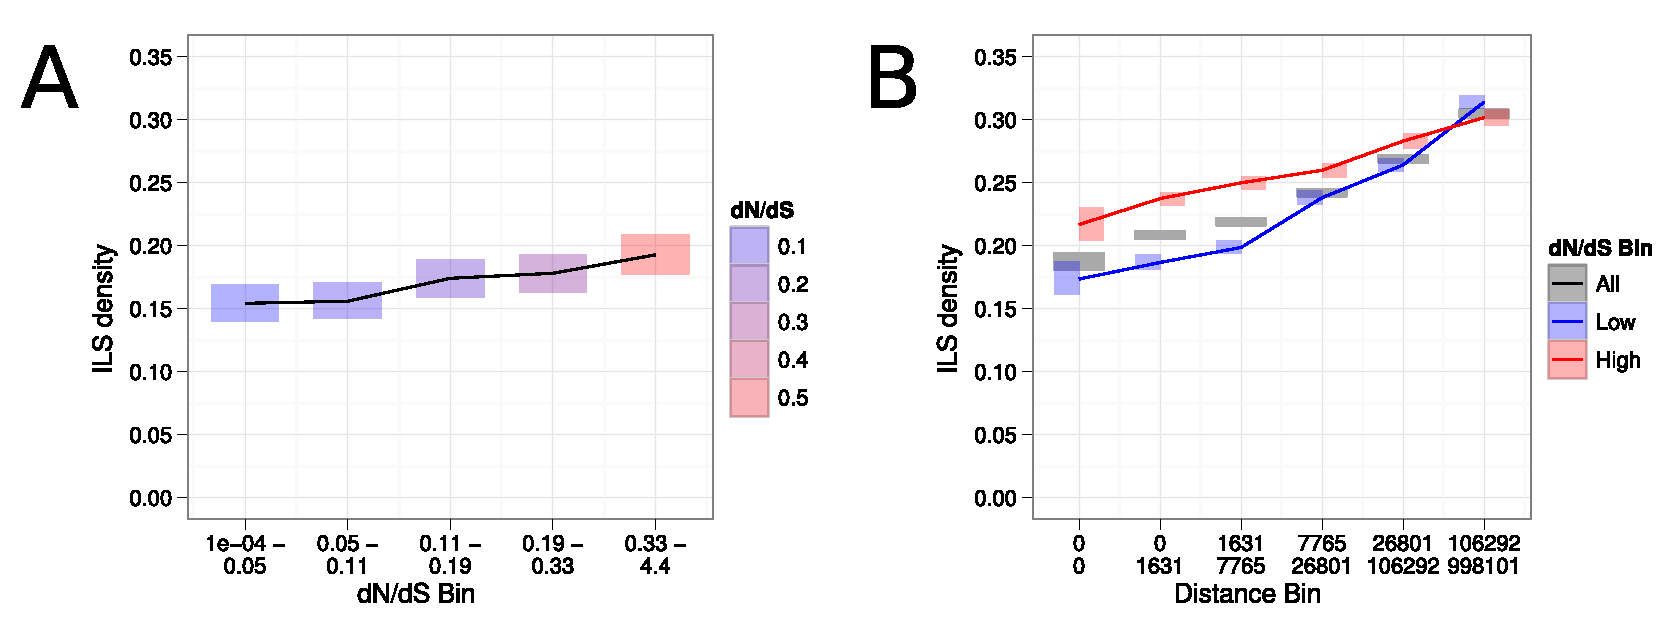
\includegraphics[scale=0.55]{Figs/gorilla_ils.pdf}
%\caption{ILS patterns within and surrounding genes. (A) Genes were
%  separated into five equally-sized \dnds bins and the fraction of
%  genes with strong evidence of \ac{ils} was calculated for each
%  bin. The black line is drawn at the fraction of \ac{ils} genes, and
%  the high and low points of each block corresponds to the 95\%
%  confidence interval. Genes with lower \dnds values contained
%  significantly lower amounts of \ac{ils}, showing the influence of
%  long-term purifying selection on the ancestral \ac{ne}. (B)
%  Overlapping 10kb windows of primate genomic alignments were analyzed
%  for sites showing patterns of \ac{ils}, and the fraction of 10kb
%  windows with strong evidence for \ac{ils} was calculated. Blocks
%  correspond to 95\% confidence intervals. Black, alignments near all
 % genes; red, alignments near genes with high \dnds values; blue,
%  alignments near genes with low \dnds values. Windows near
%  protein-coding exons showed significantly lower amounts of \ac{ils},
%  with the strongest effect being in regions near genes under strong
%  purifying selection.}
%\label{fig_gorilla_ils}
%\end{figure}

%To estimate the correlation between \ac{ils} prevalence and purifying
%constraint in genes, I used the \ac{ils} site patterns and the
%identification threshold described above to calculate the fraction of
%genes with evidence for \ac{ils} within each \dnds bin. A 95\%
%confidence interval was calculated for each \dnds bin based on 1000
%non-parametric bootstrap replicates across genes. Figure
%\ref{fig_gorilla_ils}A shows the result of this analysis, revealing a
%slight but distinct correlation between \ac{ils} density and the
%strength of purifying constraint, with the \ac{ils} density ranging
%from 16\% in genes with the lowest primate \dnds to 19\% in genes with
%the highest \dnds. This was consistent with the expectation that
%\ac{ils} is depleted from regions subject to purifying selection due
%to persistent background selection and a locally decreased \ac{ne}.

%I used a similar approach to investigate the effect of \dnds levels on
%\ac{ils} density in regions surrounding protein-coding genes. First,
%counts of \ac{ils} and non-\ac{ils} patterns were collected for
%segments of Ensembl’s 6-way primate \ac{epo} alignments corresponding
%to 10kb windows of the human genome spaced at 3.3kb intervals,
%yielding 470,344 individual alignment regions. The proximity of each
%region to a protein-coding gene was calculated as the distance from
%the region's center point to the nearest human protein-coding exon. (
%(A distance of zero was assigned if the region's center point was
%within an exon). The identity and \dnds value of the gene containing
%the nearest exon was also stored. Each 10kb region was then identified
%as \ac{ils} or non-\ac{ils} based on which type of site pattern was
%more frequent within that region, as above. Regions were then
%separated into equally-sized bins based on their distance to the
%nearest exon (with a separate bin for windows with a distance of
%zero), and the density of \ac{ils} regions within each bin was
%calculated. Figure \ref{fig_gorilla_ils}B shows the resulting
%proportion of \ac{ils} regions, binned by distance to the nearest
%gene.

%A total of 24.8\% of windows across all distance bins were classified
%as having evidence of \ac{ils}. The same calculations were then
%repeated for windows whose nearest gene was in the lowest 25\%
%quantile (\dnds$<0.05$; Figure \ref{fig_gorilla_ils}B, blue bars and
%line) and in the highest 25\% quantile (\dnds$>0.24$; Figure
%\ref{fig_gorilla_ils}B, red bars and line). The effect of background
%selection on gene-flanking regions of the genome could be clearly seen
%in the reduced \ac{ils} density in windows near to exons; furthermore,
%this effect scaled with the strength of purifying selection on a given
%gene and could be observed in windows further than 100kb from the
%nearest exon.

\section[Genome-wide \dnds ratios in the African great ape phylogeny]{Genome-wide \dnds ratios in the \acf{aga} phylogeny}

The gorilla genome also provided an opportunity to examine global
trends in the evolutionary dynamics of the \acp{aga} and
their ancestral populations. I used the genome-wide set of coding
alignments to examine lineage-specific \dnds estimates across the
six-primate phylogenetic tree.

Two broad categories of methods have commonly been employed to
estimate ancestral \ac{ne} from comparative genomics data: methods
based on estimating the variance of species divergence times or tree
topologies in samples of coding or noncoding DNA, and methods based on
estimating lineage-specific \dnds ratios in protein-coding genes.

Over the past two decades a number of groups have applied methods
based on the first approach (using variance in divergence times / tree
topologies) to the estimation of primate ancestral populations
(\citet{Takahata1997,Chen2001,Holbolth2007,Burgess2008}; reviewed in
\citet{Siepel2009a}). Despite significant differences in the inference
methods and sizes of datasets used, most analyses were in agreement
that the \ac{ne} of ancestral hominoids was considerably larger than
that found in most present-day populations. However, no consensus
appears to have emerged regarding the absolute \acp{ne} of primate
ancestral populations, and the precision of estimates has been lacking
\citep{Siepel2009a}.

The second general approach is based on comparing lineage-specific
\dnds values estimated from a large amount of aligned protein-coding
sequence. Theory predicts that larger populations should exhibit, on
average, lower \dnds values due to increased efficacy of purifying
selection \citep{Ellegren2008}, and results from several genome-wide
analyses consistently confirmed this trend
\citep{LindbladToh2005Genome,Macaque2007,Sequencing2005a,Warren2008b,Kosiol2008}. All
of these studies were based on alignments of orthologous genes in at
least human and mouse (in addition to other species), and in every
case human had a higher mean \dnds value than mouse. This was
consistent with the theory, given the expectation based on ecological
studies of a much large \ac{ne} in mouse compared to human
\citep{Ellegren2008}. Furthermore, \citet{Ellegren2008} identified a
strong negative correlation between the lineage-specific \dnds
estimates from \citet{Kosiol2008} and the log-\ac{ne} as estimated
from polymorphism data. Within primates, all of the above studies
which included macaque showed it to have a lower \dnds than human and
chimpanzee. There does exist some disagreement regarding the relative
\dnds of human and chimpanzee, however: \citet{Macaque2007} found a
mean \dnds of 0.175 for chimpanzee and 0.169 for humans, while
\citet{Kosiol2008} found a mean \dnds of 0.245 for chimpanzee and
0.249 for humans. While the two values are very similar in both cases,
this discrepancy indicates some remaining uncertainty regarding the
\ac{ne} of humans and chimpanzees since their divergence event 4-6
\ac{myr} ago. Furthermore, the association between sequencing and
assembly errors and inflated estimates of positive selection
\citep{Schneider2009} suggests that lower-quality genomes may be prone
to increased \dnds estimates as a result of such errors, especially in
closely-related primate genomes.

I used \ac{paml} to estimate genome-wide \dnds levels for each branch
in the six-species primate phylogeny from the 11,534 aligned 1-to-1
orthologous genes assembled here. Two alignments were created: an
unfiltered alignment, created by concatenating the alignment of each
gene after sequences were filtered for sequence quality but before the
window-based filter for clustered \nsyn substitutions and the filter
for \ac{ils}-patterned substitutions were applied; and a filtered
alignment, created by concatenating the final alignment of each gene
that was used for the branch-LRT analysis. Both alignments were 7.263
million codons in length. Before being input to \ac{paml}, all columns
containing a gap character or `N' in any species were removed. As
expected, more columns were removed from the filtered alignment due to
additional `N's from the window-based masking procedure: the final
unfiltered alignment contained 5.91 million codons and the final
filtered alignment contained 5.89 million codons. A single \dnds ratio
was first estimated for each alignment using the M0 codon model,
yielding 0.220 for the unfiltered and 0.218 for the filtered
alignment. Separate \dnds values for each branch were then estimated
from each alignment using the free-ratios model implemented in
\ac{paml} (parameter \texttt{model=1}). Because \ac{paml} estimates
parameters based on an unrooted tree using reversible models of
evolution, any estimates of \dnds on the outermost branch (i.e., the
branch connecting the H/C/G/O/M ancestor to marmoset) were ambiguous
as to whether they occurred on the branch leading to marmoset or the
branch leading to the other primates; thus, marmoset was considered an
outgroup in this analysis.

\begin{figure}
\centering
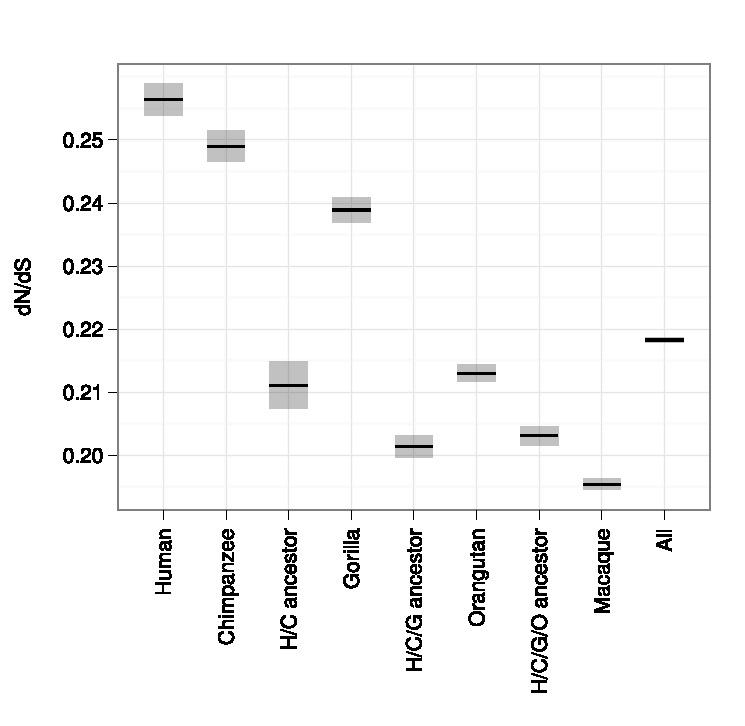
\includegraphics[scale=0.8]{Figs/gorilla_dnds.pdf}
\caption{Genome-wide \dnds values in 5 primate species and their
  ancestral lineages. \dnds ratios were estimated from concatenated
  alignments of 1-to-1 orthologs from six primate species using the
  free-ratios model in \ac{paml}. The most distant aligned species,
  marmoset, was used as an outgroup. Each estimated \dnds ratio is
  plotted as a horizontal line surrounded by a gray box corresponding
  to the standard error estimated by \ac{paml}. Ancestral lineages are
  labeled with the first characters of their descendant species.}
\label{fig_gorilla_dnds}
\end{figure}

\begin{table}
\centering \scriptsize
\begin{tabular}{lrrrrrr}
\toprule
 & \multicolumn{3}{c}{Filtered} & \multicolumn{2}{c}{Unfiltered} & \% \dnds change \\
\cmidrule(r){2-4} \cmidrule(r){5-6}
Branch & \ds & \dnds & S.E. & \dnds & S.E. & (unfiltered vs. filtered) \\
  \midrule

\input{Tables/gorilla_dnds.txt}
\bottomrule
\end{tabular}
\caption{Genome-wide \ds and \dnds values in 5 primate species and
  their ancestral lineages. \dnds ratios were estimated from
  concatenated alignments of 1-to-1 orthologs from six primate species
  using the free-ratios model in \ac{paml}. The unfiltered alignments
  were collected before clustered \nsyn substitutions and sites with
  \ac{ils} patterns were removed. The most distant aligned species,
  marmoset, was used as an outgroup. Ancestral lineages are labeled
  with the first characters of their descendant species. The M0 model
  was used to estimate values for the row labeled
  ``All''. S.E.---standard error of the \dnds ratio estimate
  calculated by \ac{paml}.}
\label{table_gorilla_dnds}
\end{table}

The resulting genome-wide estimates of \ds and \dnds for each branch
are given in Table \ref{table_gorilla_dnds} and plotted in Figure
\ref{fig_gorilla_dnds}. I found that human had a slightly but
significantly higher overall \dnds than both chimpanzee and gorilla
(\dnds$=$0.256, 0.249, 0.239, respectively) and that orangutan,
macaque, and the ancestral lineages all had lower overall \dnds values
than the terminal \ac{aga} branches, ranging from 0.195 for macaque to
0.211 for the human-chimpanzee ancestor. These results were in strong
agreement with equivalent estimates from \citet{Kosiol2008}, who found
overall \dnds values of 0.249, 0.245, and 0.191 for human, chimpanzee,
and macaque, respectively.

A comparison of the global \dnds values from the unfiltered versus the
filtered alignments in Table \ref{table_gorilla_dnds} revealed that
the unfiltered alignments generally yielded higher \dnds values, but
the magnitude of change varied dramatically between branches. The
human terminal branch and all of the ancestral branches showed less
than a 1\% decrease in \dnds as a result of the alignment filtering,
while chimpanzee, gorilla, orangutan, and macaque all showed greater
than 1\% decrease in \dnds. Since the window-based masking procedure
was only applied to clusters of substitutions inf the terminal
branches, the lack of change in \dnds ratios along the ancestral
branches was expected. The smaller magnitude of change in human
(0.39\%) compared to the other extant primate genomes (ranging from
1.03\% to 4.18\%) indicated that the filtering procedure resulted in
far more \nsyn substitutions being removed from non-human sequences
than from human. Interestingly, the magnitude of the \dnds change for
non-human terminal branches appeared to correlate negatively with the
\ds of that branch. Gorilla and chimpanzee, with \ds$=0.0077$ and
\ds$=0.0055$ respectively, both had a $\sim$4\% shift; orangutan, with
\ds=$0.016$, had a $\sim$2\% shift; and macaque, with \ds$=0.032$, had
a $\sim$1\% shift. These observations were consistent with the trend
expected if each genome contained a similar number of erroneous or
misaligned bases, as the larger number of true \nsyn and \syn
substitutions species with longer terminal branch lengths would tend
to ``dilute out'' the signal of elevated \dnds resulting from
misaligned bases. In sum, the comparison between filtered and
unfiltered \dnds levels provided further validation of the use of the
window-based substitution filter. The application of the filter hardly
affected the estimated \dnds ratio of the finished-quality human
genome, but it resulted in branch-length dependent decreases in \dnds
in the lower-quality nonhuman primate genome assemblies. Notably,
chimpanzee showed a marginally higher \dnds than human in the
unfiltered alignment and a significantly lower \dnds than human in the
filtered alignment.

An additional consideration in the interpretation of global \dnds
values was that genes are evolutionarily heterogeneous entities, with
each gene composed of sites evolving under different amounts of
purifying and positive selection due to varying functional and
biological constraints \citep{Whelan2008}. The genome-wide \dnds
estimates in Table \ref{table_gorilla_dnds} were obtained using the
free-ratios codon model, with one \dnds ratio per branch but a
constant \dnds across all alignment sites. Each \dnds ratio estimated
under this model could thus be considered an ``average'' value,
resulting from the combination of sites under strongly purifying,
slightly purifying, neutral and positive selection into a single
alignment. 

This averaging across genes and sites causes two problems for
comparative studies: first, the comparison of genome-wide \dnds values
from different studies is difficult, as the specific genes chosen for
analysis can have a significant impact on the overall results
\citep{Ellegren2008}. Second, the inclusion of sites with very
different selective pressures might decrease the resolution with which
lineage-specific differences in \dnds (and thus \ac{ne}) could be
detected. This is because some fraction of protein-coding sites may
evolve neutrally or under positive selection. Neutrally-evolving sites
in genes should show no relationship with \ac{ne}, and positive
selection should show the opposite effect, with higher \dnds values
with large \ac{ne} due to increased efficacy of positive
selection. Although the proportion of such sites is likely small, they
may obscure the connection between \dnds and \ac{ne}.

One way to better understand the effect of heterogeneously evolving
sites on genome-wide \dnds analyses was to separate out sites with
different selective pressures and analyze each group independently. I
took this approach by separating protein-coding sites into bins based
on their estimated sitewise selective pressure across mammals and
separately analyzing the set of sites within each bin. Sitewise
selection pressures were estimated for all 11,534 genes by applying
\ac{slr} \citep{Massingham2005} to coding alignments of all Eutherian
orthologs downloaded from the Ensembl Compara database. (Note that for
this analysis, the protein-based MCoffee alignments calculated by the
\ens pipeline were used directly.) The \sw \ac{lrt} statistic
calculated by SLR was used to sort all sites by their strength of
evidence for non-neutral selection. Sites were then split into five
bins corresponding to the following cumulative percentiles of the LRT
statistic: 0--0.05, 0.05--0.33, 0.33--0.67, 0.67--0.98, and
0.98--1.0. These ranges were chosen so that three bins of roughly
equal size covered the bulk of sites, while two bins focused on the
5\% most strongly purifying sites and the 2\% of sites with strongest
evidence for positive selection. All sites from each bin were
concatenated into one alignment and analyzed with the \ac{paml}
free-ratios model as described above.

\begin{figure}
\centering
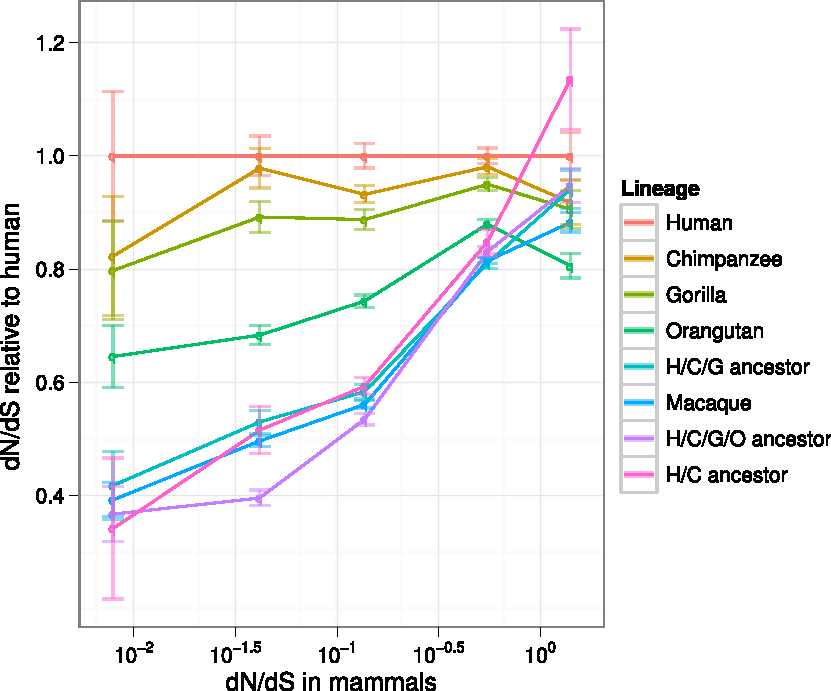
\includegraphics[scale=0.9]{Figs/gorilla_dnds2.pdf}
\caption{Genome-wide branch-specific \dnds ratios in 6-way primate
  alignments binned by \sw selection pressure. Alignment sites were
  sorted by the \sw selection pressure estimated by \ac{slr} in
  mammals, assigned to one of five bins (more details in text),
  concatenated within each bin, and analyzed with \ac{paml} using the
  free-ratios codon model. Estimated \dnds ratios are plotted with the
  human \dnds for each bin on the x-axis and the \dnds for each branch
  (expressed as a fraction relative to the human \dnds in that bin) on
  the y-axis. Lines are drawn connecting estimates from the same
  branch in different bins, and standard errors reported by \ac{paml}
  are shown with error bars. Note the log scale on the x-axis.}
\label{fig_gorilla_dnds2}
\end{figure}

The lineage-specific \dnds ratios estimated from alignments binned by
\sw mammalian selective pressure are shown in Figure
\ref{fig_gorilla_dnds2}. Results from each bin are spread across the
x-axis, and the \dnds ratio for each branch is plotted on the y-axis
as a fraction relative to the human \dnds in that bin.

The 4 lowest \dnds bins showed the same general trends in \dnds levels
as the combined analysis: with human, chimpanzee, and gorilla yielded
the highest \dnds values, followed by orangutan, and finally a cluster
of macaque and the ancestral lineages contained the lowest \dnds
ratios. The H/C/G/O ancestral lineage appeared to have evolved with a
slightly lower \dnds than the other ancestral lineages, though this
difference was only apparent in the 2nd and 3rd bins.

Moving from bins with lower human \dnds to bins with higher human
\dnds, there was a distinct trend across all lineages towards
increased \dnds values relative to human. In the second-lowest bin,
where human had a \dnds ratio of $\sim$0.05, the \dnds difference
between lineages was much stronger than in the second-highest bin,
where human had a \dnds ratio of $\sim$0.55. This trend was consistent
with the expected decrease in the differential effects of \ac{ne} in
sites subject to weaker purifying (e.g., more nearly neutral)
selection.

The pattern of genome-wide \dnds levels in the highest bin---representing the top
2\% of alignment sites ordered by the LRT statistic, and thus the 2\%
of sites with the greatest site-specific evidence for positive
selection across Eutherian mammals---was distinct from the other 4
bins and warrants further mention. The human \dnds in this bin was
$\sim$1.4, confirming that this subset of alignment sites did indeed
contain a number of sites subject to positive selection. Most of the
terminal and ancestral branches showed a continuation within this bin
of the general trend of increasingly similar \dnds estimates between
lineages, with values for most branches clustered to around
$\sim$88\%--95\% of the human \dnds. However, the \ac{hc} ancestral
lineage showed strikingly increased \dnds values in the highest bin,
and the orangutan branch showed strikingly decreased values. Whereas
the \ac{hc} branch was at $\sim$85\% of the human value in the 4th
bin, its value was $\sim$110\% that of human in the highest bin. In
contrast, orangutan went from $\sim$90\% in the 4th bin to $\sim$80\%
in the highest bin. Such a strong deviation from the consistent trends
observed in the other lineages and other bins suggested that some
effect other than a difference in \ac{ne} may have caused an increase
or decrease in the prevalence of \nsyn substitutions at sites with
evidence for positive selection across Eutherian mammals.
%One approach to
%investigating this artifact more deeply would be to identify the
%subset(s) of genes which contribute most strongly to these lineages’
%deviations from the trend.

\section{Conclusions}

The gorilla genome sequence provided an opportunity to investigate
patterns of recent molecular evolution through comparison to the
genomes of other \acp{aga} and more distantly-related
primates. Relative to human, gorilla was neither the closest
\citep{Sequencing2005a} nor the most distantly-related primate to have
its genome sequenced \citep{Macaque2007,Locke2011}, limiting the
expectation that its sequence might help identify entirely novel
human-specific or primate-specific evolutionary trends. Instead, the
aim of this chapter was to leverage gorilla's intermediate
phylogenetic position to help assess how variable or consistent
patterns of evolutionary constraint have been throughout the evolution
of the \ac{aga} clade.

This was done through a number of distinct but complementary
analyses. First, a series of branch-LRTs were used to identify genes
with evidence of elevated \dnds along different branches of the
primate phylogeny. The three \acp{aga} showed similar overall counts
of accelerated genes, and a number of distinct functional categories
were enriched for accelerated genes; sound perception and hearing
genes showed especially strong evidence for independent acceleration
in \ac{aga} species. These LRT results were also used to quantify
levels of parallel acceleration between pairs of \ac{aga} species,
showing a greater amount of parallel acceleration between gorilla and
human than between gorilla and chimpanzee. Finally, the set of
genome-wide primate alignments was used to estimate lineage-specific
\dnds ratios, providing precise estimates of the \acf{ne} in the
recent and distant evolution of gorilla and the \acp{aga}.

In conclusion, this study used codon models of evolution to place the
gorilla genome within the context of the other \acp{aga} and
primates. The wealth of data afforded by genome-wide datasets allowed
confident conclusions to be made regarding the variability of
molecular evolutionary patterns among the \acp{aga} species, revealing
a largely uniform landscape of recent \ac{aga} gene evolution which
was generally in accordance with previously-published studies. On the
other hand, the extent to which strong statements could be made about
individual genes appeared somewhat limited by the small amount of
divergence within the \ac{aga} clade. Furthermore, the evidence for
lower \acp{ne} in the recent history of \ac{aga} species suggests that
patterns of recent \ac{aga} and human evolution over the past 6-10
\ac{myr} have been dominated by genetic drift and relaxed
constraint. Still, future work on the analysis of genes with the
strongest signals of elevated \dnds---perhaps incorporating
information from the wider history of mammalian evolution into the
identification of such genes---may identify genes that have played
important roles in the ancient and continued evolution of the
\aclp{aga}.

%************************************************
\chapter{Conclusions}
\label{ch_conclusions}
\acresetall
%************************************************

In this thesis, I proposed to explore the application of mathematical
models of evolution to better understand the patterns of natural
selection acting on mammalian protein-coding genes. Throughout the
analyses and discussions presented in the five preceding chapters, two
recurrent dichotomies underscored significant remaining challenges and
opportunities in contemporary comparative genomics: the distinction
between truth and error in identifying orthologs and aligning
protein-coding sequences, and the distinction between neutral
evolution and natural selection in explaining their evolution.

The theme of error was at the forefront of Chapter \ref{ch_indels1},
where simulated protein-coding sequence evolution was used to
investigate the impact of alignment error on the detection of \sw
positive selection. The best aligners showed a good ability to
accurately identify homologous codons, even in very divergent
sequences prone to large amounts of biological insertion and
deletion. On the other hand, \emph{post-hoc} methods for alignment
filtering seemed unable to improve on the best aligners in
distinguishing true from erroneous homology. The parameters used for
simulation were chosen to approximate the evolution of mammalian or
vertebrate genes, and a wide range of divergence levels (from
primate-like divergences to yeast-like divergences) was tested. Likely
owing to differences in the prevalence of positive selection and in
the distribution of selective pressures, some discrepancy was observed
between the results of the current simulation and those of a similar
study focused on the application of alignment filters to the study of
HIV-1 evolution.

Even with powerful aligners available, errors were abundant in the
alignments of mammalian and primate genes. Difficulties in identifying
orthologs (Chapter \ref{ch_orthologs}), sequencing and assembling DNA
(Chapter \ref{ch_mammals1}), gene conversion events (Chapter
\ref{ch_mammals2}) and incomplete lineage sorting (Chapter
\ref{ch_gorilla}) were all identified as plausible, and in some cases
unavoidable, sources of error in the studies presented here. In
Chapters \ref{ch_mammals1} and \ref{ch_gorilla} I described a
heuristic approach to masking sequences or alignment regions with
suspiciously dense clusters of \nsyn substitutions; further
development of this approach, including quantification of its ability
to reduce false positives in downstream analyses, may be a fruitful
area for future research.

The ability to distinguish between neutral evolution and natural
selection is a major advantage of codon-based models of evolution in
comparison to their nucleotide or amino acid counterparts. The
application of codon models to the analysis of a large number of
mammalian genomes showed how they can be used to explore the patterns
of selective constraint experienced by protein-coding genes. It was
clear that the additional mammalian genomes made available by the
\acl{mgp} increased the power to detect purifying and positive
selection, expanding the catalogue of genes with statistically
significant evidence for positive selection and showing that \acp{psg}
often contain interwoven patterns of purifying and positive
selection. In comparing the evolution of different mammalian groups,
however, the distinction between drift and constraint was
\changeme{less certain}. Chapters \ref{ch_mammals1} and
\ref{ch_mammals2} found lower numbers of \acp{psc} and \acp{psg}, and
lower average \dnds ratios within genes, in glires compared to
primates and laurasiatheria. Given the well-established differences in
\ac{ne} between glires and primate species, the nearly neutral theory
provided a good explanation for the different \dnds ratios. The
difference in levels of positive selection was harder to explain with
confidence, but a number of factors may have contributed: widespread
fixation of deleterious mutations in primates and laurasiatheria as a
result of lower long-term \ac{ne}, higher error rates for detecting
\acp{psc} in primates due to the shorter total branch length, or a
historically greater prevalence of positive selection in primates and
laurasiatheria could all plausibly be responsible for the observed
species-dependent differences in patterns of positive selection.

Future work could be directed towards an improved understanding of
these differences. Results from the study of genetic variation in
present-day populations may help shed light on levels of purifying and
positive selection in the recent history of diverse mammals, and
reasonable extrapolations deeper into history may provide new insight
into the patterns observed here. Alternatively, the development of
evolutionary models that explicitly account for changing \ac{ne} may
help us better understand the impact of \ac{ne} on the evolution of
mammalian genomes. The results from Chapter \ref{ch_gorilla}, which
estimated a lower historical \ac{ne} for human than for all other
\ac{aga} lineages examined, provided additional support for the
development of advanced evolutionary models incorporating the effects
of \ac{ne} within the framework of the nearly neutral theory.

The cost of sequencing a human-sized genome has dropped nearly
700-fold during the four years of my Ph.D. research (from \$7M to
\$10k per genome, \citep{Wetterstrand2011}), and ambitious yet
realistic plans have been drawn to sequence several thousand
vertebrate genomes in the near future \citep{Haussler2009}. With
respect to the rapidly-developing technology of genome sequencing, two
concluding points seem especially pertinent. First, the increasing
amount of available genomic data will be matched perhaps only by the
increasing number of potential false discoveries made possible by the
error-prone nature of such high-throughput data collection and
analysis. Whereas researchers used to manually fix alignment or
sequencing errors ``by eye'', this approach clearly does not work at a
genomic scale, and well-designed automated methods should almost
always outperform manual assessment. As a result, a rigorous and
comprehensive understanding of sources of error in comparative
genomics, combined with widespread adoption of best practices for
reducing their impact on all types of downstream evolutionary
analyses, will become increasingly important. Second, given the small
number of observed fixed differences in comparative studies of humans
and closely-related primates, it seems likely that the continued
development of more complex evolutionary models and inference methods,
rather than the sequencing of more primate genomes, has the most
potential to significantly improve our power to identify and
understand the molecular signatures of adaptive changes in our recent
evolutionary past.

\chapter{Appendix A}
\section*{Publications}

During the course of my Ph.D. research I have contributed to the following articles:

\begin{bibunit}[Classes/greg-thesis.bst]
\nocite{Jordan2008alt}
\nocite{Bishop2009alt}
\nocite{Sipos2011alt}
\nocite{Albers2011alt}
\nocite{LindbladToh2011alt}
\nocite{Jordan2011alt}
\def\chapter*#1{}
\renewcommand{\bibsection}{\chapter*{\bibname}}
\putbib[references]
\end{bibunit}

\chapter{Top accelerated and positively-selected genes in the African great apes}
\label{ch_lrts}

\begin{scriptsize}
\begin{longtable}{>{\raggedright}b{1.5cm}lrrrrrrrrrrr}

\toprule

 & & & \multicolumn{2}{c}{M0 \dnds} & \multicolumn{2}{c}{Subst.} & \multicolumn{3}{c}{Branch-LRT} & \multicolumn{3}{c}{Branch-site LRT} \\
\cmidrule(r){4-5} \cmidrule(r){6-7} \cmidrule(r){8-10} \cmidrule(r){11-13}
Test & Gene & Len. & Mam. & Pri. & N & S & LRT & $p$ & \acs{fdr} & LRT & $p$ & \acs{fdr} \\
\midrule
\endhead

\\
\multicolumn{12}{l}{\normalsize{Table \ref{table_gorilla_top_genes}} (\emph{continued on next page})} \\
\endfoot

\\[-1.8ex] \hline \hline
\endlastfoot

\input{Tables/gorilla_top_genes.txt}
\bottomrule

\caption{Genes with the stongest evidence for acceleration and
  positive selection in gorilla and the African great
  apes. Mam.---mammals; Pri---primates; N---the number of \nsyn
  substitutions; S---the number of synonymous substitutions; LRT---the
  likelihood ratio test statistic; FDR---the false discovery rate
  calculated using the \citet{Benjamini1995} method.}
\label{table_gorilla_top_genes}
\end{longtable}
\end{scriptsize}


\backmatter % book mode only

\def\bibpreamble{\emph{After each reference, a list of pages from
    which the reference is cited is included in brackets.}}

\bibliographystyle{Classes/greg-thesis.bst}
\bibliography{references} % References file
\end{document}
